\documentclass[10pt,a4paper,oneside,fleqn,english]{memoir} 
\usepackage{beamerarticle}           % do not remove! 
\usepackage{hyperref}
\usepackage{booktabs}
\usepackage{tikz}
\usetikzlibrary{positioning}
\usepackage{listings}
\usetikzlibrary{positioning,shapes,arrows.meta}
\usetikzlibrary{positioning, matrix, calc, trees}
\tikzset{out/.style={draw, rectangle, rounded corners, fill=blue!10, minimum height=8mm, minimum width=20mm, align=center}}
% \usepackage[backend=biber]{biblatex}
% \bibliography{bib/mainBiblio}
% This file loads the style files below
% Content has been distributed across multiple style files for easier maintenance and better overview

\usepackage{styles/vubhousestyle}  % VUB house style elements
\usepackage{styles/ulbhousestyle}  % ULB house style elements
\usepackage{styles/myListings}     % my code listings settings
\usepackage{styles/myPackages}     % my loaded packages
\usepackage{styles/myPageSetup}    % my page setup for report/thesis and slides
\usepackage{styles/myBibSettings}  % my bibliography settings
\usepackage{styles/myCommands}     % my own commands
\usepackage{styles/myEnvironments} % my own environments
\usepackage{styles/myDrawingStuff} % my own drawing commands 



          % load my style files
% This template provides these three title pages:
%  VUB title page                
%  BRUFACE title page            
%  ULB title page 

% Important: if you want to remove content from the title page, you have to remove the content from within the curly braces of the relevant command.

% For example: if you want to remove the subtitle from the vub title page,
% you have to replace the command:
% \newcommand\vubsubtitle{optional subtitle} by
% \newcommand\vubsubtitle{}

% Each title page has its own file where the content must be specified:
%% Specify the content for the VUB title page and title slide

% Pick your type of work
\newcommand\vubtypeofwork{Master thesis submitted in order to be awarded the degree of}
%\newcommand\vubtypeofwork{Bachelor thesis}
%\newcommand\vubtypeofwork{Masterproef ingediend met het oog op het behalen van de graad van}
%\newcommand\vubtypeofwork{Bachelorproef}
%\newcommand\vubtypeofwork{} % use this to remove it from the title page

% Pick your program
\newcommand\vubprogram{Master of Science in Engineering Technology}
%\newcommand\vubprogram{Bachelor of Science in Engineering Technology}
%\newcommand\vubprogram{Master of Science in de Industriële Wetenschappen}
%\newcommand\vubprogram{Bachelor of Science in de Industriële Wetenschappen}
%\newcommand\vubprogram{} % use this to remove it from the title page


% Pick your profile
\newcommand\vubprofile{Electromechanical Engineering - sustainable energy}
%\newcommand\vubprofile{Electromechanical Engineering - aeronautics}
%\newcommand\vubprofile{Electromechanical Engineering - mechatronics}
%\newcommand\vubprofile{Electromechanical Engineering - sustainable energy}
%\newcommand\vubprofile{Electromechanical Engineering - transport technology}
%\newcommand\vubprofile{Electronics-ICT - embedded systems}
%\newcommand\vubprofile{Electronics-ICT - networks}
%\newcommand\vubprofile{Elektromechanica - duurzame energie}
%\newcommand\vubprofile{Elektromechanica - luchtvaarttechnologie}
%\newcommand\vubprofile{Elektromechanica - mechatronica}
%\newcommand\vubprofile{Elektromechanica - vervoertechnologie}
%\newcommand\vubprofile{Elektronica-ICT - ingebedde systemen}
%\newcommand\vubprofile{Elektronica-ICT - netwerken}
%\newcommand\vubprofile{} % use this to remove it from the title page

% this command concatenates the type + program + profile defined above
\newcommand\vubpretitle{\vubtypeofwork\\ \vubprogram:\\ \vubprofile}
%\newcommand\vubpretitle{} % use this to remove it from the title page

\newcommand\vubtitle{Stochastic, bottom-up modelling of energy demand under climate uncertainty.} 

\newcommand\vubsubtitle{}
%\newcommand\vubsubtitle{} % use this to remove it from the title page

\newcommand\vubstudent{Alexandre Musongela} % first name last name

\newcommand\vubyear{2025-2026}           % academic year
\newcommand\vubpresentationdate{\today}  % presentation date, automatically set to today, replace with fixed day if required

%\newcommand\vubNDA{Under NDA} % English version
%\newcommand\vubNDA{Onder NDA} % Dutch version
\newcommand\vubNDA{} % use this to remove it from the title page

\newcommand\vubpromoters{promoter: prof. Svend Bram} % English version
%\newcommand\vubpromoters{promotor: ...} % Dutch version
%\newcommand\vubpromoters{} % use this to remove it from the title page

\newcommand\vubsupervisors{supervisor: Yassine El Alali}  % English version
%\newcommand\vubsupervisors{begeleider: ...} % Dutch version
%\newcommand\vubsupervisors{} % use this to remove it from the title page

\newcommand\vubfaculty{ENGINEERING SCIENCES}      % English version
%\newcommand\vubfaculty{INGENIEURSWETENSCHAPPEN}  % Dutch version
%\newcommand\vubfaculty{} % use this to remove it from the title page





      % content VUB title page     
%% Specify the content for the BRUFACE title page and title slide

% Important: if you want to remove content from the title page, you have to remove the content from within the curly braces of the relevant command. For example: if you want to remove the subtitle from the title page, you have to replace the command \newcommand\ulbsubtitle{optional subtitle} by \newcommand\ulbsubtitle{}

% Pick your program:
%\newcommand\brufaceprogram{Electromechanical Engineering: Aeronautics}
\newcommand\brufaceprogram{Electromechanical Engineering: Energy}
%\newcommand\brufaceprogram{Electromechanical Engineering:\\ Robotics and mechanical construction}
%\newcommand\brufaceprogram{Electromechanical Engineering:\\ Sustainable transport and automotive engineering}
%\newcommand\brufaceprogram{Architectural Engineering}
%\newcommand\brufaceprogram{Chemical and Materials Engineering}
%\newcommand\brufaceprogram{Civil Engineering}
%\newcommand\brufaceprogram{Electrical Engineering}
%\newcommand\brufaceprogram{Electromechanical Engineering}

\newcommand\brufacepretitle{} % optional pretitle

\newcommand\brufacetitle{Title of your work} 

\newcommand\brufacesubtitle{Optional subtitle} % optional subtitle
%\newcommand\brufacesubtitle{} % use this to remove the subtitle

\newcommand\brufacestudent{Your name} % first name last name

\newcommand\brufaceyear{20xx-20xx}           % academic year
\newcommand\brufacepresentationdate{\today}  % presentation date, automatically set to today, replace with fixed day if required

\newcommand\brufacetypeofwork{Master thesis submitted under the supervision of}
%\newcommand\brufacetypeofwork{MA1 project submitted under the supervision of}

\newcommand\brufacesupervisors{prof. \dots}

\newcommand\brufacedegree{In order to be awarded the Master's degree in}
%\newcommand\brufacedegree{BRUFACE Master}
%\newcommand\brufacedegree{} % use this to hide it on the title page




  % content BRUFACE title page 
%% Specify the content for the ULB title page and title slide

% title
\newcommand\ulbtitleA{Première ligne de titre du mémoire} % Titre identique au titre remis au secrétariat
\newcommand\ulbtitleB{Deuxième ligne de titre du mémoire} % (dans la langue de rédaction a priori)
\newcommand\ulbsubtitle{Ligne du sous-titre du mémoire}     % sous-titre 

% diplôme
\newcommand\ulbdiploma {d'Ingénieur Civil [...] à finalité [...]}

% etudiant
\newcommand\ulbstudent{[Prénom Nom]}

% supervision
\newcommand\ulbpromA{Professeur [Prénom Nom]}               % directeur
\newcommand\ulbpromB{Professeur [Prénom Nom]}               % co-promoteur
\newcommand\ulbsupervisor{[Prénom Nom]}                     % superviseur
\newcommand\ulbdept{[Nom du service]}                       % department
\newcommand\ulbyear{20xx - 20xx}                            % année académique
\newcommand\ulbpresentationdate{\today}                     % date de présentation, définie automatiquement sur aujourd'hui, à remplacer par un jour fixe si nécessaire
      % content ULB title page

              % define title page content for VUB, BRUFACE, ULB
\hideExplanations                   % hide all blue explanations in the output pdf
%\includeonly{filename}              % compile this file only, see usefulCommands.tex


\begin{document}
    \maketitleVUB                    % title page VUB     - comment out if not wanted
    % \maketitleBRUFACE                % title page BRUFACE - comment out if not wanted
    % \maketitleULB                    % title page ULB     - comment out if not wanted
\frontmatter  
    %\chapter*{Project plan}\addcontentsline{toc}{chapter}{Project plan}

\begin{explanation}
For a substantial undertaking such as a thesis, it is good practice to create a project plan and to maintain a logbook. For students enrolled in the Energy Technology program \dutch{opleiding Industriële Wetenschappen}, the creation of a project plan for a bachelor's or master's thesis is mandatory.

A template for a Gantt chart (a common format for a project plan) and a logbook is provided via the link below. Please visit this link and create your own online project plan according the instructions outlined in the \texttt{read me} worksheet. Afterwards, substitute the URL in the \cs{href} command at the bottom of this page, with the URL of your own online project plan.

Please keep your project plan page accessible for your supervisors during your project, but exclude it from the final version of your manuscript. You can accomplish this by commenting out \cs{include\{extra/projectplan\}} before compiling the final version of your manuscript.
\end{explanation}

My project plan and logbook can be consulted online via \href{https://docs.google.com/spreadsheets/d/1pu0IqxlnQ26Bf9W0bGTZMhN7IIY9y6iuIB5PA2sFrTE/edit?gid=1692148183#gid=1692148183}{this link}. % substitute this url with the url of your own online project plan

\mode<all> % do not remove




      % project plan, exclude in  (see added inal manuscript
    % set name according to document language
\IfLanguageName{english} % 
    { % English
        \def\AcknowledgementsName{Acknowledgements}
    } 
    { % non-English, here: Dutch
        \def\AcknowledgementsName{Dankwoord}
    }

\chapter*{\AcknowledgementsName}\addcontentsline{toc}{chapter}{\AcknowledgementsName}

\begin{explanation}
    Here you can thank certain people, companies and/or organisations.
\end{explanation}

% Write your acknowledgements below

\vspace{7 cm} % empty vertical space, remove this space once the acknowledgements are written

\hfill \vubstudent % or \ulbstudent or \brufacestudent

\hfill\textit{Brussels \today}

\mode<all> % do not remove % thank people/organisations
    \chapter*{Abstract}\addcontentsline{toc}{chapter}{Abstract}

% \begin{explanation}
%     An abstract is a concise summary of your manuscript and must make sense by itself. It is probably the first part that a reader reads. It must describe the work and set accurate expectations for the reader. It is usually around 200 to 300 words and provides the following information: the context and reason for writing, the problem statement and scope, the used method(s) and/or performed experiments, the obtained results and the conclusions and implications.
    
%     An abstract in English is required for a master thesis in Engineering Technology and BRUFACE.
% \end{explanation}

% The text of the abstract in this template is added with the \input command below
% To remove it, put a % in front of it,
% as follows: %This is a template to make a thesis and/or slides in \href{https://www.latex-project.org}{\LaTeX}, free software to compile high-quality scientific documents. The template contains the typical parts such as a title page (for VUB, BRUFACE and ULB), acknowledgements, abstract, table of contents, a nomenclature, the typical chapters, appendices and a bibliography. In the appendices you will find practical information about formatting and examples of useful packages.

This template is too large to compile with a free Overleaf plan. Consult section A.1.4 in appendix A for possible workarounds. % a hard link to A.1.4 is added on purpose, because \cref will not work when appendix A is not included, as in myThesis.tex

A \href{https://vub.cloud.panopto.eu/Panopto/Pages/Sessions/List.aspx?folderID=eb5cbed1-a7f8-4d08-bca3-ad1e00db8d7a}{set of videos} is available that demonstrate the use of this template.

This template comes with four main files:
\begin{itemize}
    \item \texttt{mainReport}: to compile a report and all the appendices of this template
    \item \texttt{mainSlides}: to compile slides. Only selected content is put on the slides though. To see all content, you must compile \texttt{mainReport} and/or inspect the source code.
    \item \texttt{PhD}: to compile a PhD without the appendices of this template
    \item \texttt{Thesis}: to compile a thesis without the appendices of this template
\end{itemize}

The template uses the class \href{https://ctan.org/pkg/memoir?lang=en}{memoir}. It is a class for typesetting mathematical works as books, reports and articles.

This template is written in English. If you want to write in Dutch, you must select Dutch as the spell checking language in Overleaf via the Menu-button in the upper left corner and replace \texttt{english} by \texttt{dutch} as option in the \cs{documentclass} command.
%This is a template to make a thesis and/or slides in \href{https://www.latex-project.org}{\LaTeX}, free software to compile high-quality scientific documents. The template contains the typical parts such as a title page (for VUB, BRUFACE and ULB), acknowledgements, abstract, table of contents, a nomenclature, the typical chapters, appendices and a bibliography. In the appendices you will find practical information about formatting and examples of useful packages.

This template is too large to compile with a free Overleaf plan. Consult section A.1.4 in appendix A for possible workarounds. % a hard link to A.1.4 is added on purpose, because \cref will not work when appendix A is not included, as in myThesis.tex

A \href{https://vub.cloud.panopto.eu/Panopto/Pages/Sessions/List.aspx?folderID=eb5cbed1-a7f8-4d08-bca3-ad1e00db8d7a}{set of videos} is available that demonstrate the use of this template.

This template comes with four main files:
\begin{itemize}
    \item \texttt{mainReport}: to compile a report and all the appendices of this template
    \item \texttt{mainSlides}: to compile slides. Only selected content is put on the slides though. To see all content, you must compile \texttt{mainReport} and/or inspect the source code.
    \item \texttt{PhD}: to compile a PhD without the appendices of this template
    \item \texttt{Thesis}: to compile a thesis without the appendices of this template
\end{itemize}

The template uses the class \href{https://ctan.org/pkg/memoir?lang=en}{memoir}. It is a class for typesetting mathematical works as books, reports and articles.

This template is written in English. If you want to write in Dutch, you must select Dutch as the spell checking language in Overleaf via the Menu-button in the upper left corner and replace \texttt{english} by \texttt{dutch} as option in the \cs{documentclass} command. % 

% write your own English abstract here
Belgian residential energy demand remains dominated by space heating, but climate change and electrification alter both the magnitude and timing of future demand. This thesis develops a stochastic, physics-informed bottom-up model of Belgian dwellings to analyse how residential final energy, electricity demand, peak load, PV self-consumption, emissions, and costs respond to climate forcing and counterfactual technology stocks. The model combines stock-weighted dwelling archetypes, stochastic occupancy and end-use behaviour, a reduced-order thermal balance, temperature-dependent heat-pump COPs, PV and EV modules, and a scenario-tree design that varies four dimensions: climate window, RCP pathway, technology case, and stochastic realisation.
\newline The validation strategy separates calibration from external validation. Macro-level end-use totals and PV performance are reproduced strongly, synthetic diversity behaviour is plausible, and EV timing is reproduced well after magnitude sensitivity. The Fluvius smart-meter comparison does not converge at the household aggregate load-shape level, so aggregate profile and peak-timing results are interpreted as directional rather than as externally calibrated forecasts. The executed scenario evidence covers 180 completed leaves of the planned 2800-leaf tree and is therefore used as conditional scenario evidence rather than as a fully sampled probabilistic ensemble.
\newline Within that evidence base, climate warming mainly reduces useful heating pressure while increasing cooling pressure. In the long-term RCP\,8.5 case, HDD$_{18}$ falls by about \SI{31}{\percent}, CDD$_{22}$ rises from about $14.3$ to $109.3\,^{\circ}\mathrm{C}\cdot\mathrm{d}$ per year, and useful space-heating demand falls by about \SI{33}{\percent}. By contrast, peak electricity stress is driven primarily by technology electrification: in the cold-design-year comparison, frozen stock remains near the historical peak at about \SI{31}{kW}, while moderate electrification raises the cohort peak to about \SI{106}{kW} and the high-electrification PV--EV case to about \SI{188}{kW}. The main contribution is therefore a traceable conditional modelling framework showing that future Belgian residential demand is not only a heating-demand problem, but a coupled electrification, coincidence, cooling-pressure, PV self-consumption, tariff, and emissions problem.

\bigskip
\textbf{keywords}: residential energy demand, bottom-up modelling, climate scenarios, electrification, \LaTeX, \TikZ


% Abstract in Dutch
\chapter*{Samenvatting}\addcontentsline{toc}{chapter}{Samenvatting}

De Belgische residentiële energievraag blijft gedomineerd door ruimteverwarming, maar klimaatverandering en elektrificatie veranderen zowel de omvang als het tijdsprofiel van toekomstige vraag. Deze thesis ontwikkelt een stochastisch, fysisch geïnformeerd bottom-upmodel van Belgische woningen om te analyseren hoe residentiële finale energie, elektriciteitsvraag, piekbelasting, PV-zelfverbruik, emissies en kosten reageren op klimaatforcering en contrafeitelijke technologiestocks. Het model combineert stockgewogen woningarchetypes, stochastische bezetting en eindgebruiksgedrag, een gereduceerde thermische balans, temperatuurafhankelijke COP’s van warmtepompen, PV- en EV-modules, en een scenarioboomontwerp dat vier dimensies varieert: klimaatvenster, RCP-pad, technologiecase en stochastische realisatie.
\newline De validatiestrategie maakt onderscheid tussen kalibratie en externe validatie. Macro-totalen en PV-prestaties worden sterk gereproduceerd, synthetisch diversiteitsgedrag is plausibel, en EV-timing wordt goed gereproduceerd na gevoeligheidsanalyse van de grootteorde. De Fluvius smart-metervergelijking convergeert niet op het niveau van geaggregeerde huishoudelijke load shape, waardoor geaggregeerde profiel- en piektimingresultaten als richtinggevend worden geïnterpreteerd in plaats van als extern gekalibreerde voorspellingen. De uitgevoerde scenario-evidentie omvat 180 voltooide bladeren van de geplande scenarioboom met 2800 bladeren en wordt daarom gebruikt als voorwaardelijke scenario-evidentie, niet als volledig bemonsterd probabilistisch ensemble.
\newline Binnen die evidentiebasis verlaagt klimaatopwarming vooral de nuttige verwarmingsdruk, terwijl de koeldruk toeneemt. In het langetermijngeval RCP 8.5 daalt HDD$_{18}$ met ongeveer \SI{31}{\percent}, stijgt CDD$_{22}$ van ongeveer $14.3$ naar $109.3\,^{\circ}\mathrm{C}\cdot\mathrm{d}$ per jaar, en daalt de nuttige ruimteverwarmingsvraag met ongeveer \SI{33}{\percent}. Daartegenover wordt elektrische piekbelasting vooral gedreven door technologische elektrificatie: in de vergelijking met het koude ontwerpjaar blijft de frozen stock dicht bij de historische piek van ongeveer \SI{31}{kW}, terwijl matige elektrificatie de cohortpiek verhoogt tot ongeveer \SI{106}{kW} en de hoge-elektrificatie PV--EV-case tot ongeveer \SI{188}{kW}. De belangrijkste bijdrage is daarom een traceerbaar voorwaardelijk modelleringskader dat aantoont dat toekomstige Belgische residentiële vraag niet alleen een verwarmingsvraagstuk is, maar een gekoppeld probleem van elektrificatie, gelijktijdigheid, koeldruk, PV-zelfverbruik, tarieven en emissies.

\bigskip
\textbf{trefwoorden}: residentiële energievraag, bottom-upmodellering, klimaatscenario’s, elektrificatie, \LaTeX, \TikZ


% Abstract in French
\chapter*{R\'esum\'e}\addcontentsline{toc}{chapter}{R\'esum\'e}

La demande énergétique résidentielle belge reste dominée par le chauffage des locaux, mais le changement climatique et l’électrification modifient à la fois l’ampleur et le profil temporel de la demande future. Ce mémoire développe un modèle bottom-up stochastique et physiquement informé des logements belges afin d’analyser la manière dont l’énergie finale résidentielle, la demande d’électricité, la pointe de charge, l’autoconsommation PV, les émissions et les coûts réagissent au forçage climatique et à des stocks technologiques contrefactuels. Le modèle combine des archétypes de logements pondérés par le stock, une occupation et des usages finaux stochastiques, un bilan thermique réduit, des COP de pompes à chaleur dépendants de la température, des modules PV et EV, ainsi qu’un arbre de scénarios faisant varier quatre dimensions : fenêtre climatique, trajectoire RCP, cas technologique et réalisation stochastique.
\newline La stratégie de validation distingue la calibration de la validation externe. Les totaux macro par usage final et la performance PV sont fortement reproduits, le comportement de diversité synthétique est plausible, et le profil temporel EV est bien reproduit après analyse de sensibilité sur la magnitude. La comparaison avec les compteurs intelligents de Fluvius ne converge pas au niveau de la forme de charge agrégée des ménages ; les résultats relatifs aux profils agrégés et au moment de la pointe sont donc interprétés comme directionnels plutôt que comme des prévisions calibrées externement. Les résultats de scénarios exécutés couvrent 180 feuilles terminées sur les 2800 prévues et sont donc utilisés comme évidence conditionnelle de scénario, et non comme un ensemble probabiliste entièrement échantillonné.
\newline Dans cette base d’évidence, le réchauffement climatique réduit principalement la pression de chauffage utile tout en augmentant la pression de refroidissement. Dans le cas à long terme RCP\,8.5, les HDD$_{18}$ diminuent d’environ \SI{31}{\percent}, les CDD$_{22}$ augmentent d’environ $14.3$ à $109.3\,^{\circ}\mathrm{C}\cdot\mathrm{d}$ par an, et la demande utile de chauffage des locaux diminue d’environ \SI{33}{\percent}. En revanche, la contrainte de pointe électrique est principalement déterminée par l’électrification technologique : dans la comparaison de l’année de conception froide, le stock figé reste proche de la pointe historique, à environ \SI{31}{kW}, tandis qu’une électrification modérée porte la pointe de cohorte à environ \SI{106}{kW} et que le cas PV--EV à forte électrification l’élève à environ \SI{188}{kW}. La contribution principale est donc un cadre de modélisation conditionnel et traçable montrant que la demande résidentielle belge future n’est pas seulement un problème de demande de chauffage, mais un problème couplé d’électrification, de coïncidence, de pression de refroidissement, d’autoconsommation PV, de tarifs et d’émissions.

\bigskip
\textbf{mots-clés}: demande énergétique résidentielle, modélisation bottom-up, scénarios climatiques, électrification, \LaTeX, \TikZ


\mode<all> % do not remove
         % abstract in English, Dutch and French
    \chapter*{Disclosure on the use of AI}\addcontentsline{toc}{chapter}{Disclosure on the use of AI}


\begin{explanation}
Use this section to document the AI tools you used. Check your program regulations to verify if such a disclosure is obligatory. If necessary, you can report by completing the table provided below. Dedicate a row for each tool or service used. Note that the use of a spellchecker and grammar checker doesn't need to be included in this report.

A Dutch version is available in the source code of this page, but is currently commented out.
\end{explanation}

\textbf{Declaration}

During the preparation of this work, the author used the following tools and services:

\begin{center}
    \renewcommand{\arraystretch}{1.3} % increase vertical spacing in tabular
    \begin{tabular}{p{4cm}lp{6cm}}
         \toprule
         name of tool/service   & reason         \\[+2ex]
         \emph{ChatGPT}         & \emph{paraphraser, writing assistance}  \\
         \emph{Codex \& Claude} & \emph{data processing, debugger, coding assistance}  \\
          \emph{SciSpace}       &  \emph{literature processing assistance}             \\
         \bottomrule
    \end{tabular}
\end{center}


After using this tools services, the author reviewed and edited the content as needed. The author takes full responsibility for the content of this work.

% Dutch version below, uncomment when required
% \textbf{Verklaring}

% Tijdens de voorbereiding van dit werk heeft/hebben de auteur(s) gebruik gemaakt van de volgende tool(s) en service(s):

% \begin{center}
%     \renewcommand{\arraystretch}{1.3} % increase vertical spacing in tabular
%     \begin{tabular}{p{4cm}lp{6cm}}
%         \toprule
%         naam van tool/service & & reden \\[+2ex]
%         \emph{naam van tool/service} & om: & \emph{reden} \\
%         \emph{naam van tool/service} & om: & \emph{reden} \\
%         \dots & & \\
%         \bottomrule
%     \end{tabular}
% \end{center}

% Na gebruik van deze tool(s) en/of service(s) heeft/hebben de auteur(s) de inhoud gereviewd en bewerkt waar nodig. De auteur(s) neemt/nemen de volledige verantwoordelijkheid voor de inhoud van dit werk.


\mode<all> % do not remove



     % disclosure of the use of AI
    \tableofcontents\newpage         % table of contents
    \listoffigures\newpage           % list of figures
    \listoftables\newpage            % list of tables
    \lstlistoflistings               % list of source code listings
    % set names in nomenclature according to document language
\IfLanguageName{english} %
    { % English chapter/section names in Nomenclature
        \def\nomenclatureName{Nomenclature}
        \def\acronymSection{Acronyms}
        \def\greekSection{Greek symbols}
        \def\romanSection{Roman symbols}
    }
    { % non-English chapter/section names in Nomenclature, here: Dutch version
        \def\nomenclatureName{Nomenclatuur}
        \def\acronymSection{Acroniemen}
        \def\greekSection{Griekse symbolen}
        \def\romanSection{Romeinse symbolen}
    }

\chapterOrPart{\nomenclatureName}\label{sec:nomenclature}

% set the column widths used in the tables of the nomenclature
\def\widthA{3.0cm} \def\widthB{6.6cm} \def\widthC{4.2cm}

\section*{\acronymSection}
\begin{supertabular}{p{\widthA}p{\widthB}}
    \acronym{ACH}{}{Air Changes per Hour}
    \acronym{ADMD}{}{After Diversity Maximum Demand}
    \acronym{AI}{}{Artificial Intelligence}
    \acronym{ASHRAE}{}{American Society of Heating, Refrigerating and Air-Conditioning Engineers}
    \acronym{AWS}{}{Automatic Weather Station}
    \acronym{BEV}{}{Battery Electric Vehicle}
    \acronym{CAPEX}{}{Capital Expenditure}
    \acronym{CDD}{}{Cooling Degree Days}
    \acronym{CDA}{}{Conditional Demand Analysis}
    \acronym{CF}{}{Capacity Factor}
    \acronym{COP}{}{Coefficient of Performance}
    \acronym{CORDEX}{}{Coordinated Regional Climate Downscaling Experiment}
    \acronym{CREST}{}{Centre for Renewable Energy Systems Technology}
    \acronym{CVRMSE}{}{Coefficient of Variation of the Root Mean Squared Error}
    \acronym{DHW}{}{Domestic Hot Water}
    \acronym{DNO}{}{Distribution Network Operator}
    \acronym{DSO}{}{Distribution System Operator}
    \acronym{EAN}{}{European Article Number}
    \acronym{EPC}{}{Energy Performance Certificate}
    \acronym{EPB}{}{Energy Performance of Buildings}
    \acronym{EU}{}{European Union}
    \acronym{EV}{}{Electric Vehicle}
    \acronym{GCM}{}{General Circulation Model}
    \acronym{GDP}{}{Gross Domestic Product}
    \acronym{GHG}{}{Greenhouse Gas}
    \acronym{GWP}{}{Global Warming Potential}
    \acronym{HDD}{}{Heating Degree Days}
    \acronym{HP}{}{Heat Pump}
    \acronym{HRV}{}{Heat Recovery Ventilation}
    \acronym{HVAC}{}{Heating, Ventilation and Air Conditioning}
    \acronym{IEA}{}{International Energy Agency}
    \acronym{IPCC}{}{Intergovernmental Panel on Climate Change}
    \acronym{IPMVP}{}{International Performance Measurement and Verification Protocol}
    \acronym{ISO}{}{International Organization for Standardization}
    \acronym{JRC}{}{Joint Research Centre}
    \acronym{LDC}{}{Load Duration Curve}
    \acronym{MAE}{}{Mean Absolute Error}
    \acronym{MAPE}{}{Mean Absolute Percentage Error}
    \acronym{MBE}{}{Mean Bias Error}
    \acronym{NMBE}{}{Normalized Mean Bias Error}
    \acronym{O\&M}{}{Operation and Maintenance}
    \acronym{PLR}{}{Part-Load Ratio}
    \acronym{POA}{}{Plane of Array}
    \acronym{PPH}{}{Persons per Household}
    \acronym{PV}{}{Photovoltaic}
    \acronym{PVGIS}{}{Photovoltaic Geographical Information System}
    \acronym{RCM}{}{Regional Climate Model}
    \acronym{RCP}{}{Representative Concentration Pathway}
    \acronym{RES}{}{Renewable Energy Sources}
    \acronym{RMI}{}{Royal Meteorological Institute of Belgium}
    \acronym{RMSE}{}{Root Mean Squared Error}
    \acronym{SC}{}{Space Cooling}
    \acronym{SCR}{}{Self-Consumption Ratio}
    \acronym{SH}{}{Space Heating}
    \acronym{SoC}{}{State of Charge}
    \acronym{SPF}{}{Seasonal Performance Factor}
    \acronym{SSP}{}{Shared Socio-economic Pathway}
    \acronym{SSR}{}{Self-Sufficiency Ratio}
    \acronym{TABULA}{}{Typology Approach for Building Stock Energy Assessment}
    \acronym{WP}{}{Warmtepomp}
    \acronym{YAML}{}{YAML Ain't Markup Language}
    \acronym{ZP}{}{Zonnepanelen}
\end{supertabular}

\section*{\greekSection}
\begin{supertabular}{p{\widthA}p{\widthB}l}
    \nomenclature{\Delta}{verandering ten opzichte van referentie}{change relative to a reference case}{}
    \nomenclature{\Delta t}{tijdstapduur}{timestep duration}{\hour}
    \nomenclature{\Delta T}{temperatuurbenadering of temperatuurverschil}{temperature approach or difference}{\kelvin}
    \nomenclature{\delta}{thermostaatdodeband}{thermostat deadband}{\celsius}
    \nomenclature{\eta_{\text{HRV}}}{warmteterugwinrendement}{heat-recovery ventilation effectiveness}{}
    \nomenclature{\eta_{\mathrm{PL}}}{ondergrensfactor voor deellast}{part-load lower-bound efficiency factor}{}
    \nomenclature{\eta_{\text{PV}}}{PV-module-efficiëntie}{PV module efficiency}{}
    \nomenclature{\lambda(t)}{verwachte eventintensiteit}{expected event-generator intensity}{\per\hour}
    \nomenclature{\rho}{luchtdichtheid}{air density}{\kilogram\per\cubic\metre}
    \nomenclature{\sigma}{spreidingsparameter}{dispersion parameter}{}
    \nomenclature{\sigma_h}{huishoudelijk random-effect standaardafwijking}{household random-effect standard deviation}{}
    \nomenclature{\theta_{\text{trig}}}{raamopenings-triggeroffset}{window-opening trigger temperature offset}{\celsius}
\end{supertabular}

\section*{\romanSection}
\begin{supertabular}{p{\widthA}p{\widthB}l}
    \nomenclature{A_{\text{PV}}}{actieve PV-module-oppervlakte}{active PV module area}{\square\metre}
    \nomenclature{a_{\mathrm{sink}}}{COP-correctiecoëfficiënt voor sinktemperatuur}{COP sink-temperature correction coefficient}{\per\kelvin}
    \nomenclature{a_{\mathrm{src}}}{COP-correctiecoëfficiënt voor brontemperatuur}{COP source-temperature correction coefficient}{\per\kelvin}
    \nomenclature{C}{effectieve thermische capaciteit}{effective thermal capacitance}{\joule\per\kelvin}
    \nomenclature{c_p}{soortelijke warmtecapaciteit van lucht}{specific heat capacity of air}{\joule\per\kilogram\per\kelvin}
    \nomenclature{d}{ontdooiverliesfactor}{defrost loss factor}{}
    \nomenclature{d_{\text{day}}}{dagelijkse rijafstand}{daily driven distance}{\kilo\metre\per\day}
    \nomenclature{e_{\text{km}}}{EV-elektriciteitsverbruik per kilometer}{EV electricity consumption per kilometre}{\kilo\watt\hour\per\kilo\metre}
    \nomenclature{E_{\text{EV,day}}}{dagelijkse EV-laadenergie}{daily EV charging energy}{\kilo\watt\hour}
    \nomenclature{E_{\text{load,total}}}{totale elektrische belasting}{total electrical load energy}{\kilo\watt\hour}
    \nomenclature{E_{\text{PV,self-consumed}}}{zelfverbruikte PV-energie}{self-consumed PV energy}{\kilo\watt\hour}
    \nomenclature{E_{\text{PV,total}}}{totale PV-opwek}{total PV generation}{\kilo\watt\hour}
    \nomenclature{F_{\mathrm{def}}}{ontdooifactor}{defrost factor}{}
    \nomenclature{F_{\mathrm{PL}}}{deellastfactor}{part-load factor}{}
    \nomenclature{f_T(t)}{weerafhankelijke sinktemperatuurfractie}{weather-curve sink-temperature fraction}{}
    \nomenclature{G_{\text{POA}}}{instraling in het paneelvlak}{plane-of-array irradiance}{\watt\per\square\metre}
    \nomenclature{H_{\text{ve}}}{ventilatie- en infiltratiewarmteverliescoëfficiënt}{ventilation-and-infiltration heat-transfer coefficient}{\watt\per\kelvin}
    \nomenclature{m_{\text{class}}}{gedragsklasse-multiplier}{behavioural-class multiplier}{}
    \nomenclature{m_t}{modelwaarde op tijdstip t}{modelled value at time step t}{}
    \nomenclature{n}{aantal uitgelijnde tijdstappen}{number of aligned time steps}{}
    \nomenclature{N}{cohortgrootte}{cohort size}{}
    \nomenclature{n_{\text{occ}}}{aantal bewoners}{number of occupants}{}
    \nomenclature{n_{\text{ref}}}{referentiehuishoudgrootte}{reference household size}{}
    \nomenclature{p}{aantal gefitte kalibratieparameters}{number of fitted calibration parameters}{}
    \nomenclature{P_{\mathrm{el,HP}}}{elektrisch vermogen van de warmtepomp}{heat-pump electrical power}{\watt}
    \nomenclature{P_{\text{el,gross}}}{bruto huishoudelijke elektriciteitsvraag}{gross household electricity demand}{\watt}
    \nomenclature{P_{\text{el,grid,export}}}{netexport naar het net}{grid export power}{\watt}
    \nomenclature{P_{\text{el,grid,import}}}{netimport uit het net}{grid import power}{\watt}
    \nomenclature{P_{\text{pv}}}{PV-opwekvermogen}{PV generation power}{\watt}
    \nomenclature{Q_{\mathrm{cap}}}{beschikbare verwarmingscapaciteit}{available heating capacity}{\watt}
    \nomenclature{Q_{\mathrm{useful}}}{nuttige warmtevraag of warmtelevering}{useful heat demand or delivery}{\watt}
    \nomenclature{Q_{\text{heat}}}{ruimteverwarmingsvermogen}{space-heating power}{\watt}
    \nomenclature{Q_{\text{heat,demand}}}{gevraagde nuttige ruimteverwarming}{requested useful space-heating demand}{\watt}
    \nomenclature{Q_{\text{int}}}{interne warmtewinsten}{internal heat gains}{\watt}
    \nomenclature{Q_{\text{sol}}}{zonnewarmtewinsten}{solar heat gains}{\watt}
    \nomenclature{\dot Q_{\text{useful}}}{nuttige warmtestroom}{useful heat-flow rate}{\watt}
    \nomenclature{r_t}{referentiewaarde op tijdstip t}{reference value at time step t}{}
    \nomenclature{\bar r}{gemiddelde referentiewaarde}{mean reference value}{}
    \nomenclature{s}{stochastisch seednummer}{stochastic seed identifier}{}
    \nomenclature{T}{temperatuur}{temperature}{\celsius}
    \nomenclature{T_{\mathrm{design}}}{ontwerpbuitentemperatuur}{design outdoor temperature}{\celsius}
    \nomenclature{T_{\mathrm{mild}}}{milde-weersreferentietemperatuur}{mild-weather reference temperature}{\celsius}
    \nomenclature{T_{\mathrm{sink}}}{warmtepomp-sinktemperatuur}{heat-pump sink temperature}{\celsius}
    \nomenclature{T_{\mathrm{src}}}{warmtepomp-brontemperatuur}{heat-pump source temperature}{\celsius}
    \nomenclature{T_{\text{free}}}{vrij-zwevende binnentemperatuur}{free-float indoor temperature}{\celsius}
    \nomenclature{T_{\text{in}}}{binnentemperatuur}{indoor temperature}{\celsius}
    \nomenclature{T_{\text{out}}}{buitentemperatuur}{outdoor temperature}{\celsius}
    \nomenclature{T_{\text{set}}}{thermostaatinstelpunt}{thermostat setpoint}{\celsius}
    \nomenclature{T_{\text{H}}}{absolute sinktemperatuur in COP-afleiding}{absolute sink temperature in COP derivation}{\kelvin}
    \nomenclature{T_{\text{L}}}{absolute brontemperatuur in COP-afleiding}{absolute source temperature in COP derivation}{\kelvin}
    \nomenclature{UA}{gebouwschil-warmteverliescoëfficiënt}{building-envelope heat-loss coefficient}{\watt\per\kelvin}
    \nomenclature{u}{huishoudelijk random effect}{household random effect}{}
    \nomenclature{U}{warmtedoorgangscoëfficiënt van bouwdeel}{building-element heat-transfer coefficient}{\watt\per\square\metre\per\kelvin}
    \nomenclature{\dot V_{\text{eff}}}{effectief luchtvolumedebiet}{effective air-volume flow rate}{\cubic\metre\per\second}
    \nomenclature{\dot V_{\text{inf}}}{infiltratievolumedebiet}{infiltration air-volume flow rate}{\cubic\metre\per\second}
    \nomenclature{\dot V_{\text{vent}}}{ventilatievolumedebiet}{ventilation air-volume flow rate}{\cubic\metre\per\second}
\end{supertabular}

\mode<all> % do not remove
     % nomenclature
\mainmatter 
    \chapterOrPart{Introduction}\label{ch:introduction}

% \begin{explanation}
%     A thesis typically contains an introduction. A possible structure is provided below. 
%     \begin{itemize}
%         \item Context: situate your work within a broader background and explain the relevance of the problem your work addresses
%         \item Topic: define the topic and scope of your work
%         \item Research question: list the research question(s) that your work aims to answer; a master thesis and a PhD must have research questions
%         \item Objectives: list the objectives of your work
%         \item Thesis structure: briefly describe the thesis structure
%     \end{itemize}
% \end{explanation}

\section{Context}

Residential energy demand is becoming a more difficult object to model because two transitions are occurring at the same time. Climate change alters the weather conditions that drive space-heating and cooling pressure, while residential technologies such as heat pumps, photovoltaic (PV) systems and electric vehicles (EVs) change the carriers, timing and coincidence of household electricity demand. For Belgium this interaction is especially relevant because the residential stock remains strongly heating-dominated and still relies substantially on fossil heating carriers, while electrified end uses are expected to become more prominent \cite{eurostat_disaggregated_nodate,JRC2022HeatPumpBelgium,Statbel2025EV}.

The technical challenge is not only to estimate annual energy consumption. Future residential demand also depends on the temporal structure of demand, the conversion of useful heat into gas or electricity, PV self-consumption and export, EV charging, and the diversity of household behaviour. Bottom-up modelling is useful in this setting because it can represent dwellings, end uses, weather forcing, technology assumptions and stochastic household differences explicitly rather than treating residential demand as a single aggregate time series \cite{Richardson2010CRESTElectricity,McKenna2015}. Climate-impact modelling adds a further requirement: weather and climate scenarios must be propagated through the demand model in a way that keeps the difference between climate forcing, technology assumptions and stochastic variation visible \cite{IPCC2021,DeWilde2014,Jacob2014EuroCordex}.

\section{Problem Statement}

Many residential demand assessments treat climate sensitivity, technology uptake and behavioural diversity as separate modelling problems. This is limiting for an electrifying residential system. A warmer climate can reduce useful space-heating demand, but electrified heating can simultaneously increase winter electricity peaks. PV can reduce net grid import at some hours, but its value depends on temporal overlap with household demand. EV charging can add annual electricity demand, but its impact on grid stress depends on when charging occurs and how coincident it is across households. A model that reports only annual energy can therefore miss the system-relevant part of the transition.

The knowledge gap addressed in this thesis is the combined treatment of climate forcing and residential technology-stock assumptions in a traceable Belgian bottom-up demand model. The model must distinguish useful thermal demand from final energy carriers, preserve household-to-household variation, report grid import and export at the active timestep, and state clearly which claims are supported by validation evidence. The aim is not to produce a calibrated national forecast of Belgian residential demand, but to build and evaluate a reproducible scenario framework that can show how climate and technology assumptions shape residential final energy, carrier use and peak electricity load under stated conditions.

\newpage
\section{Research Question}

The central research question is:

\begin{quote}\itshape
How do climate forcing and residential technology-stock assumptions interact to shape future Belgian household final energy demand, carrier use, and peak electricity load?
\end{quote}

This question is operationalised through four supporting questions. First, the thesis asks how climate forcing affects residential space-heating demand and overheating indicators under a frozen technology stock. Second, it asks how electrification, PV and EV technology cases change final-energy carrier use and grid import/export profiles. Third, it asks how large stochastic household-to-household variability is relative to climate- and technology-driven differences. Fourth, it asks to what extent the model can reproduce Belgian residential demand patterns against macro, synthetic, smart-meter, PV and EV validation references.

\section{Research Objective}

The objective is to develop and evaluate a stochastic, physics-informed bottom-up model for Belgian residential energy demand under climate and technology uncertainty. The model combines Belgian dwelling and technology-stock assumptions, occupancy-conditioned stochastic demand generation, a reduced-order thermal balance, heat-pump and carrier-conversion logic, PV and EV modules, and a scenario-tree layer that records provenance for each executed scenario leaf. The output of interest is not one forecast year, but a set of conditional comparisons across climate windows, RCP pathways, technology cases and stochastic realisations.

The scope is deliberately bounded. The model represents residential demand at the dwelling-meter boundary and reports final energy, carrier use, PV generation, grid import/export, peak import, heating and cooling pressure indicators, and selected economic and emissions post-processing outputs. It does not model distribution-network power flow, endogenous technology adoption, active cooling final electricity demand, embodied emissions, or a multi-model climate ensemble. Future climate results are therefore interpreted as conditional scenario results under the configured CORDEX chain rather than as probabilistic forecasts.

\section{Thesis Structure}

\Cref{ch:literature} reviews residential energy demand, bottom-up modelling, uncertainty, climate forcing and validation approaches. \Cref{ch:materialsmethods} defines the model scope, input data, scenario-tree system, demand model, technology modules, output ledger and validation strategy. \Cref{ch:results} reports the executed model configurations, validation evidence and climate-scenario results. \Cref{ch:discussion} interprets the results for adaptation, electrification, limitations and future work. \Cref{ch:conclusions} closes the thesis by answering the research question directly from the results.

\mode<all> % do not remove




% % \begin{explanation}
% % It is recommended to use action verbs to formulate objectives. It will make them actionable and easier to assess for progress. Examples of action verbs are: to analyze, assess, build, construct, create, demonstrate, design, develop, evaluate, enhance, implement, improve, increase, investigate, measure, optimize, produce, reduce, test, validate.

% % Try to formulate \href{https://en.wikipedia.org/wiki/SMART_criteria}{SMART} objectives that are specific, measurable, achievable, relevant, and time-bound. This approach will help make your objectives clearer, easier to track, realistic, aligned with your research question and defined within a specific time frame for completion.



% % Example of a SMART objective: "To measure the PM emissions from a multiheat wood pellet boiler with an ELPI+ during 24 hours of continuous operation at 100\% load in December 2025."

% % The non-SMART version: "Study boiler emissions"
% % \end{explanation}

% \section{Thesis structure} 
\mode<all> % do not remove

    \chapterOrPart{Literature Review}\label{ch:literature}

\begin{explanation}
    It is common practice to have a literature review in a thesis where the state-of-the-art and the relevant literature are discussed. But it must not necessarily be done in a separate chapter. It can also be a section in another chapter.

    In the appendix about useful packages, you will find more info about \texttt{biblatex}, a package used for managing and formatting citations and bibliographies. Please also consult the guidelines for using other people's work, in the appendix on formatting.
    
    Feel free to alter the name of the chapter and/or the sections.
\end{explanation}


%%%%%%%% VERSION 2 %%%%%%%%
\section{Energy}
Energy is a conserved physical quantity that denotes a system's capacity to carry out operations or bring about physical change.
It is a fundamental requirement for modern societies that underpins essential services such as electricity generation, transportation, heating, industrial production, and digital infrastructure. In recent decades, energy has become an increasingly prominent topic in both academic and policy discussions. This is driven not only by the ongoing energy transition toward low-carbon systems, but also by the persistent growth in global energy demand.

\begin{figure}[ht]
    \centering
    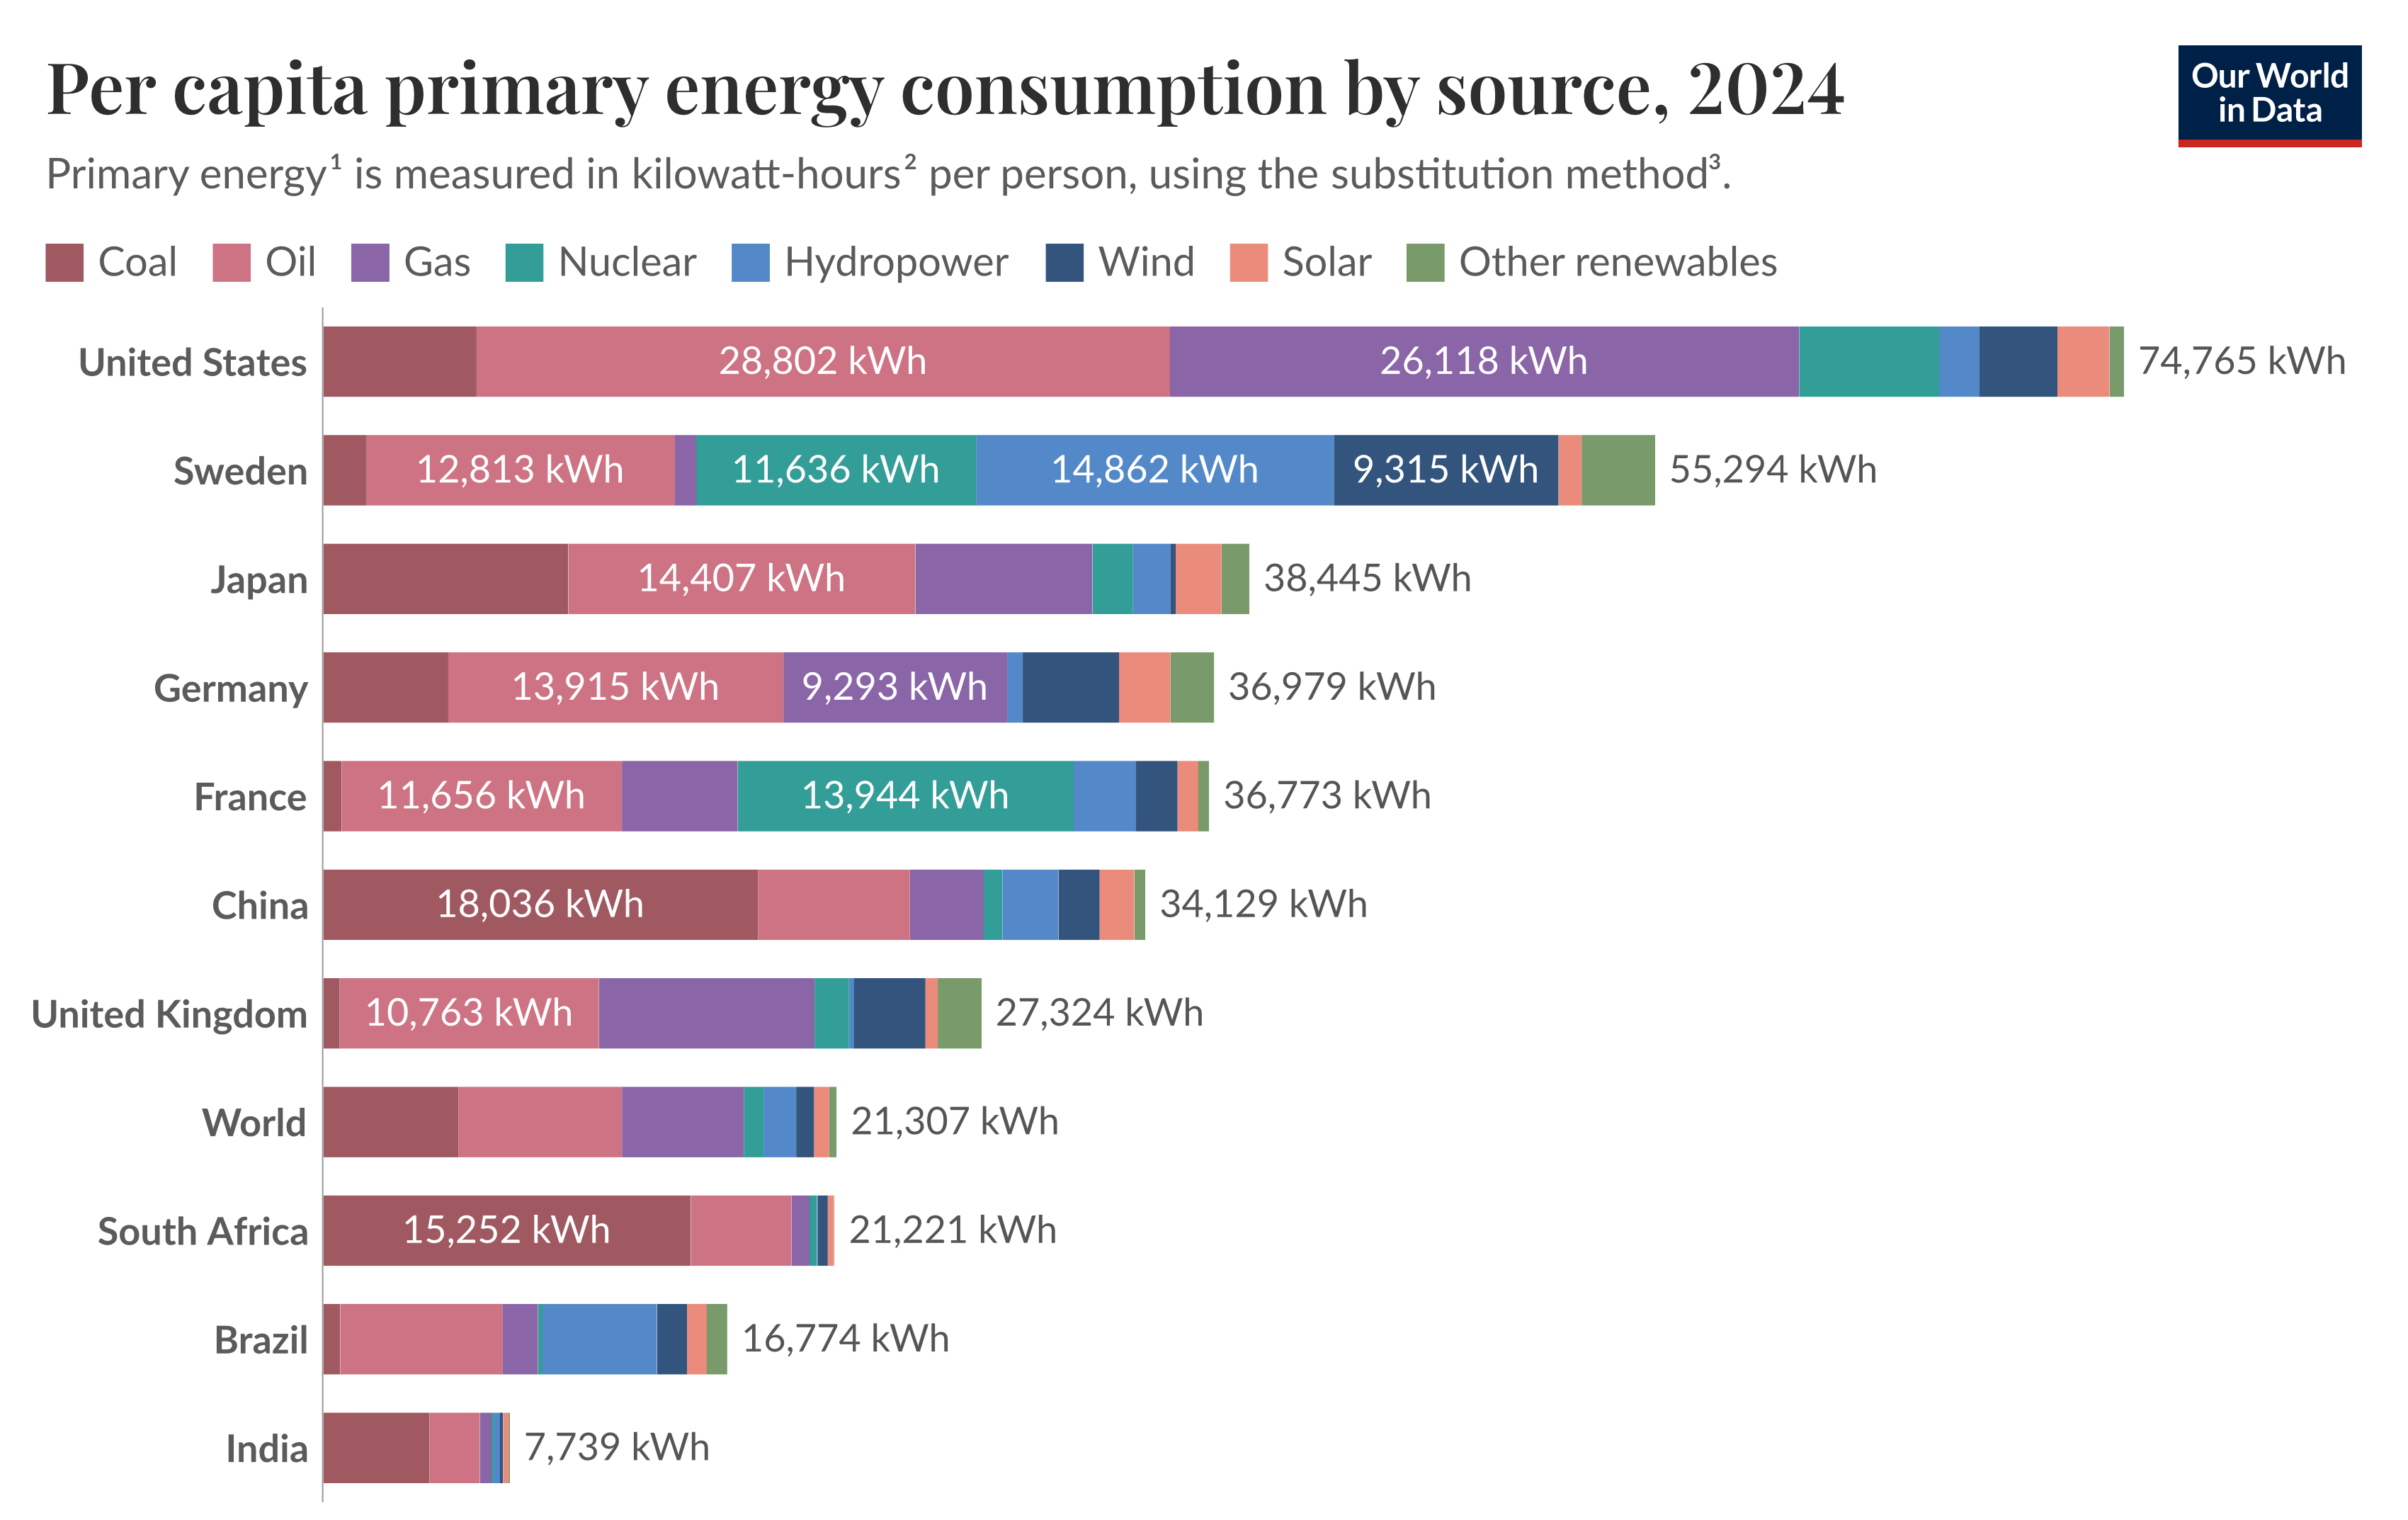
\includegraphics[width=\linewidth]{figures/per-capita-energy-stacked.png}
    \caption{Global primary energy consumption by source in 2024; source: \href{https://ourworldindata.org/energy-production-consumption}{Our World In Data}}
    \label{fig:energy_consumption_2024_percapita}
\end{figure}

Figure \ref{fig:energy_consumption_2024_percapita} presents the global primary energy use per capita in 2024 \cite{EnergyUsePerson}. Primary energy refers to energy in its raw, untransformed state, as extracted from natural resources. This includes, for example, coal prior to combustion, crude oil before refining, natural gas before processing, and uranium before enrichment\footnote{Following \href{https://ourworldindata.org}{Our World In Data}'s definition \cite{ritchieEnergyMix2020}, primary energy encompasses the total energy content of energy resources before conversion into secondary forms such as electricity, district heat, or refined fuels. It therefore includes both the energy ultimately delivered to end users and the losses and inefficiencies associated with transformation, transmission, and distribution processes.}.

Historical data indicate that global primary energy consumption has increased almost continuously over the past five decades, as shown in \Cref{fig:energy_trend_per_captia}. Notable exceptions include temporary declines in the early 1980s, during the global financial crisis in 2009, and in 2020 as a result of the COVID-19 pandemic. Although total energy consumption continues to rise, the growth rate appears to be stagnating, currently averaging approximately 1–2\% per year.

\begin{figure}[ht]
    \centering
    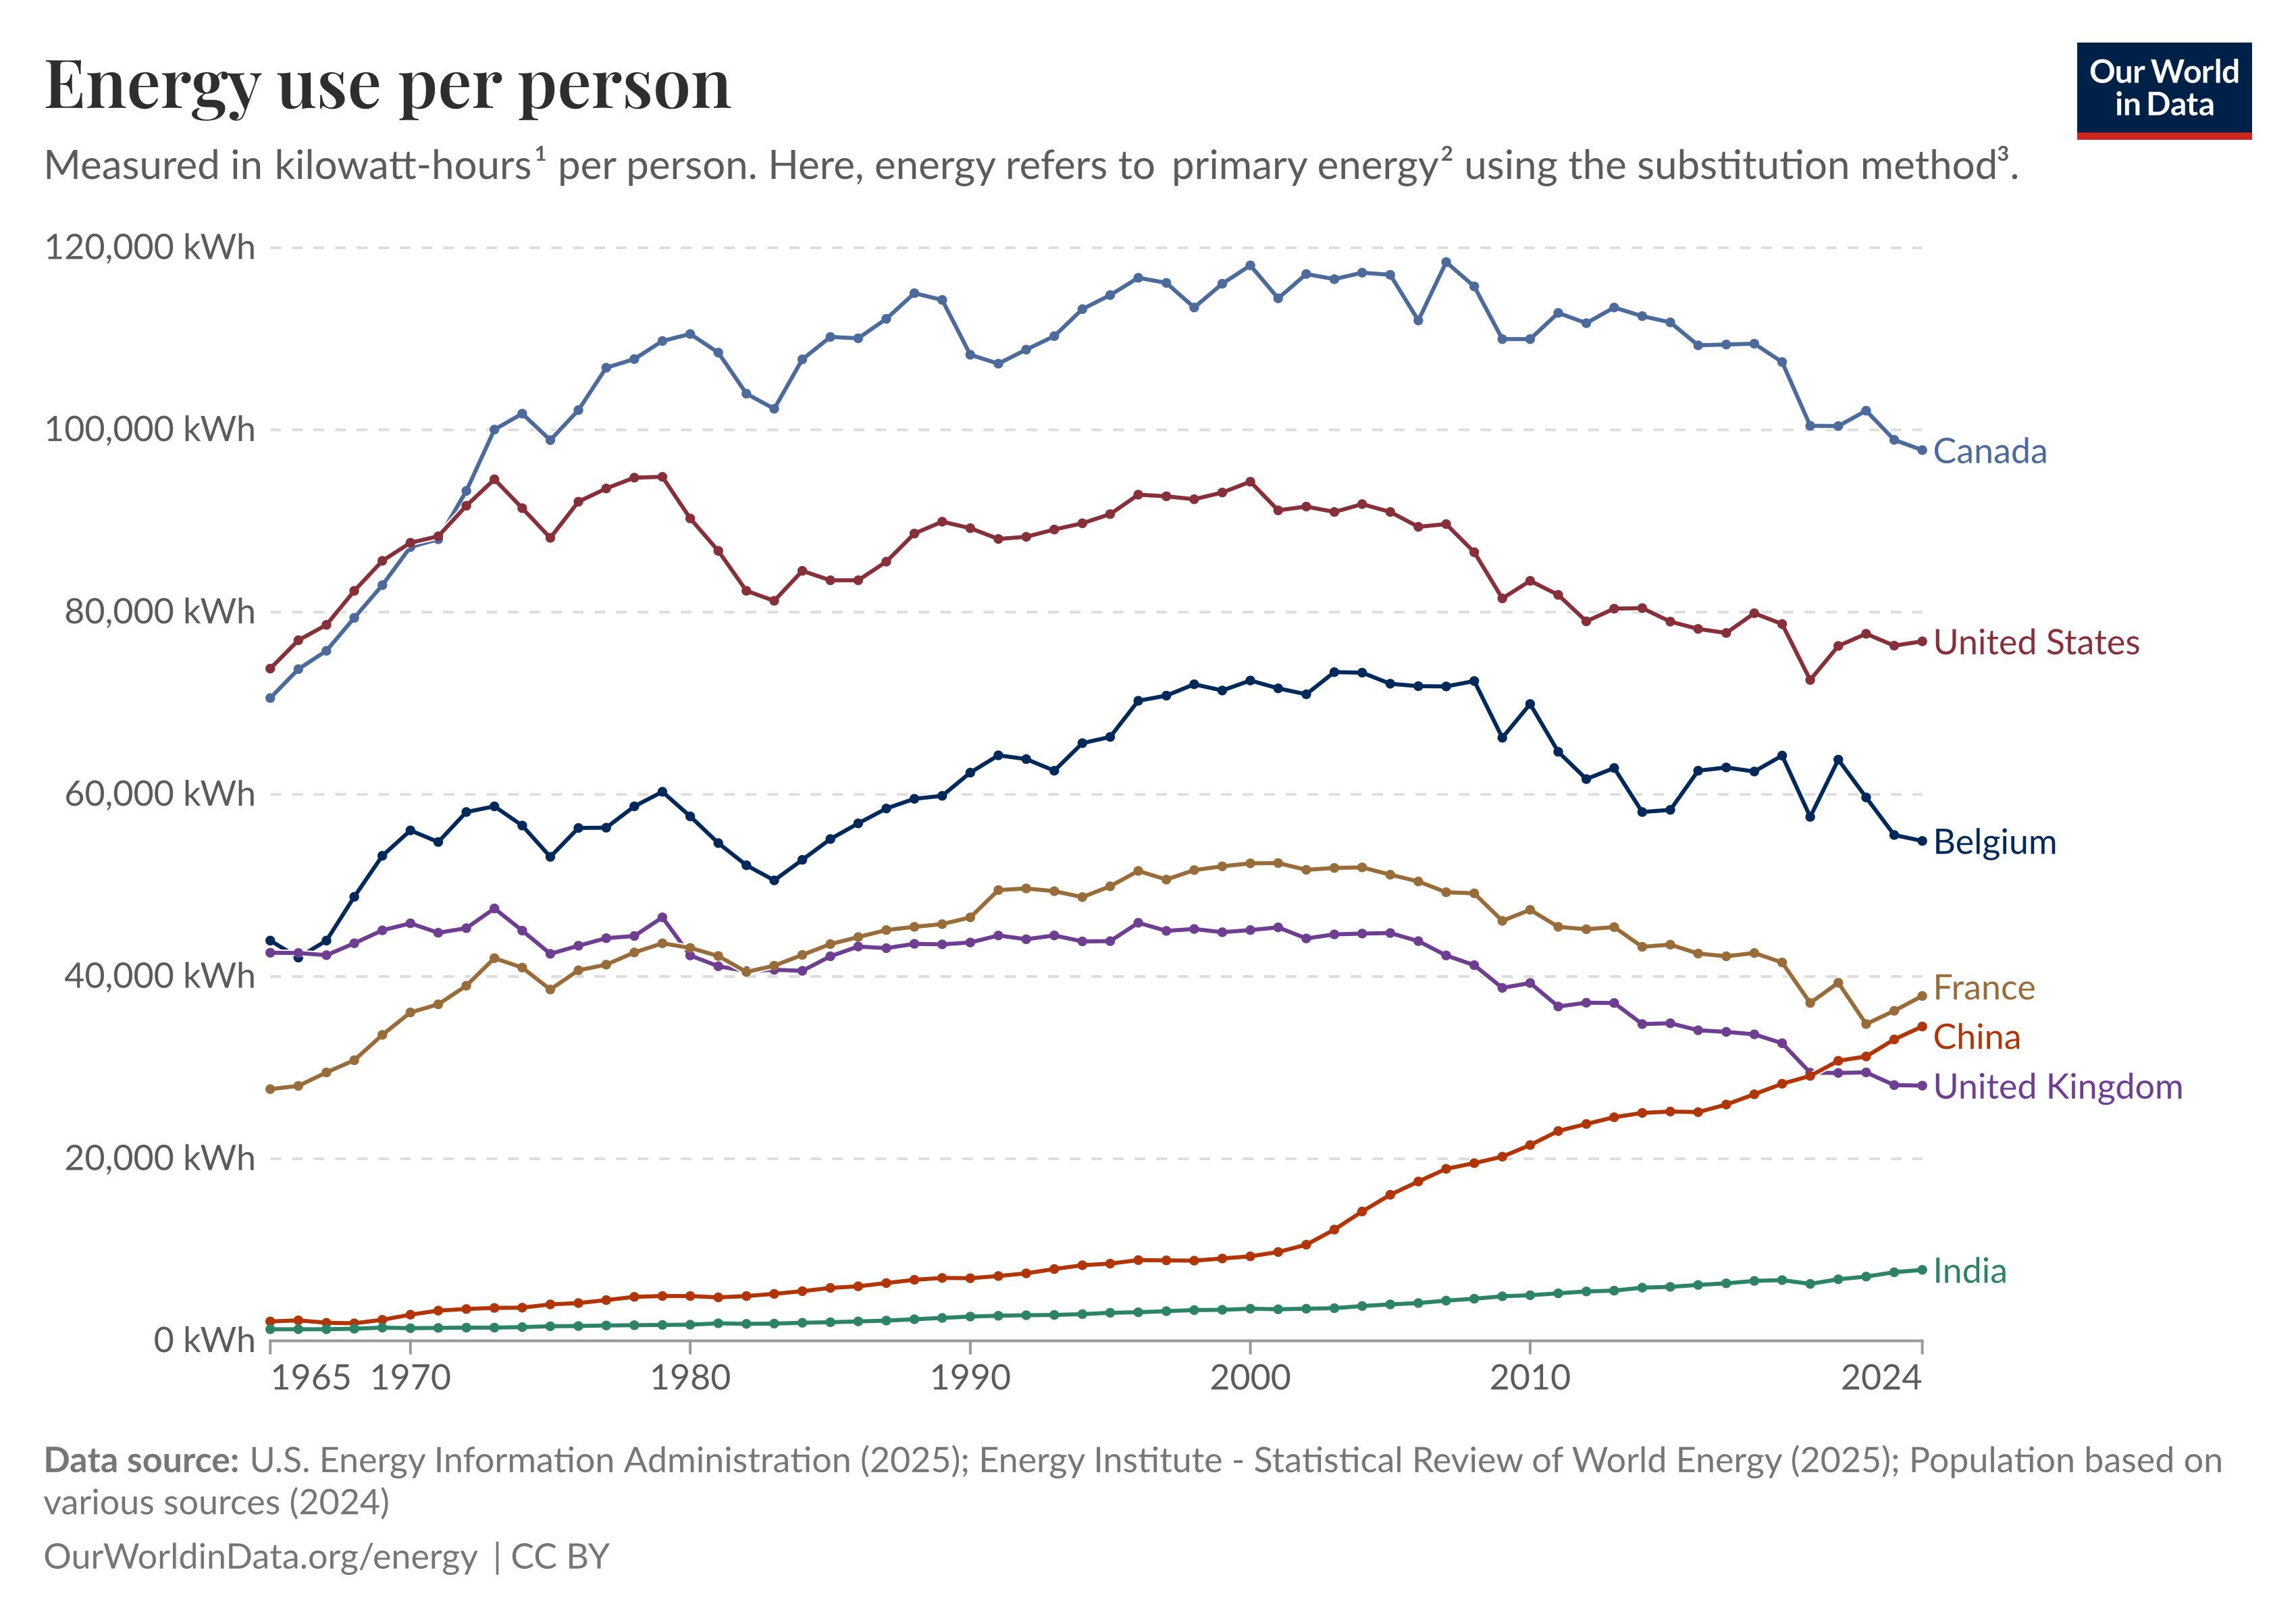
\includegraphics[width=0.8\linewidth]{figures/per-capita-energy-use-2.png}
    \caption{Per capita share of energy in 2024; source: \href{https://ourworldindata.org/energy-production-consumption}{Our World In Data}}
    \label{fig:energy_trend_per_captia}
\end{figure}
Overall, these trends reflect a structural increase in global energy demand, largely driven by population growth, economic \& technological development, and rising living standards in many regions. From an engineering perspective, this sustained demand growth reinforces the importance of designing energy systems that are not only efficient and reliable, but also sustainable and resilient in the context of climate and resource constraints.

% Energy is the fundamental ability to do work. We all need energy. Energy is increasingly becoming an important topic of discussion, in part due to the energy transition, but also due to the growing energy consumption.
% Cref{fig:x} shows the primary energy use per person in the world in 2024. The primary energy use refers. (World data defines primary energy as the energy that is available as resources – such as the fuels burnt in power plants – before it has been transformed. This relates to the coal before it has been burned, the uranium before it has been refined, or the barrels of oil before it has been processed. Primary energy includes energy that the end user needs, in the form of electricity, transport and heating, plus inefficiencies and energy that is lost when raw resources are transformed into a usable form.) (cite{world data}. We see that global energy consumption has increased nearly every year for more than half a century. The exceptions to this are in the early 1980s, 2009 following the financial crisis, and 2020 due to the COVID-19 pandemic.
% Global energy consumption continues to grow, but the growth does seem to be slowing down—averaging around 1\% to 2\% per year.
% Thus, we see that the demand for energy is growing across many countries in the world, as people get richer and populations increase.

\subsection{Energy Mix}
Figure \ref{fig:global_energy_shares} illustrates the global distribution of primary energy consumption by source and shows a rapid increase in energy consumption from the 20th century onwards. Oil remains the dominant contributor to the global energy mix, followed by coal and natural gas, with hydroelectric power representing a smaller but still significant share. Although modern renewable energy sources (\hyperref[sec:renewable_energy]{RES})—such as wind and solar—currently account for a comparatively modest fraction of total primary energy use, their growth rates over the past decade have been substantial.

% From ref{fig} we see that globally we get the largest amount of our energy from oil, followed by coal, gas, and hydroelectric power. Although renewable make for a very small amount compared to the other energy sources, they are now growing quickly. Ref{fig} shows a chart with the specific breakdown by source, including coal, gas, oil, nuclear, hydro, solar, wind, and other renewables (which include bioenergy, wave, and tidal). This is given in terms of per capita consumption. Here it is also clear that global trends tend towards the same conclusion: energy demand is rising.

\begin{figure}[ht]
    \centering
    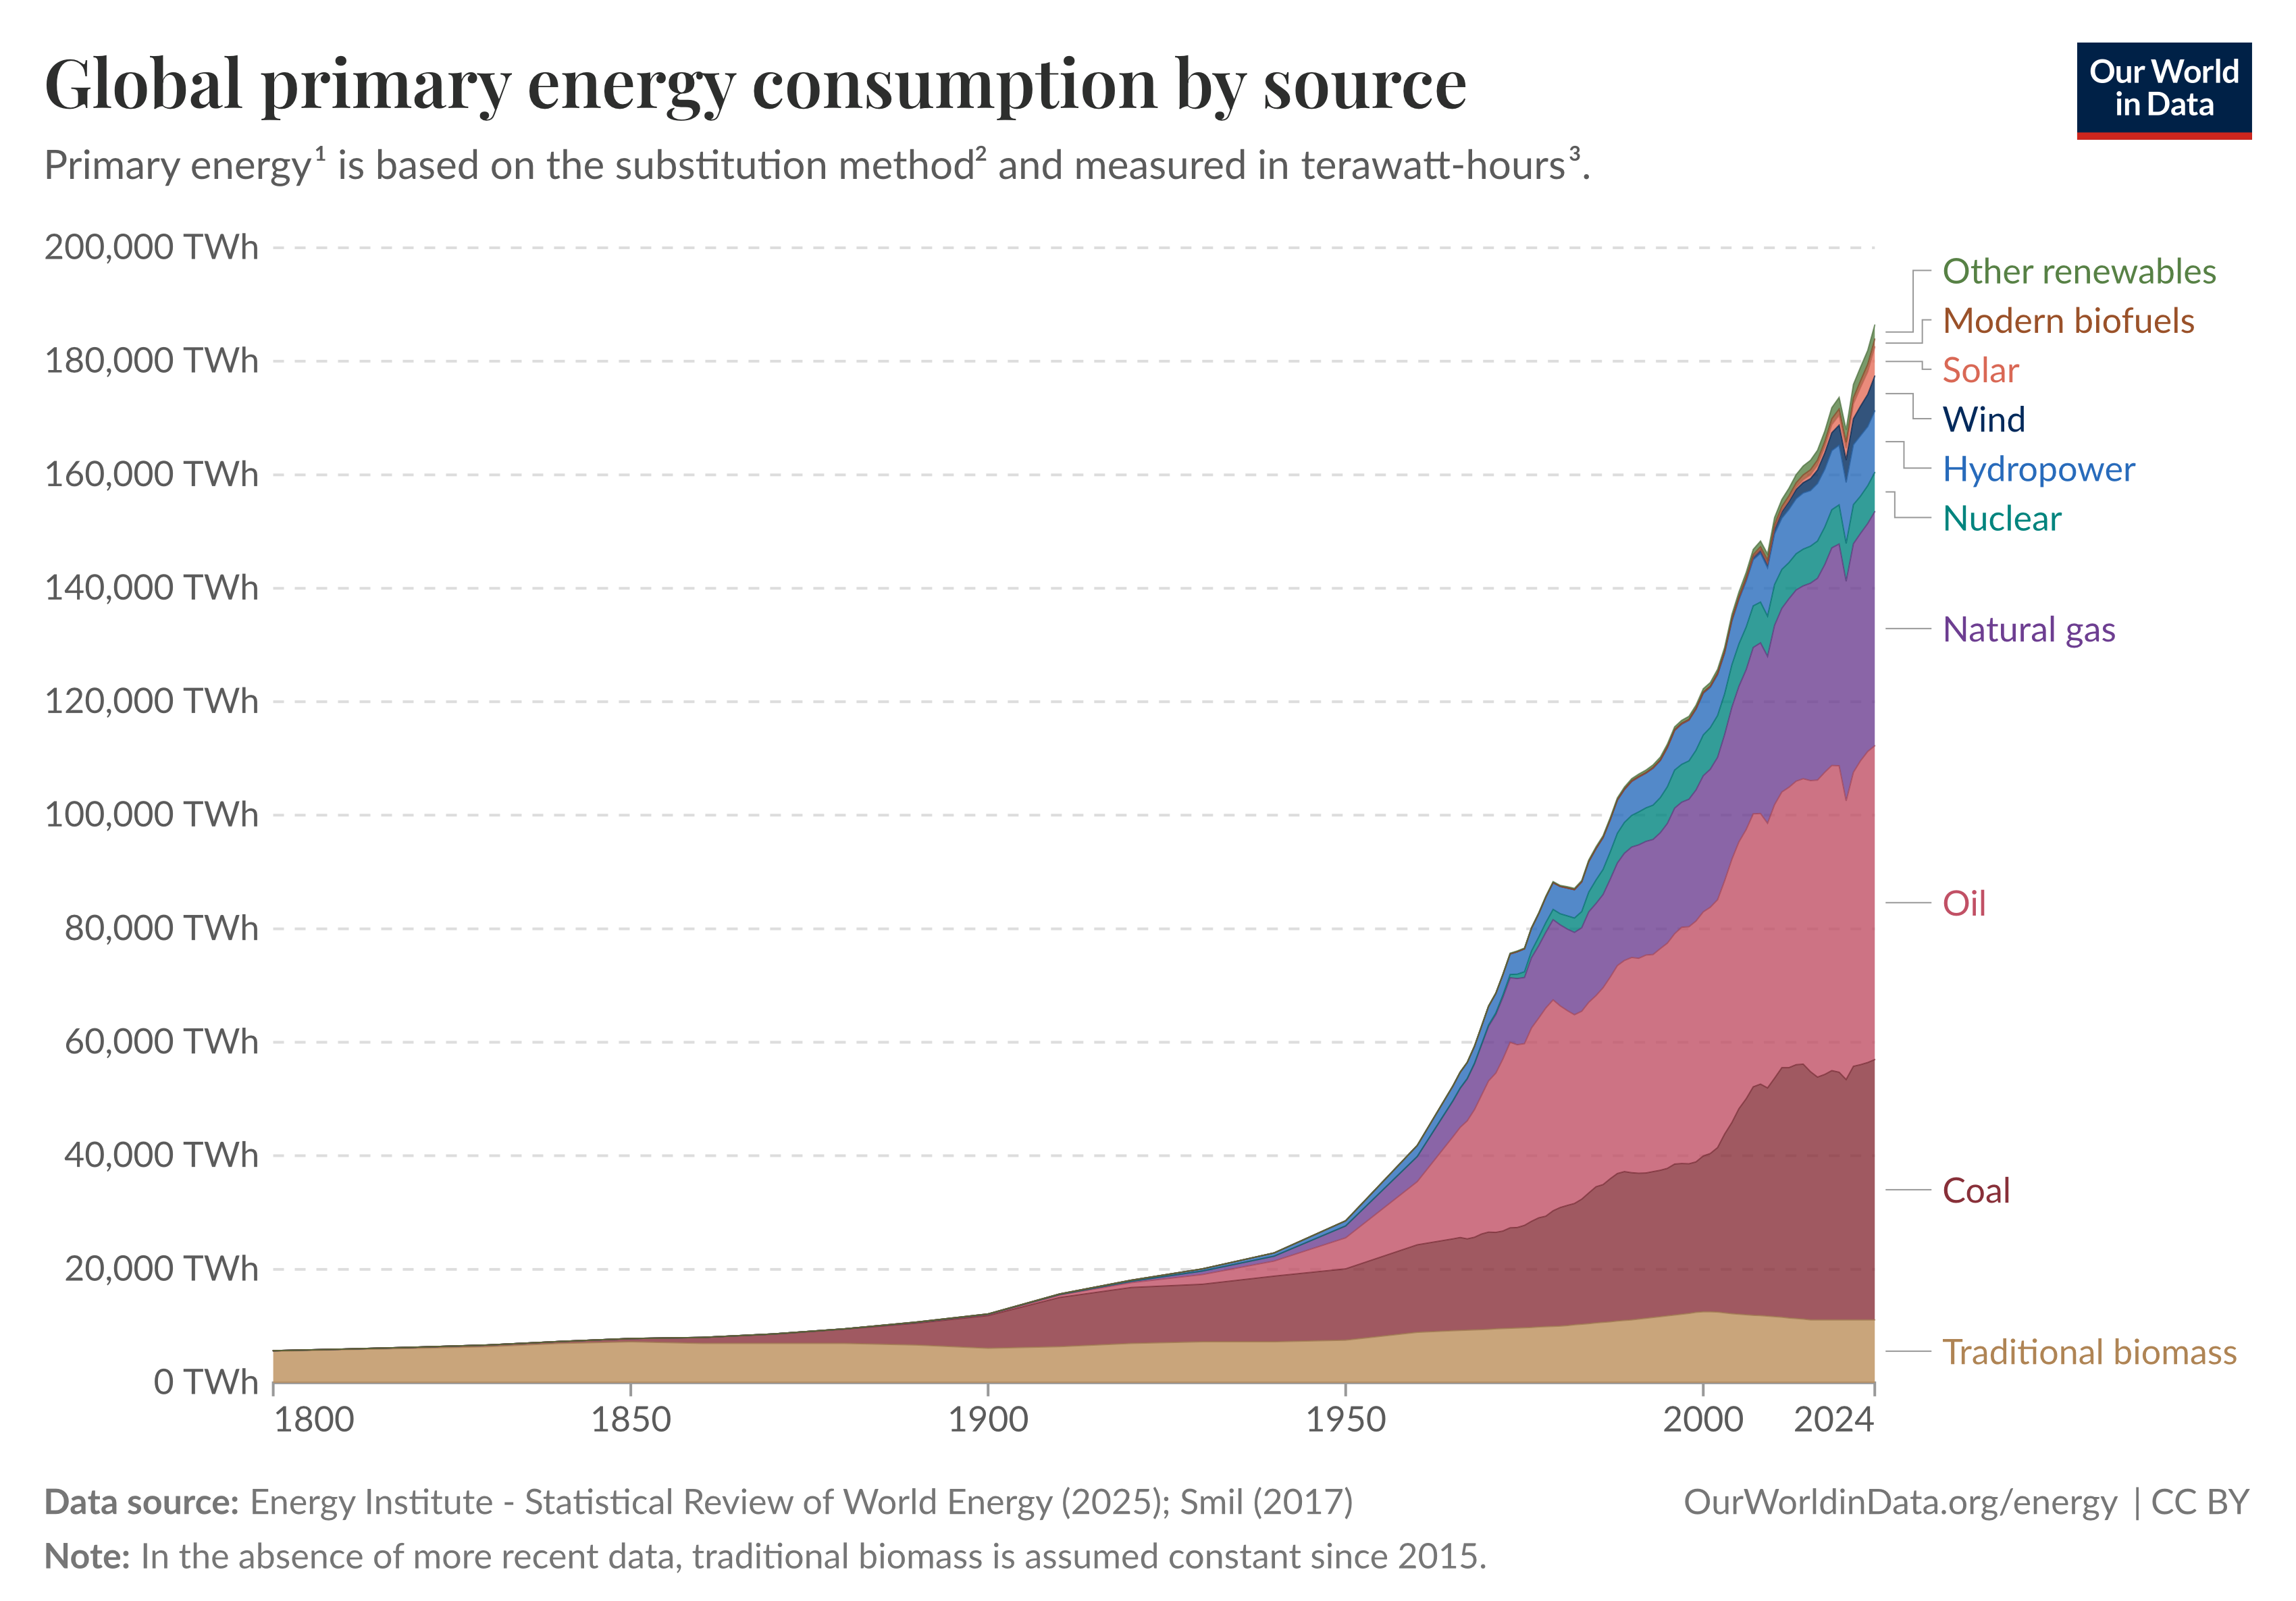
\includegraphics[width=0.85\linewidth]{figures/global-energy-substitution.png}
    \caption{Different sources of global energy use over the years; source: \href{https://ourworldindata.org/energy-mix}{Our World In Data}}
    \label{fig:global_energy_shares}
\end{figure}


\subsection{Electricity Mix}\label{sec:electricity_mix}
The electricity mix constitutes a specific subset of the broader energy mix. While the overall energy mix includes all primary energy uses—such as transport fuels, industrial heat, and residential heating—the electricity mix refers exclusively to the energy sources used to generate electrical power. In other words, it represents the composition of fuels and technologies that supply the grid and ultimately power households, industry, digital infrastructure, and electric vehicles (EVs) \cite{EnergyMix2025}. Consequently, the relative shares of coal, oil, natural gas, nuclear energy, and renewable sources differ between the total energy mix and the electricity mix.

The line chart in Figure \ref{fig:elec_mix_share_by_source} illustrates the evolution of each source’s share in global electricity generation over time. Globally, coal remains the dominant source of electricity generation, followed by natural gas. Among low-carbon sources, hydropower and nuclear energy historically contribute the largest shares, although wind and solar power have experienced rapid growth in recent years and are increasingly significant contributors to new capacity additions \cite{RenewableElectricityRenewables}.

\begin{figure}[ht]
    \centering
    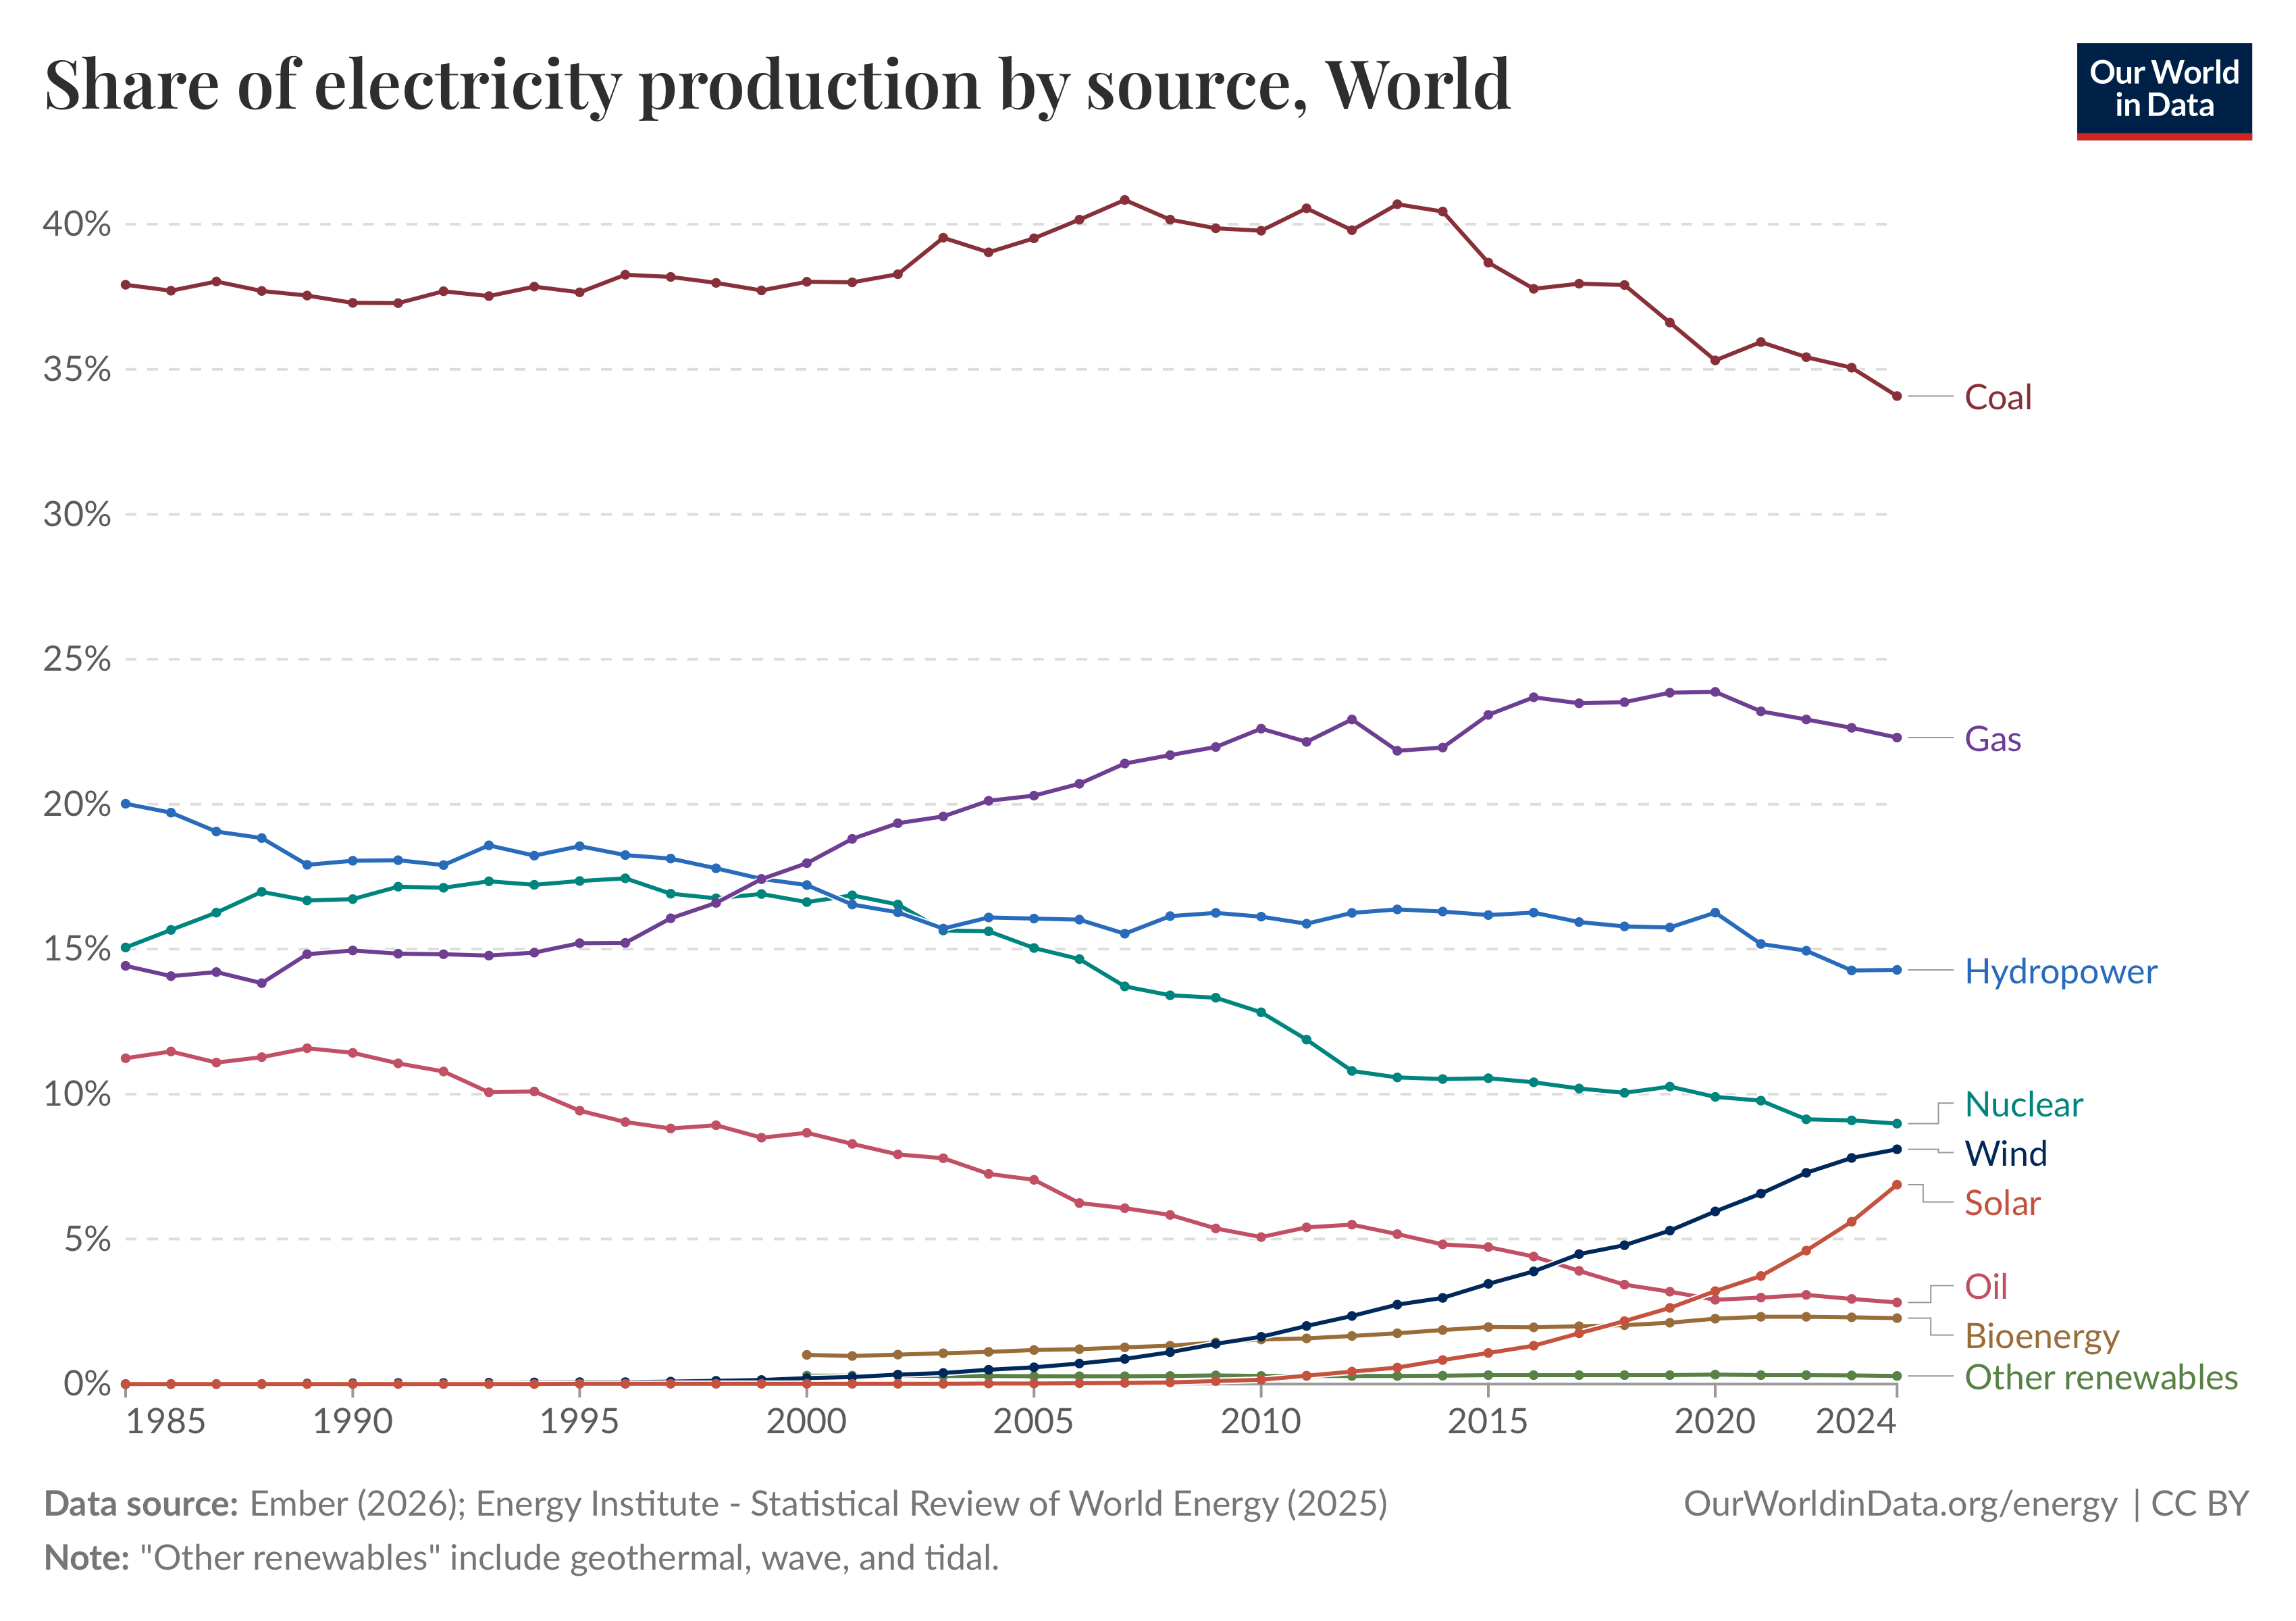
\includegraphics[width=0.7\linewidth]{figures/share-elec-by-source.png}
    \caption{Different shares of electricity production by source throughout time; source: \href{https://ourworldindata.org/electricity-mix}{Our World In Data}}
    \label{fig:elec_mix_share_by_source}
\end{figure}

\subsubsection*{Belgian electricity mix}
The Belgian electricity mix exhibits a markedly different structure. As shown in Figure \ref{fig:BE_elec_share}, approximately 28\% of electricity generation is derived from fossil fuels, while around 33\% originates from nuclear power. RES—particularly wind and solar—account for a substantial and growing share of generation. This national profile reflects how electricity mixes can vary significantly across countries despite similar overarching decarbonization objectives.

\begin{figure}[ht]
    \centering
    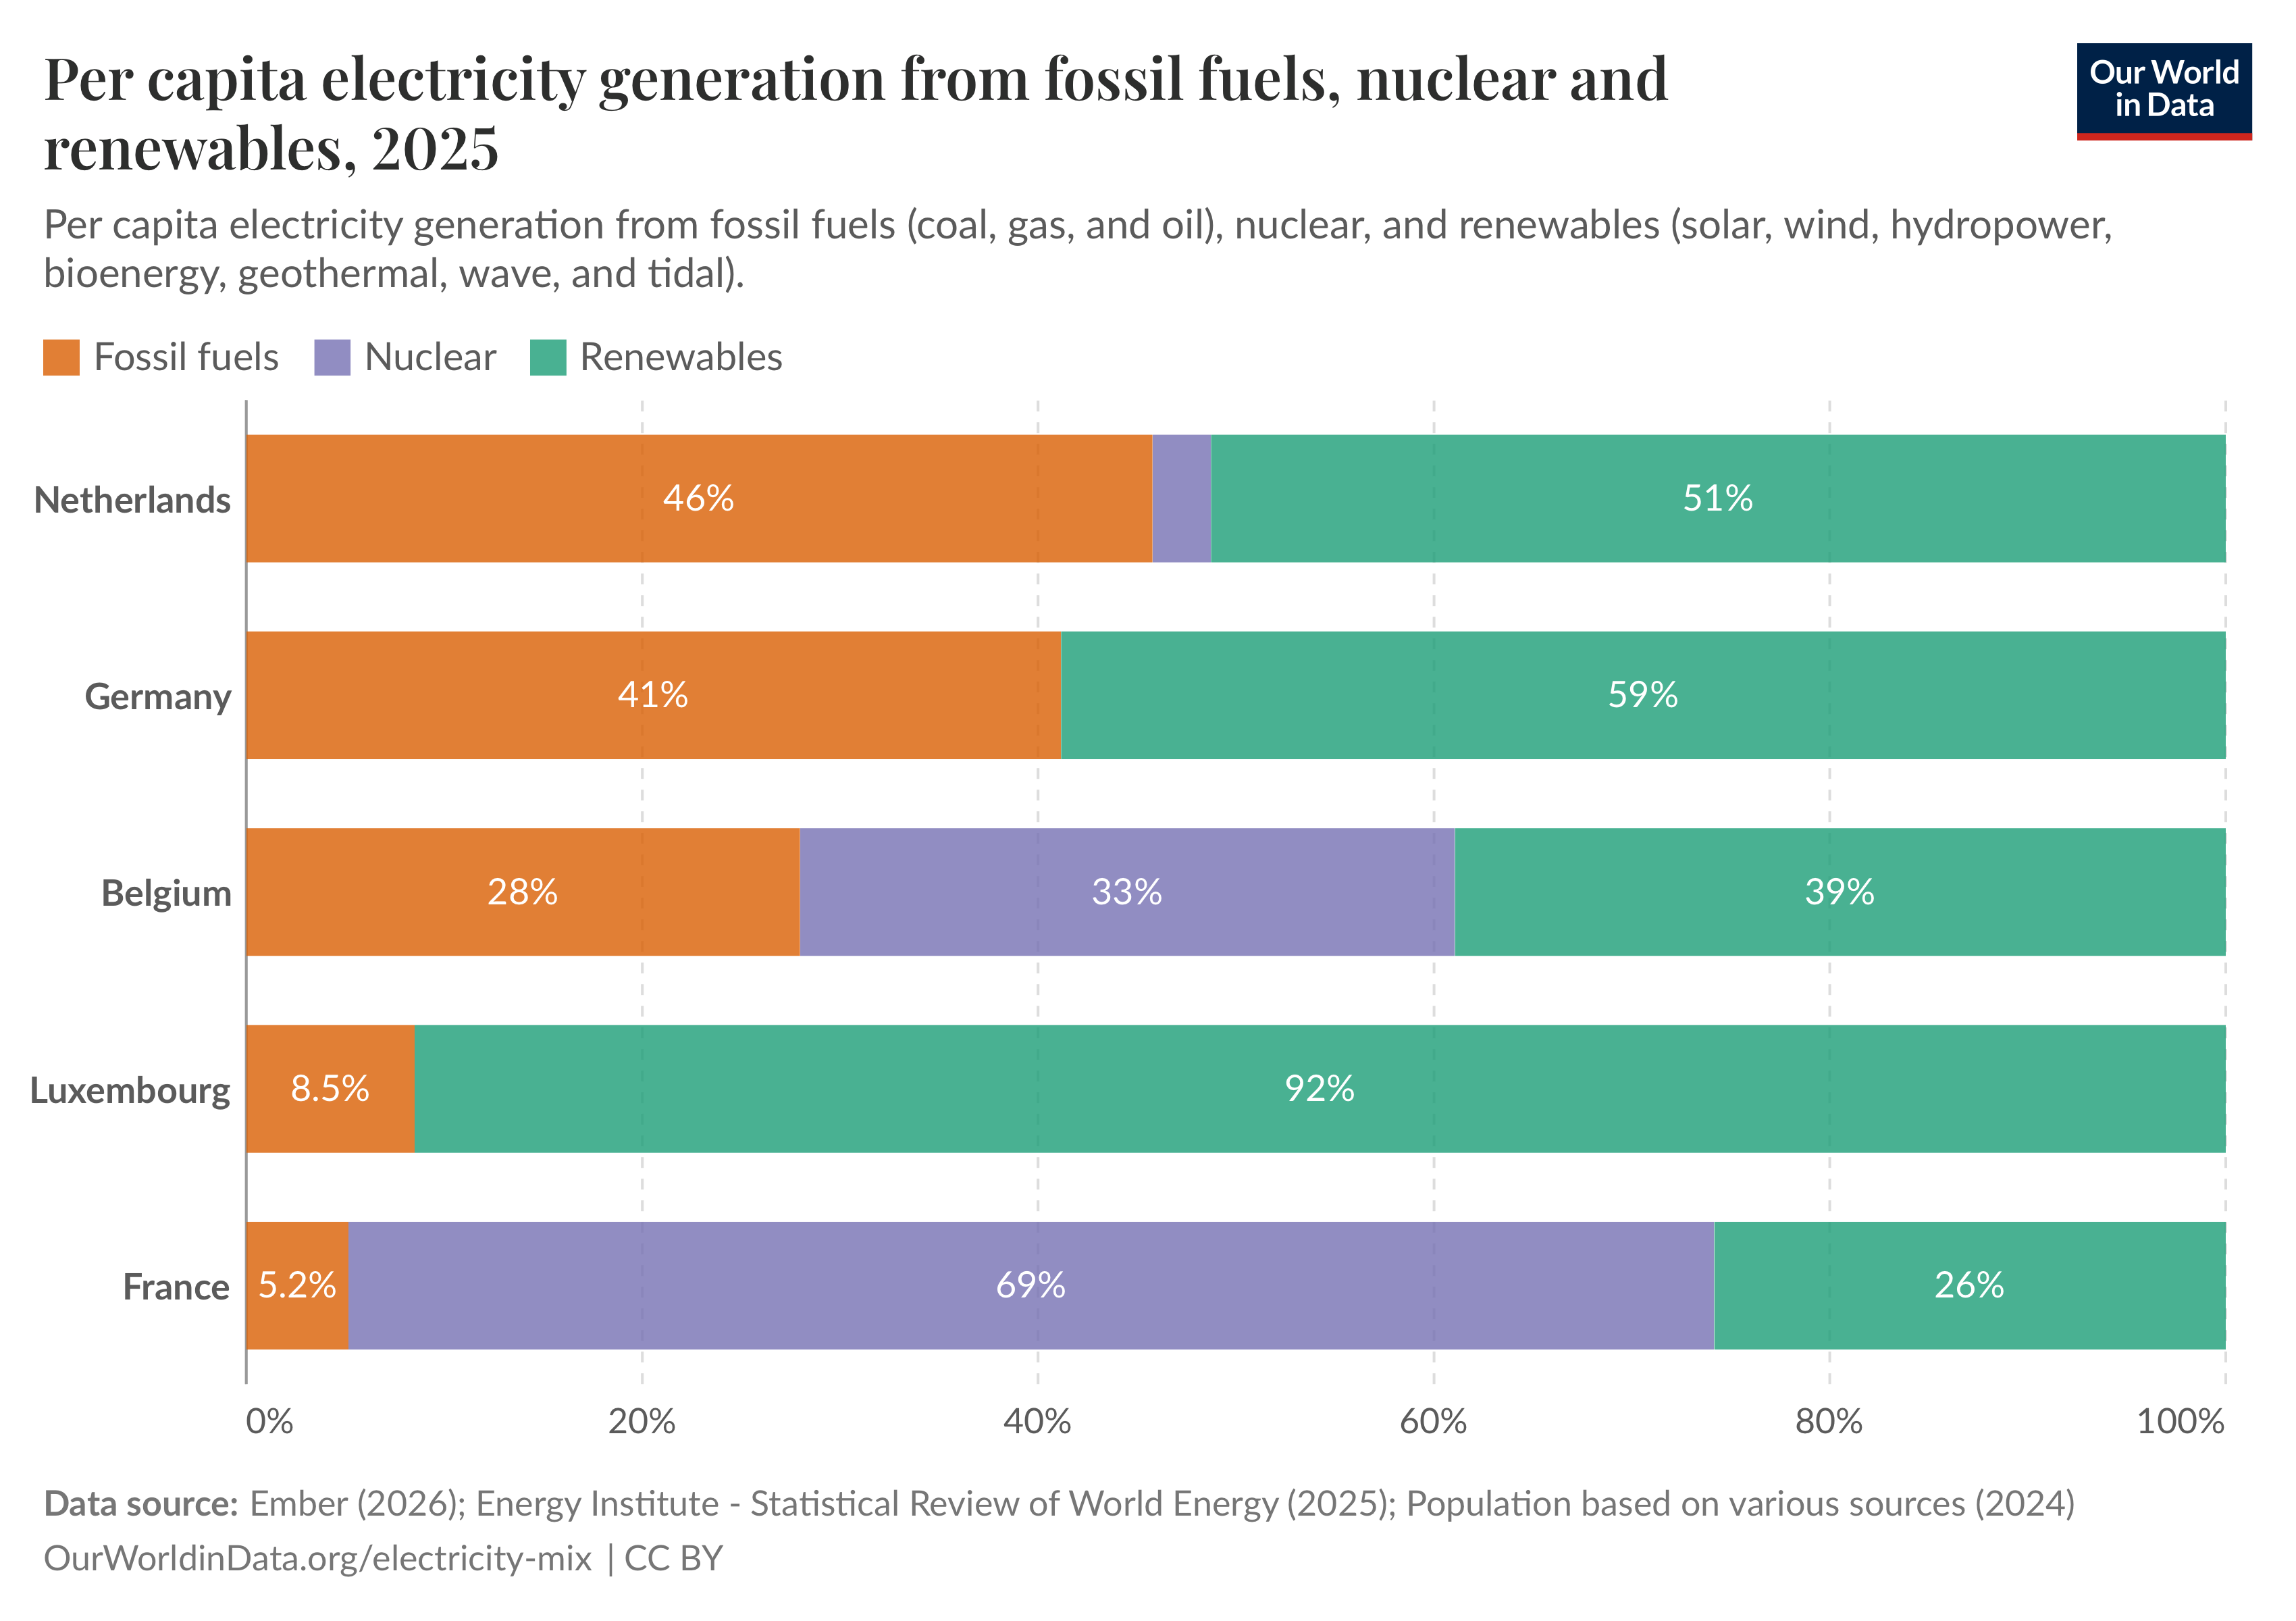
\includegraphics[width=0.8\linewidth]{figures/per-capita-electricity-fossil-nuclear-renewables.png}
    \caption{Share of electricity in Belgium compared to the neighbouring countries; source: \href{https://ourworldindata.org/electricity-mix}{Our World in Data}}
    \label{fig:BE_elec_share}
\end{figure}


\subsection{Renewable Energy}\label{sec:renewable_energy}
Renewable energy is power generated from natural sources that replenish on a human timescale, such as the sun, the wind, water, and heat from the earth. These sources are used to produce electricity and heat with significantly lower greenhouse gas (GHG) emissions\footnote{The \href{https://www.ipcc.ch}{IPCC} formally describes GHG emissions as gaseous components of the atmosphere that absorb and emit radiation at specific wavelengths within the spectrum of radiation emitted by the Earth’s surface, by the atmosphere itself, and by clouds. This traps heat, keeps the earth warm, and is called the greenhouse effect \cite{FrequentlyAskedQuestions}.} compared to fossil fuels, making them vital for addressing climate change and air pollution \cite{RenewableEnergyEESI}.

\subsubsection*{Technology \& deployment}
Common technologies include photovoltaic (PV) panels, wind turbines, water dams, and geothermal heat pumps. \Cref{fig:conversion_techs} shows a summary of those technologies paired with their possible energy sources. The main technologies studied for this thesis are PV panels and heat pumps, as they are the most relevant to the scope of residential energy modelling (\Cref{sec:residentialTechnologies}).

\begin{figure}[ht]
    \centering
    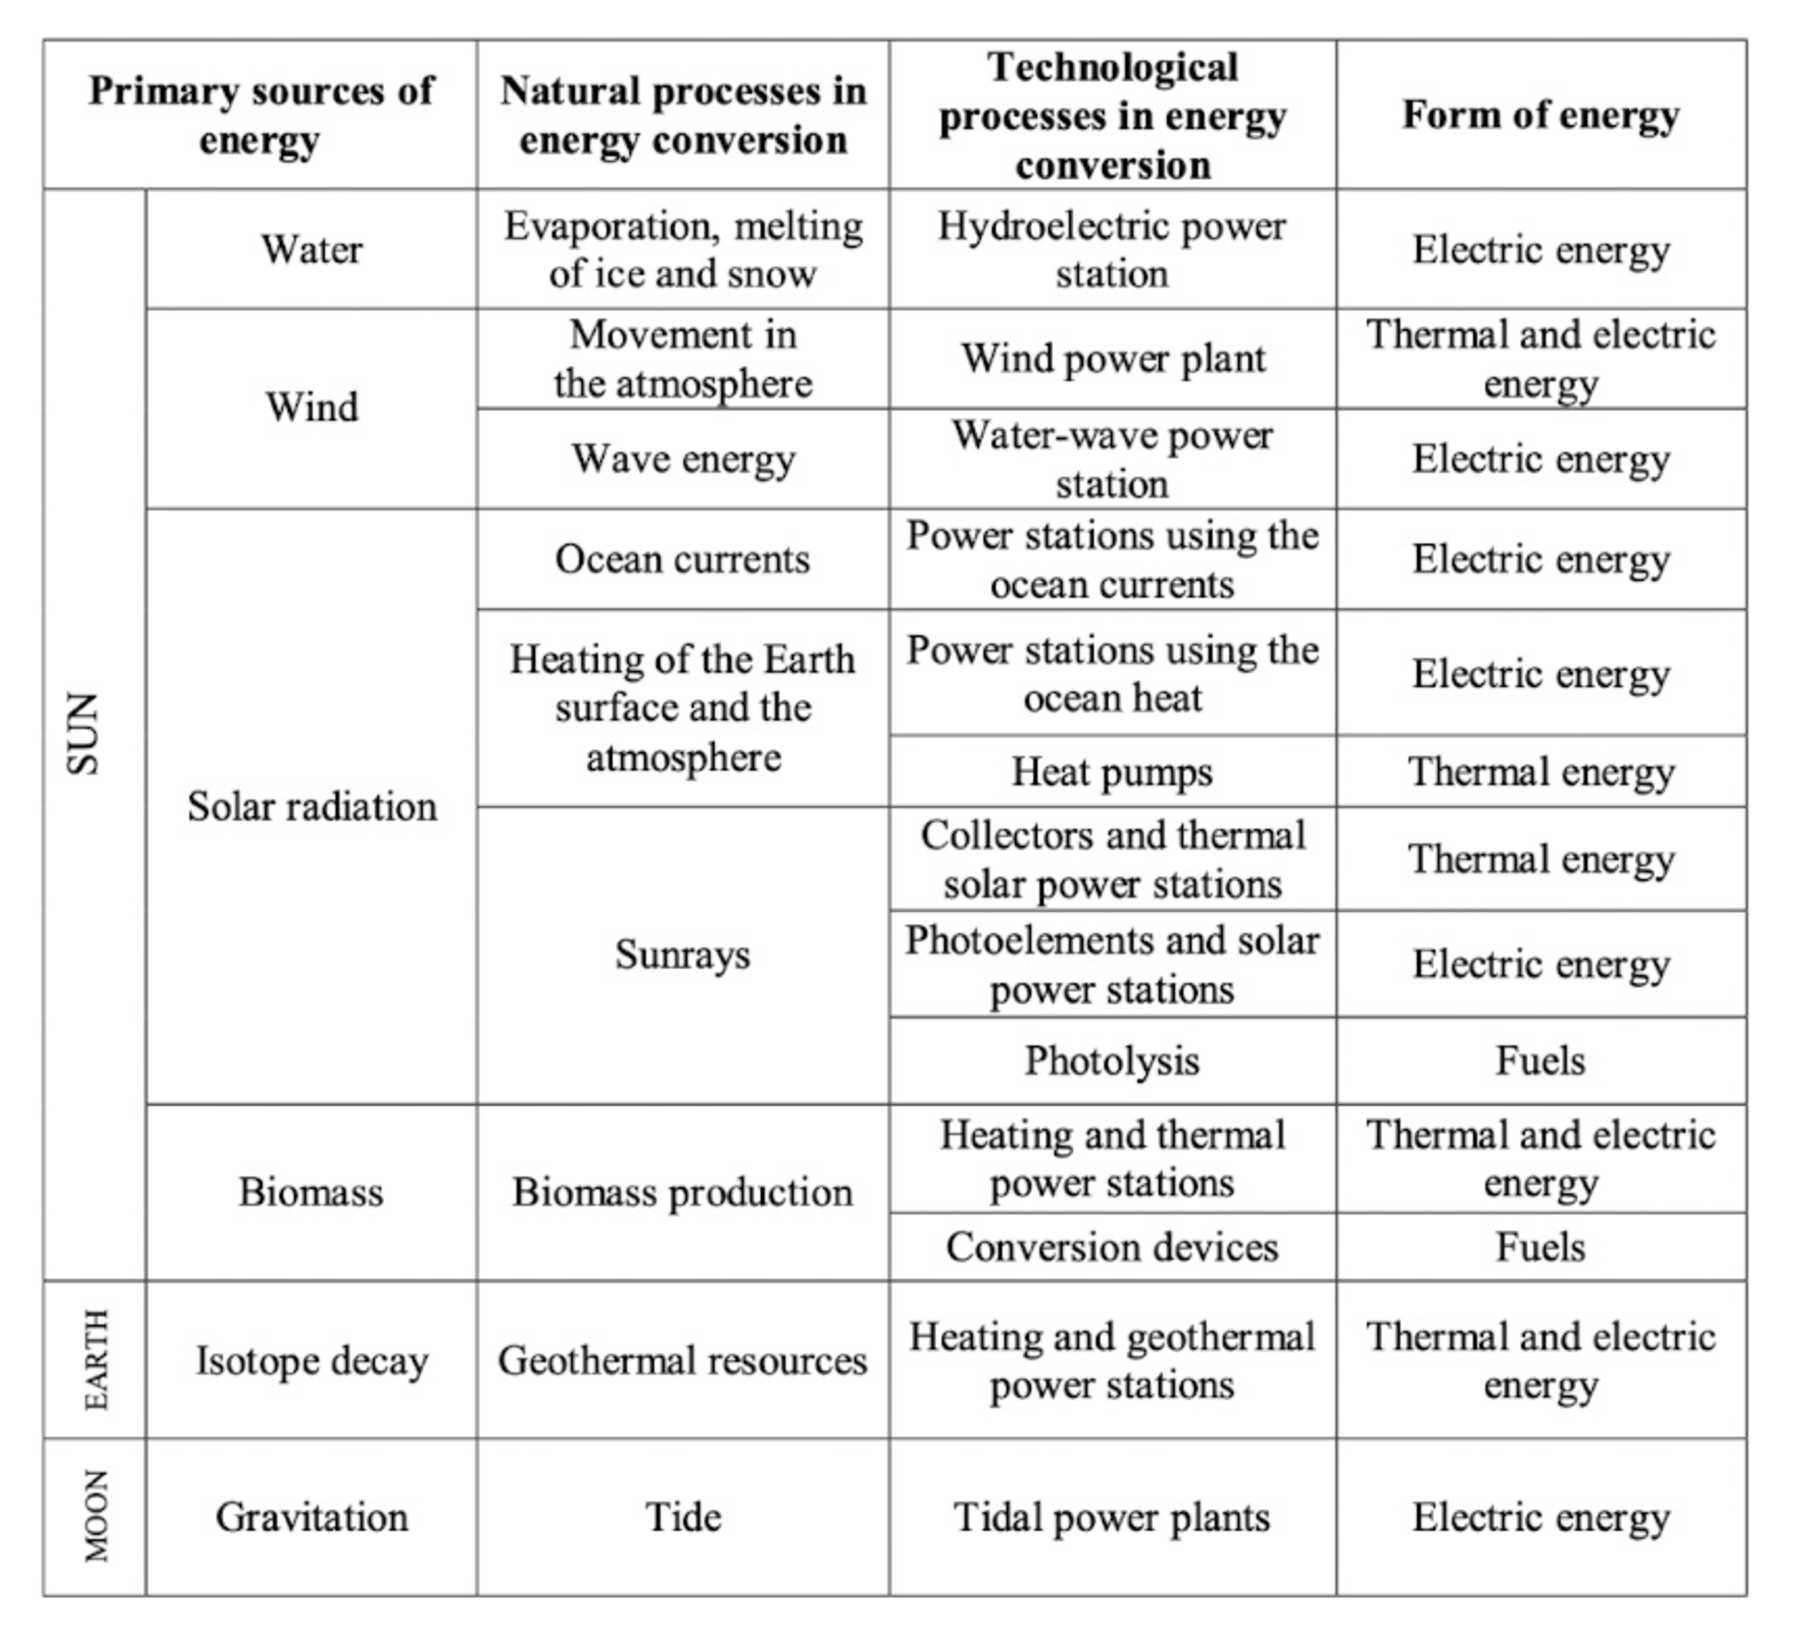
\includegraphics[width=0.8\linewidth]{figures/conversion_tech.pdf}
    \caption{Division of renewable energy sources and the possibilities of conversion, adapted from Zielińska~\cite{zielinska2010_sustainable_development} by Prof. Svend Bram.}
    \label{fig:conversion_techs}
\end{figure}

\subsubsection*{Sustainability}
Renewables are closely linked to sustainable energy—but they are not quite the same thing. The term ``sustainability'' refers to a society's ability to exist, develop, and meet the needs of the present without compromising the ability of future generations to meet their own needs and develop. Sustainability goes further than only the energy supply. It includes environmental, economic and social dimensions. 

\subsubsection*{Decarbonisation}
The relevance of renewable energy follows directly from the energy system's dominant role in global warming: roughly 73\% of global anthropogenic GHG emissions originate from energy production and use \cite{intergovernmentalpanelonclimatechangeipccEnergySystems2023}. Any credible mitigation strategy must therefore target the decarbonisation of energy systems first.
\newline Renewable technologies meet this challenge by replacing carbon-intensive carriers with low- or zero-emission alternatives. Solar and wind generate electricity without combustion-related emissions, while hydropower and geothermal provide relatively stable low-carbon supply. Raising the renewable share is thus a necessary condition for reducing emissions at scale—the rationale underpinning frameworks such as the European Green Deal, which targets climate neutrality by 2050 through a large-scale transformation of the energy system \cite{EuropeanGreenDeal}.

\subsubsection*{Reduction \& reconstruction of energy demand}
The transition cannot be framed solely as expanding clean supply. Global energy demand is still rising—driven by population growth, economic development, and digitalisation—so renewables must both displace fossil generation and meet additional demand, sharply increasing the required deployment rate and system complexity \cite{ritchieEnergyMix2020}. This is the central limitation of a purely supply-driven view.
\newline Reducing and restructuring demand is therefore equally important. Lower total consumption shrinks the infrastructure needed for decarbonisation and eases pressure on resources, land use, and grid stability, while reshaping demand—through efficiency, behavioural change, and demand-side flexibility—improves alignment with variable generation. Better insulation cuts heating demand, and flexible consumption lets load follow renewable output, reducing the need for storage and balancing capacity. Demand reduction is, in this sense, a fundamental lever for making the transition technically and economically feasible.

\subsubsection*{Increasing RES}
Despite these challenges, renewable deployment has accelerated markedly. Although fossil fuels still dominate the primary energy mix, RES supplied roughly 8\% of global primary energy in 2023 and are projected to reach roughly 30\% of global primary energy by 2050 under current and announced policy trajectories \cite{iea2025weo}. This growth is driven mainly by falling wind and solar costs, supportive policy, and rising climate ambition at national and supranational levels.
\newline Integrating high RES shares generally requires a broader portfolio of balancing options—storage, transmission expansion, demand-side response, sector coupling, curtailment management, improved forecasting, synchronous condensers, and advanced inverter controls such as fast frequency response and grid-forming functionality. Robust electricity-demand modelling becomes correspondingly valuable: the better operators understand when, where, and how strongly demand evolves, the more effectively they can integrate renewable generation while preserving reliability and minimising curtailment and balancing costs \cite{entsoe_flexibility_res_2025, iea_value_demand_flexibility_2025}.

\paragraph{Merit order.} 
Variable RES reshapes power-system operation through the merit order. In liberalised markets, units are dispatched in ascending order of marginal cost \cite{PowerExchangeMarkets}; because wind and solar have near-zero marginal cost, they shift the merit order rightward, displacing costlier conventional plants and lowering wholesale prices when renewable output is high. This \textit{merit-order effect} cuts short-term system costs but compresses revenues for dispatchable generation, weakening investment signals for firm capacity.

\paragraph{Duck curve.} 
At higher penetration, the same dynamic produces sharp temporal mismatches between generation and demand, captured by the \textit{duck curve}: low net demand during midday solar peaks, followed by steep evening ramps as solar fades. System flexibility requirements rise accordingly, calling for fast-response generation and storage.

\subsubsection*{Renewables--pros \& cons}
The expansion of renewable energy thus presents a set of structurally coupled advantages and challenges. On the one hand, RES enable deep decarbonisation, reduce marginal generation costs, and decrease dependence on imported fuels. On the other hand, their variability introduces operational complexity, including increased balancing requirements, price volatility, and potential adequacy concerns due to reduced revenues for dispatchable generation. These trade-offs do not represent fundamental limitations, but rather a shift in system design requirements—from fuel-based optimisation toward flexibility, coordination, and temporal alignment between supply and demand.

\subsubsection*{Renewables in Belgium}
The Belgian electricity mix, as shown earlier in Figure \ref{fig:BE_elec_share}, reflects both progress and structural constraints. While the share of renewable energy remains modest in absolute terms compared to some frontrunner countries, Belgium performs relatively well within its regional context. Neighbouring countries exhibit varying profiles: Germany and the Netherlands rely more heavily on fossil fuels alongside expanding renewable capacity, whereas France derives the majority of its electricity from nuclear power. Belgium’s energy system shares certain similarities with France in that nuclear energy has historically played a significant role in electricity generation \cite{NuclearPowerBelgium}. Figure \ref{fig:BE_elec_share} shows that in 2025, nuclear power accounted for approximately 33\% of Belgium’s electricity mix. Nevertheless, public concerns regarding nuclear safety and long-term waste management, combined with evolving policy decisions, have led to a gradual phase-out strategy\footnote{In recent years, five of Belgium’s seven nuclear reactor units have been decommissioned following increasingly stringent regulatory and political measures \cite{NuclearPowerBelgium}.} 

\subsubsection*{Is nuclear power sustainable?}
Nuclear energy is released from the atomic nucleus. Today's nuclear electricity is produced by fission, which harnesses the energy from splitting heavy nuclei to raise steam and drive a turbine\footnote{Electricity can also be generated by nuclear fusion, but this remains at the research stage \cite{WhatNuclearFusion2023}.}. It is not renewable, since it depends on a finite supply of uranium rather than a source replenished on a human timescale. Its sustainability is contested. Proponents and major bodies such as the IAEA present nuclear as a pillar of a sustainable future, citing its low-carbon life cycle and high energy density \cite{FiveReasonsClean2026}. Critics, including CAN Europe, argue it fails the criteria for a sustainable source given unresolved waste management and the environmental burden of resource extraction \cite{c.dascaluPOSITIONPAPERNuclear2024}. New projects are also notoriously slow (10–15 years) and expensive \cite{StorageDisposalRadioactive, CanNuclearPower}, which critics see as a poor fit for urgent 2030 targets relative to rapidly deployable renewables. Even so, nuclear is increasingly classified as sustainable within modern climate-policy frameworks: the EU taxonomy now lists it as a ``transitional'' sustainable activity, provided projects meet strict safety and waste-disposal standards \cite{EUTaxonomySustainable}.

\subsubsection*{Socio-political challenges}
While the technical feasibility of highly renewable electricity systems is well supported, the primary barriers to implementation are increasingly recognised as socio-political rather than engineering-related. Large-scale deployment of wind farms, solar parks, and transmission networks is often constrained by permitting delays, land-use conflicts, and public acceptance, reflecting competing interests around environmental protection, landscape aesthetics, and local community concerns. The transition is therefore governed not only by technological readiness but also by institutional capacity and governance structures \cite{IEA_NetZero2021, WorldBank_Minerals2020}.
\newline It also requires substantial restructuring of electricity markets and policy frameworks. High shares of variable renewables demand new mechanisms for valuing flexibility, adequacy, and system services that traditional market designs do not fully capture, while coordinating investment in transmission, storage, and demand-side flexibility adds complexity and requires long-term policy consistency. Decarbonisation is thus best understood as a socio-technical transformation, in which engineering solutions must be embedded within politically and socially viable pathways \cite{IEA_NetZero2021}.

\subsubsection*{Achieving 100\% renewable}
Substantial modelling shows that renewable-dominated electricity systems can, in principle, reach high reliability and adequacy \cite{Denholm2021, Brown2018, Zappa2019} by combining short- and long-term storage, demand response, transmission expansion, and advanced grid control. The traditional notion of ``baseload'' is correspondingly seen as outdated: modern systems need not continuously running plants but a portfolio of services—energy supply, reserve capacity, frequency regulation, and system strength—deliverable by a diverse mix of inverter-based resources and storage \cite{NREL_GFM2020}.
\newline Still, even where 100\% renewable systems are technically feasible, the broader consensus does not treat them as universally optimal. Many authoritative net-zero pathways adopt a hybrid approach \cite{IEA_NetZero2021, IEA_Nuclear2019}, pairing high renewable shares with firm low-carbon generation such as nuclear to cut system costs, land use, and reliance on long-duration storage. The ``renewables versus nuclear'' framing is thus largely a \textit{false dichotomy}: system design is better cast as a reliability-constrained optimisation in which different technology mixes meet demand under varying constraints. The most robust strategy is typically a diversified portfolio where renewables supply most energy and firm capacity—potentially including small modular reactors\footnote{SMRs are a smaller, more power-dense reactor type producing up to 300\,MW(e) per module \cite{SMRs2023}; ``modular'' refers to factory-built, transportable components, offering potential cost and time savings over conventional reactors.} (SMRs)—supports adequacy and resilience during prolonged low-renewable-output events.


\pagebreak
\section{Energy Demand}\label{sec:energy_demand}
Energy demand can be defined as the total quantity of energy consumed by households, industry, services, and public institutions to sustain economic and social activity. Whereas \textit{energy supply} refers to the production and provision of energy carriers, \textit{energy demand} represents the consumption side of the system—the aggregated load arising from residential lighting, industrial processes, transportation, data centers, and other end uses \cite{WhatEnergyDemand}. In this sense, demand constitutes the driving force of the energy system: it is the pull that determines how much energy must be generated.


\subsection{Global Energy Consumption}\label{sec:globalEnergyConsumpt}
Forecasting future global energy consumption is inherently complex and subject to significant uncertainty, as many dynamic factors are at play that greatly influence energy use. The IEA World Energy Outlook 2025 presents alternative scenario pathways rather than a single deterministic forecast, showing how future energy demand depends on policy choices, technology deployment, and efficiency improvements \cite{iea2025weo,iea2025gec}.
\begin{figure}[ht]
    \centering
    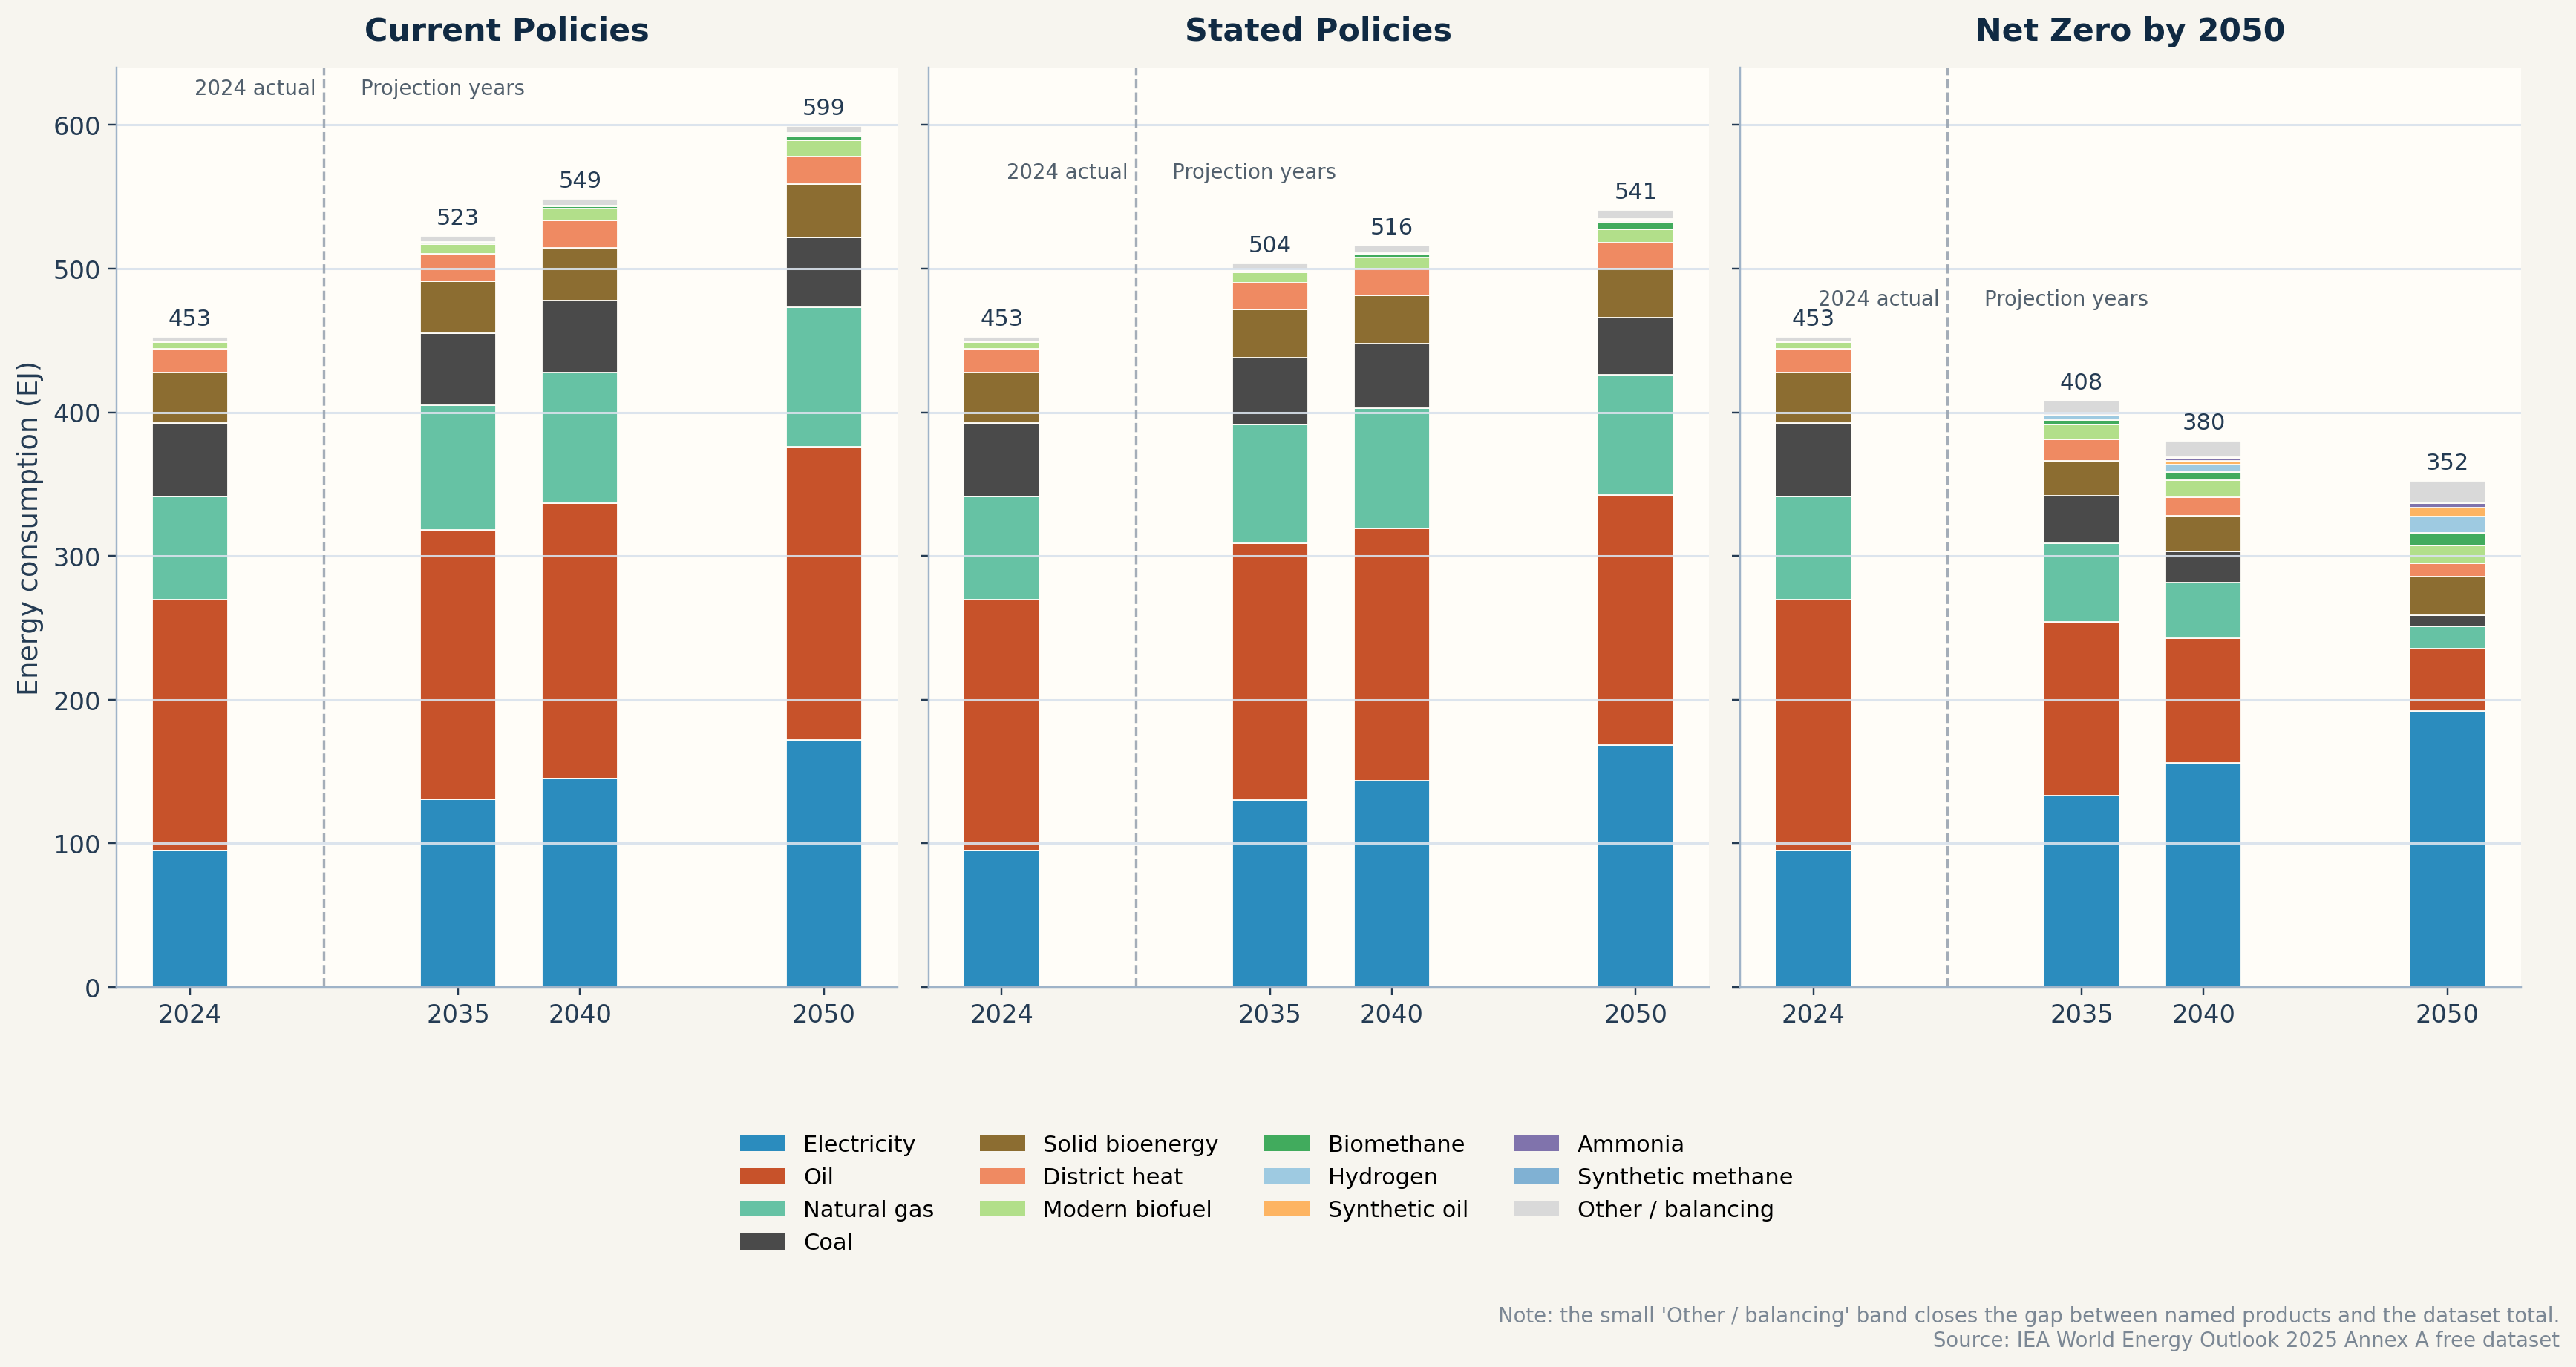
\includegraphics[width=\linewidth]{figures/world_energy_consumption_by_source_2050.png}
    \caption{World final energy consumption by source under the Current Policies, Stated Policies, and Net Zero Emissions by 2050 scenarios in the IEA World Energy Outlook 2025 free dataset.}
    \label{fig:world-energy-consumption-scenarios}
\end{figure}
 As shown in \Cref{fig:world-energy-consumption-scenarios}, global total final energy consumption rises from about 453~EJ in 2024 to roughly 599~EJ in 2050 in the Current Policies Scenario (CPS), where no strengthening of energy policies beyond those already in place is assumed. In the Stated Policies Scenario (STEPS), which incorporates a broader set of adopted and announced policy directions, demand still increases but more moderately, reaching about 541~EJ by 2050. By contrast, in the Net Zero Emissions by 2050 (NZE) Scenario, global final energy consumption falls to around 352~EJ by 2050, reflecting much stronger efficiency gains and a faster shift toward electrified end uses.

\begin{figure}[ht]
    \centering
    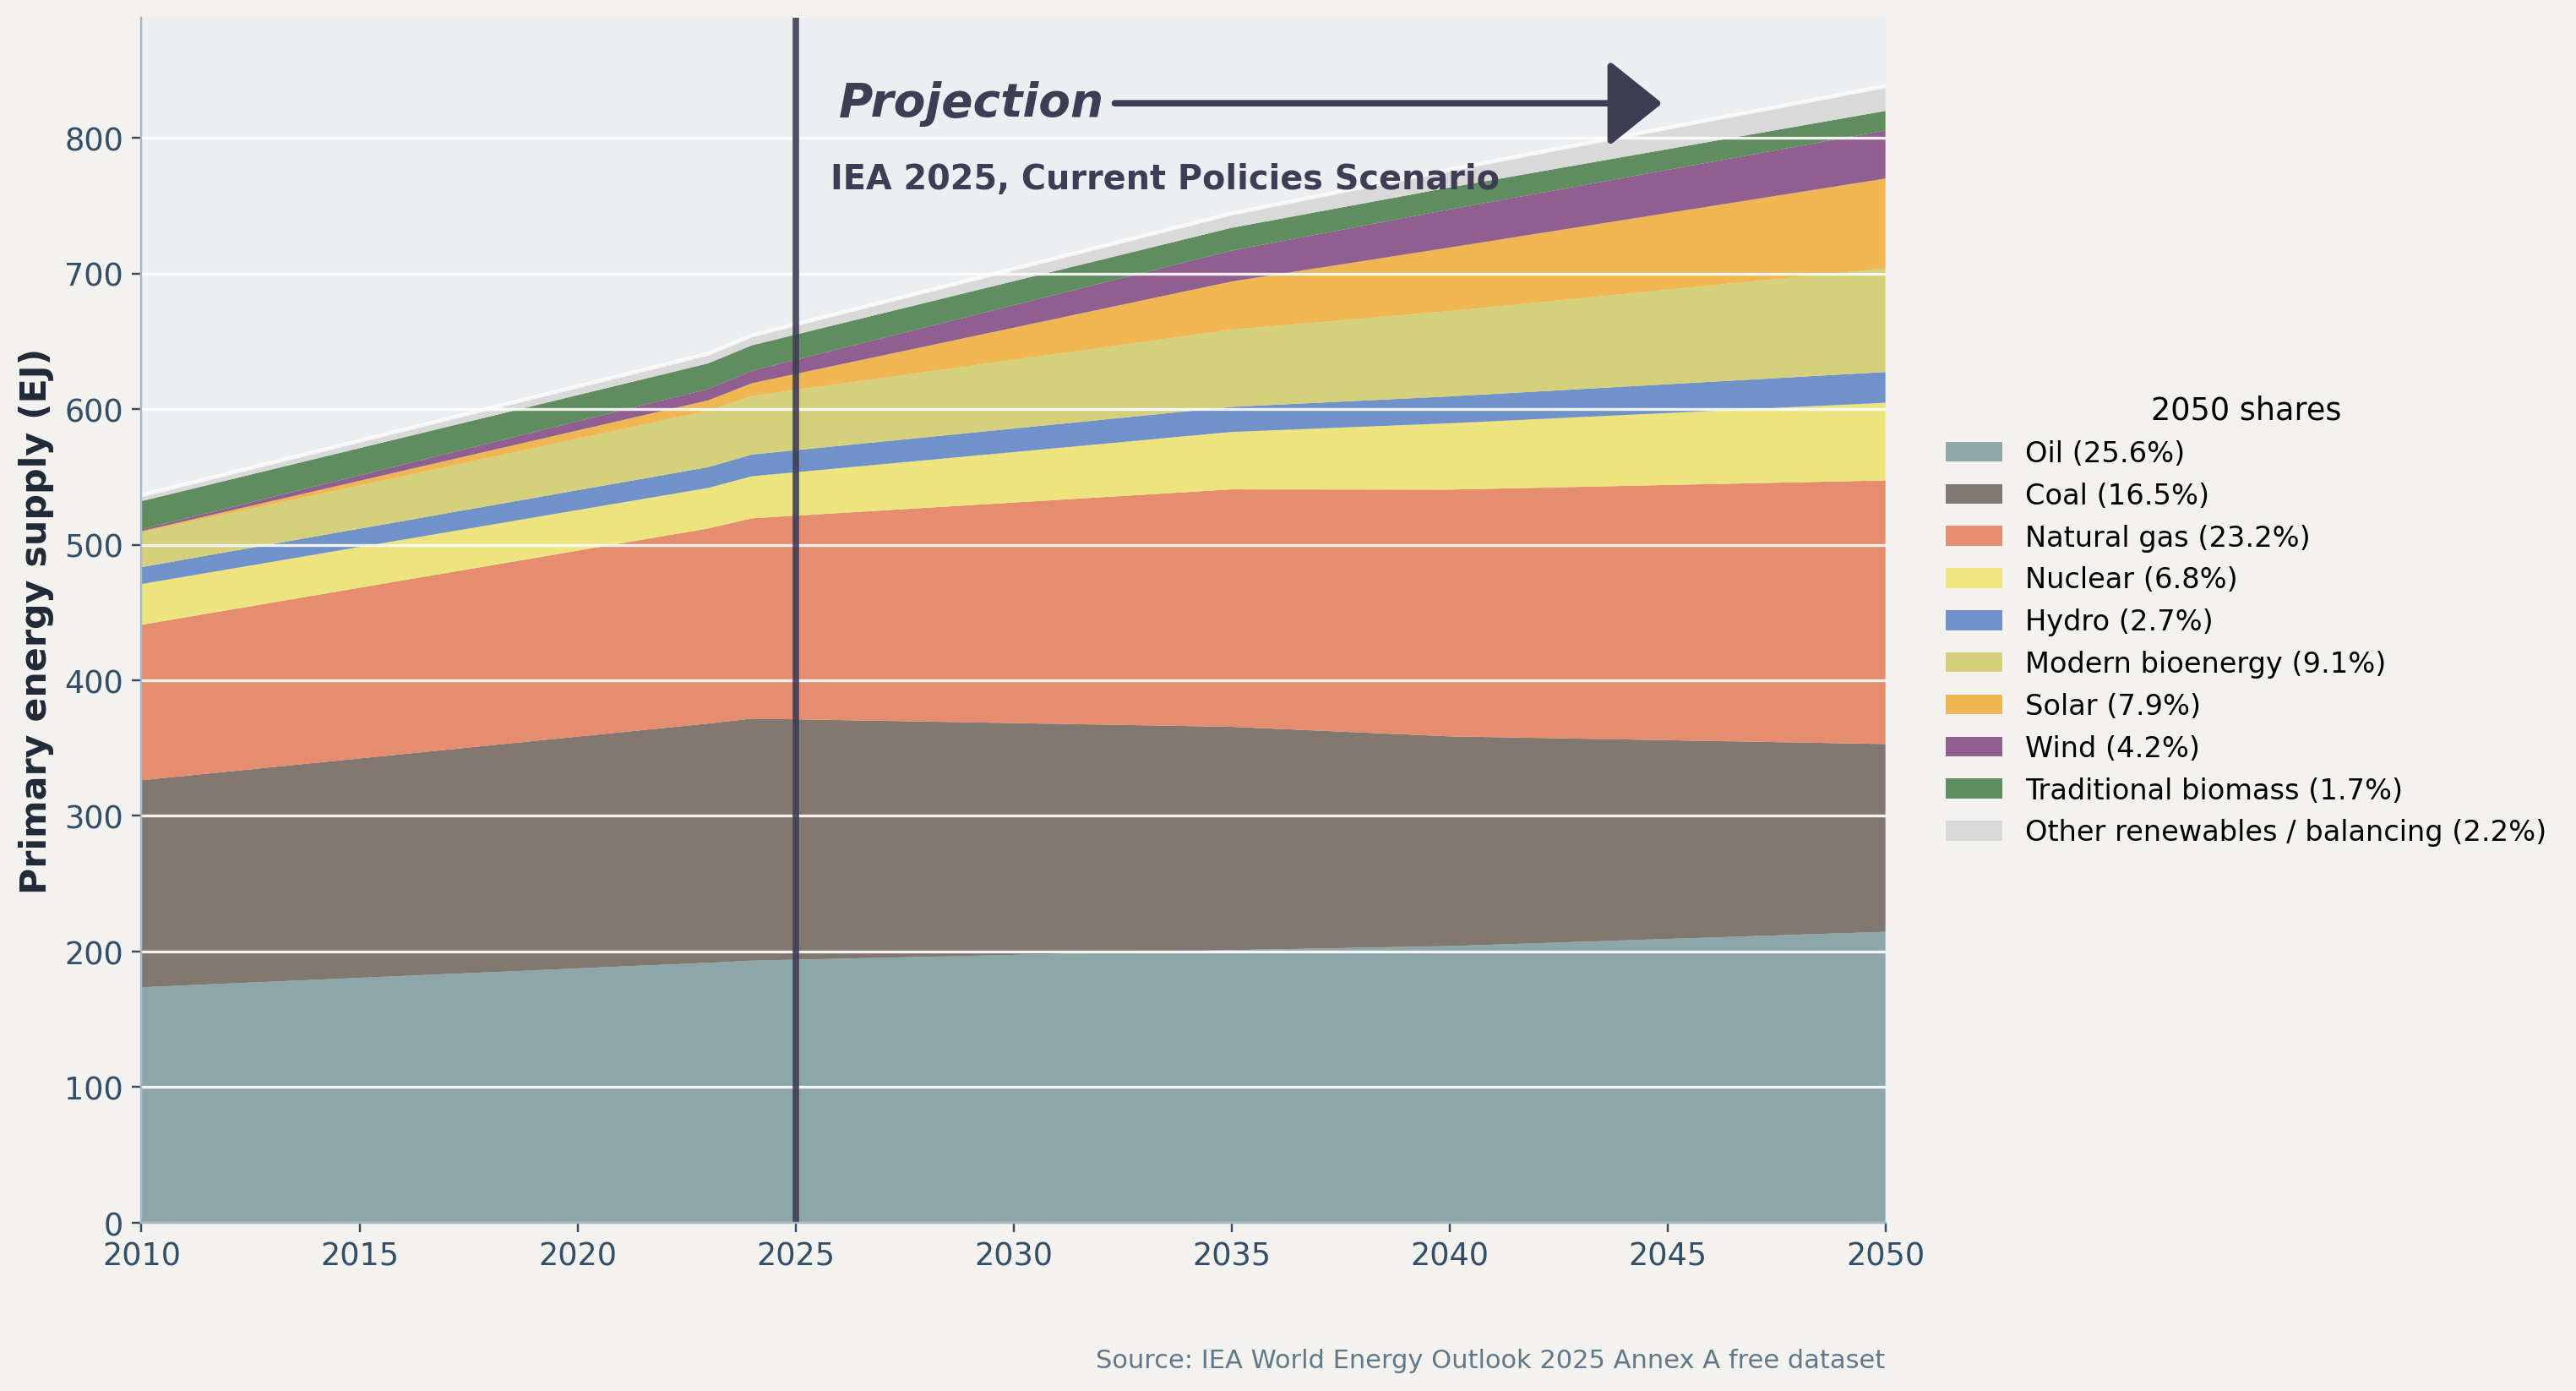
\includegraphics[width=\linewidth]{figures/world_energy_current_policies_shares_2050.png}
    \caption{World primary energy supply under the IEA World Energy Outlook 2025 Current Policies Scenario, with 2050 source shares shown in the legend.}
    \label{fig:world-current-policies-supply}
\end{figure}

\Cref{fig:world-current-policies-supply} complements this comparison by isolating the CPS pathway for world primary energy supply. Even in 2050, oil and natural gas remain the largest contributors, while solar, wind, nuclear, and modern bioenergy expand their shares substantially. This underlines why energy demand modelling is critical: future demand cannot be treated as a simple extrapolation of historical consumption, because it changes with assumptions about policy implementation, technology diffusion, fuel substitution, and energy efficiency. Scenario-based demand modelling is therefore essential for estimating future infrastructure needs, investment requirements, and emissions trajectories under different development pathways \cite{iea2025weo,iea2025gec}. 

\subsection{Technological Imperatives}
Inaccurate demand estimates can cause supply shortages or overcapacity, both of which drive price volatility and economic disruption. Geopolitically, detailed demand assessments also reveal import dependencies and exposure to external supply risks, informing diversification strategies and long-term energy-security policy.
\newline Beyond these considerations, there are fundamental technical reasons to map energy demand systematically, particularly in electricity. Power systems require real-time balancing: electricity must be consumed the instant it is generated \cite{WhyDoesElectricity}. If demand exceeds supply, system frequency drops and blackouts may follow; persistent overgeneration instead stresses system components \cite{ElectricalOvervoltageWhat}.

\subsubsection*{Grid frequency}
Frequency stability is thus a central operational constraint. In conventional systems dominated by large synchronous generators, the rotating masses of turbines and generators provide inertia. This does not eliminate imbalances but slows the rate at which frequency changes after a disturbance, buying time for control actions: after a sudden generation loss, inertia initially resists the frequency drop, after which primary frequency control, reserves, and other balancing services restore equilibrium. A lower-inertia system experiences a faster rate of change of frequency (RoCoF), leaving operators less time to respond and raising the risk of instability. Accurate demand modelling is therefore essential not only for energy accounting but for secure real-time operation, supporting reserve sizing, unit commitment, congestion management, and the anticipation of steep ramps and peak loads \cite{denholmInertiaPowerGrid2020}.

\subsubsection*{Infrastructure planning}
Demand mapping is equally critical for long-term infrastructure planning. Spatially resolved projections let policymakers and system operators anticipate urban growth, heating and transport electrification, and industrial development, informing timely investment in substations, transformers, transmission corridors, distribution reinforcements, and digital control infrastructure. Without sufficiently granular projections, network expansion can lag electrification, increasing congestion, curtailment, reliability risks, and total system cost \cite{entsoe_inertia_rocof_2020}.

\subsubsection*{Renewables}
The growing share of variable renewables such as wind and solar PV further raises the importance of detailed demand analysis. As noted in \Cref{sec:renewable_energy}, these resources are weather-dependent and only partially dispatchable, so their output need not coincide with peak demand. Many are also connected through power electronics rather than synchronous machines, so replacing thermal generation with inverter-based resources can reduce synchronous inertia, short-circuit strength, and the conventional frequency response naturally available, unless dedicated measures are introduced \cite{ElectricitySecurityMatters}. This again underscores the rising need for flexibility and coordination.

\subsection{Residential Energy Mix}\label{sec:residential_energy_mix}
A domestic (or residential) load is the energy a household uses to power all its appliances and devices, varying between households with their needs and consumption patterns.
\newline The residential sector is a significant source of energy-related GHG emissions, accounting for roughly 11\% of the global total once both direct fuel combustion and the indirect emissions from electricity and heat generation are included \cite{ritchieEmissionsBySector2020}. In 2023 it represented 26.2\% of EU final energy consumption \cite{EnergyConsumptionHouseholds}.
\newline Heating and cooling dominate household energy use in most countries. According to the IEA, the largest energy sources in Belgium's residential sector are natural gas and oil, at roughly 43\% and 27\% of residential final consumption respectively (\Cref{fig:BE_resi_consumption_mix}), with electricity (\textasciitilde20\%) and biofuels and waste (\textasciitilde9\%) making up most of the remainder \cite{IEA_ResidentialTFC_Belgium}. The sector is less well understood than commercial, industrial, agricultural, and transport demand, which benefit from more centralised ownership, stronger incentives and expertise in cutting consumption, and higher levels of regulation and documentation \cite{swan_modeling_2009}.
\begin{figure}[ht]
    \centering
    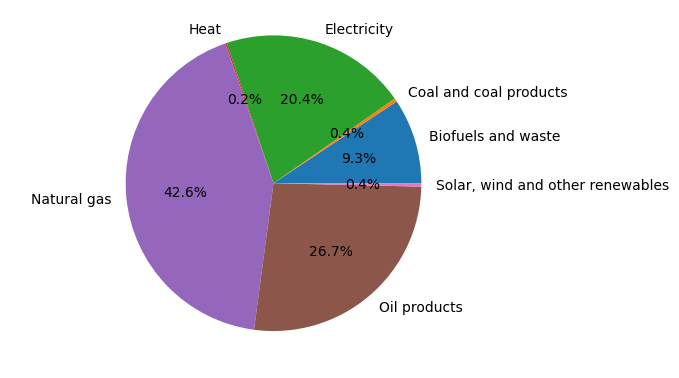
\includegraphics[width=0.8\linewidth]{figures/BE_resi_consumption.png}
    \caption{Belgian residential consumption mix in 2023; source: \href{https://www.iea.org/countries/belgium}{IEA}}
    \label{fig:BE_resi_consumption_mix}
\end{figure}
The residential sector consumes secondary energy: energy delivered ready for use to support occupants' living standards. Its main end-use groups are space heating and cooling (SH/SC), domestic hot water (DHW), and appliances and lighting. SH and SC offset thermal losses through the building envelope—conduction, radiation, and air infiltration/ventilation—to maintain a comfortable indoor temperature; DHW heats water for occupant and appliance use; and appliances and lighting power common devices (e.g.\ refrigerators, coffee makers) and provide adequate lighting. The relative weight of each group depends strongly on climate, building and system characteristics, appliance ownership, and occupant behaviour \cite{swan_modeling_2009}.

\subsubsection*{Electrifying the residential sector}
Many end uses in modern economies—lighting, information technology, household appliances, and air conditioning—are already electricity-based, but a large share of thermal demand is still met by directly combusting fuels: natural gas, heating oil, coal, and biomass remain widely used for space heating, DHW, and cooking. Electrifying these end uses is therefore a key mitigation pathway. Replacing fossil-fuel boilers with high-efficiency electric heat pumps can sharply reduce CO$_2$ emissions, especially as the electricity supply shifts toward low-carbon generation \cite{BelgiumCountriesRegions}, coupling end-use sectors to a progressively decarbonised power system.
\newline The transformation of the energy system should thus not be read as a trade-off between environmental and socio-economic objectives, but as a response to a single interconnected challenge. The same fossil-fuel combustion that drives environmental degradation also harms public health through air pollution, strains economies through climate-related damages, and undermines long-term societal stability. Decarbonising energy systems therefore advances environmental integrity, human well-being, and economic resilience together, since these dimensions are inherently interdependent.

\subsubsection*{New energy variables}
Historically, energy demand patterns exhibited relatively stable and predictable structures. Daily load curves largely reflected diurnal solar cycles\footnote{Diurnal solar cycles are the 24-hour patterns of change in sunlight, temperature, and atmospheric conditions driven by Earth's daily rotation. These cycles dictate the fluctuation between day and night, affecting energy input and causing daily temperature maximums in the afternoon and minimums at sunrise \cite{DiurnalCycle2025}.} and conventional work-week rhythms, with identifiable morning and evening peaks and reduced demand during nighttime and weekends. Under such conditions, forecasting approaches based primarily on historical time series and seasonal adjustments were often sufficient for operational planning.
\newline In contemporary energy systems, however, demand dynamics have become significantly more complex. Several structural developments contribute to this increased complexity:

\paragraph{Expansion of data centres.} 
Modern data centres require large amounts of continuous electricity, often operating as near-constant baseload consumers. Unlike residential loads, which fluctuate with occupancy patterns, data centre demand is relatively inelastic and geographically concentrated, placing sustained pressure on local grids.

\paragraph{Electrification of transport.} 
The rapid adoption of EVs introduces millions of distributed, mobile storage units into the electricity system. Charging behaviour is heterogeneous and time-dependent, often shifting demand from centralized workplace charging toward residential evening peaks. Without coordinated smart charging strategies, this can exacerbate peak loads and increase network congestion.

\paragraph{Climate variability.} 
Climate change introduces greater uncertainty into heating and cooling demand. Rising temperatures increase cooling loads, while more frequent and intense weather events reduce the reliability of historical data as a predictor of future energy consumption patterns. Traditional forecasting models calibrated on stationary climate assumptions may therefore become less accurate over time.

These developments fundamentally alter the temporal and spatial characteristics of energy demand. Consequently, accurate demand assessment can no longer rely solely on extrapolation of historical trends. Robust and physically grounded modelling frameworks are required to capture behavioural, technological, and climatic drivers of consumption. In this context, energy demand modelling emerges as a critical tool.


% \subsection{Residential Technologies}
% \label{sec:residentialTechnologies}
% % difference emitter vs conversion technologies
% % share of houses using PV, EV, heat pumps + boilers/gas in belgium

% \subsubsection*{Photovoltaics}
% %% 1-2 liner explanation on what PV is and how it works
% %% example of how it could be modelled, both simply and complex

% \subsubsection*{Electric vehicles}
% %% 1-2 liner explanation on what EV is and how it works
% %% example of how it could be modelled, both simply and complex

% \subsubsection*{Heat pumps}
% %% 1-2 liner explanation on what HP is and how it works: e.g.: 
% A heat pump (HP) uses mechanical work to pump heat from a low temperature to a high temperature. (the reverse of a heat pump is a refrigerant), using the vapor compression cycle.  The COP of a heat pump is a measure of its efficiency, calculated as the ratio of useful heat output (kW) to electrical power input (kW): $\text{COP}_\text{HP} = \frac{\dot{Q}_\text{H}}{\dot{W}_\text{in}}$ or $\text{COP}_\text{R} = \frac{\dot{Q}_\text{L}}{\dot{W}_\text{in}}$. However, this is an idealisation, referred to as the COP of Carnot, the ultimate efficiency that a heat pump can have. In reality, a pinch ($\Delta T)$ is necessary to drive the ``spontaneous'' heat transfer. Thus:
% \begin{align}
%     \text{COP}_\text{HP} &= \frac{\dot{Q}_\text{H}}{\dot{W}_\text{in}} = \frac{T_\text{H} + \Delta T}{T_\text{H} - T_\text{L} + 2\Delta T}\\
%     \text{COP}_\text{R} &= \frac{\dot{Q}_\text{L}}{\dot{W}_\text{in}} = \frac{T_\text{L} - \Delta T}{T_\text{H} - T_\text{L} + 2\Delta T}
% \end{align}
% %% example of how it could be modelled, both simply and complex, using HP implementation document (perhaps)?
% \paragraph{air-air HP}
% \paragraph{water-air HP}
% \paragraph{water-water HP}
% \paragraph{ground-source HP}

% \subsubsection*{Emitters}

\subsection{Residential Technologies}
\label{sec:residentialTechnologies}

Residential energy demand depends not only on the building envelope but on the technologies that convert energy carriers into useful services. These split usefully into \textit{conversion} technologies—which turn a carrier into heat, electricity, or mobility (gas boilers, heat pumps, PV systems, electric vehicles)—and \textit{emitter} technologies, which instead shape the conversion device's operating conditions. Radiators, underfloor heating, and fan coils, for instance, set the supply temperature a heating system must deliver and thus strongly affect heat-pump performance.

\subsubsection*{Belgian residential technology Stock}
Belgium's residential stock remains heavily fossil-based for space heating. The JRC reports roughly 2.8 million households using gas boilers against an installed heat-pump stock of about 209,000 units in 2022, when heat pumps made up only 11.8\% of combined heat-pump and boiler sales \cite{JRC2022HeatPumpBelgium}. Electrified technologies are nonetheless gaining ground: cumulative PV capacity reached 11.7\,GW in 2024, still dominated by sub-10\,kW residential systems \cite{vermang2024_pvps_belgium}. The same trend appears in transport, where households averaged 1.06 cars in 2024 \cite{StatbelHouseholds2025} amid a steadily hybridising and electrifying passenger fleet \cite{Statbel2025EV}. Such technologies are key boundary conditions for residential demand modelling, as they reshape both the annual energy balance and the timing of electricity demand.

\subsubsection*{Photovoltaics}

PV systems convert incident solar irradiance into direct-current electricity through the photovoltaic effect, after which an inverter converts the generated power to alternating current for household use or grid export. In residential applications, PV mainly acts as an on-site electricity-generation technology that reduces net grid import during sunny periods and can increase local self-consumption when combined with flexible demand, batteries, heat pumps or electric-vehicle charging.
\newline A simple PV model can represent generation as a linear function of plane-of-array irradiance and installed peak capacity:
\begin{equation}
    P_\text{PV}(t) = \eta_\text{PV} A_\text{PV} G_\text{POA}(t),
\end{equation}
where $\eta_\text{PV}$ is the module efficiency, $A_\text{PV}$ is the active module area and $G_\text{POA}$ is the plane-of-array irradiance. Equivalently, the system can be represented through a specific yield or capacity-factor profile multiplied by installed capacity. More detailed models add module temperature, inverter efficiency, orientation, tilt, shading, soiling and degradation effects \cite{duffie2013_solar_engineering,desoto2006_solar_model}. 
\newline For residential stock modelling, the appropriate level of detail depends on whether PV is used only as an annual energy contribution or whether the interaction with hourly household demand and self-consumption is analysed.

\subsubsection*{Electric vehicles}
An EV stores electrical energy in a battery and converts it into mechanical work through an electric drivetrain. For residential energy modelling, the vehicle itself is less important than its charging behaviour: arrival time, departure time, charger power, required trip energy, state of charge and user flexibility determine how mobility demand appears as household electricity demand.
\newline A simple EV model can assign a fixed daily charging energy to households with an EV and distribute it over an evening charging window:
\begin{equation}
    E_\text{EV,day} = e_\text{km} d_\text{day},
\end{equation}
where $e_\text{km}$ is the specific electricity consumption per kilometre and $d_\text{day}$ is the daily driven distance. A more detailed model could sample trips, arrival times, plug-in probability, charging power, battery capacity and state-of-charge (SoC) constraints, so that the charging load becomes an event-based process rather than a fixed profile \cite{richardson2013_ev_demand,muratori2018_ev_charging}. This distinction matters because uncontrolled EV charging can amplify evening peaks, while delayed or smart charging can shift demand toward periods of PV production or lower system load.

\subsubsection*{Heat pumps}
A heat pump (HP) uses mechanical or electrical work to move heat from a lower-temperature \textit{source} to a higher-temperature \textit{sink}. In heating mode, useful heat is delivered to the dwelling; in cooling mode, heat is removed from the conditioned space. The ideal heat-pump coefficient of performance is bounded by the Carnot limit:
\begin{equation}
    \text{COP}_{\text{HP,Carnot}}
    =
    \frac{T_\text{H}}{T_\text{H}-T_\text{L}},
\end{equation}
where $T_\text{H}$ and $T_\text{L}$ are absolute sink and source temperatures. For refrigeration or cooling, the corresponding ideal coefficient is:
\begin{equation}
    \text{COP}_{\text{R,Carnot}}
    =
    \frac{T_\text{L}}{T_\text{H}-T_\text{L}}.
\end{equation}
In practice, finite temperature differences are required in the evaporator and condenser to drive heat transfer. If a simplified temperature approach $\Delta T$ is introduced, the effective evaporating temperature is lower than the source temperature and the condensing temperature is higher than the sink temperature:
\begin{align}
    \text{COP}_\text{HP}
    &\approx
    \frac{T_\text{H} + \Delta T}
    {T_\text{H} - T_\text{L} + 2\Delta T}, \\
    \text{COP}_\text{R}
    &\approx
    \frac{T_\text{L} - \Delta T}
    {T_\text{H} - T_\text{L} + 2\Delta T}.
\end{align}
These expressions remain idealised, but they show the central physical dependency: heat pumps perform better when the temperature lift between source and sink is small~\cite{moran2018_thermodynamics,staffell2012_review_heat_pumps}.
\newline A simple heat-pump model can use a fixed seasonal performance factor (SPF) or constant COP:
\begin{equation}
    P_\text{el,HP}(t) =
    \frac{\dot{Q}_\text{useful}(t)}{\text{COP}}.
\end{equation}
This is sufficient for coarse annual energy balances, but it hides the dependence on outdoor temperature and supply temperature. More detailed models calculate COP as a function of source temperature, sink temperature, part-load operation, defrost losses\footnote{Defrost is the process where an air-source heat pump removes ice/frost from its outdoor coil. The frost comes from the moisture of the cold and humid air that freezes on the coil. That frost blocks airflow and reduces heat transfer, so the heat pump becomes less efficient.} and emitter type. This is particularly relevant in Belgian dwellings, where existing buildings often require higher supply temperatures than new low-temperature heating systems.

\paragraph{Air-air heat pumps.}
An air-air heat pump extracts heat from outdoor air and supplies heat directly to indoor air. It usually has relatively low distribution losses and can also provide active cooling, but it does not directly feed a hydronic radiator or DHW system. In residential models, it can be represented as an electricity-driven space-conditioning unit with outdoor-air temperature as the source and indoor air as the sink.

\paragraph{Air-water heat pumps.}
An air-water heat pump extracts heat from outdoor air and delivers heat to a water-based distribution system. This is one of the most relevant heat-pump types for residential space heating because it can replace or supplement boiler-based hydronic systems. Its performance is strongly affected by the required water supply temperature: underfloor heating and low-temperature radiators generally allow higher COPs than standard or high-temperature radiators.

\paragraph{Water-water heat pumps.}
A water-water heat pump uses water as the heat source and water as the heat sink. The source can be groundwater, surface water or another water loop. Since water-source temperatures are often more stable than outdoor air temperatures, water-water systems can achieve high and stable COPs. However, they are more site-specific and depend on hydraulic, environmental and regulatory constraints.

\paragraph{Ground-source heat pumps.}
A ground-source heat pump extracts heat from the ground through horizontal loops, vertical boreholes or brine circuits. The ground source is less variable than outdoor air, which reduces seasonal COP variation and avoids most defrost-related losses. The drawback is the higher installation complexity and cost, especially in dense residential areas or existing buildings.

\subsubsection*{Emitters}
Emitter systems transfer useful heat from the conversion technology to the indoor zone; common residential types are standard radiators, low-temperature radiators, underfloor heating, and fan coils. Their relevance to energy modelling lies in their required supply temperature. A gas boiler can deliver high supply temperatures with little efficiency penalty, whereas a heat pump loses efficiency as the sink temperature rises. The same heat pump can therefore draw different amounts of electricity depending on whether it serves underfloor heating, low-temperature radiators, or older high-temperature radiators.
\newline Simplified stock models can represent emitters through a fixed design supply temperature per dwelling class. A more detailed option is weather-compensated control, where the flow temperature tracks outdoor temperature rather than staying at the design maximum all season \cite{home_energy_model_heat_pumps_2026}:
\begin{equation}
    T_\text{supply}(t)
    =
    T_\text{low}
    +
    f(T_\text{out}(t))
    \left(
    T_\text{high} - T_\text{low}
    \right).
\end{equation}
This captures the link between building heat demand, outdoor conditions, emitter type, and heat-pump COP without a full hydraulic simulation. In technology scenarios, emitter assumptions thus decide whether heat-pump electrification is modelled as a low-temperature, high-COP pathway or a higher-temperature retrofit with lower seasonal performance.


\pagebreak
\section{Energy Demand Modelling}

Energy demand modelling can be defined as the quantitative determination of present and future energy consumption patterns through mathematical and computational models. These models are used to represent the structural drivers of demand and to project both long-term trends and short-term fluctuations. In doing so, they support system planning, sustainability assessment, and infrastructure optimization \cite{verwiebe_modeling_2021}. Depending on the modelling paradigm\footnote{A model's paradigm refers to the fundamental approach used to construct it.} adopted, demand models may range from high-level econometric representations to detailed, \hyperref[sec:bottom_up]{bottom-up} simulations of individual buildings and technologies. 
\newline \Cref{fig:modelling_framework} shows a \hyperref[sec:bottomUpModelling]{bottom-up modelling} framework adopted by Cruz et al.'s modelling paradigm.

\begin{figure}[ht]
    \centering
    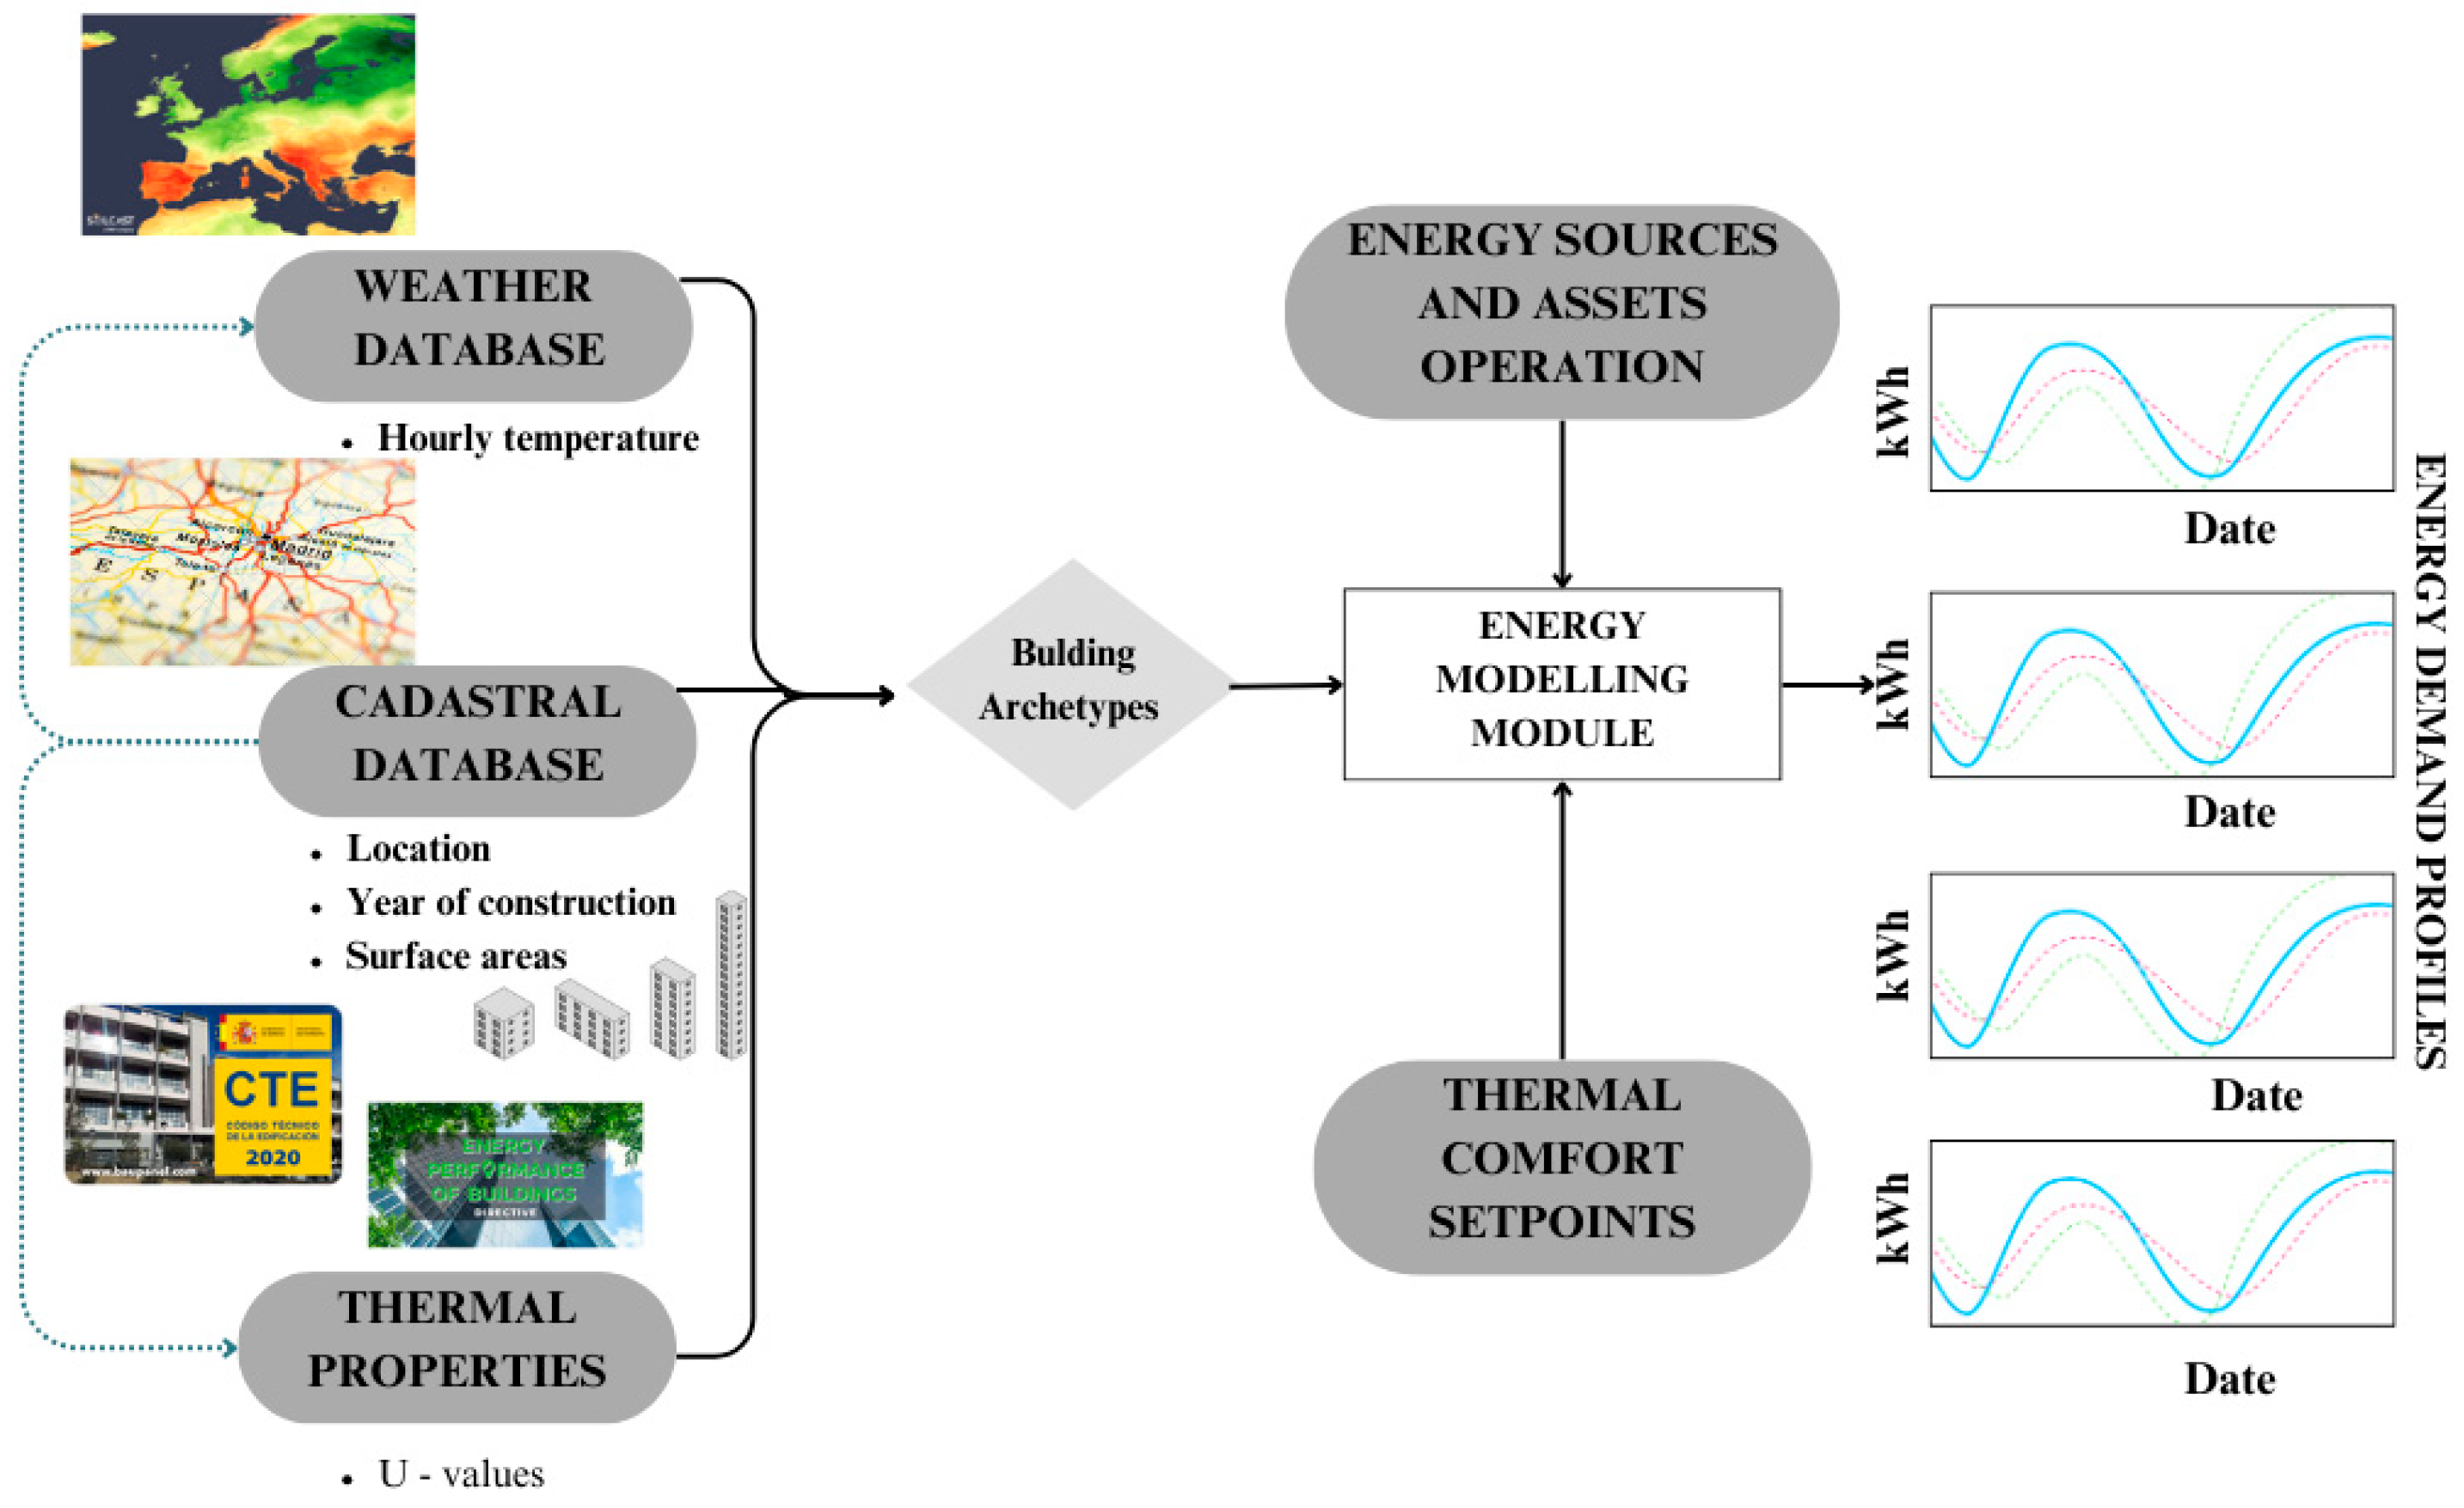
\includegraphics[width=0.8\linewidth]{figures/modelling_framework.png}
    \caption{Energy consumption modelling framework; source: Cruz et al.\cite{cruzDevelopmentEnergyDemand2025}}
    \label{fig:modelling_framework}
\end{figure}

Energy demand models are applied across multiple spatial and temporal scales. At the macro scale, they are commonly used to estimate regional, national, or supranational energy requirements and to inform long-term capacity expansion planning. At the micro scale, models can quantify the change in energy consumption of a specific dwelling\footnote{A dwelling is a home—see \Cref{sec:residential_eED_modelling} for a more detailed explanation.} due to technological upgrades, retrofits, or behavioural shifts. Such analyses are particularly relevant in the residential sector, where improvements in insulation, heating systems, glazing, or control strategies can significantly alter consumption profiles. By estimating both baseline demand and potential savings, these models provide quantitative support for policy decisions related to building codes, retrofit incentives\footnote{Retrofit incentives are financial or regulatory measures designed to encourage the upgrade of existing buildings or systems to improve their performance, typically in terms of energy efficiency or emissions reduction.}, electrification strategies, and long-term infrastructure investment \cite{swan_modeling_2009}.

% Models may be used for a variety of reasons, the most common being the determination of regional or national energy supply (macro-scale) requirements and the change in energy consumption of a particular dwelling\footnote{A dwelling is a home — somewhere to live.} due to an upgrade or addition of technology (micro-scale). Modelling of this nature is useful as it can guide decisions of policy regarding the residential stock, both old and new. By quantifying the consumption and predicting the impact or savings due to retrofits and new materials and technology, decisions can be made to support energy supply, retrofit and technology incentives, new building code, or even demolition and re-construction \cite{swan_modeling_2009}.

\subsection{Modelling Challenges}
A persistent challenge in energy modelling is the representation of occupant behaviour—especially within \hyperref[sec:residential_eED_modelling]{residential energy modelling}. Traditional engineering models often assume deterministic usage patterns or standardized occupancy schedules. However, empirical evidence shows that occupant behaviour is dynamic, heterogeneous, and influenced by a complex interplay of internal and external factors. These include socio-demographic characteristics, cultural norms, economic incentives, comfort preferences, building design, and real-time environmental conditions \cite{delzendehImpactOccupantsBehaviours2017}. The stochastic and adaptive nature of occupant interactions with heating, cooling, ventilation, and appliance systems introduces substantial uncertainty into building energy predictions. Addressing this complexity requires a multidisciplinary approach that integrates perspectives from sociology, psychology, economics, and behavioural sciences alongside engineering and design. 
\newline Thus, understanding occupants’ motivations, decision-making processes, and interaction patterns with building systems is essential for improving the predictive accuracy of demand models. Incorporating behavioural variability into modelling frameworks enhances their \hyperref[sec:realism]{realism} and strengthens their relevance for policy design, demand-side management, and long-term decarbonization planning \cite{delzendehImpactOccupantsBehaviours2017}.


\subsection{Stock Models}
% what is a stock model, how does it fit in the energy demand model paradigm?
Although the two fields overlap significantly, energy \textit{stock} modelling and energy \textit{demand} modelling are not the same. While the former provides the structural parameters of buildings, the latter simulates the dynamic energy flows. Residential stock modelling describes the ``shell'' (what exists), while residential energy demand modelling describes the ``energy flow'' (what happens inside) \cite{mahmoudOpportunitiesLimitationsBuilding2020}.

\subsubsection*{Building stock models}
Building stock energy refers to the aggregate energy consumption of all buildings in a given area. In the EU the building sector is a major share of final energy use and GHG emissions, with roughly 75\% of buildings classified as poor energy performers \cite{nageliBestPracticeReporting2022}. Because buildings are long-lived assets, decarbonising the stock is a structural challenge, and EU policy accordingly emphasises large-scale renovation and efficiency strategies. Building stock models are the central tool here: they let policymakers simulate renovation pathways, assess cost-optimal retrofits, estimate emission reductions, and track progress toward 2050 climate neutrality \cite{EUBuildingStock}, quantifying through scenario analysis the stock-wide impact of insulation upgrades, heating electrification, or district-heating expansion.
\newline Such models represent an entire building population within a defined area (city, region, or country) as a structured ensemble of archetypes, rather than a single building. Each archetype is characterised by parameters such as building type, construction period and typology, heating, cooling and DHW systems, and envelope properties such as U-values\footnote{The U-value measures how effectively a building element resists heat transfer, in W/m²K, across all its layers \cite{yuUValuesBuildingEnvelopes2024}.}. Aggregating these archetypes and scaling them to statistical data yields estimates of total energy demand, emissions, and renovation impacts at system scale \cite{hongTenQuestionsBuilding2025}. Building stock modelling is closely related to residential energy demand modelling but operates at a more aggregated, policy-oriented level; this review therefore concentrates on demand-modelling methodologies rather than large-scale stock transition modelling.


\subsubsection*{Residential stock models}
Residential stock modelling focuses on representing the structural composition and long-term evolution of the housing sector. Its primary objective is to characterize the building fleet at an aggregated level. Such models aim to provide a structured description of the physical and technical attributes of dwellings across a defined region \cite{hongTenQuestionsBuilding2025}.
\newline Although the present literature review focuses on residential buildings—specifically dwellings—it does not primarily address residential stock modelling in the structural or policy-oriented sense described above. Instead, the emphasis lies on modelling residential energy consumption: that is, the dynamic and quantitative simulation of energy use within dwellings.


\subsubsection*{Comparing stock and demand}
Table \ref{tab:modelling_framework_comparison} compares the two aforementioned modelling frameworks. 

\begin{table}[ht]
\centering
\caption{Comparison between residential stock modelling and residential energy cemand modelling}
\label{tab:modelling_framework_comparison}
\begin{tabular}{p{3cm} p{5cm} p{5cm}}
\toprule
\textbf{Aspect} & \textbf{Stock Modelling} & \textbf{Energy Demand Modelling} \\
\midrule
Focus & What buildings exist? & energy consumption \\
Nature & Structural, static & Dynamic, temporal \\
Time resolution & Usually none or annual & Hourly or sub-hourly \\
Core variable & U-values, system type & kWh, load profiles \\
Uncertainty type & Structural uncertainty & Behavioural + climate + system \\
\bottomrule
\end{tabular}
\end{table}
From a modelling pipeline perspective; the relation between the two frameworks could possibly look like this:
$$ \text{Building Stock Model  →  Parameterisation  →  Energy Demand Model} $$


\subsection{Residential Energy Demand Modelling}\label{sec:residential_eED_modelling}
Residential energy demand modelling quantifies household energy consumption over time. While it often draws on ``stock data'' as input, its main concern is the physics of energy use and human behaviour within a given \textit{dwelling} \cite{zhangModelingManagingResidential2025}. It answers questions such as: what is a household's hourly electricity demand, the annual space-heating demand of detached houses, the load profile of a community, or the change in demand under electrification or climate warming?

A dwelling—detached or semi-detached house, terraced house, flat, studio, and so on—is defined by having its own living spaces and facilities (sleeping, cooking, sanitation) separate from other units. Summing each dwelling's consumption across an area (city or country) gives the regional or national residential energy consumption that is the focus of this thesis.

Such models rely on input data to calculate or simulate consumption. The level of detail of that data varies dramatically, leading to different modelling techniques that exploit the available information, each with distinct strengths, weaknesses, capability, and applicability \cite{swan_modeling_2009}.


\subsection{Modelling Approaches}\label{sec:modelling_approaches}
Techniques used to model residential energy consumption are generally classified into two principal categories: top-down and bottom-up approaches. The distinction refers to the hierarchical level at which modelling inputs are introduced relative to the housing sector as a whole \cite{swan_modeling_2009}.

\subsubsection*{Overview of the top-down approach}
Top-down models begin at the aggregated level. They use macro-scale data—such as total residential energy consumption, gross domestic product\footnote{GDP is the total monetary value of all final goods and services produced within a country's borders during a specified period and is the most common measure of a nation's economic size and health.} (GDP), energy prices, demographic indicators, or climatic variables—to statistically attribute energy use to sector-wide characteristics. These models are typically econometric or regression-based and are well suited for national-level forecasting and policy analysis. However, they offer limited resolution regarding individual building characteristics or behavioural dynamics. 

\subsubsection*{Overview of the bottom-up approach}\label{sec:bottom_up}
Bottom-up models start at the micro scale. They simulate the energy consumption of individual dwellings or representative building archetypes based on physical properties, system specifications, occupancy patterns, and usage behaviour. The results are then aggregated to represent regional or national demand. Bottom-up approaches provide higher granularity\footnote{Granularity refers to the detail—both spatial and temporal—of the data/model.} and are particularly useful for evaluating retrofit strategies, electrification scenarios, and technology adoption pathways, because unlike the top-down approach, the bottom-up approach does have the ability to explicitly address the effect of occupant behaviour—which is a very important factor to consider when modelling energy consumption.

\subsubsection*{Top-down vs Bottom-up}
% Show table with pros and cons per modelling approach, also explain how they differ in realism and add a table that compares the two
Table \ref{tab:model_comparison} illustrates a comparative summary of the top-down and bottom-up approaches. The table summarizes their main characteristics, advantages, limitations, and relative level of \hyperref[sec:realism]{realism}.

\begin{table}[ht]
\centering
\footnotesize
\setlength{\tabcolsep}{4pt}
\renewcommand{\arraystretch}{1.2}
\caption{Comparison of top-down and bottom-up residential energy demand modelling approaches (adapted from Swan and Ugursal \cite{swan_modeling_2009}).}
\label{tab:model_comparison}
\begin{tabular}{>{\raggedright\arraybackslash}p{0.12\linewidth}
                >{\raggedright\arraybackslash}p{0.26\linewidth}
                >{\raggedright\arraybackslash}p{0.24\linewidth}
                >{\raggedright\arraybackslash}p{0.26\linewidth}}
\hline
\textbf{Approach} & \textbf{Main features} & \textbf{Advantages} & \textbf{Limitations / realism} \\
\hline
\textbf{Top-down} &
Uses aggregated sector-level energy data with macroeconomic, demographic, and climatic indicators; based on historical correlations and econometric models. &
- Suitable for long-term national or regional projections \newline
- Low data requirements \newline
- Computationally efficient &
- Limited technological granularity \newline
- Minimal behavioural representation \newline
- Lower physical realism \\
\hline
\textbf{Bottom-up} &
Estimates demand at the level of individual dwellings or archetypes, then aggregates to regional/national scale. Includes: \newline
(i) statistical methods \newline
(ii) engineering methods &
- Captures end-use detail \newline
- Can incorporate occupant behaviour \newline
- Suits retrofit and technology-impact analysis \newline
- Higher spatial and temporal resolution &
- Data intensive \newline
- Higher computational demand \newline
- Behaviour often simplified unless explicitly modelled \newline
- Requires calibration to reduce performance gap \newline
- Higher realism (physical + behavioural potential) \\
\hline
\end{tabular}
\end{table}

In terms of realism, top-down models provide the lowest structural fidelity because they rely on aggregate historical relationships rather than explicit physical representation. Bottom-up statistical models improve realism by capturing end-use diversity and behavioural correlations derived from empirical data. Bottom-up engineering models offer the highest level of physical realism, as they explicitly simulate thermodynamic processes and building-system interactions. However, their overall realism remains constrained if occupant behaviour is not represented stochastically or dynamically.
\newline Consequently, the choice of modelling approach depends on the research objective, data availability, and required resolution.


\subsection{Realism}\label{sec:realism}
In the context of energy demand modelling, realism refers to the extent to which a model accurately represents the physical, technical, and behavioural processes that determine actual energy consumption. A realistic model should not only reproduce aggregated annual consumption, but also capture temporal variability, system interactions, and user-driven dynamics that occur in practice.

\subsubsection*{Influential factors}
The energy consumption of buildings is influenced by a wide range of interacting factors, as is shown in \Cref{fig:influencing_factors}. These include the thermodynamic \& physical properties of buildings envelope, construction quality and detailing, climatic conditions, the performance and maintenance of HVAC systems, and—critically—the behaviour and activities of occupants \cite{delzendehImpactOccupantsBehaviours2017}, which is highlighted in \Cref{fig:influencing_factors} to emphasise its importance. 
\newline During the design phase, building energy simulation tools are typically employed to predict future consumption based on architectural plans, material specifications, and standardized occupancy assumptions. However, numerous empirical studies have documented a significant discrepancy between predicted and measured energy consumption in operational buildings \cite{delzendehImpactOccupantsBehaviours2017}. This discrepancy is commonly referred to as the performance gap.

\begin{figure}[ht]
    \centering
    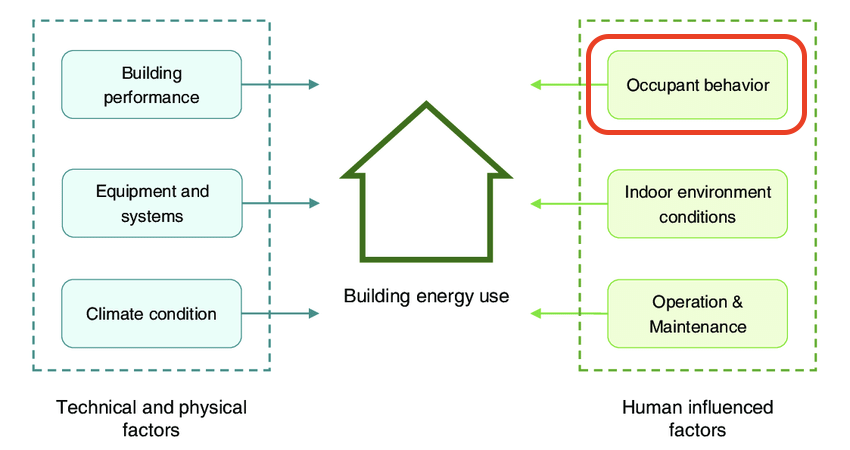
\includegraphics[width=0.8\linewidth]{figures/Six-influencing-factors-on-building-energy-use.png}
    \caption{Illustration of the six main influencing factors on a building's energy use; source: \href{https://www.researchgate.net/publication/337160052_China_Building_Energy_Use_2018}{China Building Energy Use 2018}}
    \label{fig:influencing_factors}
\end{figure}


\subsubsection*{Performance gap}
The performance gap arises from multiple sources. First, deviations between design intent and as-built construction—such as material substitutions, installation defects, or commissioning issues—can degrade performance. Second, operational conditions may differ from design assumptions. Most importantly, occupant behaviour is frequently simplified or treated deterministically in simulation tools. In reality, occupants exhibit heterogeneous, adaptive, and sometimes unpredictable behaviour patterns.

\subsubsection*{Occupant behaviour}
Research by Martinaitis and Zavadskas \cite{martinaitisImportanceOccupancyInformation2015} demonstrated that buildings often underperform relative to simulation results even when physical modelling is highly detailed, highlighting the decisive role of human behaviour. Similarly, Schakib-Ekbatan et al. \cite{schakib_ekbatanDoesOccupantBehavior2015} identified occupant behaviour as one of the most overlooked parameters in the entire chain of building design, construction, operation, and maintenance.
\newline Occupants influence energy use through variety of ways as displayed in \Cref{fig:behaviour_factors}. These behaviours are shaped by comfort preferences, socio-economic factors, cultural norms, and real-time environmental conditions. Because such behaviour is inherently dynamic with \hyperref[sec:stochastic_hetero]{stochasticity \& heterogeneity} at its core, deterministic schedules embedded in traditional simulation models often fail to capture realistic variability. As a result, improving the realism of building energy models increasingly requires explicit representation of occupant behaviour.

\begin{figure}[p]
    \centering
    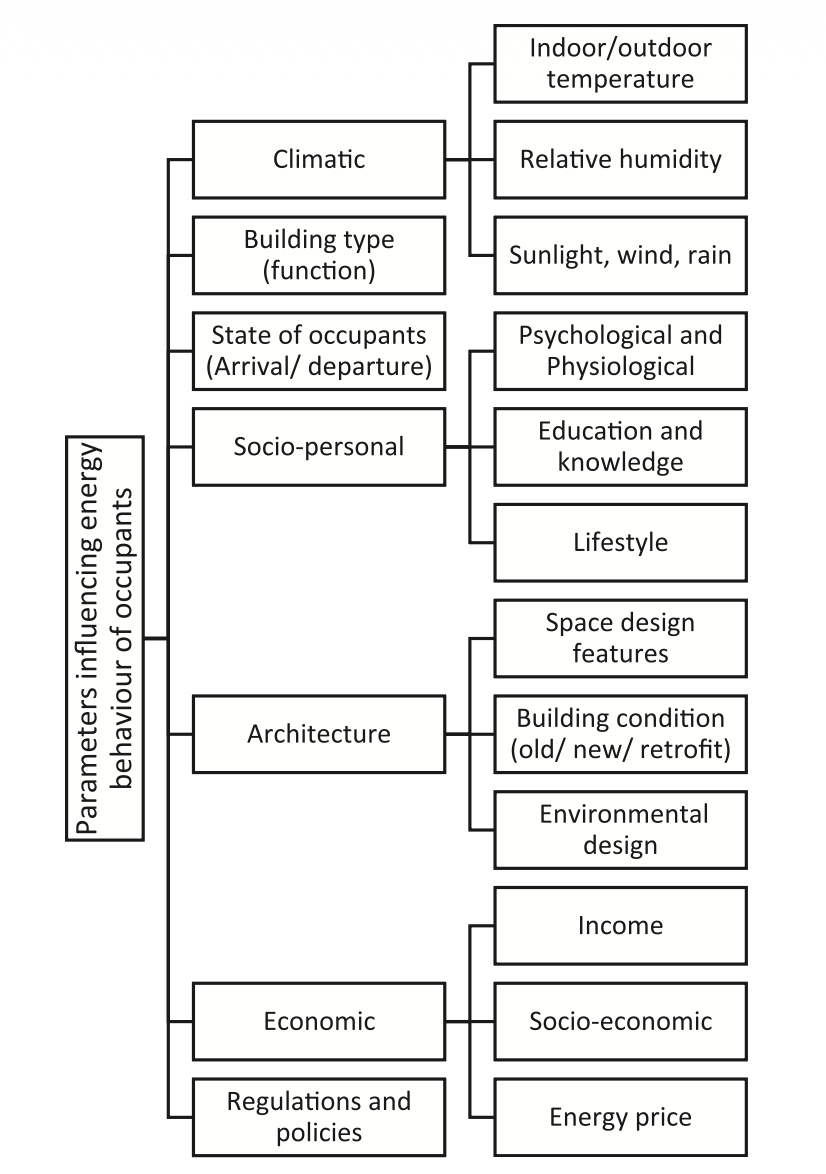
\includegraphics[width=0.8\linewidth]{figures/Behaviour_factors.png}
    \caption{Factors and sub-factors influencing energy behaviour of occupants \cite{delzendehImpactOccupantsBehaviours2017}.}
    \label{fig:behaviour_factors}
\end{figure}


\subsection{Uncertainty}
%%% what is uncertainty, how does it influence the models, what does the literature show, ...
The term ``uncertainty'' can be defined as the state of having limited knowledge about a system, making it difficult to predict future outcomes or describe current states accurately. A model which effectively captures different uncertainty sources has a higher degree of realism \cite{hongTenQuestionsBuilding2025,Smith2014}.

\subsubsection*{Sources of uncertainty}
One way to classify uncertainty sources is by distinguishing whether uncertainty is inherent to the system, due to lack of knowledge, or due to imperfect data \cite{Smith2014,Saltelli2008}.

\paragraph{Aleatoric uncertainty.}
This refers to the physical randomness of the system and is intrinsic — even with perfect knowledge, it does not disappear \cite{Smith2014}. In residential energy demand modelling, this is primarily associated with stochastic occupancy patterns and behavioural variability \cite{hongTenQuestionsBuilding2025}. This uncertainty is statistical in nature and must be modelled probabilistically.

\paragraph{Epistemic uncertainty.}
This arises from imperfect knowledge of the system or its parameters \cite{Smith2014}. In building energy models, this includes uncertainty in $U$-values, heat pump COP curves, thermal mass assumptions, and simplifications in model structure \cite{hongTenQuestionsBuilding2025,Hensen2011}. Unlike aleatoric uncertainty, epistemic uncertainty is reducible through improved data, calibration, and model refinement.

\paragraph{Data uncertainty.}
This refers to uncertainty introduced by imperfect, incomplete, or reconstructed data \cite{ASHRAE14}. Examples include missing weather data, smart meter gaps, temporal aggregation issues, and sensor noise. Such uncertainties propagate through the modelling pipeline and must be addressed prior to simulation.

To summarise, aleatoric uncertainty reflects inherent stochastic variability in occupant behaviour, epistemic uncertainty arises from incomplete knowledge of model parameters and structure, and data uncertainty originates from measurement errors and preprocessing steps, each requiring distinct modelling and validation strategies \cite{hongTenQuestionsBuilding2025,Smith2014}.


\subsection{Climate Uncertainty}
Climate conditions are a primary driver of residential energy demand, especially for space heating and cooling, which makes climate uncertainty a critical factor in energy modelling \cite{IPCC2021,DeWilde2014}. It arises from several sources: natural climate variability, structural differences between climate models, and uncertainty in future emissions scenarios \cite{IPCC2010}. In practice, this uncertainty enters through meteorological inputs such as outdoor temperature, solar irradiance, and wind speed. Temperature usually dominates thermal demand and is often approximated by aggregated indicators such as heating and cooling degree days (HDD/CDD) \cite{Clarke2001}. These are convenient but neglect temporal dynamics and non-linear system responses, which can bias demand estimates under changing climates \cite{DeWilde2014}.

A key distinction separates short-term variability, which drives demand fluctuations and peak loads, from long-term climate change, which shapes annual consumption and system sizing \cite{IPCC2021}. Representative weather datasets capture average conditions but miss extremes and inter-annual variability \cite{Wilcox2008}, so the literature increasingly favours multi-year datasets, stochastic weather generators, and climate-model ensembles to span a broader range of conditions \cite{Semenov2010,Saltelli2008}.
Integrating time-resolved weather variables directly into building energy models represents climate effects more consistently than aggregated indicators, which matters for non-linear processes such as thermal inertia, solar gains, and temperature-dependent system performance \cite{Clarke2001}. Explicitly accounting for climate uncertainty is therefore essential for robust, unbiased demand predictions under present and future climates \cite{DeWilde2014,IPCC2021}.


\subsection{Stochasticity \& Heterogeneity}\label{sec:stochastic_hetero}
In residential energy modelling, it is essential to distinguish between \textit{heterogeneity} and \textit{stochasticity}, as both concepts address different dimensions of aleatoric and epistemic uncertainty that drives a model's realism. 

Heterogeneity refers to systematic differences between households, whereas stochasticity refers to the time-varying and partly random behaviour within a given household. This distinction matters because empirical studies show that residential demand is neither well represented by a single “average household” nor by a deterministic repetition of the same daily routine. Instead, both the level of annual consumption and the timing of short-term demand events vary substantially across and within homes \cite{beis_ofgem_lv_network_capacity_2022}.

\subsubsection*{Heterogeneity}
Heterogeneity is clearest in the distribution of annual household demand: households do not consume uniformly. The differences stem from socio-demographic, technical, and environmental factors—occupant numbers, work and school schedules, lifestyle (e.g.\ cooking versus dining out), appliance ownership, and thermal-comfort expectations \cite{chen_stochastic_2022}.
\newline In a UK comparison of metered and simulated residential electricity data, Ramírez-Mendiola et al.\ \cite{ramirez_mendiola_grunewald_eyre_2017} find far greater dispersion in measured annual demand than in a widely used probabilistic simulation: across 243 households the coefficient of variation is 0.60 in the metered data versus 0.36 in the simulated, so the model under-represents cross-household diversity. The empirical distribution is also trimodal, with modes near 1.58, 3.92, and 7.85~MWh and mixture weights usable directly for calibration—evidence that inter-household variation is structured and multi-clustered rather than noise around one mean.
\newline This heterogeneity carries into peak demand relevant to network studies. Using smart-meter and demographic data from 2639 London households, Sun et al.\ \cite{sun_konstantelos_strbac_2016} show that diversified demand varies systematically with household composition and wealth: terminal After Diversity Maximum Demand\footnote{ADMD is an engineering estimate of the coincident maximum demand per customer, accounting for the fact that customers do not all peak simultaneously \cite{beis_ofgem_lv_network_capacity_2022}.} (ADMD) ranges from 0.51~kW for adverse one-occupant households to 1.72~kW for affluent households of three or more. Heterogeneity is thus measurable in the coincident peak that ultimately drives feeder and transformer loading, giving occupancy and socio-economic proxies direct engineering relevance.

\subsubsection*{Stochasticity}
Stochasticity concerns the irregular evolution of demand within a household or small group over time: even with fixed dwelling, appliances, and composition, use fluctuates because activities are not perfectly periodic. This variability is non-trivial. Anvari et al.\ \cite{anvari_et_al_2022} report that extreme consumption spikes vanish at 15-minute resolution because averaging smooths them out, yet these spikes matter precisely where low-voltage networks are stressed; their 15-minute diversity-factor analysis for 30 households reaches values of 0.6, showing that short-window coincidence stays substantial even at modest aggregation. Stochasticity therefore spans both random variation in appliance use, occupancy, and timing, and short-lived synchronisation effects invisible in coarse-resolution models.

\subsubsection*{Synchronisation risk}
The distinction matters most for synchronisation risk. A model that generates many households from one behavioural template, or reuses a single stochastic profile without structural variation, can artificially align demand peaks. UK network guidance from \href{https://www.spenergynetworks.co.uk}{SP Energy Networks} makes this concrete: in a cold-load-pickup condition after a significant winter outage, restored heat pumps all restart together and ``there is consequently no diversity'' \cite{spen_esdd_02_012_2024}. Coincident behaviour—physically real or accidentally imposed by the model—can thus produce materially higher aggregate peaks.

\subsubsection*{Diversified demand}
The need to represent heterogeneity is also clear from the non-linear scaling of diversified demand with household count. The UK Low Voltage Network Capacity Study reports large reductions from single-property to diversified feeder demand: depending on the DNO methodology\footnote{Distribution Network Operator (DNO) methodology is the operator-specific engineering approach used to estimate diversified demand \cite{beis_ofgem_lv_network_capacity_2022}.}, single-property values of 4.6--11.4~kW correspond to 120--211~kW for 100 homes, i.e.\ roughly 1.2--2.11~kW per dwelling after diversification \cite{beis_ofgem_lv_network_capacity_2022}. Coincident peak demand therefore does not scale linearly, and models that mishandle coincidence may over- or understate network requirements. Low-carbon dwellings point the same way: in a UK study of seven net-zero-ready homes with air-source heat pumps and PV, Millar et al.\ \cite{millar_weng_mateo_garcia_boyd_2025} measure diversified peak demand at just 14.6\% of total design capacity, with consumption largely occupancy-driven and heating and cooking exceeding 80\% of peak power. Installed capacity is thus a poor proxy for coincident demand, and occupancy-linked behaviour stays central even in highly electrified homes—so both heterogeneity and stochasticity remain critical under future low-carbon configurations.

\subsubsection*{Best representation}
Together, this literature shows that robust residential demand modelling requires explicit treatment of both heterogeneity and stochasticity: heterogeneity to reproduce the broad dispersion and clustering of peak-demand characteristics across households, and stochasticity to reproduce the irregular timing, short spikes, and intermittent coincidence within and across homes. A model capturing only one dimension will generally misrepresent aggregate residential load and may bias conclusions.


\subsection{Bottom-up Models}\label{sec:bottomUpModelling}
Bottom-up models are commonly divided into statistical and engineering (physics-based) approaches. Within the statistical branch, one can further distinguish between classical statistical models and data-driven / machine-learning models. \Cref{fig:bottom_up_hierarchy} displays a schematic overview of the relation between the bottom-up modelling approaches.  

\subsubsection*{Statistical methods}
% use the review papers to define and situate
A statistical method in bottom-up energy modelling estimates total residential energy consumption by analysing empirical data at the level of individual dwellings, households, or end-use components and subsequently aggregating the results. These approaches rely on historical billing data, surveys, or measured datasets to identify statistical relationships between energy use and its explanatory drivers (e.g., floor area, occupancy, appliance ownership, income, or climate variables) \cite{geraldiDatadrivenFrameworkRealistic2022}.
\newline An important strength of statistical bottom-up techniques is their ability to capture behavioural effects implicitly through observed data. Because occupant behaviour exhibits wide variability and is often poorly represented in deterministic engineering simulations, empirically derived correlations can provide valuable realism in residential modelling \cite{seryakOccupancyBehavioralAffects, emeryLongTermStudy2006}.
\newline Three well-documented statistical techniques \cite{swan_modeling_2009} are commonly applied:

\paragraph{Regression Analysis}
Regression-based models estimate energy consumption as a function of selected explanatory variables. Aggregate dwelling energy use is regressed against parameters expected to influence demand (e.g., building size, insulation level, occupancy, heating system type, or climatic indicators). Model performance is typically evaluated using goodness-of-fit metrics (e.g., $R^2$, RMSE). Variables with negligible explanatory power may be removed to simplify the model structure.
\newline Depending on the specification, regression coefficients may have limited or no direct physical interpretation. These models are particularly suitable when large datasets are available and when the objective is to identify statistically significant drivers of demand.

\paragraph{Conditional Demand Analysis}
Conditional Demand Analysis (CDA) estimates the contribution of individual end-uses by regressing total household energy consumption onto appliance ownership indicators. Appliances are typically represented as binary (present/absent) or count variables. The resulting regression coefficients approximate the average energy use associated with each appliance category.
\newline A big advantage of CDA is its relatively modest data requirement: appliance ownership surveys combined with utility billing data are often sufficient. The method exploits variation in appliance ownership across a large sample to infer end-use contributions. However, reliable estimation generally requires data from hundreds or thousands of dwellings to ensure sufficient statistical diversity and robustness.

\paragraph{Data-driven methods}
Within bottom-up modelling, data-driven models are generally situated under the statistical approach, since they infer energy-demand relationships directly from empirical observations rather than from explicit thermodynamic building equations. Machine-learning methods such as neural networks (NNs) therefore constitute a data-driven subset of statistical bottom-up models. 
\newline NNs are trained by minimizing prediction error, typically using gradient-based optimization. While they are capable of modelling nonlinear and highly interdependent relationships, the learned coefficients generally lack physical interpretability. As such, neural networks offer strong predictive performance but limited explanatory transparency.


\subsubsection*{Engineering methods}
Engineering methods—also called physics-based bottom-up models—estimate residential consumption by explicitly modelling the thermodynamic processes within buildings, typically applying building energy calculation procedures to a representative dwelling sample \cite{kavgicReviewBottomupBuilding2010}.
Unlike statistical approaches, they require detailed, physically measurable inputs: the thermal properties of envelope components, heating-system efficiencies and control characteristics, set-point temperatures and heating schedules, ventilation and infiltration rates, occupant numbers, and external climate data.
\newline Combining building physics with housing-survey data and operational assumptions, engineering models can estimate consumption for past, present, and future conditions, with scenario analysis enabling evaluation of retrofits, fuel switching, electrification, and carbon-reduction pathways \cite{kavgicReviewBottomupBuilding2010}.
\newline A key strength is independence from historical aggregate consumption data: being grounded in physical principles, these models can simulate technologies with no consumption record, such as high-efficiency heat pumps or advanced envelopes. Occupant behaviour, however, must usually be assumed rather than measured, and its wide variability introduces uncertainty that feeds the well-documented gap between predicted and measured consumption. Complexity ranges from simplified estimates based on heating degree days\footnote{HDD estimates heating energy demand from how many degrees the average daily outdoor temperature falls below a base temperature, typically around $18.3^{\circ}C$ \cite{usdepartmentofcommerceWhatAreHeating}.} (HDD) to detailed dynamic simulations of heat transfer, internal gains, and system control.
\newline Swan and Ugursal \cite{swan_modeling_2009} identify three principal engineering approaches:

\paragraph{Distribution-based models}
This technique combines statistical distributions of appliance ownership and usage with rated appliance power and efficiency values. Energy consumption is calculated separately for each end-use as:
$$ E= \text{Ownership} \times \text{Usage} \times \text{Rated Power} \times \mathrm{\frac{1}{Efficiency}}$$
Total residential demand is obtained by aggregating end-uses at regional or national scale. While computationally efficient, this method typically neglects interactions between end-uses (e.g., internal heat gains affecting heating demand).
\paragraph{Archetype models}
The housing stock is classified into representative archetypes based on characteristics such as construction period, dwelling type, size, or heating system. Each archetype is modelled using building physics methods, and results are scaled according to the number of dwellings belonging to each category. Archetype modelling offers a balance between computational tractability and physical detail, and is widely used in national building stock analyses.
\paragraph{Sample-based models}
This method uses detailed data from an actual sample of dwellings as direct model inputs. If the sample is statistically representative, results can be weighted and extrapolated to estimate regional or national energy consumption. Sample-based approaches capture greater diversity within the stock but require large, high-quality datasets.


%[also include data-driven modeling]
\subsubsection*{Hybrid models}
Although engineering models are grounded in thermodynamic principles, they inevitably rely on statistical inputs for several empirical parameters. For example, average DHW demand per person, appliance usage frequencies, internal heat gains, and occupancy schedules are often derived from survey data or monitored datasets \cite{kavgicReviewBottomupBuilding2010}. In this sense, purely physics-based modelling is rarely entirely independent of statistical assumptions.
\newline More advanced modelling frameworks therefore adopt a hybrid structure, integrating both building physics and statistical components in a systematic manner. In such models, heat transfer and system performance are computed using first-principles equations, while behavioural patterns, appliance usage, and stochastic occupancy dynamics are represented probabilistically or through empirically calibrated distributions. This integrated approach enhances realism by combining physical causality with empirically observed variability. Consequently, the distinction between statistical and engineering methods should not be interpreted as strictly binary.


\subsection{Conclusion}
Energy demand modelling spans approaches that differ in scale, realism, and data needs: top-down models give efficient aggregated projections but limited physical and behavioural resolution, whereas bottom-up models operate at the dwelling or archetype level and explicitly represent building characteristics and end uses. Within bottom-up frameworks, statistical methods capture empirical correlations from observed data while engineering models simulate thermodynamic processes and system performance, yet the literature consistently identifies occupant behaviour as a dominant source of uncertainty—making it essential to represent both heterogeneity between households and stochastic variability within them. Climate is an equally critical driver, since temperature and solar conditions govern heating and cooling demand; relying on aggregated indicators or single representative weather years understates extremes and inter-annual variability, so time-resolved weather and climate uncertainty must be handled explicitly. Robust residential demand modelling therefore requires an integrated approach combining physical building representation, behavioural variability, climate uncertainty, and appropriate temporal resolution to reliably reflect real-world consumption dynamics.

\begin{figure}[p]
\centering
\vspace*{\fill}
\resizebox{\textwidth}{!}{%
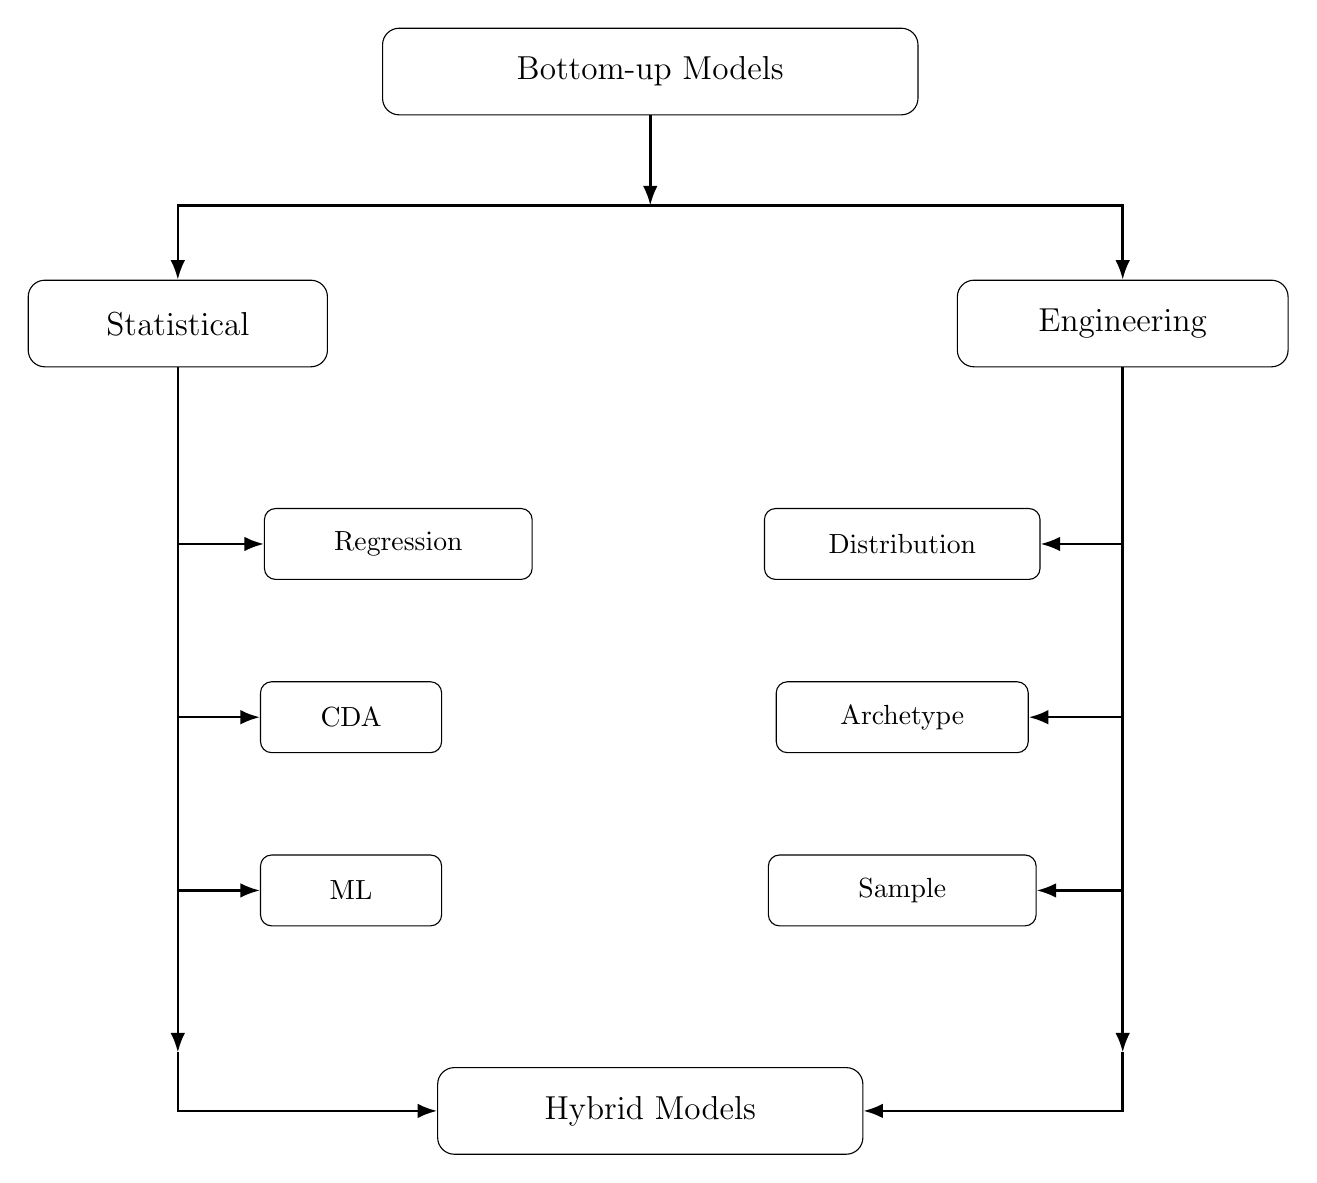
\begin{tikzpicture}[
    >=Latex,
    line/.style={draw, -Latex, line width=0.9pt},
    box/.style={
        draw,
        rounded corners=6pt,
        align=center,
        minimum height=11mm,
        inner sep=5pt,
        font=\large
    },
    smallbox/.style={
        draw,
        rounded corners=4pt,
        align=center,
        minimum height=9mm,
        inner sep=4pt,
        font=\normalsize
    }
]
% Top node
\node[box, minimum width=6.8cm] (top) at (0,0) {Bottom-up Models};
% Main branches
\node[box, minimum width=3.8cm] (stat) at (-6,-3.2) {Statistical};
\node[box, minimum width=4.2cm] (eng)  at ( 6,-3.2) {Engineering};
% Vertical trunks
\coordinate (split) at (0,-1.7);
\coordinate (statTop) at (-6,-1.7);
\coordinate (engTop)  at ( 6,-1.7);
% Statistical children
\node[smallbox, minimum width=3.4cm] (reg) at (-3.2,-6.0) {Regression};
\node[smallbox, minimum width=2.3cm] (cda) at (-3.8,-8.2) {CDA};
\node[smallbox, minimum width=2.3cm] (ml)  at (-3.8,-10.4) {ML};
% Engineering children
\node[smallbox, minimum width=3.5cm] (dist) at (3.2,-6.0) {Distribution};
\node[smallbox, minimum width=3.2cm] (arch) at (3.2,-8.2) {Archetype};
\node[smallbox, minimum width=3.4cm] (clust) at (3.2,-10.4) {Sample};
% Hybrid node
\node[box, minimum width=5.4cm] (hyb) at (0,-13.2) {Hybrid Models};
% Top connections
\draw[line] (top.south) -- (split);
\draw[line] (split) -| (stat.north);
\draw[line] (split) -| (eng.north);
% Statistical trunk and branches
\draw[line] (stat.south) -- ++(0,-8.7) coordinate (statBottom);
\draw[line] (-6,-6.0) -- (reg.west);
\draw[line] (-6,-8.2) -- (cda.west);
\draw[line] (-6,-10.4) -- (ml.west);
% Engineering trunk and branches
\draw[line] (eng.south) -- ++(0,-8.7) coordinate (engBottom);
\draw[line] (6,-6.0) -- (dist.east);
\draw[line] (6,-8.2) -- (arch.east);
\draw[line] (6,-10.4) -- (clust.east);
% Convergence to hybrid
\draw[line] (statBottom) |- (hyb.west);
\draw[line] (engBottom)  |- (hyb.east);
\end{tikzpicture}%
}
\vspace*{\fill}
\caption{Schematic overview of bottom-up modelling approaches.}
\label{fig:bottom_up_hierarchy}
\end{figure}


\pagebreak
% \section{Renewable Energy Communities}
% %  [needs more details, studies, results, situation in belgium...; but maybe wait with this section]
% % Define, map out, relate to residential energy demand modelling.
% Renewable Energy Communities (RECs) are legally recognized, democratically governed groups of local actors that collectively produce, consume, share and manage renewable energy for mutual environmental, economic and social benefit. Members may include households, small businesses, local authorities and other organizations. RECs aim to optimize local use of renewable energy, reduce reliance on fossil fuels, and provide services like demand flexibility and energy efficiency \cite{EnergyCommunity2026}.

% The following features can be assigned to RECs \cite{EnergyCommunity2026, corasanitiRenewableEnergyCommunities2025, EnergyCommunities}:
% \begin{itemize}
%     \item Open, voluntary participation: Members join by choice and share decision-making.
%     \item Local co-ownership and control: Members located near renewable generation assets have effective control.
%     \item Collective production and consumption: Members jointly produce, manage, and use renewable energy.
%     \item Environmental/economic benefits: RECs are structured to deliver local social or economic benefits (e.g., lower bills, local jobs). 
% \end{itemize}

% Corasaniti et al. \cite{corasanitiRenewableEnergyCommunities2025} describe RECs as “an innovative model for energy production, consumption, and sharing,” emphasizing decentralization and participation as defining aspects


% \subsection{Relationship with Residential Energy Demand}
% RECs intersect with residential demand in several fundamental ways \cite{ercoliDemandResponseRenewable2025, EnergyCommunities, corasanitiRenewableEnergyCommunities2025}. 

% \subsubsection*{Balancing load generation demand}
% Household electricity use often does not naturally align with renewable generation (e.g., PV output peaks midday while demand peaks at night). Effective REC operation requires detailed analysis of residential load profiles and strategies to adjust consumption patterns or storage use.
% \subsubsection*{Demand-side management}
% Demand flexibility techniques (e.g., shifting appliance use to times of high local generation) are central to REC performance. Ercoli et al. \cite{ercoliDemandResponseRenewable2025} show that coordinated demand response within a REC can meaningfully increase solar self-consumption and reduce community electricity costs.

% \subsubsection*{Residential load forecasting}
% Recent work uses machine learning to map hourly residential load profiles for REC planning and optimization, enabling better alignment between community supply and individual demand patterns.

% \subsubsection*{Residential self-consumption maximisation}
% Evaluated strategies \cite{hussainEnhancingRenewableEnergy2024} include:
% \begin{itemize}
%     \item Community storage shared across households to capture midday PV generation.
%     \item Internal energy trading among community members to increase local use of renewables.
% \end{itemize}


% \subsection{Residential Benefits}
% There are residential-level benefits tied to RECs \cite{ercoliDemandResponseRenewable2025, EnergyCommunities, corasanitiRenewableEnergyCommunities2025}:
% \begin{itemize}
%     \item Reduced electricity costs through localized pricing and self-consumption.
%     \item Enhanced energy autonomy for households, reducing dependence on distant generation.
%     \item Flexibility and demand management that can smooth peak loads and reduce grid stress.
%     \item Local economic and social benefits, including job creation and community engagement.
% \end{itemize}








% %%%%%%%% VERSION 1 %%%%%%%%

% % \section{Energy Demand}
% % The residential energy sector is undergoing rapid structural transformation driven by electrification and decarbonization. The deployment of electric heat pumps (HPs) as replacements for fossil-based heating systems and the accelerated adoption of electric vehicles (EVs) are fundamentally altering both the magnitude and temporal structure of the electricity demand. Unlike traditional household plug loads, these technologies introduce large, weather-dependent, and behaviour-sensitive electrical loads into the grid.

% % For example, air-to-water heat pumps exhibit strong performance variability between rated and in-use conditions, leading to discrepancies between expected and realized electricity consumption \cite{OHegarty2022_AWHPPerformanceGap, lammle_performance_2022}. Similarly, EV charging introduces high-power, temporally clustered loads that are driven by mobility behaviour rather than thermal demand dynamics (\cite{lekhel_generic_2025}). Therefore, the interaction between heating electrification and transport electrification creates new peak-load conditions, alters diversity factors, and increases system stress at the distribution levels.

% % This transformation implies that traditional aggregated load models are no longer sufficient. Electrified residential demand exhibits strong intra-day variability, coincidence effects, and stochastic user-dependent behaviour, necessitating bottom-up modelling approaches capable of resolving high-frequency dynamics.


% % \subsection{Renewable Energy Communities}

% % Renewable Energy Communities (RECs) introduce a new operational layer to residential demand modelling. In these systems, \textit{prosumers} collectively manage generation, storage, and demand to increase self-consumption and minimize grid interaction. Accurate forecasting becomes essential not merely for predictive accuracy, but for operational value.

% % Data-driven demand forecasting in RECs has shown that model quality does not necessarily translate directly into improved operational outcomes (\cite{coignard_evaluating_2021}). The timing of forecast errors can significantly affect battery dispatch, fairness allocation, and self-sufficiency metrics. Therefore, load modelling must consider not only deterministic prediction but uncertainty characterization.

% % In electrified communities, heat pumps, EVs, and distributed PV systems interact dynamically. The temporal coincidence between heating demand and low solar generation, or EV charging and evening peak load, creates system-level sensitivities. These interactions require modelling frameworks capable of propagating uncertainty from household behaviour to community-level performance.

% % \subsection{Importance of High-Resolution Demand Modelling}

% % High-resolution demand modelling is essential to capture diversity factors, switching behavior, and intra-hour variability. Classic bottom-up approaches have demonstrated that minute-level or sub-hourly resolution significantly improves realism compared to hourly aggregation (\cite{Richardson2010_DomesticHighRes, thorve_high_2023}).

% % Stochastic activity-based models translate occupant behavior into appliance activation patterns and resulting load profiles (\cite{Widén2009_StochasticActivity}). These approaches preserve diversity across dwellings and reduce artificial synchronization effects, which are common in deterministic scheduling models.

% % Similarly, stochastic bottom-up heating models capture variability in space heating and domestic hot water consumption, particularly under weather-driven conditions (\cite{Fischer2016_StochasticBottomUpHeatDHW}). High-resolution digital twin datasets further demonstrate the feasibility of generating large-scale disaggregated residential demand time series (\cite{thorve_high_2023}).

% % At city scale, two-step forecasting approaches combine building archetypes with statistical prediction layers to scale bottom-up modelling to urban contexts (\cite{yu_two-step_2018, frayssinet_modeling_2018}). However, these models often rely on deterministic building physics or averaged behavioral assumptions.


% % The increasing penetration of flexible electrified loads makes high-temporal resolution not optional but structurally necessary for capturing peak dynamics, rebound effects, and control opportunities.

% % \subsection{Deterministic Versus Stochastic Modelling Paradigms}

% % Traditional deterministic bottom-up models simulate appliance operation, heating loads, and occupancy schedules based on fixed or rule-based assumptions (\cite{Paatero2006_LoadProfileModel, subbiah_energy_2017}). While physically interpretable, such approaches risk underestimating variability and correlation structures inherent in real-world demand.

% % In contrast, stochastic models explicitly incorporate probabilistic representations of occupant behavior, appliance activation, and thermal response. Occupancy sequence generation methods produce realistic temporal patterns that better replicate empirical distributions (\cite{Aerts2017_RealisticOccupancySequences, rouleau_unified_2019}). Second-order thermal network models introduce dynamic thermal inertia effects that respond probabilistically to weather and control signals (\cite{wang_development_2022}).

% % Stochastic frameworks are particularly important under climate change and long-term electrification scenarios. Climate-induced shifts in heating and cooling demand require modelling approaches that integrate probabilistic weather inputs with building stock evolution (\cite{elnagar_modeling_2021}). Spatially explicit bottom-up stock models further highlight the importance of capturing heterogeneity at regional scale (\cite{dalonzo_bottom-up_2019}).

% % The paradigm shift from deterministic to stochastic modelling reflects a broader transition: from average load estimation toward uncertainty-aware energy system analysis. Electrified residential demand is no longer a static profile but a probabilistic process shaped by occupant behaviour, technology adoption, and climate variability.

% % In the context of RECs and grid-interactive buildings, modelling frameworks must therefore transition from deterministic schedule generation to fully stochastic, bottom-up representations capable of uncertainty propagation across scales.


% % \section{Modelling Paradigms in Residential Energy Demand}

% % \subsection{Top-Down Statistical Approaches}

% % Top-down modelling approaches represent residential energy demand at an aggregated level, typically at regional, national, or utility scale. These methods rely on historical consumption data and explanatory variables such as weather indicators, socio-economic factors, or macroeconomic trends. Regression-based models, autoregressive integrated moving average (ARIMA) formulations, and machine learning predictors are frequently applied in this context (\cite{muratori_highly_2013, Hong2016}).

% % Forecasting-oriented top-down approaches are particularly common in short-term load forecasting (STLF), where the objective is to predict aggregate demand over horizons ranging from hours to days. Data-driven forecasting models for Local Energy Communities (LECs) demonstrate the operational relevance of accurate demand prediction (\cite{coignard_evaluating_2021}). At city scale, hybrid forecasting frameworks combine statistical prediction layers with archetype-based aggregation to improve predictive performance (\cite{yu_two-step_2018}).

% % The primary limitation of top-down approaches lies in their lack of appliance-level or occupant-level granularity. Because they operate on aggregated consumption signals, they cannot explicitly represent appliance activation, occupant behavior, or technology adoption dynamics. Consequently, these models offer limited insight into flexibility potentials, electrification impacts, or load-shifting mechanisms at household level. They are therefore unsuitable for detailed demand response analysis or bottom-up uncertainty propagation.


% % \subsection{Deterministic Bottom-Up Physical Models}

% % Deterministic bottom-up models simulate residential energy demand by explicitly modelling individual appliances, end-uses, and building thermal behavior. Appliance-level electricity demand is generated by assigning rated power values and predefined operation schedules, often based on empirical averages or rule-based assumptions (\cite{Paatero2006_LoadProfileModel}). High-resolution domestic electricity models further incorporate appliance ownership statistics and duty-cycle representations to reproduce minute-level demand fluctuations (\cite{Richardson2010_DomesticHighRes, thorve_high_2023}).

% % Weather-driven generators extend this framework by coupling end-use demand to climatic inputs. For heating and domestic hot water (DHW), deterministic reduced-order thermal models—such as resistance-capacitance (RC) networks—are commonly employed. Reduced-order 5R1C building models capture thermal mass, envelope heat transfer, and ventilation losses while maintaining computational tractability (\cite{Fischer2016_StochasticBottomUpHeatDHW, Reynders2014_ModelComplexity}). At regional scale, spatially explicit stock models apply deterministic archetype simulations across heterogeneous building inventories (\cite{dalonzo_bottom-up_2019}).

% % The principal strength of deterministic bottom-up models is interpretability. Each load component can be traced back to a physical mechanism, allowing direct linkage between technology adoption (e.g., heat pumps) and resulting demand changes. However, these models typically rely on fixed schedules or averaged behavioral assumptions. Uncertainty in occupant behavior, appliance timing, and climate variability is not explicitly propagated. As electrification increases stochastic variability, purely deterministic representations risk underestimating peak coincidence and diversity effects.


% % \subsection{Time-Use \& Behavioural Bottom-Up Models}

% % Time-use and behavioural models introduce occupant activity as the central driver of residential energy demand. These approaches convert diary-based time-use surveys into activity sequences, which are subsequently mapped to appliance activation probabilities (\cite{Widén2009_StochasticActivity}). Appliance switch-on events are often modelled using probabilistic rules conditioned on occupancy state, time of day, and appliance ownership.

% % A key contribution of behavioural bottom-up models is the preservation of diversity factors across dwellings. By generating independent yet statistically consistent activity patterns, artificial synchronization effects are avoided. High-resolution occupancy models further enable the creation of realistic heating load profiles that integrate presence-dependent internal gains and thermostat interactions (\cite{Buttitta2020_HighResOccupancyHeating}). Methods for generating realistic domestic occupancy sequences improve the temporal realism of simulated demand patterns (\cite{Aerts2017_RealisticOccupancySequences, rouleau_unified_2019}).

% % Despite incorporating probabilistic activation mechanisms, many time-use based models remain only weakly stochastic. Transition probabilities are often derived directly from survey frequencies without dynamic state-dependent adaptation. Furthermore, correlations between appliances and multi-occupant interactions are only partially captured. Consequently, while these models represent a substantial improvement over deterministic schedules, they often lack fully dynamic stochastic state evolution and uncertainty quantification.


% % \subsection{Data-Driven Archetyping \& Clustering}

% % Data-driven archetyping approaches rely on clustering techniques to segment load profiles into representative consumption patterns. Principal Component Analysis (PCA) is frequently employed for dimensionality reduction, enabling the extraction of dominant temporal load features prior to clustering. Cluster validation indices, such as silhouette score or Davies–Bouldin index, guide the selection of optimal cluster numbers.

% % Clustering smart-meter datasets reveals distinct daily load-shape archetypes associated with dwelling type, socio-economic variables, or occupancy patterns (\cite{McLoughlin2012_ClusteringSmartMeters}). These archetypes are useful for demand segmentation, tariff design, and scenario analysis. At larger scales, clustering can serve as a calibration target for bottom-up models by ensuring that simulated load profiles reproduce empirical distributional characteristics.

% % However, purely data-driven segmentation methods do not embed physical causality or occupant mechanisms. They describe patterns without explaining underlying processes. While valuable for validation and benchmarking, clustering-based models cannot independently generate physically consistent synthetic demand without integration into bottom-up frameworks.

% % Together, these four paradigms—top-down statistical models, deterministic physical bottom-up models, behavioural bottom-up approaches, and data-driven archetyping—form the methodological landscape of residential energy demand modelling. Each addresses specific aspects of the modelling challenge, yet none independently provides a fully uncertainty-aware, high-resolution, stochastic representation suitable for electrified and community-integrated energy systems.


% % \section{High-Resolution \& Digital Twin Approaches}

% % High-resolution and digital twin approaches aim to generate residential demand time series that preserve fine-grained temporal structure, appliance-level dynamics, and heterogeneity across households. These methods are increasingly relevant in electrified contexts because sub-hourly variability and coincidence effects strongly influence peak demand, flexibility potential, and the operation of LECs.

% % \subsection{Large-Scale Digital Twin Datasets}

% % A recent line of work focuses on generating large-scale digital twin datasets that provide disaggregated residential energy use time series at scale. Thorve et al. propose a bottom-up approach to generate hourly digital twin data of disaggregated residential energy use, enabling the creation of large synthetic populations for downstream analytics and forecasting research (\cite{thorve_high_2023}). Digital twin datasets offer a structured representation of residential end uses, facilitating scenario analysis (e.g., technology adoption, electrification) while remaining computationally tractable compared to full physics-based simulation of each dwelling.

% % These datasets are typically validated by comparing aggregate statistics (daily/seasonal load shapes, annual consumption) and distributional properties across the synthetic population. The advantage of the digital twin paradigm is that it supports large-sample simulation studies and uncertainty exploration. A limitation, particularly at hourly resolution, is that intra-hour variability and switching dynamics may be smoothed out, which can be critical for modelling flexibility and peak coincidence in highly electrified households.

% % \subsection{UK and Danish One-Minute High-Resolution Models}

% % High-resolution bottom-up models at one-minute resolution were developed to capture appliance switching behavior and realistic diversity in domestic electricity demand. The UK high-resolution domestic load modelling tradition is exemplified by the stochastic demand model of Richardson et al., which generates appliance-level switching events and produces realistic minute-scale profiles suitable for demand simulations and technology assessments (\cite{Richardson2010_DomesticHighRes}). Similarly, Danish high-resolution household electricity demand models target minute-level realism while preserving heterogeneity across households, with emphasis on reproducing observed diversity factors and temporal patterns (\cite{thorve_high_2023}).

% % These approaches are motivated by the need to represent short-lived, high-power events (e.g., kettles, cooking appliances, EV charging ramp-ups) and the clustering of events during morning and evening routines. By using probabilistic switching rules and activity-driven triggers, one-minute models can reproduce empirical peak distributions more realistically than hourly models.

% % \subsection{Within-Home Correlation and Behavioural Coupling}

% % A critical advantage of high-resolution behavioural bottom-up models is their ability to preserve within-home correlations. Real households exhibit correlated appliance use because activities and occupant presence drive multiple appliances jointly (e.g., cooking correlates with lighting and entertainment; showering correlates with DHW and ventilation). Activity-based stochastic approaches explicitly address this by modelling sequences of domestic activities and mapping them to appliance activation events (\cite{Widén2009_StochasticActivity}). Occupancy-based models similarly preserve coupling between presence, internal gains, and heating demand, which becomes essential for integrated electricity--heat simulations (\cite{Buttitta2020_HighResOccupancyHeating}).

% % In contrast, models that sample appliances independently often reproduce marginal statistics but fail to replicate correlation structures, leading to unrealistic simultaneity patterns. Preserving within-home correlation is therefore not only a matter of realism; it directly affects peak coincidence, load shifting opportunities, and the reliability of flexibility estimates.

% % \subsection{Diversity Scaling and Population Aggregation}

% % A major methodological challenge is scaling high-resolution models from a single dwelling to populations (neighbourhoods, communities, cities) while preserving diversity. Diversity scaling refers to ensuring that aggregate demand does not grow linearly with household count due to coincident peak reduction through heterogeneity. High-resolution models typically incorporate diversity implicitly through stochastic activity generation and household-specific parameters, which reduces synchronization effects when aggregating multiple simulated dwellings (\cite{Richardson2010_DomesticHighRes, Widén2009_StochasticActivity}).

% % Digital twin approaches offer a complementary strategy by generating large synthetic populations with parameter heterogeneity; however, if temporal patterns are not sufficiently diverse or if resolution is too coarse, peak coincidence may still be distorted (\cite{thorve_high_2023}). For Local Energy Communities, diversity scaling is especially important because community-level metrics (self-consumption, peak import, storage sizing) are sensitive to the distribution and simultaneity of loads.

% % \subsection{Validation Metrics Used in High-Resolution Modelling}

% % Validation of high-resolution and digital twin models typically goes beyond pointwise error metrics. Common metrics include comparisons of mean daily profiles, load duration curves, peak demand distributions, and diversity factors at different aggregation levels. Time-series similarity measures may be used at household level, while distributional checks (e.g., quantiles of power, peak coincidence ratios) are critical at population level.

% % For models intended to support control and REC operation, validation often also includes assessing whether synthetic demand reproduces key operational outcomes (e.g., peak import timing, storage dispatch patterns) when embedded in an energy management simulation (\cite{coignard_evaluating_2021}). Overall, high-resolution and digital twin approaches emphasize that realism in residential demand modelling is fundamentally multi-criteria: capturing averages is insufficient if variability, correlation, and diversity scaling are misrepresented.

% % In summary, high-resolution and digital twin approaches provide the methodological basis for generating realistic residential demand time series under electrification. One-minute behavioural models excel at capturing switching dynamics and within-home correlations, while digital twin datasets enable large-scale population modelling. Their integration into uncertainty-aware frameworks remains a central step toward stochastic bottom-up modelling suitable for climate uncertainty and REC applications.


% % \section{Model Validation \& Calibration Strategies}

% % Robust validation and calibration are central challenges in residential energy demand modelling. As model complexity increases—through higher temporal resolution, behavioural representation, or spatial scaling—traditional pointwise error metrics become insufficient to evaluate model performance. This section reviews commonly used validation strategies and highlights limitations that motivate probabilistic calibration approaches.

% % \subsection{Pointwise Error Metrics: RMSE and MAPE}

% % Root Mean Square Error (RMSE) and Mean Absolute Percentage Error (MAPE) are widely used to evaluate model performance against measured demand data. These metrics quantify the deviation between simulated and observed load time series, typically at hourly or daily resolution.

% % Forecasting-oriented studies frequently rely on RMSE or MAPE to compare model architectures (\cite{coignard_evaluating_2021}). While these metrics provide intuitive measures of average prediction accuracy, they are sensitive to aggregation level and may obscure structural mismatches. For example, a model can achieve low RMSE while misrepresenting peak timing or diversity effects, particularly when evaluated at aggregate scale.

% % Moreover, percentage-based metrics such as MAPE are unstable when applied to low-load periods and do not adequately reflect operational consequences in electrified systems where peak events dominate infrastructure constraints.

% % \subsection{Diversity Factor}

% % The diversity factor quantifies the degree to which aggregated peak demand is reduced relative to the sum of individual peak demands. It is a critical validation metric for bottom-up models intended to represent multiple households. High-resolution stochastic models explicitly aim to reproduce realistic diversity effects through independent yet statistically consistent behavioural patterns (\cite{Richardson2010_DomesticHighRes, Widén2009_StochasticActivity}).

% % Failure to reproduce empirical diversity factors leads to overestimated peak demand when aggregating synthetic households. Deterministic scheduling models, in particular, risk artificial synchronization, resulting in unrealistic simultaneity of appliance use. Therefore, diversity factor validation is essential when scaling from single-dwelling simulations to neighbourhood or community-level analyses.

% % \subsection{Load Duration Curves and Distributional Validation}

% % Load duration curves (LDCs) provide a complementary validation tool by assessing the distribution of demand values independent of temporal order. Comparing simulated and measured LDCs reveals whether a model correctly captures the frequency and magnitude of high-load events.

% % Distributional validation is especially important for electrified households, where rare but extreme events (e.g., simultaneous heat pump operation and EV charging) drive network constraints. While RMSE may indicate good average fit, mismatches in the upper tail of the load distribution can remain undetected unless LDC or quantile-based metrics are examined.

% % \subsection{Cluster Validation Indices}

% % When models are calibrated against archetypal load shapes derived from clustering, Cluster Validation Indices (CVIs) such as silhouette score or Davies–Bouldin index are employed to assess clustering quality. Smart-meter based segmentation studies demonstrate that clustering can reveal characteristic demand patterns associated with dwelling type or socio-economic variables (\cite{McLoughlin2012_ClusteringSmartMeters}).

% % In bottom-up modelling, archetypes derived through clustering can serve as calibration targets. However, CVIs assess internal cluster coherence rather than physical realism. A model calibrated to reproduce cluster centroids may match statistical structure while still lacking causal interpretability.

% % \subsection{Limitations of Current Calibration Approaches}

% % Most residential bottom-up models rely on deterministic parameter tuning or heuristic calibration. Appliance usage frequencies, thermal parameters, or occupancy probabilities are adjusted until aggregate metrics (annual consumption, average daily profile) align with empirical data. Such approaches often ignore parameter uncertainty and correlations between inputs.

% % Reduced-order building models illustrate this challenge: parameter identification quality depends strongly on the accuracy of input signals and measurement noise (\cite{Reynders2014_ModelComplexity}). Deterministic calibration yields a single “best-fit” parameter set, but does not quantify uncertainty in thermal resistance, capacitance, or behavioural transition probabilities.

% % Similarly, digital twin datasets and stochastic behavioural models are typically validated using descriptive statistics without formal inference of parameter distributions (\cite{thorve_high_2023}). As electrification increases structural uncertainty—through technology adoption variability, behavioural adaptation, and climate effects—deterministic calibration becomes increasingly inadequate.

% % \subsection{Toward Probabilistic Calibration and Bayesian Inference}

% % Probabilistic calibration frameworks, particularly Bayesian approaches, offer a principled method to quantify parameter uncertainty and propagate it through the model. Rather than estimating a single parameter vector, Bayesian calibration infers posterior distributions conditioned on observed data. This enables uncertainty intervals for predicted demand trajectories and peak events.

% % In electrified and REC-integrated systems, uncertainty quantification is not merely an academic refinement but a practical necessity. Forecasting studies demonstrate that operational outcomes (e.g., storage dispatch, self-consumption rates) depend strongly on the timing and distribution of errors rather than only on mean accuracy (\cite{coignard_evaluating_2021}). Stochastic demand representations therefore directly influence control performance and infrastructure planning.

% % When demand is modelled as a stochastic process rather than a deterministic schedule, uncertainty propagation enables evaluation of worst-case peak coincidence, flexibility potential under behavioural variability, and resilience under climate perturbations (\cite{elnagar_modeling_2021}). Bayesian calibration further allows integration of heterogeneous data sources, such as smart-meter time series, occupancy surveys, and field monitoring of heat pumps (\cite{OHegarty2022_AWHPPerformanceGap}).

% % In summary, while traditional validation metrics such as RMSE, MAPE, diversity factors, and load duration curves remain essential diagnostic tools, they are insufficient for uncertainty-aware electrified system modelling. A shift toward probabilistic calibration—grounded in Bayesian inference—enables formal uncertainty quantification and more robust control-oriented assessment in stochastic bottom-up residential energy demand frameworks.


% % \section{Identified Research Gaps}

% % Despite substantial progress in residential energy demand modelling, several structural limitations persist across modelling paradigms. These limitations become increasingly critical under large-scale electrification, climate variability, and the operational requirements of Local Energy Communities.

% % \subsection{Deterministic Bias}

% % A recurring limitation across bottom-up and stock-level models is deterministic bias. Even when models incorporate behavioural rules or probabilistic activation frequencies, many implementations ultimately rely on fixed parameter sets, averaged schedules, or single “best-fit” thermal representations (\cite{Paatero2006_LoadProfileModel, Fischer2016_StochasticBottomUpHeatDHW}). 

% % Deterministic reduced-order building models are often calibrated to reproduce annual consumption or mean daily profiles, but they neglect uncertainty in envelope parameters, occupant adaptation, and control behaviour (\cite{Reynders2014_ModelComplexity}). As electrification increases the sensitivity of peak demand to coincident events, deterministic representations systematically underestimate variability and tail risk. This bias becomes particularly problematic when assessing network constraints or storage sizing.

% % \subsection{Limited Stochastic Occupancy Modelling}

% % While time-use and activity-based models introduce probabilistic appliance activation (\cite{Widén2009_StochasticActivity}), many frameworks treat occupancy transitions as static probabilities derived directly from survey frequencies. Dynamic state evolution, inter-occupant interactions, and adaptive behaviour remain insufficiently modelled.

% % Occupancy sequence generation methods improve realism (\cite{Aerts2017_RealisticOccupancySequences, rouleau_unified_2019}), yet integration of occupancy as a formal stochastic process—e.g., state-dependent Markov chains with explicit transition matrices—is rarely embedded consistently within integrated electricity--heat models. As a result, correlations between occupancy, appliance usage, heating demand, and EV charging are only partially captured.

% % In electrified dwellings, occupancy patterns directly influence heat pump cycling, domestic hot water usage, and discretionary loads. Limited stochastic occupancy modelling therefore constrains the ability of current models to represent behavioural heterogeneity and peak coincidence under real-world conditions.

% % \subsection{Lack of Uncertainty Propagation to REC Metrics}

% % Forecasting studies in Local Energy Communities demonstrate that prediction quality does not translate linearly into operational value (\cite{coignard_evaluating_2021}). However, most bottom-up demand generators provide deterministic time series without uncertainty envelopes. Consequently, uncertainty is not propagated into community-level performance metrics such as:

% % \begin{itemize}
% %   \item self-consumption ratio,
% %   \item peak import/export,
% %   \item storage dispatch patterns,
% %   \item fairness allocation among prosumers.
% % \end{itemize}

% % Digital twin datasets and high-resolution generators reproduce statistical structure (\cite{thorve_high_2023}), yet rarely quantify how behavioural or climatic uncertainty affects REC outcomes. This gap limits the ability to perform risk-aware planning and to evaluate system robustness under stochastic demand fluctuations.

% % \subsection{Limited Probabilistic Calibration}

% % Calibration practices remain predominantly deterministic and heuristic. Parameter tuning is typically conducted to match aggregate statistics or minimize RMSE, without formal inference of parameter distributions. Thermal network identification studies highlight sensitivity to measurement noise and input accuracy (\cite{Reynders2014_ModelComplexity}), yet uncertainty bounds are seldom reported.

% % Without probabilistic calibration, model outputs cannot provide credible intervals for peak demand, diversity factors, or seasonal variability. This limitation becomes particularly critical when modelling climate change impacts on building energy demand (\cite{elnagar_modeling_2021}), where both exogenous (weather) and endogenous (behavioural) uncertainties interact.

% % Overall, existing approaches lack a unified framework that simultaneously models behavioural stochasticity, climate uncertainty, and parameter uncertainty while propagating these effects to system-level performance indicators.


\mode<all> % do not remove
    \chapterOrPart{Methodology}\label{ch:materialsmethods}

\section{Methodological Scope}
\label{sec:methodological_scope}
 
The objective of this work is to quantify how Belgian residential energy demand may evolve under changing climate forcing and changing household technology stocks, while preserving household-level behavioural variability. This requires a model that resolves dwellings and end-uses, responds physically to weather, and keeps climate, technology, and stochastic variation separable in the results.\footnote{Throughout this section, the modelling paradigm is positioned against the residential demand modelling literature surveyed by \textcite{swan_modeling_2009,kavgicReviewBottomupBuilding2010, Allegrini2015}.} \Cref{fig:scope_taxonomy} situates the chosen paradigm against the broader taxonomy of residential demand models.
 
% ---------------------------------------------------------------------
% Figure: taxonomy of residential demand models with our position
% ---------------------------------------------------------------------
\begin{figure}[ht]
  \centering
  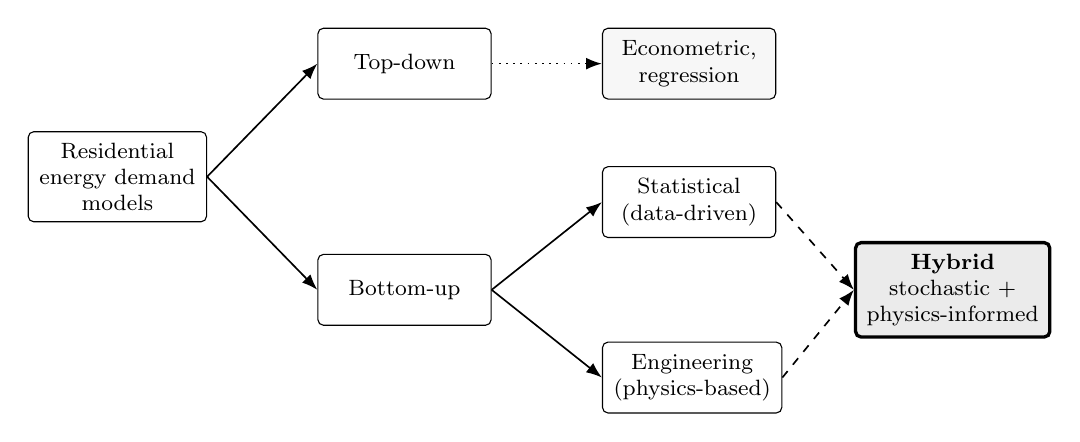
\begin{tikzpicture}[
      every node/.style={font=\footnotesize, align=center},
      box/.style={draw, rounded corners=2pt, inner sep=4pt,
                  minimum height=9mm, minimum width=22mm},
      pick/.style={box, fill=black!8, very thick},
      arrow/.style={-{Latex[length=2mm]}, semithick},
      node distance=10mm and 14mm,
  ]
    % Column 1: root
    \node[box] (root) {Residential\\energy demand\\models};
 
    % Column 2: top-down / bottom-up (stacked vertically)
    \node[box, above right=4mm and 14mm of root] (td) {Top-down};
    \node[box, below right=4mm and 14mm of root] (bu) {Bottom-up};
    \draw[arrow] (root.east) -- (td.west);
    \draw[arrow] (root.east) -- (bu.west);
 
    % Column 3: leaf families
    \node[box, right=14mm of td, fill=black!3]
      (td_ex) {Econometric,\\regression};
    \node[box, above right=2mm and 14mm of bu]  (stat) {Statistical\\(data-driven)};
    \node[box, below right=2mm and 14mm of bu]  (eng)  {Engineering\\(physics-based)};
    \draw[arrow, dotted] (td.east) -- (td_ex.west);
    \draw[arrow] (bu.east) -- (stat.west);
    \draw[arrow] (bu.east) -- (eng.west);
 
    % Column 4: hybrid pick (vertically centred between stat and eng)
    \node[pick, right=14mm of bu, xshift=32mm]
      (hyb) {\textbf{Hybrid}\\stochastic +\\physics-informed};
    \draw[arrow, dashed] (stat.east) -- (hyb.west);
    \draw[arrow, dashed] (eng.east)  -- (hyb.west);
  \end{tikzpicture}
  \caption{Position of the proposed model within the residential demand modelling taxonomy.}
  \label{fig:scope_taxonomy}
\end{figure}
The model is bottom-up (per-dwelling, per-end-use) and combines a stochastic occupancy/behaviour layer with a physics-informed thermal and technology layer, following the hybrid family introduced by \textcite{Capasso1994,Richardson2010_DomesticHighRes,McKenna2015}. A bottom-up formulation is required because the thesis compares technology substitution, weather sensitivity, and cohort peak coincidence rather than only aggregate annual demand.


\subsection{Hybrid Approach}
\label{sec:hybrid_approach}
 
This work adopts a hybrid formulation in the sense of \textcite{Capasso1994}, refined by the CREST family of models \cite{Richardson2010CRESTElectricity,McKenna2015} and the behavioural-physics couplings reviewed by \textcite{Sandels2016,DOca2017}. Concretely:
\begin{itemize}[leftmargin=1.2em, itemsep=2pt, topsep=2pt]
  \item Stochasticity is introduced at the \emph{behavioural} layer, through a probabilistic occupancy and activity model that drives the metabolic, lighting, appliance, cooking, and DHW end-uses. This recovers between-household diversity, plausible coincidence factors, and load-shape variability without prescribing a single average profile.
  \item Physics is introduced at the \emph{thermal} and \emph{system} layers, through a reduced-order (lumped-capacitance) building thermal balance and through temperature-dependent conversion efficiencies. This guarantees that space heating and electrified heating respond mechanistically to outdoor temperature and solar gains, which is the channel through which \hyperref[sec:climateScenariosFramework]{climate scenarios} act.
\end{itemize}
 
This combination is the minimum modelling content required for the research question: weather sensitivity comes from the physical layers, while diversity and coincidence come from the stochastic layers.


\subsection{Base Framework}
\label{sec:base_framework}
 
The resulting framework is therefore a \emph{stochastic, physics-informed, bottom-up} model of residential energy demand. Its data contract follows the canonical pipeline used in the model implementation:
 
\begin{equation}\label{eq:dataContract}
\begin{split}
  \underbrace{\text{InputDataset}}_{\text{dwelling, weather, tech}}
  &\to
  \underbrace{\text{PreparedForcing}}_{\text{time-aligned drivers}}
  \to
  \underbrace{\text{PhysicsState}}_{\text{thermal balance}}\\
  &\to
  \underbrace{\text{ControlState}}_{\text{thermostat, deadband}}
  \to
  \underbrace{\text{SystemState}}_{\text{carriers, PV, EV, grid}}
  \to
  \underbrace{\text{ModelOutputs}}_{\text{kWh, kW, HDD, etc.}}
\end{split}
\end{equation}
 
Each block is a typed interface, so the boundary between behaviour, physics, control, and systems remains auditable. The same pipeline is reused across deterministic annual runs, stochastic cohort simulations, and scenario-tree experiments; only the configuration changes.


\subsection{System Boundary}
\label{sec:system_boundary}
 
A defensible scope requires an explicit boundary. \Cref{fig:system_boundary} summarises the boundary adopted in this work: climate forcing and technology assumptions enter as exogenous inputs; behaviour, physics, control, and systems are simulated endogenously; and the outputs are final energy per carrier, peak power, grid exchange, and comfort indicators.
 
% ---------------------------------------------------------------------
% Figure: explicit system boundary
% ---------------------------------------------------------------------
\begin{figure}[ht]
  \centering
  % \resizebox scales the whole picture (including its text) to \textwidth
  % so the diagram can never overflow horizontally.
  \resizebox{\textwidth}{!}{%
  \begin{tikzpicture}[
      every node/.style={font=\footnotesize, align=center},
      block/.style={draw, rounded corners=2pt, inner sep=3pt,
                    minimum height=8mm, minimum width=22mm},
      forcing/.style={block, fill=black!3},
      outblock/.style={block, fill=black!8},
      arrow/.style={-{Latex[length=2mm]}, semithick},
      node distance=6mm and 8mm,
  ]
    % --- Inside the boundary (placed first, boundary fits around them) ---
    \node[block]                    (ctrl) {Control};
    \node[block, right=of ctrl]     (phys) {Thermal balance};
    \node[block, right=of phys]     (sys)  {Energy systems};
    \node[block, above=5mm of phys] (occ)  {Occupancy \&\\ stochastic activity};
 
    \draw[arrow] (occ)  -- (phys);
    \draw[arrow] (ctrl) -- (phys);
    \draw[arrow] (phys) -- (sys);
 
    % --- Boundary box drawn AROUND the inner nodes via the `fit' library ---
    \node[draw, dashed, rounded corners=4pt, inner sep=5mm,
          fit=(occ)(ctrl)(phys)(sys)] (bnd) {};
    \node[anchor=south west, font=\footnotesize\itshape, inner sep=2pt,
          fill=white]
      at ([xshift=3mm,yshift=-0.4mm]bnd.north west)
      {\,System boundary: residential dwelling cohort\,};
 
    % --- Exogenous forcing (left, outside boundary) ---
    \node[forcing, left=10mm of ctrl]            (clim) {Climate forcing\\($T_{\text{out}}$, $G_{\text{sol}}$)};
    \node[forcing, below=3mm of clim, anchor=north west, xshift=0mm]
                                                 (tech) {Technology case};
    \draw[arrow] (clim.east) -- (ctrl.west);
    \draw[arrow] (tech.east) -| ([xshift=-3mm]sys.west) -- (sys.west);
 
    % --- Outputs (right, outside boundary) ---
    \node[outblock, right=10mm of sys] (kWh) {Final energy};
    \node[outblock, above=3mm of kWh]  (com) {Comfort \&\\overheating};
    \node[outblock, below=3mm of kWh]  (kW)  {Peak power\\\& grid exchange};
    \draw[arrow] (sys.east) -- (kWh.west);
    \draw[arrow] (sys.east) -- (com.west);
    \draw[arrow] (sys.east) -- (kW.west);
  \end{tikzpicture}}
  \caption{System boundary of the model.}
  \label{fig:system_boundary}
\end{figure}
 
The scope is the Belgian residential stock, represented through dwelling archetypes and household cohorts. Tertiary, industrial, and transport-sector loads are excluded; EVs enter only as residential charging at the dwelling meter. The model is non-spatial in the network sense, with all dwellings connected to one import/export boundary and climate forcing taken at the Uccle/Brussels reference point. Historical-weather runs use the hourly canonical configuration, while processed CORDEX leaves use their active forcing timestep. Final energy is reported for electricity, natural gas, fuel oil, and other configured heating carriers; primary-energy, emissions, and economic accounting are post-processing layers rather than simulator state.

 
% ---------------------------------------------------------------------
% Table: inclusions / exclusions
% ---------------------------------------------------------------------
\begin{table}[ht]
  \centering
  \footnotesize
  \caption{System boundary: explicit inclusions and exclusions.}
  \label{tab:scope_inclusions_exclusions}
  \begin{tabular}{@{}p{0.46\linewidth} p{0.46\linewidth}@{}}
    \toprule
    \textbf{Inside the boundary} & \textbf{Outside the boundary} \\
    \midrule
    Residential dwellings (per-archetype) &
      Tertiary, industrial, and transport sectors \\
    Stochastic occupancy and activity &
      Detailed agent-based household behaviour \\
    Reduced-order thermal balance &
      Multi-zone CFD or full building-physics simulation \\
    Temperature-dependent heat-pump COPs and conversion losses &
      Component-level HVAC dynamics, refrigerant cycles \\
    PV self-consumption and grid import/export at the dwelling meter &
      Distribution-network impedances, voltage, congestion \\
    Final-energy demand per carrier (electricity, gas, oil) &
      Primary energy, $\mathrm{CO_2}$ accounting \\
    Comfort and overheating indicators (CDD, exceedance hours) &
      Active cooling final-energy consumption \\
    Climate forcing via CORDEX RCP pathways &
      Probabilistic climate forecasts; ensemble downscaling beyond
      the configured GCM/RCM chain \\
    \bottomrule
  \end{tabular}
\end{table}


\subsection{Core Assumptions}
\label{sec:core_assumptions}
 
The load-bearing assumptions of the methodological scope are:
 
\begin{enumerate}[label=A\arabic*., leftmargin=2.2em, itemsep=2pt, topsep=2pt]
  \item \textbf{Single-zone thermal representation.} Each dwelling is modelled as one thermal zone with a lumped UA and thermal mass, consistent with reduced-order residential demand models \cite{Reynders2014_ModelComplexity,Bacher2011}. Inter-room dynamics, stack effects, and humidity are not resolved.
 
  \item \textbf{Independent households.} Households are conditionally
  independent given climate forcing and the technology case; there is no peer-effect or social-network coupling between dwellings. Cohort coincidence emerges from shared exogenous forcing and from the archetype/behaviour distributions.
 
  \item \textbf{No active cooling final energy.} Active cooling is not converted into electricity consumption; cooling pressure is reported only through CDD, indoor overheating hours, and excess-heat indicators.
 
  \item \textbf{No network constraints.} Voltage, congestion, and distribution losses are not modelled. Grid import and export are computed at the dwelling meter.
 
  \item \textbf{Deterministic climate forcing per leaf.} Each scenario leaf consumes one climate forcing file from one CORDEX GCM/RCM chain. RCP pathways are treated as conditional scenarios, not probabilistic forecasts, in line with \textcite{vanVuuren2011,IPCC2014}.
 
  \item \textbf{Technology cases are conditional.} Future technology stocks are counterfactual stocks, not calibrated adoption forecasts.
 
  \item \textbf{Stochasticity is reproducible.} Random draws for occupancy, archetype assignment, and parameter perturbations are controlled by integer seeds recorded in the run registry.
\end{enumerate}
 
The validation strategy in \Cref{sec:validation} pairs the model against macro-level Belgian residential carrier totals, synthetic load profiles (SLPs), and high-frequency KU Leuven and Fluvius smart-meter data. Future scenario leaves cannot be externally validated against observations and are therefore interpreted as conditional projections \cite{IPCC2021}.


\subsection{Scenario-tree System}
\label{sec:scenarioTreeSystem}
 
The scenario-tree layer defines each result as one \emph{leaf} of a four-dimensional tree, so the assumptions behind a number are explicit before that number is interpreted. \Cref{fig:scenario_tree} sketches the tree.
 
% ---------------------------------------------------------------------
% Figure: scenario tree
% ---------------------------------------------------------------------
\begin{figure}[ht]
  \centering
  % \resizebox enforces \textwidth as the hard maximum, so the figure
  % can never overflow the page regardless of its natural size.
  \resizebox{\textwidth}{!}{%
  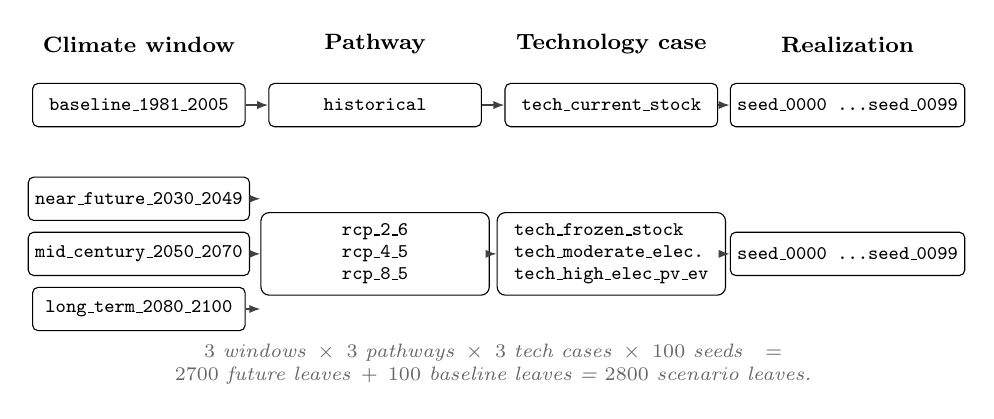
\begin{tikzpicture}[
      x=3cm, y=0.7cm,
      every node/.style={font=\scriptsize, align=center, inner sep=2.5pt},
      idbox/.style={draw, rounded corners=2pt,
                    font=\scriptsize\ttfamily,
                    minimum height=5.5mm, minimum width=2.7cm},
      groupbox/.style={draw, rounded corners=3pt,
                       font=\scriptsize\ttfamily, align=left,
                       inner sep=4pt, minimum width=2.9cm},
      brace/.style={decorate, decoration={brace, amplitude=4pt}},
      colhdr/.style={font=\footnotesize\bfseries},
      arrow/.style={-{Latex[length=1.4mm]}, semithick, draw=black!75},
  ]
    %% --- Column headers ---------------------------------------------
    \node[colhdr] at (0, 5.2) {Climate window};
    \node[colhdr] at (1, 5.2) {Pathway};
    \node[colhdr] at (2, 5.2) {Technology case};
    \node[colhdr] at (3, 5.2) {Realization};
 
    %% --- Baseline branch (top, one value per dimension) -------------
    \node[idbox] (W1) at (0, 4.1) {baseline\_1981\_2005};
    \node[idbox] (P1) at (1, 4.1) {historical};
    \node[idbox] (T1) at (2, 4.1) {tech\_current\_stock};
    \node[idbox] (R1) at (3, 4.1) {seed\_0000 \dots seed\_0099};
    \draw[arrow] (W1) -- (P1);
    \draw[arrow] (P1) -- (T1);
    \draw[arrow] (T1) -- (R1);
 
    %% --- Three future windows sharing one expansion -----------------
    \node[idbox] (W2) at (0,  2.4) {near\_future\_2030\_2049};
    \node[idbox] (W3) at (0,  1.4) {mid\_century\_2050\_2070};
    \node[idbox] (W4) at (0,  0.4) {long\_term\_2080\_2100};
 
    % Pathway group (lists the 3 RCPs)
    \node[groupbox] (PG) at (1, 1.4)
      {rcp\_2\_6\\rcp\_4\_5\\rcp\_8\_5};
 
    % Tech case group (lists the 3 future-permitted cases)
    \node[groupbox] (TG) at (2, 1.4)
      {tech\_frozen\_stock\\tech\_moderate\_elec.\\tech\_high\_elec\_pv\_ev};
 
    % Realization (same 100-seed pool as baseline)
    \node[idbox] (R2) at (3, 1.4) {seed\_0000 \dots seed\_0099};
 
    % Arrows from each future window into the shared expansion
    \draw[arrow] (W2.east) -- (PG.west |- W2.east);
    \draw[arrow] (W3.east) -- (PG.west);
    \draw[arrow] (W4.east) -- (PG.west |- W4.east);
    \draw[arrow] (PG) -- (TG);
    \draw[arrow] (TG) -- (R2);
 
    %% --- Cardinality footnote ---------------------------------------
    \node[font=\scriptsize\itshape, color=black!60, align=center,
          text width=10.5cm]
      at (1.5, -0.6)
      {$3 \text{ windows} \times 3 \text{ pathways} \times 3
        \text{ tech cases} \times 100 \text{ seeds} = 2700
        \text{ future leaves} + 100$ baseline leaves = $2800$ scenario leaves.};
  \end{tikzpicture}}
  \caption{Scenario tree, laid out as four explicit dimensions. The
  baseline branch (top) is the only path combining the
  \texttt{historical} pathway with the \texttt{tech\_current\_stock}
  case.}
  \label{fig:scenario_tree}
\end{figure}

All three future windows share the same expansion: each is paired with every RCP pathway, every future-permitted technology case, and the same $100$-seed realization pool. Each resulting leaf has a stable identifier of the form \texttt{\{window\}\_\_\{pathway\}\_\_\{tech\}\_\_\{seed\}}, reused across configs, runs, summaries, comparison tables, and figures.

\subsubsection*{The four dimensions} 
A scenario is the deterministic parent combination of (i) a climate \emph{window} (baseline $1981$--$2005$, near-future $2030$--$2049$, mid-century $2050$--$2070$, long-term $2080$--$2100$), (ii) a climate \emph{pathway} (\texttt{historical}, \texttt{rcp\_2\_6}, \texttt{rcp\_4\_5}, \texttt{rcp\_8\_5}), and (iii) a \emph{technology case} (\texttt{current\_stock}, \texttt{frozen\_stock}, \texttt{moderate\_electrification}, \texttt{high\_electrification\_pv\_ev}). A scenario \emph{leaf} adds one stochastic (iv) \emph{realization} drawn from a reproducible seed pool (\texttt{seed\_0000}--\texttt{seed\_0099}).
 
\subsubsection*{Why a tree?} 
The four dimensions interact non-additively: the demand response to a winter temperature shift differs under a gas-dominated stock and under a heat-pump-dominated stock, and the difference is itself modulated by behaviour. Following \textcite{Hawkins2009}, the scenario tree separates climate, technology, and behavioural components by defining each comparison as a controlled change along one dimension.
 
\subsubsection*{Baseline and counterfactual references} 
The historical baseline \texttt{baseline\_1981\_2005\_\_historical\_\_tech\_current\_stock} combines the historical climate window with the present-day Belgian technology-stock representation. This is a climate-reference counterfactual, not a reconstruction of Belgian demand in 1981--2005. For future windows, \texttt{tech\_frozen\_stock} keeps that present-day stock logic fixed, so changes relative to the baseline isolate the climate-forcing channel. The \texttt{moderate} and \texttt{high} electrification cases are separate counterfactual technology cases used to bound the climate--electrification interaction.
 
\subsubsection*{2050 overlap policy} 
CORDEX processed files may overlap in $2050$; the canonical analysis windows do not. Near-future ends on $2049$-$12$-$31$ and mid-century starts on $2050$-$01$-$01$, so $2050$ is attributed exclusively to the mid-century window in cross-window statistics. This convention is encoded in \texttt{climate\_windows.yaml} and is checked by the scenario-tree audit.



%%% --- %%%
\pagebreak
\section{Model Development Pathway}
\label{sec:model_development_pathway}
 
The thesis model is the third generation of a residential demand simulator preserved in the repository under \texttt{model\_v1/}, \texttt{model\_v2/}, and \texttt{src/model\_v3/}. The relevant methodological point is not the full development history, but the stability of the computation contract: v3 wraps the v2 data contract rather than rewriting it. This keeps the annual runner, cohort engine, and validation runners comparable while adding climate forcing, technology cases, PV/EV layers, and scenario-tree orchestration \cite{Sandve2013,Wilson2014}. \Cref{fig:model_hierarchy} summarises the carried-forward contract.
 
% ---------------------------------------------------------------------
% Figure: model hierarchy v1 -> v2 -> v3
% ---------------------------------------------------------------------
\begin{figure}[ht]
  \centering
  \resizebox{\textwidth}{!}{%
  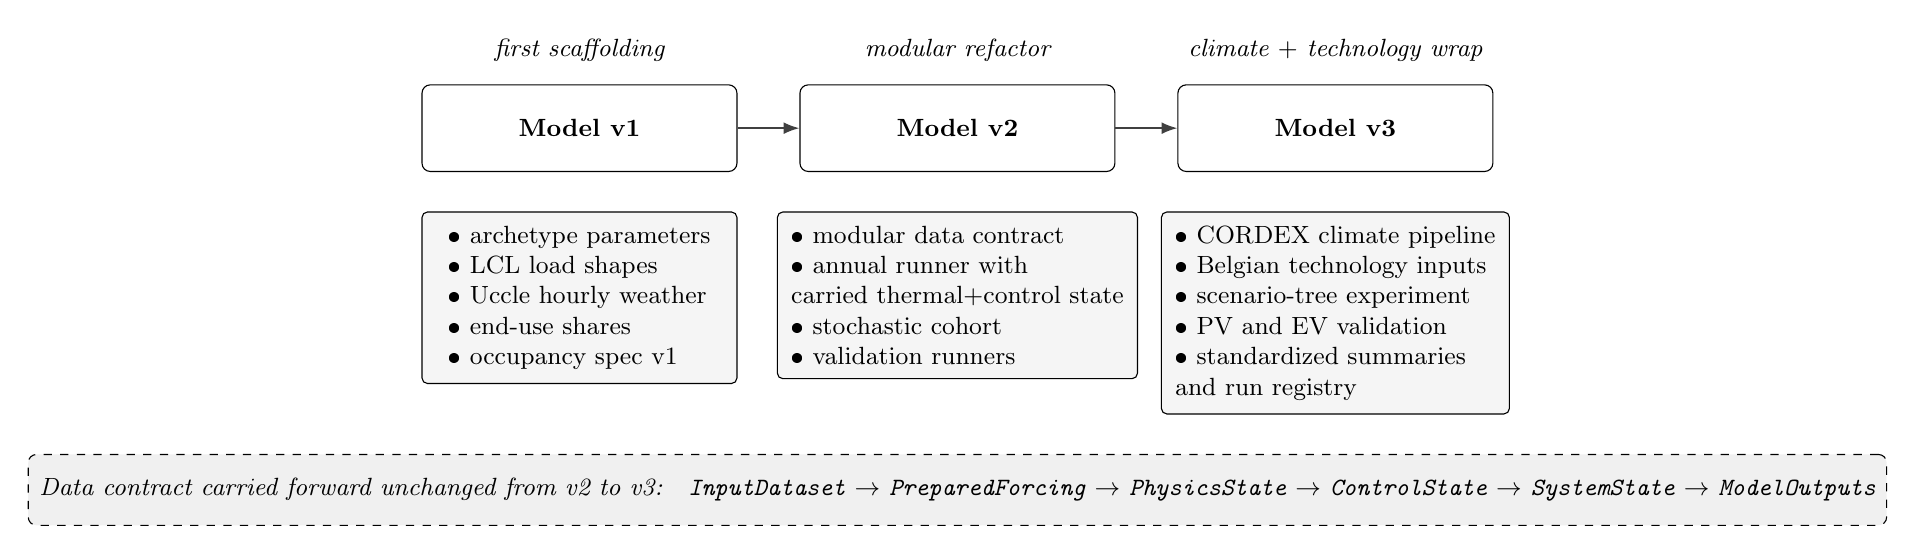
\begin{tikzpicture}[
      x=4.8cm, y=1.2cm,
      every node/.style={font=\small, align=center, inner sep=4pt},
      gen/.style={draw, rounded corners=3pt, minimum width=4cm,
                  minimum height=11mm, font=\small\bfseries},
      addbox/.style={draw, rounded corners=2pt, minimum width=4cm,
                     align=left, inner sep=5pt, fill=black!4,
                     font=\small},
      core/.style={draw, dashed, rounded corners=3pt,
                   minimum width=4cm, minimum height=9mm,
                   font=\small\itshape, fill=black!6},
      arrow/.style={-{Latex[length=2mm]}, semithick, draw=black!75},
  ]
    %% --- Generation headers ---
    \node[gen] (v1) at (0, 5) {Model v1};
    \node[gen] (v2) at (1, 5) {Model v2};
    \node[gen] (v3) at (2, 5) {Model v3};
    \draw[arrow] (v1) -- (v2);
    \draw[arrow] (v2) -- (v3);

    %% --- "What is added" boxes ---
    \node[addbox, below=5mm of v1] (a1) {
      \textbullet\ archetype parameters\\
      \textbullet\ LCL load shapes\\
      \textbullet\ Uccle hourly weather\\
      \textbullet\ end-use shares\\
      \textbullet\ occupancy spec v1};
    \node[addbox, below=5mm of v2] (a2) {
      \textbullet\ modular data contract\\
      \textbullet\ annual runner with\\carried thermal+control state\\
      \textbullet\ stochastic cohort\\
      \textbullet\ validation runners};
    \node[addbox, below=5mm of v3] (a3) {
      \textbullet\ CORDEX climate pipeline\\
      \textbullet\ Belgian technology inputs\\
      \textbullet\ scenario-tree experiment\\
      \textbullet\ PV and EV validation\\
      \textbullet\ standardized summaries\\and run registry};

    %% --- Preserved core banner ---
    \node[core, below=5mm of a3.south, xshift=-4.8cm,
          minimum width=13.6cm, anchor=north]
      (corebar) {Data contract carried forward unchanged from v2 to v3:\quad
      \texttt{InputDataset} $\to$ \texttt{PreparedForcing} $\to$
      \texttt{PhysicsState} $\to$ \texttt{ControlState} $\to$
      \texttt{SystemState} $\to$ \texttt{ModelOutputs}};

    %% --- Roles (above headers) ---
    \node[font=\small\itshape, above=1.5mm of v1] {first scaffolding};
    \node[font=\small\itshape, above=1.5mm of v2] {modular refactor};
    \node[font=\small\itshape, above=1.5mm of v3] {climate $+$ technology wrap};
  \end{tikzpicture}}
  \caption{Three-generation model development pathway.}
  \label{fig:model_hierarchy}
\end{figure}


\subsection{Model v1}
\label{sec:modelv1}

Model v1 established the first consistent set of Belgian residential inputs: archetypes, weather, load profiles, end-use shares, and an occupancy specification. Those inputs remain disclosed in \Cref{sec:model_inputs}; the v1 computation surface is not used for the thesis results.


\subsection{Model v2}
\label{sec:modelv2}

Model v2 introduced the typed data contract of \Cref{eq:dataContract}, the annual runner with carried indoor-temperature and thermostat state, the stochastic cohort wrapper, and the validation runners. These are inherited by v3.


\subsection{Model v3}
\label{sec:modelv3}

Model v3 is the version used to produce the thesis results. It keeps the v2 contract, annual runner, cohort engine, and validation runners, and adds the CORDEX climate pipeline, Belgian technology-case metadata, PV and EV layers, standardised scenario summaries, and the run registry.


%%% ----- %%%
\pagebreak
\section{Model Inputs}
\label{sec:model_inputs}
This section discloses the inputs that enter the model, where each input comes from, at what resolution, and in what role. Mechanical details---how an input is consumed by the physics, control, or systems layer---are deferred to \Cref{sec:modelling_framework}. \Cref{tab:inputs_overview} is the master index of inputs and points to the subsection that describes each group.

\begin{table}[ht]
  \centering
  \footnotesize
  \caption{Master index of model inputs. Role \texttt{input} feeds the simulation directly; \texttt{calibration} rescales a computed output to a target; \texttt{validation} is consumed only by the validation runners (\Cref{sec:validation}).}
  \label{tab:inputs_overview}
  \begin{tabular}{@{}p{0.27\linewidth} p{0.34\linewidth}
                    p{0.13\linewidth} p{0.13\linewidth}@{}}
    \toprule
    \textbf{Group} & \textbf{Active file(s)} &
    \textbf{Resolution} & \textbf{Role} \\
    \midrule
    Building \& archetype
      & \texttt{archetype\_parameters\_merged\_v3.csv}\newline
        \texttt{envelope\_archetypes\_v2.csv}\newline
        \texttt{internal\_gains\_archetypes\_v2.csv}\newline
        \texttt{airflow\_archetypes\_v2.csv}
      & --
      & input \\
    Occupancy \& behaviour
      & \texttt{occupancy\_model\_spec\_v1.yaml}
      & \SI{15}{min}
      & input \\
    Weather (historical)
      & \texttt{aws\_1hour\_Uccle.csv}
      & \SI{1}{h}
      & input \\
    Weather (PVGIS)
      & \texttt{Timeseries\_pvgisWEATHER\_*.csv}
      & \SI{1}{h}
      & input \\
    Climate projections
      & \texttt{weather\_\{window\}\_\{pathway\}\_*.csv} (CORDEX)
      & \SI{1}{d}
      & input \\
    Solar irradiance
      & \texttt{solardata\_*\_\{S,E,W,N\}\_2023\_2023.csv}\newline
        \texttt{Timeseries\{S,E,W,N\}\_*\_2005\_2023.csv}
      & \SI{1}{h}
      & input \\
    Macro end-use
      & \texttt{EU27\_BE\_household\_enduse\_2019.csv}
      & annual
      & calibration \\
    Belgian technology
      & \texttt{belgian\_technology\_inputs.yaml}
      & --
      & input \\
    Representative load
      & \texttt{LCL\_2013.csv}
      & \SI{30}{min}
      & input \\
    Smart-meter (DSO)
      & \texttt{P6269\_Open\_Data\_*.csv} (Fluvius)
      & \SI{15}{min}
      & validation \\
    Smart-meter (case study)
      & \texttt{house\_1,2,3-elec.csv} (KU\,Leuven)
      & \SI{1}{s}--\SI{1}{min}
      & validation \\
    PV reference
      & \texttt{ods032\_belgium\_pv\_*.csv} (Elia)
      & \SI{15}{min}
      & validation \\
    \bottomrule
  \end{tabular}
\end{table}


\subsection{Data Processing}
\label{sec:dataProcessing}
 
All inputs are funnelled through a single harmonisation layer that resamples each source to the canonical \SI{1}{h} timestep and reindexes it onto the configured simulation timeline. Harmonisation methods are set per input family in \texttt{config/thesis.yaml}: forward-fill for the weather record, mean aggregation for load profiles, internal gains and solar irradiance. Reconstruction methods, applied when a source has gaps, are forward-fill for weather and zero-fill for the other families; zero-fill is the conservative choice because it cannot fabricate end-use demand. \Cref{fig:data_pipeline} sketches the pipeline.

\begin{figure}[ht]
  \centering
  \begin{tikzpicture}[
      every node/.style={font=\scriptsize, align=center, inner sep=3pt},
      box/.style={draw, rounded corners=2pt, minimum height=8mm,
                  text width=2.8cm},
      smallbox/.style={draw, rounded corners=2pt, minimum height=8mm,
                  text width=2.5cm},
      groupbox/.style={draw, rounded corners=2pt, dashed, inner sep=5pt},
      arrow/.style={-{Latex[length=1.6mm]}, semithick, draw=black!75},
      sidearrow/.style={-{Latex[length=1.6mm]}, semithick, draw=black!60},
  ]

    % Row 1: time-series preparation
    \node[box] (tsrc) at (0,0)
      {Time-series sources\\weather, load profiles,\\internal gains, solar};

    \node[smallbox] (loaders) at (3.4,0)
      {Source loaders};

    \node[box] (harm) at (6.8,0)
      {Harmonisation\\to target timestep};

    \node[box] (recon) at (10.2,0)
      {Missing-data\\reconstruction};

    % Row 2: runtime forcing construction
    \node[smallbox] (input) at (0,-2.2)
      {\texttt{InputDataset}};

    \node[box] (adapter) at (3.4,-2.2)
      {Adapter layer\\semantic mapping};

    \node[smallbox] (forcing) at (6.8,-2.2)
      {\texttt{PreparedForcing}};

    \node[smallbox] (physics) at (10.2,-2.2)
      {Physics layer};

    % Row 3: metadata/config inputs
    \node[box] (meta) at (1.7,-4.3)
      {Parameter and metadata inputs,\\building archetypes,\\occupancy specs,\\technology configuration};

    % Group boxes
    \node[groupbox, fit=(tsrc)(loaders)(harm)(recon),
          label={[font=\scriptsize]above:Time-series preparation}] {};

    \node[groupbox, fit=(input)(adapter)(forcing),
          label={[font=\scriptsize]above:Runtime forcing construction}] {};

    % Main time-series arrows
    \draw[arrow] (tsrc.east) -- (loaders.west);
    \draw[arrow] (loaders.east) -- (harm.west);
    \draw[arrow] (harm.east) -- (recon.west);

    % Routed arrow from reconstructed time series to InputDataset.
    % It enters from the left to avoid crossing the dashed group boundary above InputDataset.
    \coordinate (reconDrop) at ($(recon.south)+(0,-0.75)$);
    \coordinate (leftRoute) at ($(input.west)+(-0.65,0)$);

    \draw[arrow]
      (recon.south) -- (reconDrop)
      -| (leftRoute)
      -- (input.west);

    % Runtime forcing path
    \draw[arrow] (input.east) -- (adapter.west);
    \draw[arrow] (adapter.east) -- (forcing.west);
    \draw[arrow] (forcing.east) -- (physics.west);

    % Metadata/config arrows
    \draw[sidearrow] (meta.north) to[out=90,in=-90] (input.south);
    \draw[sidearrow] (meta.north east) to[out=55,in=-90] (adapter.south);

  \end{tikzpicture}

  \caption{Runtime data preparation path for model v3.}
  \label{fig:data_pipeline}
\end{figure}

Time-series sources are loaded, harmonised to the target timestep, and reconstructed for missing values before being packaged into an \texttt{InputDataset}. The adapter layer then maps these processed sources, together with building, occupancy, and technology metadata, into the \texttt{PreparedForcing} object consumed by the physics layer.

\subsubsection*{Climate data}
For \hyperref[sec:scenarioTreeSystem]{scenario-tree} climate runs, the processed CORDEX forcing is consumed at its native daily cadence. The daily \texttt{tas} field is mapped to \texttt{T\_outdoor\_C}, and the daily \texttt{rsds} field is converted to \texttt{I\_solar\_W\_m2} during preprocessing and then used as a generic solar irradiance input in the forcing builder. The scenario adapter infers the timestep from the climate forcing file; for the processed CORDEX files this yields a daily timestep unless an explicit \texttt{target\_resolution\_seconds} override is supplied. Consequently, future-climate scenario outputs are interpreted at daily, seasonal, and annual horizons.

\subsubsection*{Quality control}
Quality control is enforced at three points. The AWS weather file carries the Royal Meteorological Institute of Belgium (RMI) per-row \texttt{qc\_flags}\footnote{Quality-control flags.}, preserved through the loader. The annual runner guards against incomplete weather years, requiring the reference year to span roughly \num{8760} hourly rows (\num{8784} on leap years) before \texttt{simulation.max\_steps} is applied, so truncated debug runs cannot pass as full-year results. The \hyperref[sec:scenarioTreeSystem]{scenario-tree} layer enforces the 2050 overlap policy so overlapping CORDEX source files are not double-counted across windows. Each input is also tagged with a data role (\texttt{input}, \texttt{calibration}, or \texttt{validation}), preventing calibration sources from being cited as independent validation evidence.


\subsection{Building Archetype}
\label{sec:input_building_archetype}
 
The active runtime archetype table is \texttt{archetype\_parameters\_merged\_v3.csv}. It contains \num{24} archetypes: four dwelling types (detached, semi-detached, terraced, apartment), each split into five construction-period \emph{as-is}\footnote{The as-is case represents the existing residential stock without additional retrofit measures or technology upgrades} bands plus one current-code \emph{renovated} package, for a total of $4 \times (5+1) = 24$ rows. Stock weights are drawn from the four-type R1--R4 Belgian dwelling shares and the type-specific construction-period shares published by Statbel \cite{Statbel2024Census}; envelope U-values for the as-is packages are taken from the Belgian TABULA building typology \cite{Loga2016TABULA,Cyx2011TABULABE}; and the renovated package applies current Flemish/Walloon EPB envelope levels: wall \SI{0.24}{W/m^2/K}, roof \SI{0.24}{W/m^2/K}, floor \SI{0.24}{W/m^2/K}, and window \SI{1.50}{W/m^2/K}.

\subsubsection*{Companion tables}
Three companion tables provide the parameters that are not part of the merged archetype row. The \texttt{envelope\_archetypes} file records the reconstructed envelope areas behind each archetype's $UA$ and $H$ values; \texttt{internal\_gains\_archetypes} records the heat-gain references used for occupant, appliance, lighting and cooking heat; and \texttt{airflow\_archetypes} records the infiltration and ventilation references.


\subsubsection*{Runtime selection}
Selection at runtime is configured through \texttt{building.archetype\_source.selection}; the canonical thesis setting is \texttt{stock\_weighted\_average} for the deterministic single-archetype run, and \texttt{uncertainty.physical.sample\_building\_archetype\_by\_stock\_weight} enables stock-weighted sampling for the cohort run.

\subsubsection*{Archetype sources}
\Cref{tab:archetype_sources} summarises the empirical basis of the archetype table. Known limitations are explicit: apartment age shares use a building-count age mix as a proxy for dwelling age, renovation prevalence is based on a regional EPC\,A/B proxy ($\sim\SI{15.99}{\percent}$ Belgian weighted high-performance share, flagged as \emph{implemented proxy}) rather than a direct type-by-age renovation matrix, and the TABULA U-values are archetype package values rather than measured field observations.
 
\begin{table}[ht]
  \centering
  \footnotesize
  \caption{Empirical basis of the building archetype table.}
  \label{tab:archetype_sources}
  \begin{tabular}{@{}p{0.34\linewidth} p{0.55\linewidth}@{}}
    \toprule
    \textbf{Dimension} & \textbf{Source} \\
    \midrule
    Dwelling-type shares (R1--R4)
      & Statbel 2024 census tables on the Belgian dwelling stock
        \cite{Statbel2024Census} \\
    Construction-period shares (per type)
      & Statbel 2024 type-specific period shares
        \cite{Statbel2024Census} \\
    As-is envelope U-values
      & Belgian TABULA construction-element values
        \cite{Loga2016TABULA,Cyx2011TABULABE} \\
    Renovated envelope package
      & Current Flemish/Walloon EPB requirements
        \cite{VEKAEnergyPerformance,SPWEnergyPerformance} \\
    Within-type renovation share
      & Belgian weighted EPC A/B high-performance proxy derived from
        regional EPC label distributions \cite{CLIMACT2024ResidentialRenovation,BISAMiniBru2025} \\
    \bottomrule
  \end{tabular}
\end{table}


% The building input layer is defined by the merged Model v2 archetype table, which segments the residential stock by dwelling type and renovation state. The table distinguishes detached, semi-detached, terraced, and apartment dwellings, each in as-is and renovated states. For each segment, it stores the parameters required by the thermal model: floor area, volume, heat-loss coefficient, effective thermal capacitance, comfort setpoints, infiltration and ventilation assumptions, glazing ratio, solar-gain factors, orientation shares, and default internal-gain parameters. This follows the general logic of residential building-stock typologies, where representative categories are used to describe heterogeneous dwelling populations while keeping the model tractable \cite{swan_modeling_2009,kavgicReviewBottomupBuilding2010,loga_tabula_nodate}.

% In the current implementation, the archetype table is the authoritative deterministic source for the base dwelling description. The runtime configuration selects a single archetype either explicitly by `archetype\_id` or, if configured differently, by the highest stock weight. The active thesis configuration selects an apartment as-is heat-pump archetype. The stock weights and dwelling-type labels are therefore present in the input table, but Model v2 does not yet sample dwelling categories across the full stock distribution. Instead, probabilistic household-level variation is introduced by perturbing the selected archetype. The cohort sampler applies multiplicative uncertainty factors to the heat-loss coefficient, thermal mass, infiltration rate, heating capacity, and coefficient of performance. Thus, archetypes should not be interpreted as exact dwellings; they provide stock-level central values around which the stochastic cohort is generated.

% The airflow parameters are also part of the archetype layer. Infiltration is represented through an air-change rate derived from an assumed airtightness level, while mechanical or natural ventilation is represented through base and occupied ventilation rates. Renovated archetypes are assigned lower default infiltration and mechanical-extract ventilation assumptions than as-is archetypes. These values are implementation assumptions documented in the merged archetype inputs, and are used as uncertainty-sensitive physical parameters rather than measured properties of individual dwellings. This treatment derived from the need to expose envelope and ventilation uncertainty in bottom-up residential models \cite{laverge2014airtightness}, particularly where airtightness data are incomplete or only available as population-level evidence.


\subsection{Occupancy \& Behaviour}
\label{sec:input_occupancy_behaviour}
Household occupancy is a three-state schedule, $\{\texttt{away},\texttt{awake},\texttt{sleep}\}$, at a \SI{15}{min} timestep conditioned on day-type (weekday/weekend). At each timestep, time-of-day rules set an absolute probability for one state and distribute the remaining mass via fallback weights. The spec also records state-specific \texttt{stickiness} fields as legacy Markov persistence parameters (\num{0.90} \texttt{away}, \num{0.80} \texttt{awake}, \num{0.97} \texttt{sleep}); these are stored for completeness but not consumed by the active forcing builder (\Cref{sec:occupancyStateModel}). The structure follows the multi-state occupancy formulation of \textcite{Richardson2010_DomesticHighRes}.

Behavioural variability across households is added at the cohort layer through the configuration's behaviour-uncertainty block. The active values for the canonical thesis run appear in \Cref{tab:behaviour_uncertainty}, with their interpretation as multiplicative log-normal perturbations given in \Cref{sec:modelling_framework}. The cohort sampler's household-size distribution is the Belgian private-household-size working distribution from Statbel \cite{Statbel2024Households}, truncated at seven persons.
 
\begin{table}[ht]
  \centering
  \footnotesize
  \caption{Behavioural uncertainty parameters consumed by the cohort
  sampler. Mechanistic interpretation is deferred to
  \Cref{sec:modelling_framework}.}
  \label{tab:behaviour_uncertainty}
  \begin{tabular}{@{}l l l@{}}
    \toprule
    \textbf{Parameter} & \textbf{Value} & \textbf{Affects} \\
    \midrule
    \texttt{occupancy\_sigma}           & 0.20 & occupancy intensity \\
    \texttt{dhw\_sigma}                 & 0.40 & DHW volume per household \\
    \texttt{dhw\_cohort\_scale}         & 3.217 & DHW magnitude calibration \\
    \texttt{appliance\_sigma}           & 0.50 & appliance baseline \\
    \texttt{dhw\_event\_lambda}         & 3.0 & DHW event rate \\
    \texttt{dhw\_event\_volume\_sigma}  & 0.40 & DHW event size \\
    \texttt{dhw\_start\_jitter\_hours}  & 0.75 & DHW event timing \\
    \texttt{appliance\_start\_jitter\_hours} & 1.0 & appliance event timing \\
    \texttt{high\_frequency\_sigma}     & 0.08 & sub-hourly variability \\
    \bottomrule
  \end{tabular}
\end{table}
Parameters denoted by $\sigma$ (\texttt{\_sigma}) control the dispersion of sampled household-level behavioural multipliers or event magnitudes, while $\lambda$ (\texttt{\_lambda}) controls the expected rate of stochastic DHW events. Larger $\sigma$ values increase inter-household or event-size variability, whereas a larger $\lambda$ increases the expected number of DHW draw events.

% The behavioural input layer describes how households use the dwelling over time. Model v2 separates this layer from the building physics because two dwellings with identical envelope and system parameters can produce different demand profiles when occupied, heated, ventilated, and used differently \cite{seryakOccupancyBehavioralAffects}. The model therefore treats occupancy, setpoints, domestic hot water, lighting, appliance events, and household class as behavioural drivers of demand rather than as fixed properties of the building.

% Occupancy is specified through a YAML state model with 15-minute slots, weekday/weekend conditioning, and three states: away, awake, and sleep. The implementation converts the time-of-day rules into weekday and weekend probability profiles. At each simulation step, the dominant state determines the schedule state used by the thermostat logic: occupied day, sleeping, or away. The same occupancy probabilities also determine expected occupants and occupant heat gains. Although the occupancy specification contains stickiness parameters, the current Model v2 forcing builder uses time-slot probability profiles and household-specific schedule perturbations rather than a full Markov transition simulation. This is a pragmatic simplification of the stochastic occupancy approaches commonly used in domestic energy-demand modelling \cite{Richardson2010_DomesticHighRes,widen_high-resolution_2010}.

% Behavioural heterogeneity is introduced in the cohort sampler. Each household receives a behavioural class, an occupancy intensity multiplier, schedule time shifts, state-bias factors, a setpoint shift, appliance and DHW intensity multipliers, and optional appliance ownership flags such as dryer and EV presence. These sampled parameters modify the deterministic input profiles before the annual simulation is run. Model v2 currently uses four household behaviour classes: low-flat, workday-absent, peak-heavy-family, and daytime-home. These classes are not directly estimated from the local validation data in the current repository, but they implement the modelling principle that household demand diversity is better represented by combining discrete behavioural regimes with continuous within-class variation \cite{Richardson2010_DomesticHighRes,widen_high-resolution_2010,Fischer2016_StochasticBottomUpHeatDHW}.

% Internal gains are assembled in the prepared-forcing layer from several components. Occupant heat gains are calculated from the occupancy probabilities and per-person gain assumptions in the archetype table. Appliance, lighting, and cooking heat gains are derived from the mapped electrical end-use profiles using fixed heat-recovery fractions. An explicit internal-gain time series can also be supplied, but the default configuration uses zero explicit gains, so the active internal-gain signal is mainly occupancy plus recovered end-use electricity. Lighting is additionally reshaped by occupancy and a daylight proxy derived from weather or facade irradiance. Domestic hot-water demand is generated as an occupancy-gated stochastic event process with shower, sink, and dishwashing events, while appliance and cooking demand include event-based starts for cooking, kettle, washing machine, dishwasher, dryer, and EV charging when present. These event-based elements are important because short-duration appliance and DHW events influence peak demand and household-to-household variability more strongly than annual energy totals alone \cite{Richardson2010_DomesticHighRes,widen_high-resolution_2010}.

% Ventilation behaviour is only partly behavioural in the current implementation. Base and occupied ventilation rates are physical archetype parameters, while the control layer can add an optional window-opening airflow term when the dwelling is occupied and indoor temperature exceeds the upper setpoint band. In the active configuration, this window-opening module is disabled. Therefore, ventilation and infiltration heat losses are active physical terms, but stochastic window-opening behaviour should not be overclaimed as a calibrated behavioural input in the current Model v2 version.


\subsection{Weather \& Climate}
\label{sec:weatherClimate}
 
Two weather sources feed the model and are kept strictly separate. The canonical historical-weather source is the RMI automatic-weather station record at Uccle \cite{RMI2024UccleAWS}. The active runtime column is \texttt{temp\_dry\_shelter\_avg} (dry-bulb shelter temperature, \SI{1}{h}), mapped to the model's \texttt{T\_outdoor\_C}. The canonical thesis run uses calendar year $2023$ because that year has the complete \SI{8760}{h} coverage required by the annual-runner guard.
 
The PVGIS hourly time series at the same point provides a long stationary historical sample ($2005$--$2023$) used by the climate-ensemble workflow \cite{Huld2012PVGIS}.

\subsubsection*{Future climate forcing}
Future climate forcing is supplied by EURO-CORDEX \cite{Jacob2014EuroCordex} regional projections, downloaded from the \href{https://apps.climate.copernicus.eu}{Copernicus Climate Data Store}. The configured chain is \texttt{cnrm\_cerfacs\_cm5} (GCM) $\times$ \texttt{cnrm\_aladin63} (RCM) $\times$ \texttt{r1i1p1}, with two daily-mean variables: \texttt{tas} (\SI{2}{m} air temperature) and \texttt{rsds} (surface solar radiation downwards). Spatial extraction is by nearest CORDEX grid point to Uccle/Brussels (target $50.85^{\circ}$N, $4.35^{\circ}$E; selected cell $50.798^{\circ}$N, $4.270^{\circ}$E). \Cref{tab:climate_inventory} lists the processed files actually present under \texttt{inputs/climate/processed/}.
 
\begin{table}[ht]
  \centering
  \footnotesize
  \caption{Processed CORDEX forcing files}
  \label{tab:climate_inventory}
  \begin{tabular}{@{}l l l@{}}
    \toprule
    \textbf{Window} & \textbf{Canonical span} & \textbf{Pathways} \\
    \midrule
    \texttt{baseline}     & $1981$--$2005$ & historical \\
    \texttt{near\_future} & $2030$--$2049$ & rcp\_2\_6, rcp\_4\_5, rcp\_8\_5 \\
    \texttt{mid\_century} & $2050$--$2070$ & rcp\_2\_6, rcp\_4\_5, rcp\_8\_5 \\
    \texttt{long\_term}   & $2080$--$2100$ & rcp\_2\_6, rcp\_4\_5, rcp\_8\_5 \\
    \bottomrule
  \end{tabular}
\end{table}
 
Orientation-resolved solar irradiance is provided by \href{https://joint-research-centre.ec.europa.eu/photovoltaic-geographical-information-system-pvgis_en}{PVGIS-SARAH3} \cite{Pfeifroth2018SARAH} at the same Uccle/Brussels coordinates: hourly facade irradiance for South, East, West, and North orientations at $90^{\circ}$ tilt, both for the canonical year $2023$ and for the climate sample $2005$--$2023$. Columns are global beam, diffuse, and reflected—\texttt{Gb(i)}, \texttt{Gd(i)} and \texttt{Gr(i)} respectively—plane-of-array irradiance, sun elevation, $\SI{2}{m}$ air temperature, and $\SI{10}{m}$ wind speed.

\begin{figure}[ht]
  \centering
  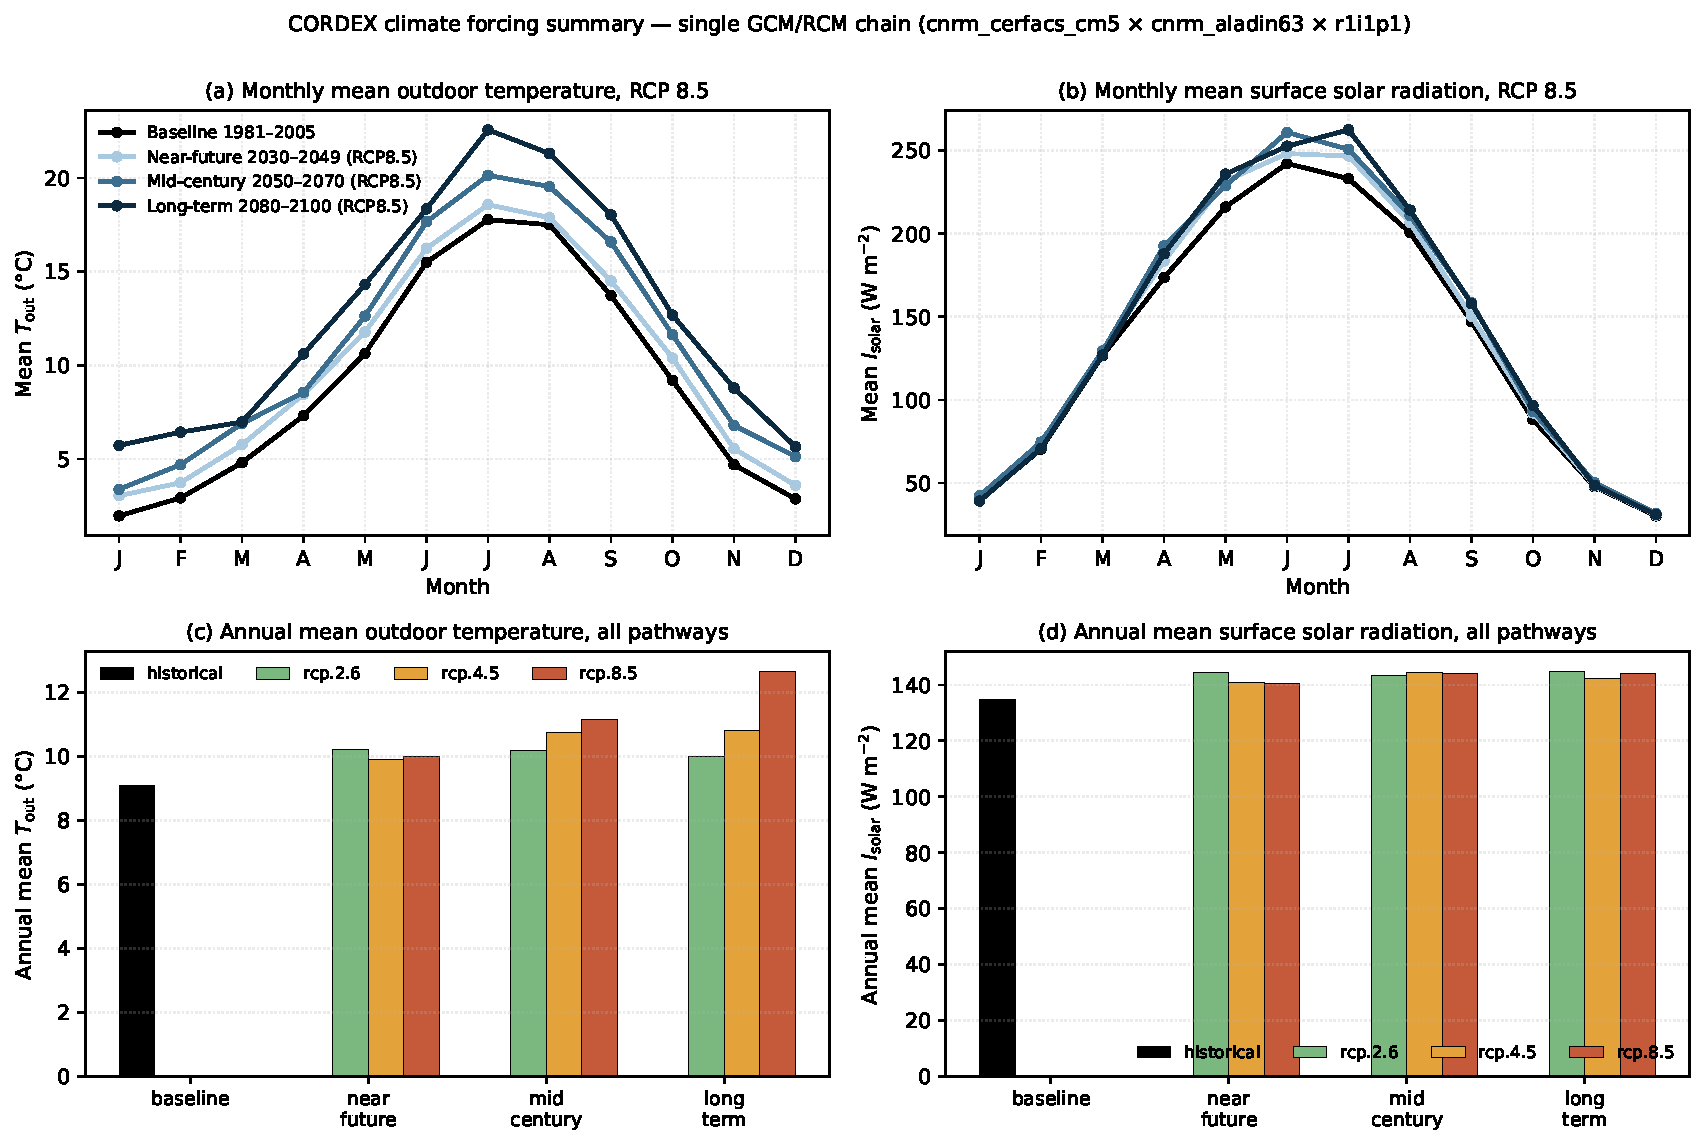
\includegraphics[width=\textwidth]{figures/climate_forcing_summary.pdf}
  \caption{CORDEX climate forcing summary, single GCM/RCM chain.}
  \label{fig:climate_forcing_summary}
\end{figure}

Panels (a) and (b) of \Cref{fig:climate_forcing_summary} show the monthly climatology of outdoor temperature and surface solar radiation for the baseline window (black) and the three future windows under RCP\,8.5 (blue shades, darker $=$ further future); the temperature signal concentrates in the warm half of the year.
\newline Panels (c) and (d) give annual means across the four windows and the historical, RCP\,2.6, RCP\,4.5, and RCP\,8.5 pathways: annual mean $T_{\text{out}}$ rises from $\sim\SI{9.1}{\celsius}$ at baseline to $\sim\SI{12.6}{\celsius}$ in the long-term RCP\,8.5 cell, while annual mean $I_{\text{solar}}$ stays within $\sim\SI{135}{\watt\per\square\meter}$ to $\sim\SI{145}{\watt\per\square\meter}$ across all futures.


\subsection{Macro \& Benchmark}
\label{sec:macro_benchmark}

Two configuration files anchor the model to Belgian macro evidence: the Eurostat \texttt{nrg\_d\_hhq} end-use shares for the Belgian and EU-27 residential sectors \cite{eurostat_disaggregated_nodate}, together with macro context from \texttt{ten00124}, \texttt{ten00123} and \texttt{ten00125} \cite{EurostatTen00124,EurostatTen00125}. The relevant Belgian shares are reproduced in \Cref{tab:macro_benchmark}.

\begin{table}[ht]
  \centering
  \footnotesize
  \caption{Belgian residential end-use shares and macro context.}
  \label{tab:macro_benchmark}
  \begin{tabular}{@{}l r l@{}}
    \toprule
    \textbf{Quantity} & \textbf{Value (\%)} & \textbf{Source} \\
    \midrule
    Space heating share        & 73.01 & \texttt{nrg\_d\_hhq} \\
    Water heating share        & 12.00 & \texttt{nrg\_d\_hhq} \\
    Cooking share              &  1.64 & \texttt{nrg\_d\_hhq} \\
    Space cooling share        &  0.07 & \texttt{nrg\_d\_hhq} \\
    Residual (appl.+light.+other) & 13.29 & \texttt{nrg\_d\_hhq} \\
    \midrule
    Residential share of final energy (BE, 2022)  & 24.0 & \texttt{ten00124} \\
    Electricity share of final energy (BE, 2022)  & 21.7 & \texttt{ten00123} \\
    Household electricity share (BE, 2022)        & 19.1 & \texttt{ten00125} \\
    \bottomrule
  \end{tabular}
\end{table}

\subsubsection*{Energy carriers \& technology}
The \texttt{belgian\_technology\_inputs.yaml} file records the Belgian carrier and technology metadata used by the technology cases of the \hyperref[sec:scenarioTreeSystem]{scenario tree}. It is compiled from the sources listed in \Cref{tab:belgian_tech_sources} and contains for each technology: a reference year, a low/base/high range and a suitability note. The headline carrier shares used as the canonical baseline are gas $0.637$, heating oil $0.211$, with the remainder split between electric, biomass, district heat and other, consistent with the \textcite{KBSFrb2024} and the JRC \cite{JRC2022HeatPumpBelgium}.

\begin{table}[ht]
  \centering
  \footnotesize
  \caption{Belgian technology evidence sources.}
  \label{tab:belgian_tech_sources}
  \begin{tabular}{@{}p{0.32\linewidth} p{0.20\linewidth} p{0.40\linewidth}@{}}
    \toprule
    \textbf{Source} & \textbf{Reference year} & \textbf{Used for} \\
    \midrule
    KBS-Frb Energy-Poverty Barometer \cite{KBSFrb2024}
      & $2022$ & main-heating carrier shares \\
    JRC Country Fiche: Belgian heat-pump market \cite{JRC2022HeatPumpBelgium}
      & $2022$ & gas-boiler / heat-pump installed stock \\
    RAP Country Report Belgium \cite{RAP2020BelgiumReport}
      & $2020$ & DHW carrier mix; district-heating context \\
    KU Leuven HP performance working paper \cite{KULeuvenHP2015}
      & $2015$ & Belgian heat-pump SPF ranges \\
    IEA PVPS Belgium 2024 \cite{IEAPVPS2024Belgium}
      & $2024$ & national cumulative PV capacity \\
    BRUGEL Annual Report \cite{Brugel2024Annual}
      & $2024$ & Brussels regional PV anchor \\
    Statbel EV stock \cite{Statbel2025EV}
      & $2025$ & BEV stock; registration split \\
    Statbel vehicles per household \cite{Statbel2024VehiclesHousehold}
      & $2024$ & car-ownership conditioning \\
    Federal carbon \& energy taxation landscape \cite{Climat2025Taxation}
      & $2025$ & EV annual distance; electricity intensity \\
    CRM Monitoring Report \cite{CRM2025Monitoring}
      & $2024$ & Flemish home-battery stock \\
    \bottomrule
  \end{tabular}
\end{table}

\subsubsection*{Energy shares}
The annual calibration baseline itself sits in \texttt{config/thesis.yaml}: annual electricity \SI{3500}{kWh} (\SIrange{3000}{3900}{kWh}), annual space heating \SI{12000}{kWh} (\SIrange{12000}{16000}{kWh}), and annual domestic hot water \SI{3000}{kWh} (\SIrange{2500}{3300}{kWh}). Electric DHW and space-heating shares are kept modest because thermal services are primarily represented through useful heat and carrier conversion rather than as dominant baseline electric loads. This decision is mainly driven by the fact that Belgian residential heating is gas-dominated: the main-heating carrier shares of $\sim$\SI{64}{\percent} gas and $\sim$\SI{21}{\percent} heating oil \cite{KBSFrb2024,JRC2022HeatPumpBelgium} leave only a small electric-heating minority, so the share of total electricity that goes to space heating in a representative dwelling is correspondingly small even though the share of total final energy going to space heating is large \cite{eurostat_disaggregated_nodate}.


\subsection{Smart Meter Data}
\label{sec:smartMeterData}

The smart-meter inputs serve various purposes and are kept
strictly separate.
 
\subsubsection*{Representative shape input} 
The Low Carbon London (LCL) dataset \cite{LowCarbonLondon2014} includes the load profiles of ${\sim}5500$ London households at \SI{30}{min} resolution, is stored as input-csv file, and is used inside the loader as a representative electrical load \emph{shape} that is subsequently rescaled to the Belgian annual baseline. LCL is deliberately treated as an internal shape source and is not used as thesis-facing aggregate validation evidence, because validating against the same family of data that supplies the input shape would not constitute an independent check.
 
\subsubsection*{Belgian aggregate validation} 
The Flemish DSO Fluvius publishes representative residential profiles disaggregated by heat-pump, EV and PV indicators \cite{Fluvius2024OpenData}. Eight combinations are stored under the fluvius-input file: \texttt{geen\_ZP}, \texttt{enkel\_ZP}, \texttt{WP\_geen\_ZP}, \texttt{WP\_met\_ZP}, \texttt{EV\_geen\_ZP}, \texttt{EV\_met\_ZP}, \texttt{WP\_EV\_geen\_ZP}, and \texttt{WP\_EV\_met\_ZP}\footnote{WP means ``warmtepomp''; meaning heat pump. ZP means ``zonnepanelen''; meaning PV panels.}. The schema is per connection-point (\texttt{EAN\_ID}\footnote{An EAN (European Article Number) is the unique 18-digit identifier of a physical electricity or gas connection point in the Belgian and Dutch markets, assigned by the distribution system operator (DSO). Each meter, and therefore each household, has one.}) \SI{15}{min} rows with consumption and injection plus equipment indicators. Fluvius profiles are the aggregate-validation source in \Cref{sec:validation}.
 
\subsubsection*{Belgian high-frequency case study} 
The KU\,Leuven three-house dataset \cite{KULeuven3House} provides high-frequency electrical (and partial gas) measurements for three Belgian dwellings, summarised in \Cref{tab:kul_houses}. The dataset is used only as a high-frequency event-realism check, validating ramps, spikes, daily peaks, etc. (\Cref{sec:validation}).

\begin{table}[ht]
  \centering
  \footnotesize
  \caption{KU\,Leuven three-house high-frequency dataset.}
  \label{tab:kul_houses}
  \begin{tabular}{@{}l l l l l@{}}
    \toprule
    \textbf{House} & \textbf{Type} & \textbf{EPC} &
      \textbf{Equipment} & \textbf{2023 coverage} \\
    \midrule
    1 & detached
      & A (\SI{39}{kWh/m^2})
      & PV, $\text{HP}_\text{geo}$, EV
      & six segments \\
    2 & apartment
      & B (\SI{162}{kWh/m^2})
      & none
      & three segments \\
    3 & attached
      & B (\SI{135}{kWh/m^2})
      & PV
      & one segment \\
    \bottomrule
  \end{tabular}
\end{table}

\subsubsection*{Belgian PV reference} 
The aggregate Belgian transmission-PV generation series published by Elia \cite{Elia2024PVODS032} is stored in the \texttt{ods032.csv} file at \SI{15}{min} resolution, with columns \texttt{measured}, \texttt{monitoredcapacity} and \texttt{loadfactor}. It is used as the country-level PV anchor for the PV triangle validation (\Cref{sec:validation}).


% Macro-level inputs are used as calibration anchors and plausibility context. The configuration contains annual baseline values for total household electricity, space heating, and domestic hot water, together with an electricity end-use split. During the annual simulation, Model v2 rescales modelled electricity end uses to the configured annual electricity targets. This means that the macro inputs constrain annual energy levels, while the hourly and sub-hourly temporal structure remains determined by the load-shape source, stochastic events, occupancy, thermal physics, and weather forcing.

% The repository also loads a Eurostat-derived household end-use table for Belgium and the EU-27 \cite{eurostat_disaggregated_nodate}. In the active data loader, the Belgian water-heating, cooking, and residual lighting/appliance shares are used to disaggregate the representative Low Carbon London aggregate electricity profile into appliances, lighting, cooking, and DHW components. The lighting share is further split from the combined appliance-lighting bucket using a configured fraction.

% For aggregate validation, the repository includes a Fluvius external validation path. The Fluvius loader reads quarter-hourly representative electricity profiles, converts interval energy to average power, groups profiles by technology category such as base, EV, heat pump, and combined EV/heat-pump, and constructs a weighted representative profile. The validation runner then scales both model and Fluvius profiles by the configured household count and compares absolute aggregate demand metrics. This is best interpreted as an aggregate-profile plausibility check rather than direct feeder validation, because the Fluvius inputs are representative profile data rather than a measured feeder serving the simulated households.

% \subsection{Smart-Meter Data}

% The model uses smart-meter data in two distinct ways. First, the active runtime load-shape source is the refactored Low Carbon London 2013 dataset. The loader reads the half-hourly household columns, computes the mean profile across meters, interprets the values as kWh per interval, converts them to average watts, and then splits the aggregate profile into end-use components using the Eurostat-derived shares. This profile is therefore an input shape source rather than an independent validation target. It should be noted that Low Carbon London should not be used as thesis-facing validation evidence in this configuration, because it already influences the modelled load shape \cite{tindemans2023lclRefactored}.

% Second, independent smart-meter or metered profile data are used for validation diagnostics. The KU Leuven validation path loads the PREMISES smart-meter measurements for three Belgian households \cite{palaciosGarcia2024premises}, detects whether each file contains direct power or cumulative energy, converts the signal to kW where needed, aggregates it to 15-minute mean power, maps the timestamps onto the model reference year, and compares the resulting profiles with model output. The validation metrics focus on high-frequency realism: daily maxima, spike counts, ramp rates, variance, skewness, kurtosis, and short visual segments. This dataset is therefore used as a case-study benchmark for event and ramp behaviour., not as a statistical calibration sample for the whole Belgian residential stock.

% The distinction between calibration and validation data is important. Low Carbon London contributes to the simulated temporal shape and is therefore part of the model input chain. Eurostat contributes annual and end-use calibration information. Fluvius and KU Leuven provide external plausibility checks at different aggregation levels: Fluvius for representative aggregate profiles and KU Leuven for high-frequency household event structure. This separation prevents the same data source from being treated simultaneously as an input and as independent evidence of model validity.


% \subsection{Preprocessing}
% %%% canonical timestamps
% %%% timezone handling
% %%% missing-data policy
% %%% reproducibility and audit trail



%%% --- %%%
\pagebreak
\section{Modelling Framework}
\label{sec:modelling_framework}

This subsection deconstructs the model architecture: how the inputs disclosed in \Cref{sec:model_inputs} are turned into per-timestep, per-household, per-scenario outputs. 
\newline The subsections below treat the layers in the order they execute (\hyperref[sec:archetypeConstruction]{archetype} $\to$ \hyperref[sec:occupancyStateModel]{occupancy} $\to$ \hyperref[sec:deterministicBaselineDemandModel]{deterministic baseline} $\to$ \hyperref[sec:stochasticScenarioGeneration]{stochastic cohort}), then describe the two outer wraps that vary the exogenous inputs (\hyperref[sec:climateScenariosFramework]{climate scenarios}, \hyperref[sec:climateUncertainty]{climate uncertainty}), and close with the output ledger.


\subsection{Archetype Construction}
\label{sec:archetypeConstruction}

The model represents the dwelling as one lumped thermal zone, fully described by a small parameter vector. \Cref{tab:archetype_params} lists the parameters that enter the physics layer. They are sourced from the \num{24}-row archetype table introduced in \Cref{sec:input_building_archetype} and from the companion envelope, internal-gain and airflow reference tables.

% \begin{table}[ht]
%   \centering
%   \footnotesize
%   \caption{Per-archetype parameter vector consumed by the physics
%   layer. Symbols match the variable names used in the implementation
%   (\texttt{src/model\_v3/interfaces.py}).}
%   \label{tab:archetype_params}
%   \begin{tabular}{@{}l l l@{}}
%     \toprule
%     \textbf{Symbol} & \textbf{Meaning} & \textbf{Source} \\
%     \midrule
%     $\text{stock\_weight}$
%       & weight in stock-weighted sampling
%       & Statbel dwelling stock \cite{Statbel2024Census} \\
%     $UA$ (\texttt{heat\_loss\_coefficient\_W\_per\_C})
%       & envelope conductance
%       & Belgian TABULA \cite{Cyx2011TABULABE} + reconstructed areas \\
%     $C$ (\texttt{thermal\_mass\_Wh\_per\_C}, \texttt{C\_J\_per\_K})
%       & effective thermal capacitance
%       & archetype default \\
%     $V$ (\texttt{volume\_m3})
%       & dwelling air volume
%       & reconstructed envelope geometry \\
%     $\text{ACH}_{\text{inf}}, \text{ACH}_{\text{vent,base/occ}}$
%       & infiltration and ventilation air-change rates
%       & Belgian airtightness anchors
%         ($\text{ACH}_{50}$ as-is $6.3$, renovated $2.5$)
%         \cite{Cyx2011TABULABE,Hens2007Airtightness}; ventilation
%         flow defaults from EN\,16798-1
%         \cite{EN16798_1_2019} \\
%     \texttt{ventilation\_type}, $\eta_{\text{HRV}}$
%       & ventilation regime, heat-recovery effectiveness
%       & EPB ventilation classes
%         \cite{VEKAEnergyPerformance,SPWEnergyPerformance};
%         $\eta_{\text{HRV}}$ from EN\,308 product range
%         \cite{EN308_HRV} \\
%     $Q_{\text{occ}}, Q_{\text{app}}, Q_{\text{light}}, Q_{\text{cook}}$
%       & internal gain references
%       & per-person sensible gains from ISO 13790 / EN\,16798-1
%         \cite{ISO13790_2008,EN16798_1_2019}; floor area from TABULA
%         type means \cite{Cyx2011TABULABE} \\
%     $T_{\text{set}}, T_{\text{min}}, T_{\text{max}}$
%       & comfort setpoint and band
%       & archetype comfort defaults \\
%     $Q_{\text{heat,max}}$, \texttt{heating\_cop}, \texttt{dhw\_cop}
%       & heating capacity and conversion COP
%       & technology case + heat-pump performance model \\
%     \bottomrule
%   \end{tabular}
% \end{table}

\begin{table}[ht]
  \centering
  \footnotesize
  \caption{Per-archetype parameter vector consumed by the physics
  layer. Symbols match the variable names used in the implementation.}
  \label{tab:archetype_params}
  \begin{tabular}{@{}p{0.27\linewidth} p{0.27\linewidth}
                   p{0.40\linewidth}@{}}
    \toprule
    \textbf{Symbol} & \textbf{Meaning} & \textbf{Source} \\
    \midrule
    $\text{stock\_weight}$
      & weight in stock-weighted sampling
      & Statbel dwelling stock \cite{Statbel2024Census} \\
    $UA$
      & envelope conductance
      & Belgian TABULA \cite{Cyx2011TABULABE} $+$ reconstructed areas \\
    $C$
      & effective thermal capacitance
      & archetype default \\
    $V$
      & dwelling air volume
      & reconstructed envelope geometry \\
    $\text{ACH}_{\text{inf}}, \text{ACH}_{\text{vent,base/occ}}$
      & infiltration and ventilation air-change rates
      & Belgian airtightness anchors
        ($\text{ACH}_{50}$ as-is $6.3$, renovated $2.5$)
        \cite{Cyx2011TABULABE,Hens2007Airtightness};
        ventilation defaults from EN\,16798-1
        \cite{EN16798_1_2019} \\
    \texttt{ventilation\_type}, $\eta_{\text{HRV}}$
      & ventilation regime, heat-recovery effectiveness
      & EPB classes
        \cite{VEKAEnergyPerformance,SPWEnergyPerformance};
        $\eta_{\text{HRV}}$ from EN\,308 \cite{EN308_HRV} \\
    $Q_{\text{occ}}, Q_{\text{app}}, Q_{\text{light}}, Q_{\text{cook}}$
      & internal gain references
      & per-person gains from ISO\,13790 / EN\,16798-1
        \cite{ISO13790_2008,EN16798_1_2019}; floor area from TABULA
        \cite{Cyx2011TABULABE} \\
    $T_{\text{set}}, T_{\text{min}}, T_{\text{max}}$
      & comfort setpoint and band
      & archetype comfort defaults \\
    \texttt{heating\_cop}, \texttt{dhw\_cop}
      & heating capacity and conversion COP
      & technology case $+$ heat-pump performance model \\
    \bottomrule
  \end{tabular}
\end{table}

\subsubsection*{Assignment modes}
Assignment from the building stock to one archetype follows three modes. The deterministic single-archetype mode builds one representative dwelling whose parameters are the stock-weighted average over the 24 rows. The deterministic single-row mode picks the most prevalent archetype. The stochastic mode draws one archetype per household with probability equal to its stock weight, so that the cohort population reproduces the Belgian dwelling-type and construction-period distribution in expectation.

\subsubsection*{Physical heterogeneity}
Independent physical heterogeneity is added on top of the archetype draw. The cohort sampler multiplies $UA$ by a normal scale factor ($\sigma_{UA}=0.25$), the thermal mass by a normal factor ($\sigma_{C}=0.20$), the infiltration rate by a log-normal factor ($\sigma_{\text{inf}}=0.40$), and the heating COP by a normal factor ($\sigma_{\text{COP}}=0.10$), each clipped to a physically meaningful range\footnote{Concrete bounds are encoded in the \texttt{sampler.py} file; e.g.\ the $UA$ scale is clipped to $[0.4, 2.0]$, infiltration to $[0.3, 3.5]$, COP to $[0.5, 1.5]$.}. This separation between archetype and per-household perturbation is what gives the cohort both Belgian-stock realism and within-stock variability.

\subsubsection*{Heating and emitter systems}
Each archetype is also paired with a heating-system class and an emitter type. Heating-technology probabilities can come from two sources: explicit \emph{technology-case} probabilities encoded by the scenario tree, and the Belgian carrier stock baseline from the Belgian technology inputs YAML file. The emitter family (underfloor, low-temperature radiator, standard radiator, high-temperature radiator, fan coil) is drawn from a configurable distribution and is the input to the weather-dependent heat-pump COP model (\Cref{sec:deterministicBaselineDemandModel}).


\subsection{Occupancy State Model}
\label{sec:occupancyStateModel}

Occupancy is modelled as a three-state homogeneous-in-day-type schedule, $\{\texttt{away},\texttt{awake},\texttt{sleep}\}$, at a \SI{15}{min} timestep, conditioned on weekday vs weekend. For each timestep, two sources combine to produce the state distribution. First, the configured time-of-day rules prescribe an absolute probability $p_{\text{rule}}(s)$ for some state $s$ (e.g.\ $P(\text{sleep} \mid 23\!:\!00\text{--}07\!:\!00, \text{weekday}) = 0.85$). Second, any remaining probability mass is allocated according to fallback weights for the day-type. The resulting three-state schedule follows the structure of multi-state occupancy models such as \textcite{Richardson2010_DomesticHighRes}, but transition persistence is represented indirectly through broad time-of-day windows and cohort-level schedule perturbations rather than through an explicit Markov stickiness matrix\footnote{The spec also records state-specific \texttt{stickiness} fields, intended as legacy Markov persistence parameters (higher for \texttt{sleep} than for \texttt{awake} on the plausible reasoning that sleep dwell times are longer than evening activity dwell times). They are not consumed by the active \texttt{forcing\_builder.py} loader and are therefore not used in the results of \Cref{ch:results}.}.

\subsubsection*{Household variability}
Household-specific variability is added at the cohort layer. Each household draws an occupancy-intensity scale, a $\pm\SI{2}{h}$ time-shift on the schedule, a state-duration log-normal scale, and a triple of log-normal state biases. The household's behavioural class (\texttt{low\_flat}, \texttt{workday\_absent}, \texttt{peak\_heavy\_family}, \texttt{daytime\_home}) further modulates the occupancy scaling factor, the appliance event intensity, and the peak sensitivity. Household size is drawn from a Belgian working distribution (1--7 persons) and is used to scale appliance and DHW activity through a sub-linear exponent (the \texttt{household\_size\_activity\_scale} factor is $(n_{\text{occ}}/n_{\text{ref}})^{0.65}$ with $n_{\text{ref}}=2$, clipped to $[0.55, 2.25]$); the choice of a sub-linear scaling reflects shared-load saturation effects observed in metered household samples \cite{Wilke2013StochasticOccupancy}. \Cref{tab:household_size_dist} shows the working Belgian distribution recorded in \texttt{config/thesis.yaml}. The rounded probabilities sum to $0.995$ and are renormalised at draw time. The values are anchored to Statbel household statistics for Belgium \cite{Statbel2024Households} and cross-checked against OECD family-composition data \cite{OECDFamilyDatabase}. Notably, the share of 1-person households dominates in Belgium. A residual cluster of 0.03 was used for 5+ persons per household (PPH).

\begin{table}[ht]
  \centering
  \footnotesize
  \caption{Household-size distribution used by the cohort sampler.}
  \label{tab:household_size_dist}
  \begin{tabular}{@{}c c@{}}
    \toprule
    \textbf{PPH} & \textbf{Probability}\\
    \midrule
    1 & 0.360 \\
    2 & 0.310 \\
    3 & 0.145 \\
    4 & 0.110 \\
    5 & 0.040 \\
    6 & 0.020 \\
    7 & 0.010 \\
    \bottomrule
  \end{tabular}
\end{table}

The occupancy state is the coupling point between behaviour and physics. It drives the active ventilation regime, the internal-gain magnitudes, the appliance and DHW event-generation rates, and the active setpoint via the schedule state (\texttt{occupied\_day}, \texttt{evening}, \texttt{sleep}).

\subsubsection*{Occupancy state coupling}
\Cref{fig:occupancy_coupling} sketches how the sampled occupancy state is consumed by four downstream layers in each timestep: ventilation regime, internal gains, appliance/DHW event rates, and active thermostat setpoint. This coupling allows behaviour to affect both electrical end-use timing and thermal demand without merging the behaviour, physics, and control code paths.

\begin{figure}[ht]
  \centering
  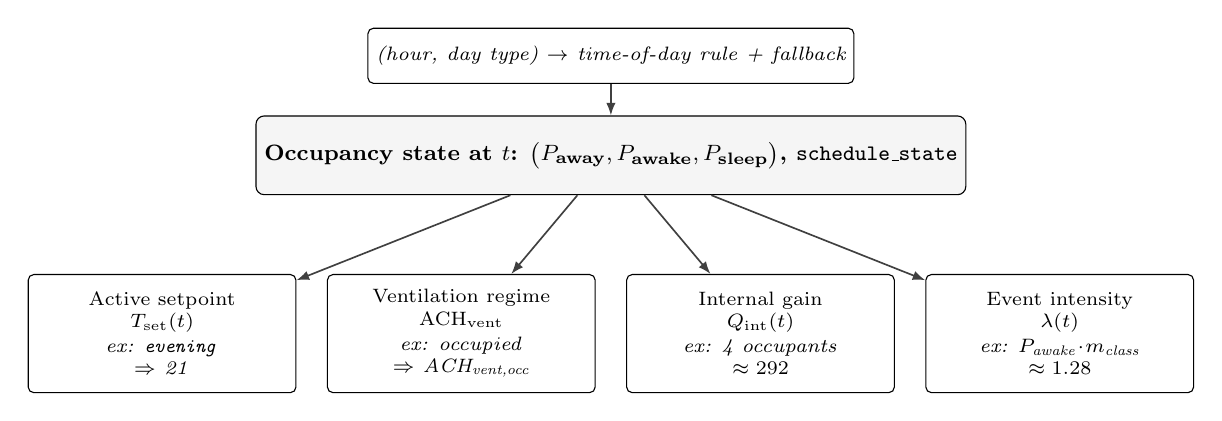
\begin{tikzpicture}[
      every node/.style={font=\scriptsize, align=center, inner sep=3pt},
      hub/.style={draw, rounded corners=3pt, fill=black!4,
                  minimum width=6.0cm, minimum height=10mm,
                  font=\footnotesize\bfseries},
      input/.style={draw, rounded corners=2pt,
                    minimum width=6.0cm, minimum height=7mm,
                    font=\scriptsize\itshape},
      outblock/.style={draw, rounded corners=2pt,
                       minimum width=3.4cm, minimum height=15mm},
      arrow/.style={-{Latex[length=1.6mm]}, semithick, draw=black!75},
      node distance=4mm and 4mm,
  ]
    \node[input] (rules)
      {(hour, day type) $\to$ time-of-day rule + fallback};
    \node[hub, below=of rules] (state)
      {Occupancy state at $t$:
       $\bigl(P_{\text{away}},P_{\text{awake}},P_{\text{sleep}}\bigr)$,
       \texttt{schedule\_state}};
    \draw[arrow] (rules) -- (state);
 
    \node[outblock, below=10mm of state, xshift=-5.7cm] (set)
      {Active setpoint\\$T_{\text{set}}(t)$\\[1pt]
       \emph{ex: \texttt{evening}}\\\emph{$\Rightarrow$ \SI{21}{\celsius}}};
    \node[outblock, below=10mm of state, xshift=-1.9cm] (vent)
      {Ventilation regime\\$\text{ACH}_{\text{vent}}$\\[1pt]
       \emph{ex: occupied}\\\emph{$\Rightarrow$ $\text{ACH}_{\text{vent,occ}}$}};
    \node[outblock, below=10mm of state, xshift= 1.9cm] (gain)
      {Internal gain\\$Q_{\text{int}}(t)$\\[1pt]
       \emph{ex: 4 occupants}\\\emph{$\approx\SI{292}{\watt}$}};
    \node[outblock, below=10mm of state, xshift= 5.7cm] (evt)
      {Event intensity\\$\lambda(t)$\\[1pt]
       \emph{ex: $P_{\text{awake}}\!\cdot\!m_{\text{class}}$}\\
       \emph{$\approx 1.28$}};
 
    \draw[arrow] (state) -- (set);
    \draw[arrow] (state) -- (vent);
    \draw[arrow] (state) -- (gain);
    \draw[arrow] (state) -- (evt);
  \end{tikzpicture}
  \caption{Occupancy state as the coupling point between behaviour
  and physics.}
  \label{fig:occupancy_coupling}
\end{figure}



\subsection{Deterministic Baseline Demand Model}
\label{sec:deterministicBaselineDemandModel}

The deterministic baseline is one dwelling running through the configured year hour by hour, with the indoor temperature and thermostat state carried forward across timesteps. It is implemented by \texttt{simulation/annual\_runner.py} as a sequence of four layers per timestep.

\subsubsection*{Physics layer}
The lumped-zone thermal balance integrates indoor temperature $T_{\text{in}}$ over the timestep $\Delta t$ with an adaptive explicit substep:
\begin{equation}
  C\,\frac{\mathrm{d}T_{\text{in}}}{\mathrm{d}t}
  = \underbrace{(UA + H_{\text{ve}})\,(T_{\text{out}} - T_{\text{in}})}_{\text{losses}}
  + \underbrace{Q_{\text{int}} + Q_{\text{sol}}}_{\text{gains}}
  + Q_{\text{heat}},
  \label{eq:thermal_balance}
\end{equation} where $H_{\text{ve}} = \rho\, c_p\, \dot V_{\text{eff}}$ is the ventilation-and-infiltration heat-transfer coefficient, $\dot V_{\text{eff}} = \dot V_{\text{inf}} + (1 - \eta_{\text{HRV}})\, \dot V_{\text{vent}}$ for a balanced system with heat recovery (and $\dot V_{\text{inf}} + \dot V_{\text{vent}}$ otherwise), $Q_{\text{int}}$ aggregates occupant, appliance, lighting and cooking gains, and $Q_{\text{sol}}$ is the orientation-resolved solar gain. The integration is performed with a stability-bounded explicit Euler scheme: the runner computes a stability factor $(UA + H_{\text{ve}})\,\Delta t / C$ and subdivides the timestep into substeps until the per-substep factor is below \num{0.5}, so the integrator is numerically stable even for low-mass or highly conductive archetypes.
\newline The free-float indoor temperature, i.e., the temperature the zone reaches in the timestep with $Q_{\text{heat}}=0$, is computed first. The heating demand is then the deficit between setpoint and free-float:
\begin{equation}
  Q_{\text{heat,demand}}
  = \max\!\left(0,\; \frac{C\,(T_{\text{set}} - T_{\text{free}})}{\Delta t}\right)
  \label{eq:heating_demand}
\end{equation}

\subsubsection*{Control layer}
The thermostat applies symmetric hysteresis around the active setpoint, with a configurable deadband (default $\delta = \pm \SI{0.75}{\celsius}$). The heating-on state is sticky: a household sampled with deadband $\delta$ switches the heater on when $T_{\text{in}} < T_{\text{set}} - \delta$ and off when $T_{\text{in}} > T_{\text{set}} + \delta$. The active setpoint itself is time-of-day-dependent: a per-household schedule sampled from:
\begin{align*}
    T_{\text{night}} \sim \mathcal{U}(16,18)\,\si{\celsius}\\
    T_{\text{day}} \sim \mathcal{U}(18,20)\,\si{\celsius}\\
    T_{\text{evening}} \sim \mathcal{U}(20,22)\,\si{\celsius},
\end{align*}
with class-conditional narrowing for \texttt{workday\_absent} and \texttt{daytime\_home} households, and daily overrides drawn with $P=0.10$--$0.20$ for $\pm\SI{1}{\celsius}$--$\SI{2}{\celsius}$ shifts over a $3$--$7$-hour window.
\newline An optional cooling-oriented window-opening event boosts the air-change rate when the zone is occupied, in the \texttt{occupied\_day} state, with $T_{\text{in}} > T_{\text{set,high}} + \theta_{\text{trig}}$ and a positive indoor--outdoor gradient. The extra ACH is configurable (default $+0.5$).

\subsubsection*{Systems layer}
The heating dispatcher splits the requested useful heat across carriers under the active technology case. For non-electrified carriers (gas, oil, biomass, propane, coal, district heat) it applies the carrier-specific conversion efficiency. For heat pumps, the model computes one effective COP per timestep from the implemented performance curve in \texttt{heat\_pump\_performance.py}.

\paragraph{Hydronic heat pumps.}
For hydronic heat pumps, the sink temperature follows an emitter weather curve:
\begin{equation}
\begin{aligned}
  f_T(t)
  &= \mathrm{clip}\!\left(
      \frac{T_{\mathrm{mild}} - T_{\mathrm{out}}(t)}
           {T_{\mathrm{mild}} - T_{\mathrm{design}}},
      0, 1
    \right),\\
  T_{\mathrm{sink}}(t)
  &= T_{\mathrm{sink,low}}
    + f_T(t)\bigl(T_{\mathrm{sink,high}} - T_{\mathrm{sink,low}}\bigr),
\end{aligned}
  \label{eq:hp_sink_weather_curve}
\end{equation}
with default $T_{\mathrm{design}}=-\SI{7}{\celsius}$ and $T_{\mathrm{mild}}=\SI{15}{\celsius}$. Air-to-air heat pumps use the indoor setpoint as sink temperature, and heat-pump water heaters use the configured tank/sink temperature.
The base COP is a clipped\footnote{Here, clipping means bounding a computed value to an allowed interval: values below the lower bound are set to the lower bound, and values above the upper bound are set to the upper bound. It prevents physically implausible COP values while leaving the linear correction unchanged inside the calibrated range.} linear correction around the technology reference point:
\begin{equation}
\begin{aligned}
  \mathrm{COP}_{\mathrm{base}}(t)
  &= \mathrm{clip}\!\left[
      \mathrm{COP}_{\mathrm{ref}}
      + a_{\mathrm{src}}\bigl(T_{\mathrm{src}}(t)-T_{\mathrm{src,ref}}\bigr)
      \right.\\
  &\qquad \left.
      - a_{\mathrm{sink}}\bigl(T_{\mathrm{sink}}(t)-T_{\mathrm{sink,ref}}\bigr),
      \mathrm{COP}_{\min}, \mathrm{COP}_{\max}
    \right].
\end{aligned}
  \label{eq:hp_cop_base}
\end{equation}

\paragraph{Air-source heat pumps.}
For air-source heat pumps $T_{\mathrm{src}}(t)=T_{\mathrm{out}}(t)$; for \texttt{ground\_source} it is the configured ground-source temperature; and for heat-pump water heaters it is the configured ambient source temperature.
\newline Two multiplicative factors are then applied. The defrost factor is
\begin{equation}
  F_{\mathrm{def}}(t)
  =
  \begin{cases}
    1-d, & \text{air-source heating and } -\SI{3}{\celsius}
      \le T_{\mathrm{src}}(t) \le \SI{6}{\celsius},\\
    1, & \text{otherwise},
  \end{cases}
  \label{eq:hp_defrost}
\end{equation}
and the part-load factor is derived from
\begin{equation}
\begin{aligned}
  \mathrm{PLR}(t)
  &= \mathrm{clip}\!\left(\frac{Q_{\mathrm{useful}}(t)}
                                {Q_{\mathrm{cap}}(t)},0,1\right),\\
  g_{\mathrm{PL}}(t)
  &= 1-(1-\eta_{\mathrm{PL}})
      \left(1-\frac{\mathrm{PLR}(t)}{\mathrm{PLR}_{\min}}\right),\\
  F_{\mathrm{PL}}(t)
  &=
  \begin{cases}
    1, & \mathrm{PLR}(t) \ge \mathrm{PLR}_{\min},\\
    \mathrm{clip}\!\left(g_{\mathrm{PL}}(t),\eta_{\mathrm{PL}},1\right),
      & \mathrm{PLR}(t) < \mathrm{PLR}_{\min}.
  \end{cases}
\end{aligned}
  \label{eq:hp_part_load}
\end{equation}
The effective COP and electrical heat-pump demand are therefore:
\begin{equation}
\begin{aligned}
  \mathrm{COP}_{\mathrm{eff}}(t)
  &= \mathrm{clip}\!\left[
      \mathrm{COP}_{\mathrm{base}}(t)
      F_{\mathrm{def}}(t)F_{\mathrm{PL}}(t),
      \mathrm{COP}_{\min}, \mathrm{COP}_{\max}
    \right],\\
  P_{\mathrm{el,HP}}(t)
  &= \frac{Q_{\mathrm{useful,HP}}(t)}
         {\mathrm{COP}_{\mathrm{eff}}(t)}.
\end{aligned}
  \label{eq:hp_effective_cop}
\end{equation}
The low-temperature capacity fraction is recorded separately as an availability diagnostic used by dispatch, not as an extra COP multiplier. Default COP envelopes follow literature ranges for residential air-to-water, air-to-air, ground-source and heat-pump water heaters \cite{KULeuvenHP2015,Stafford2017HPField}. The active heat-pump spec, refrigerant, emitter, source/sink temperatures, and COP terms are written to the system-state metadata.

\paragraph{Ground-source heat pump}
The \texttt{ground\_source} configuration is treated as a generic ground-source-to-water heat pump with a $B0/W35$ reference point in line with EN\,14511 \cite{EN14511_2018}: source reference \SI{0}{\celsius}, sink reference \SI{35}{\celsius}, $\mathrm{COP}_{\mathrm{ref}}=3.8$, and R\,290 refrigerant. R\,290 is used as a representative low-GWP refrigerant for the future heat-pump stock rather than as a simulated cycle variable.\footnote{The model records the refrigerant label in the heat-pump metadata, but it does not simulate refrigerant charge, leakage, safety constraints, or vapour-compression cycle physics. The R\,290 choice therefore prevents the future heat-pump cases from implicitly relying on high-GWP legacy refrigerants without expanding the model boundary to component-level HVAC design.} The source loop is abstracted to a configured ground temperature (default \SI{8}{\celsius}); vertical-borehole, horizontal-collector, and open-loop designs are not distinguished because they require soil, borehole, and aquifer inputs outside the residential demand boundary. This abstraction is consistent with using ground-source heat pumps as a representative technology class rather than as component-level HVAC design \cite{JRC2022HeatPumpBelgium}.

\subsubsection*{Final annual electricity}
Final-energy electricity is aggregated as:
\begin{equation}
  P_{\text{el,gross}} = P_{\text{el,SH}} + P_{\text{el,DHW}}
  + P_{\text{el,app}} + P_{\text{el,light}}
  + P_{\text{el,cook}} + P_{\text{el,EV}},
\end{equation}
PV self-consumption is subtracted at the dwelling meter:
\begin{equation}
  P_{\text{el,grid,import}}
    = \max\!\bigl(0,\; P_{\text{el,gross}} - P_{\text{pv}}\bigr),
  \qquad
  P_{\text{el,grid,export}}
    = \max\!\bigl(0,\; P_{\text{pv}} - P_{\text{el,gross}}\bigr),
\end{equation}
and parallel carrier-specific power columns ($P_{\text{gas,SH}}, P_{\text{gas,DHW}}, P_{\text{oil,SH}}, P_{\text{oil,DHW}}, \ldots, P_{\text{district,DHW}}$) are kept first-class for the scenario-tree comparisons.

\subsubsection*{End-use rescaling}
The annual electricity total is rescaled to the configured Belgian baseline; the rescaling factor is recorded per household and per cohort so that calibrated and pre-calibration diagnostics can be separated in \Cref{sec:validation}. Heating thermal demand is similarly anchored to the Eurostat-derived BE end-use share (\Cref{tab:macro_benchmark}) through the envelope calibration factor.



\subsection{Stochastic Scenario Generation}
\label{sec:stochasticScenarioGeneration}

The cohort layer wraps the deterministic baseline. Given a reproducible seed, it samples $N$ independent household parameter vectors, runs each through the annual runner, and aggregates the cohort by summation. The independent draws cover four blocks: a physical block (archetype, $UA$ scale, thermal-mass scale, infiltration, COP scale), a behavioural block (occupancy intensity, schedule shift, household class, household size, DHW intensity and event rate, appliance intensity, dryer presence), a technology block (heating-technology probabilities under the active technology case, emitter type, refrigerant, heating-capacity scale, PV and EV ownership flags), and a control block (deadband, time-of-day setpoint schedule, daily overrides).

\subsubsection*{Behavioural uncertainty}
Behavioural uncertainty enters through occupancy-conditioned event generation rather than through independent average profiles. Appliance and DHW events are sampled on an internal sub-timestep grid, aggregated back to the active output timestep, and scaled by household class, occupancy state, end-use intensity parameters, and a sampled household random effect $u \sim \mathcal{N}(0,\sigma_h^2)$. Event starts are implemented as discrete Bernoulli trials with per-bin probability derived from the local event rate, not as a continuous-time Poisson process; the generated profiles are then reconciled with the model's configured annual end-use calibration where that calibration path is active.
\newline \Cref{fig:event_generator_intensity} visualises the expected appliance-event intensity used by this layer. The diagnostic intensity follows the hour-resolved \texttt{awake}-state probability from \Cref{sec:occupancyStateModel} and the class multipliers $m_{\text{low\_flat}}=0.7$, $m_{\text{workday\_absent}}=0.95$, $m_{\text{daytime\_home}}=1.2$, and $m_{\text{peak\_heavy\_family}}=1.5$. It should therefore be read as an expected-rate diagnostic, not as a realised event trace.

\begin{figure}[ht]
  \centering
  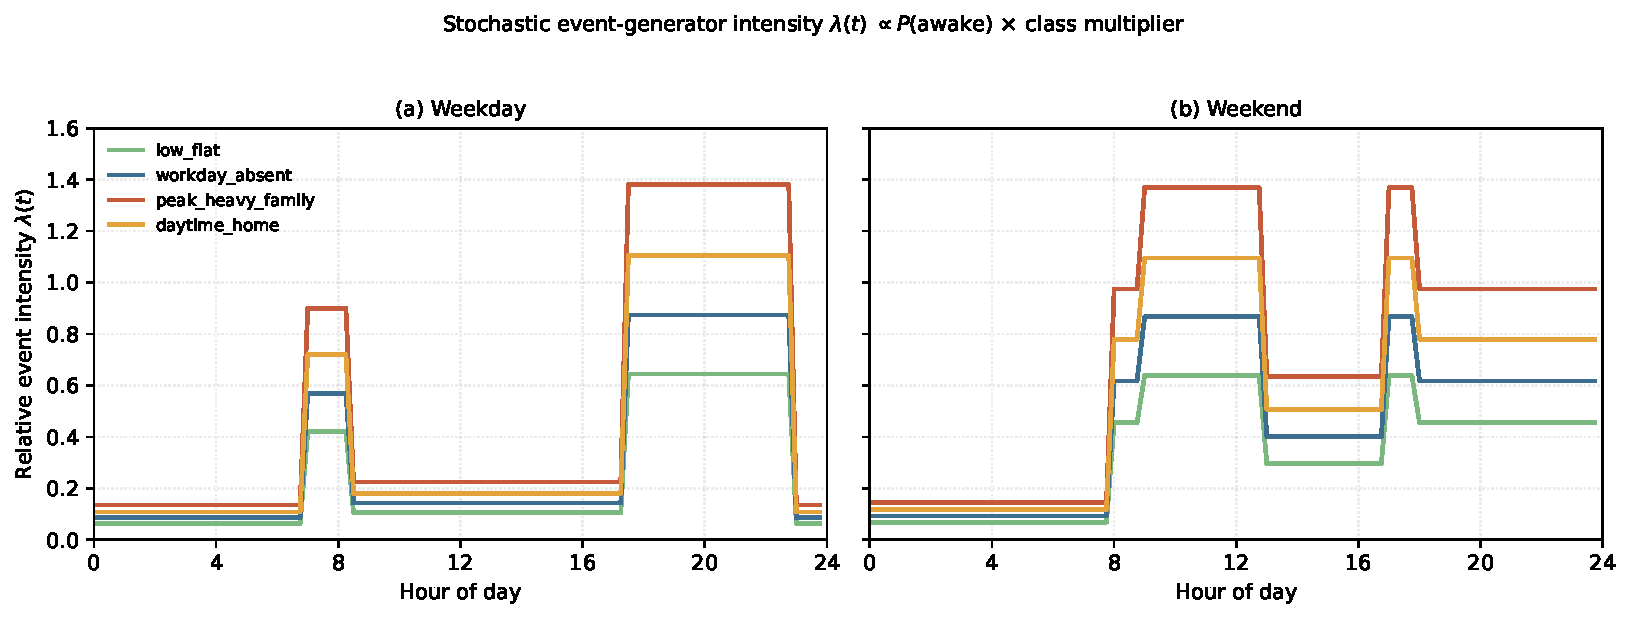
\includegraphics[width=\textwidth]{figures/event_generator_intensity.pdf}
  \caption{Expected event-generator intensity $\lambda(t) \propto P(\text{awake}\mid t) \times m_{\text{class}}$ by hour of day, derived from the occupancy schedule rules in \texttt{occupancy\_model\_spec.yaml} and the four behavioural-class multipliers in \texttt{household\_classifier.py}.}
  \label{fig:event_generator_intensity}
\end{figure}



\subsubsection*{Cohort pipeline}
The canonical cohort is $N=30$ households, which is small enough to keep single-configuration runs and validation workflows tractable. Stochastic spread within a scenario is captured by the realisation pool, which is enumerated as $100$ reproducible seeds (\texttt{seed\_0000}--\texttt{seed\_0099}); each seed generates an independent $N=30$ cohort, so a scenario with $k$ executed seeds aggregates $k \times 30$ household-years of stochastic samples. \Cref{fig:cohort_pipeline} sketches the cohort pipeline.

\begin{figure}[ht]
  \centering
  \resizebox{0.95\textwidth}{!}{%
  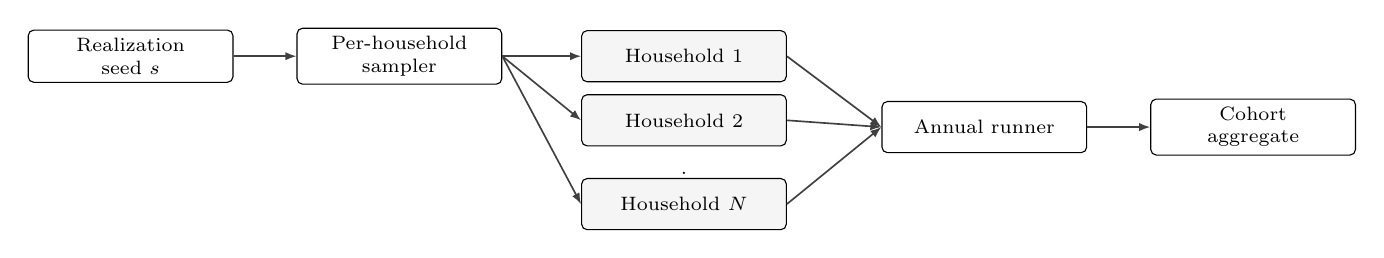
\begin{tikzpicture}[
      every node/.style={font=\scriptsize, align=center, inner sep=3pt},
      box/.style={draw, rounded corners=2pt,
                  minimum height=6.5mm, minimum width=2.6cm},
      stack/.style={box, fill=black!4},
      arrow/.style={-{Latex[length=1.4mm]}, semithick, draw=black!75},
      brace/.style={decorate, decoration={brace, amplitude=4pt}},
  ]
    \node[box] (seed) {Realization\\seed $s$};
    \node[box, right=8mm of seed] (samp) {Per-household\\sampler};
    \node[stack, right=10mm of samp] (hh1) {Household 1};
    \node[stack, below=1.5mm of hh1] (hh2) {Household 2};
    \node[font=\scriptsize, below=0mm of hh2] (dots) {$\vdots$};
    \node[stack, below=4mm of hh2] (hhN) {Household $N$};
    \node[box, right=12mm of hh1, yshift=-9mm] (run) {Annual runner};
    \node[box, right=8mm of run] (agg) {Cohort\\aggregate};
 
    \draw[arrow] (seed) -- (samp);
    \draw[arrow] (samp.east) -- (hh1.west);
    \draw[arrow] (samp.east) -- (hh2.west);
    \draw[arrow] (samp.east) -- (hhN.west);
    \draw[arrow] (hh1.east) -- (run.west);
    \draw[arrow] (hh2.east) -- (run.west);
    \draw[arrow] (hhN.east) -- (run.west);
    \draw[arrow] (run) -- (agg);
 
    \node[font=\scriptsize\itshape, below=2mm of run]
      {};
  \end{tikzpicture}}
  \caption{Stochastic cohort pipeline.}
  \label{fig:cohort_pipeline}
\end{figure}


\subsection{Climate Scenarios}
\label{sec:climateScenariosFramework}

Climate forcing for the scenario-tree leaves is derived from EURO-CORDEX \cite{Jacob2014EuroCordex} regional projections of 2-metre air temperature (\texttt{tas}) and surface solar radiation downwards (\texttt{rsds}). The forcing files described in \Cref{tab:climate_inventory} feed the annual runner through the same forcing-builder layer as the historical Uccle weather, so that the physics, control and systems code paths are identical for historical and future runs.

\subsubsection*{Window definitions} 
The four canonical analysis windows are a baseline ($1981$--$2005$), a near-future window ($2030$--$2049$), a mid-century window ($2050$--$2070$), and a long-term window ($2080$--$2100$), all with inclusive start and inclusive end. The baseline window is bounded above at $2005$ because the EURO-CORDEX historical experiment ends in $2005$, while RCP scenario simulations start in $2006$; aligning the baseline with the historical experiment avoids mixing historical and scenario forcing in the reference climate, while preserving a multi-decadal record that is long enough to characterise baseline thermal forcing. 

\subsubsection*{Pathways and technology pairing} 
Future windows are combined with three RCP pathways (\texttt{rcp\_2\_6}, \texttt{rcp\_4\_5}, \texttt{rcp\_8\_5}), in line with the canonical low/medium/high forcing trilogy \cite{vanVuuren2011}; the baseline window is restricted to the \texttt{historical} pathway. While newer scenario frameworks combine RCPs with Shared Socio-economic Pathways (SSP--RCP, \cite{Riahi2017SSP}), the present work isolates the effect of climate forcing on residential demand, with technology and behaviour treated as separate explicit dimensions of the scenario tree; RCP-only forcing is adequate for the restricted aim of isolating physical climate forcing, provided socio-economic interpretation is limited.

\subsubsection*{Scenarios}
The baseline scenario \texttt{baseline\_1981\_2005\_\_historical\_\_tech\_current\_stock} is a historical-climate reference case: the current Belgian stock representation is exposed to the $1981$--$2005$ historical climate window. It functions as a counterfactual reference for isolating climate and technology effects in \Cref{ch:results}; it is not a reconstruction of actual Belgian residential demand in $1981$--$2005$, because the technology stock of the early $1980$s differs from the current stock represented by \texttt{tech\_current\_stock}. In future windows, \texttt{tech\_frozen\_stock} is used as an explicit climate-only control: it holds the present-day technology representation fixed so that climate effects can be separated from electrification effects. It is not interpreted as a realistic future stock forecast.


\subsection{Climate Uncertainty}
\label{sec:climateUncertainty}

The scenario tree resolves three of the four classical sources of climate-impact uncertainty \cite{Hawkins2009UncertaintyPartitioning}: scenario uncertainty through the RCP pathways, technology/socio-economic uncertainty through the technology cases, and behavioural/internal variability through the stochastic seeds. The fourth source, climate-model structural uncertainty, is \emph{not} resolved: the current scenario tree uses one GCM/RCM chain, as mentioned in \Cref{sec:weatherClimate}. The results of \Cref{ch:results} are therefore conditional on this chain and should be read as such. This is a deliberate scoping choice. The CORDEX archive supports a multi-model ensemble for the same EUR-11 domain \cite{Jacob2014EuroCordex}, and the \texttt{src/climate/} pipeline is parametrised over the GCM/RCM identifiers, so adding more chains is a configuration extension rather than a code change. With $2800$ leaves already enumerated for one chain, adding $k$ additional chains multiplies the experiment space by $k$; the present work treats single-chain experiments as a defensible conditional estimate of demand response and flags multi-chain spread as the primary structural extension for \hyperref[sec:futurework]{future work}.

Two further interpretive notes follow from this scoping. First, the RCP pathways are read as conditional scenarios, not as probabilistic forecasts, consistent with the IPCC framing \cite{IPCC2014SynthesisReport}; no probability weights are attached to RCP\,2.6, RCP\,4.5, RCP\,8.5 in any of the comparisons. Second, the daily temporal resolution of the CORDEX product propagates a known smoothing: sub-daily peak demand is therefore reported only for the historical Uccle path and is not extrapolated to future windows, while daily and seasonal statistics are reported for all windows. \Cref{fig:climateUncertainty_scope} summarises which uncertainty sources are resolved by the scenario tree, and which are not.

\begin{figure}[ht]
  \centering
  \resizebox{0.98\textwidth}{!}{%
  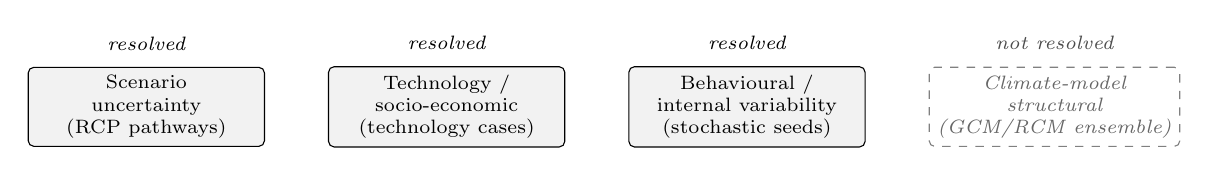
\begin{tikzpicture}[
      every node/.style={font=\scriptsize, align=center, inner sep=3pt},
      box/.style={draw, rounded corners=2pt,
                  minimum height=8mm, minimum width=3.0cm},
      yes/.style={box, fill=black!5},
      no/.style={box, dashed, draw=black!50, text=black!60, font=\scriptsize\itshape},
      arrow/.style={-{Latex[length=1.4mm]}, semithick, draw=black!75},
  ]
    \node[yes] (scen) {Scenario\\uncertainty\\(RCP pathways)};
    \node[yes, right=8mm of scen] (tech) {Technology /\\socio-economic\\(technology cases)};
    \node[yes, right=8mm of tech] (beh)  {Behavioural /\\internal variability\\(stochastic seeds)};
    \node[no,  right=8mm of beh]  (mod)  {Climate-model\\structural\\(GCM/RCM ensemble)};

    \node[font=\scriptsize\itshape, above=1mm of scen] {resolved};
    \node[font=\scriptsize\itshape, above=1mm of tech] {resolved};
    \node[font=\scriptsize\itshape, above=1mm of beh]  {resolved};
    \node[font=\scriptsize\itshape, above=1mm of mod, text=black!70]
      {not resolved};
  \end{tikzpicture}}
  \caption{Sources of climate-impact uncertainty resolved by the scenario tree. The three resolved sources are the RCP pathways, the technology cases, and the stochastic seeds; the unresolved source is climate-model structural uncertainty, which is held fixed at one GCM/RCM chain in the present work.}
  \label{fig:climateUncertainty_scope}
\end{figure}


\subsection{Model Outputs}
\label{sec:modelOutputs}
A single ledger of outputs is produced regardless of which workflow generated the run; the workflow only changes which subset is treated as canonical and, for the scenario tree, which enumerated leaves were actually executed.
\Cref{tab:outputs_inventory} groups the output columns by family. Each column is exposed at the active simulation timestep: hourly for the historical-weather configuration and daily for the processed CORDEX scenario-tree leaves unless an explicit timestep override is configured.

\begin{table}[ht]
  \centering
  \footnotesize
  \caption{Output ledger produced by the systems layer.}
  \label{tab:outputs_inventory}
  \begin{tabular}{@{}l p{0.55\linewidth}@{}}
    \toprule
    \textbf{Family} & \textbf{Columns} \\
    \midrule
    Thermal state and comfort
      & $T_{\text{in,next}}$,
        $Q_{\text{heat,requested}}, Q_{\text{heat,supplied}},
        Q_{\text{heat,max}}, Q_{\text{unmet}}, Q_{\text{excess}}$,
        comfort violation $^{\circ}\text{C}$ and degree-hours \\
    Electricity by end use
      & $P_{\text{el,SH}}, P_{\text{el,DHW}}, P_{\text{el,app}},
         P_{\text{el,light}}, P_{\text{el,cook}}, P_{\text{el,EV}},
         P_{\text{el,total}}$ \\
    Distributed energy
      & $P_{\text{pv}}, P_{\text{el,gross}},
         P_{\text{el,net,grid}}, P_{\text{el,grid,import}},
         P_{\text{el,grid,export}}$ \\
    Non-electric carriers (SH and DHW)
      & $P_{\text{gas}}, P_{\text{oil}}, P_{\text{biomass}},
         P_{\text{propane}}, P_{\text{coal}},
         P_{\text{district\_heat}}$ \\
    Heat-pump diagnostics
      & effective COP, emitter, refrigerant, source/sink
        temperatures, defrost factor, part-load factor,
        capacity-available fraction \\
    Provenance
      & run id, artifact labels, run mode,
        \texttt{scenario\_leaf\_id}, technology case, seed,
        cohort size, config and input hashes
        \cite{Wilkinson2016} \\
    \bottomrule
  \end{tabular}
\end{table}

Three canonical aggregations of this ledger are produced. 
\newline The \emph{deterministic} aggregation is the annual single-household run under one weather year; it is used to inspect end-use shares, seasonal load shape, and comfort under one explicit configuration. 
\newline The \emph{stochastic} aggregation is the per-cohort statistics over the $N$-household sample for one configuration; it is used to characterise diversity, peak coincidence, and the spread of cohort totals. 
\newline The \emph{scenario-tree} aggregation is the same aggregation procedure applied to executed leaves of the four-dimensional tree and joined into a single comparison ledger by the standardised summary layer. The full scenario-tree design enumerates $2800$ possible leaves (\Cref{sec:scenarioTreeSystem}), but the thesis run set executes a targeted subset of $180$ leaves: $100$ full-window climate-only leaves and $80$ hourly design-year leaves. Results in \Cref{ch:results} therefore refer to this executed subset, not to a complete traversal of the full scenario tree.

Each run also writes a \texttt{run\_manifest.json} alongside the data outputs, recording the run mode, timestamp, configuration path and name, reference year, cohort size, random seeds, climate settings, key configured input paths, the resulting output artefact paths, and the git commit hash when the workspace exposes one. The manifest is the operational anchor of the reproducibility contract introduced in \Cref{sec:scenarioTreeSystem}: any output cell can be traced back to its config, inputs, and code state through the manifest alone.

% Climate forcing is derived from EURO-CORDEX simulations driven by Representative Concentration Pathways (RCPs). While newer scenario frameworks combine RCPs with Shared Socioeconomic Pathways (SSPs), the present work focuses on isolating the impact of climate variability on residential energy demand. As such, RCP-based climate projections are sufficient, since socio-economic factors such as building stock evolution and behavioural change are not explicitly modelled. The use of CORDEX ensures that these climate projections are available at a spatial and temporal resolution suitable for building-scale simulation.
% While SSP–RCP combinations are increasingly used in integrated assessment studies, the present work isolates the effect of climate forcing on residential demand. Therefore, RCP-based CORDEX simulations are used without explicit coupling to socio-economic pathways.
% the current scenario tree varies: climate window, RCP pathway, technology case, an stochastic seed
% but it does not yet vary the climate-model chain. So it represents RCP/window uncertainty conditional on one GCM-RCM chain, not the full spread across multiple climate models. A stronger climate uncertainty analysis would add more GCM/RCM chains.

% The baseline is a historical-climate reference case: the current-stock residential technology representation is exposed to the 1981-2005 historical climate window. It is used as a counterfactual reference for isolating climate and technology effects, not as a reconstruction of actual Belgian residential demand in 1981-2005.

% The baseline climate period was defined as 1981–2005 because it lies entirely within the EURO-CORDEX historical experiment, whereas RCP scenario simulations start in 2006. This avoids mixing historical and scenario-forced simulations in the reference climate, while still providing a sufficiently long multi-decadal period for estimating baseline thermal forcing conditions.

% For the stochastic household composition layer, household size was represented using a discrete probability distribution over five occupant classes. The probabilities were selected to be consistent with Belgian household statistics, particularly the high prevalence of one-person households and the national mean household size. Statbel reports that 36.3\% of Belgian private households consisted of one person in 2025, while the average private household size was 2.25 persons \cite{StatbelHouseholds2025}. Therefore, one- and two-person households were treated as common classes, three- and four-person households as moderate classes, and households of five or more persons as a smaller residual category. This residual treatment is also supported by OECD family-composition statistics, which show that households with three or more children form a relatively small share of households in Belgium \cite{OECDFamilySize2024}. The resulting conceptual distribution assigns probabilities of 0.36, 0.31, 0.145, 0.11, and 0.07 to households of size 1, 2, 3, 4, and 5+ respectively.
% %% add occupancy table %%

% The historical baseline uses a current-stock technology representation as the reference technology mix. Future frozen-stock scenarios reuse this same technology representation intentionally as a counterfactual control, not as a realistic forecast of future Belgian household technology. This allows climate-only effects to be separated from technology-transition effects.

% tech\_current\_stock for the baseline.
% \newline tech\_frozen\_stock for future climate-only controls.

% The base model uses 30 households for computationally efficient development, validation, and sensitivity checks. Scenario-tree runs use 100 households because they form the basis for cross-scenario comparison, where aggregate outputs should be less affected by stochastic household sampling noise. The increase from 30 to 100 reduces the expected Monte Carlo sampling error by approximately sqrt(30/100), while remaining computationally tractable for the full scenario ensemble.



%%% --- %%% 
\pagebreak
\section{Validation Strategy}
\label{sec:validation}

This section states what the model is validated against, what it is not validated against, and how each comparison is made. The position taken here is conservative: every validation artefact is labelled by what it actually supports: \emph{calibration}, \emph{internal consistency}, or \emph{external comparison}. A central constraint is the absence of an accessible household-level Belgian smart-meter dataset: no measured per-dwelling load curves were available for direct calibration, so external comparison relies on aggregated representative profiles rather than metered household demand. None of the four layers below is by itself sufficient to claim external validation of the full bottom-up cohort.

\subsection{Layered Validation Framework}
\label{sec:layeredValidation}

No single dataset can validate a bottom-up residential demand model end-to-end. Macro-level statistics constrain annual carrier totals and end-use shares but say nothing about temporal shape. Synthetic references constrain the stochastic structure but cannot pin down absolute magnitudes. Smart-meter samples constrain shape and magnitude jointly but are either representative or small-$N$ case studies, neither of which is a population-level ground truth. Technology-specific references constrain individual submodels but not the full demand stack. The validation strategy therefore stacks four layers, each anchored in an external reference and each evaluated against the same shared \hyperref[sec:validationMetrics]{validation metrics}. A sketch of this stack is shown in \Cref{fig:validation_framework}.

% \begin{figure}[ht]
%   \centering
%   \resizebox{\textwidth}{!}{%
%   \begin{tikzpicture}[
%       every node/.style={font=\scriptsize, align=center, inner sep=3pt},
%       layer/.style={draw, rounded corners=3pt, minimum height=10mm,
%                     minimum width=3.6cm},
%       ref/.style={layer, fill=black!4, font=\scriptsize\itshape,
%                   minimum width=4.2cm},
%       arrow/.style={-{Latex[length=1.4mm]}, semithick, draw=black!75},
%   ]
%     \node[layer] (model) at (0, 0) {\textbf{Model v3 cohort}};

%     \node[layer, right=14mm of model] (macro) {Macro\\(annual totals,\\end-use shares)};
%     \node[layer, below=4mm of macro]   (synth) {Synthetic\\(stochastic\\structure)};
%     \node[layer, below=4mm of synth]   (sm)    {Smart-meter\\(profile shape,\\peak realism)};
%     \node[layer, below=4mm of sm]      (tech)  {Technology\\(PV, EV)};

%     \node[ref, right=12mm of macro] (refm) {Eurostat \texttt{nrg\_d\_hhq};\\Belgian baselines};
%     \node[ref, right=12mm of synth] (refs) {Richardson-style\\reference profiles};
%     \node[ref, right=12mm of sm]    (refr) {Fluvius open data;\\KU\,Leuven 3 houses};
%     \node[ref, right=12mm of tech]  (reft) {PVGIS, Elia ODS032,\\Fluvius EV/PV signature};

%     \draw[arrow] (model.east) -- (macro.west);
%     \draw[arrow] (model.east) -- (synth.west);
%     \draw[arrow] (model.east) -- (sm.west);
%     \draw[arrow] (model.east) -- (tech.west);

%     \draw[arrow] (refm) -- (macro);
%     \draw[arrow] (refs) -- (synth);
%     \draw[arrow] (refr) -- (sm);
%     \draw[arrow] (reft) -- (tech);
%   \end{tikzpicture}}
%   \caption{Four-layer validation framework. Each layer compares one facet of the cohort outputs against an external reference, with the same shared validation metrics applied where applicable.}
%   \label{fig:validation_framework}
% \end{figure}

\begin{figure}[ht]
  \centering
  \resizebox{\textwidth}{!}{%
  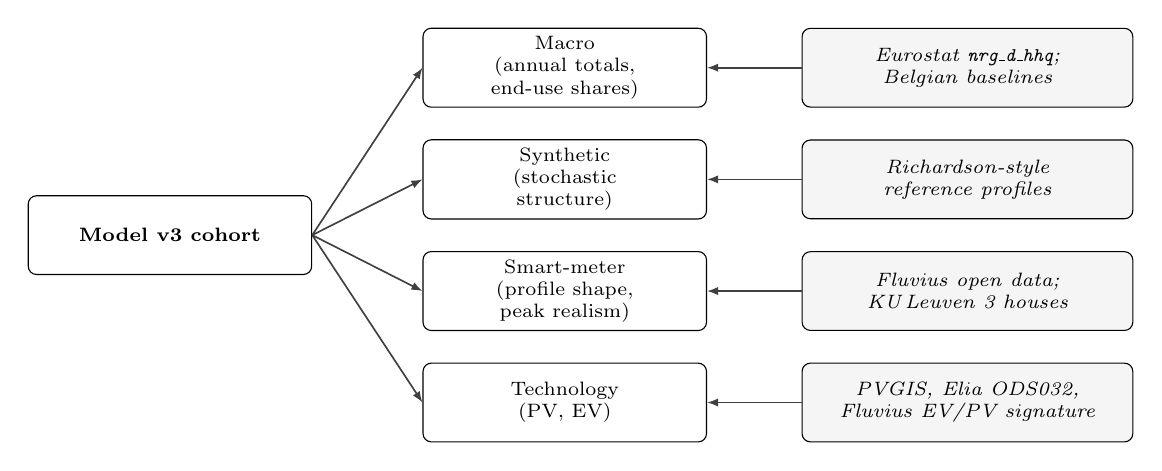
\begin{tikzpicture}[
      every node/.style={font=\scriptsize, align=center, inner sep=3pt},
      layer/.style={draw, rounded corners=3pt, minimum height=10mm,
                    minimum width=3.6cm},
      ref/.style={layer, fill=black!4, font=\scriptsize\itshape,
                  minimum width=4.2cm},
      arrow/.style={-{Latex[length=1.4mm]}, semithick, draw=black!75},
  ]
    %% --- four validation layers, top to bottom ---
    \node[layer] (macro) at (5, 0) {Macro\\(annual totals,\\end-use shares)};
    \node[layer, below=4mm of macro]   (synth) {Synthetic\\(stochastic\\structure)};
    \node[layer, below=4mm of synth]   (sm)    {Smart-meter\\(profile shape,\\peak realism)};
    \node[layer, below=4mm of sm]      (tech)  {Technology\\(PV, EV)};
 
    %% --- model cohort node, vertically centred on the four-layer stack ---
    \node[layer, anchor=east]
      at ($(macro.west)!0.5!(tech.west) - (14mm,0)$)
      (model) {\textbf{Model v3 cohort}};
 
    %% --- reference boxes ---
    \node[ref, right=12mm of macro] (refm) {Eurostat \texttt{nrg\_d\_hhq};\\Belgian baselines};
    \node[ref, right=12mm of synth] (refs) {Richardson-style\\reference profiles};
    \node[ref, right=12mm of sm]    (refr) {Fluvius open data;\\KU\,Leuven 3 houses};
    \node[ref, right=12mm of tech]  (reft) {PVGIS, Elia ODS032,\\Fluvius EV/PV signature};
 
    \draw[arrow] (model.east) -- (macro.west);
    \draw[arrow] (model.east) -- (synth.west);
    \draw[arrow] (model.east) -- (sm.west);
    \draw[arrow] (model.east) -- (tech.west);
 
    \draw[arrow] (refm) -- (macro);
    \draw[arrow] (refs) -- (synth);
    \draw[arrow] (refr) -- (sm);
    \draw[arrow] (reft) -- (tech);
  \end{tikzpicture}}
  \caption{Four-layer validation framework. Each layer compares one
  facet of the cohort outputs against an external reference, with the
  same shared metric battery applied where applicable.}
  \label{fig:validation_framework}
\end{figure}

Two further distinctions are enforced throughout. First, the \emph{role} tag carried in the \hyperref[sec:dataProcessing]{input configuration} prevents a source labelled \texttt{calibration} (the configured Belgian baseline) from being cited as an independent validation reference. Second, the acceptance evaluator separates ``acceptable'' from ``good'' thresholds, so a partial pass is reported as such rather than rounded up to a full success.


\subsection{Validation Metrics}
\label{sec:validationMetrics}
%%% document every error metric used
%%% correlation, RMSE / CVRMSE, NMBE, duration curves, peak error
%%% scale-normalised vs raw comparison
%%% diversity factor / household CV where relevant

A single validation metric is computed wherever a modelled series can be aligned with an external reference. The validation metrics are defined in \texttt{validation/core/} and grouped into five families (\Cref{tab:validation_metrics}). Aggregation horizons are hourly, monthly and annual; spatial scope is per-dwelling or per-cohort depending on the layer.

\begin{table}[ht]
  \centering
  \footnotesize
  \caption{Table of validation metrics. Each metric is computed in the validation core and consumed by the layer runners below. ``Used by'' marks where each metric is actively reported.}
  \label{tab:validation_metrics}
  \begin{tabular}{@{}p{0.18\linewidth} p{0.50\linewidth} p{0.27\linewidth}@{}}
    \toprule
    \textbf{Family} & \textbf{Metric} & \textbf{Used by} \\
    \midrule
    Mean accuracy
      & MBE, MAE, RMSE, CVRMSE
      & macro, synthetic, smart-meter, technology \\
    Temporal structure
      & Pearson $r$; autocorrelation lag-difference;
        peak-timing error (hours); diversity factor
      & synthetic, smart-meter, technology \\
    Variance realism
      & sample variance; coefficient of variation;
        Levene equal-variance test
      & synthetic, smart-meter \\
    Distribution realism
      & two-sample Anderson--Darling statistic;
        LDC overlay; $P_{10}, P_{50}, P_{90}$ errors
      & synthetic, smart-meter \\
    Event behaviour
      & extreme-day extraction; peak-day error; peak MAE
      & smart-meter, technology \\
    End-use decomp
      & per-end-use share; deviation from config baseline
      & macro \\
    \bottomrule
  \end{tabular}
\end{table}

\subsubsection*{Acceptance thresholds}
For an aligned modelled series $m_t$ and reference series $r_t$, the mean bias error is
\begin{equation}
  \mathrm{MBE} = \frac{1}{n}\sum_{t=1}^{n}(m_t-r_t),
\end{equation}
reported in the physical unit of the compared series. Acceptance thresholds are applied to the normalized mean bias error,
\begin{equation}
  \mathrm{NMBE} =
  \frac{\sum_{t=1}^{n}(m_t-r_t)}
       {(n-p)\,\bar r},
\end{equation}
and to
\begin{equation}
  \mathrm{CVRMSE} =
  \frac{1}{\bar r}
  \sqrt{\frac{\sum_{t=1}^{n}(m_t-r_t)^2}{n-p}},
\end{equation}
where $\bar r$ is the reference mean and $p$ is the number of fitted calibration parameters, set to zero for non-calibrated external comparisons.

\subsubsection*{ASHRAE guidelines}
Quantitative acceptance follows an ASHRAE Guideline 14-style policy \cite{ASHRAE14}. Two threshold sets are evaluated jointly: an ``acceptable'' band (monthly $|\mathrm{NMBE}| \le 0.05$, monthly $\mathrm{CVRMSE} \le 0.15$, hourly $|\mathrm{NMBE}| \le 0.10$, hourly $\mathrm{CVRMSE} \le 0.30$, peak MAE $\le \SI{0.2}{kW}$, quantile $P_{10}/P_{90}$ error $\le \SI{0.2}{kW}$) and a tighter \emph{good} band (hourly NMBE $\le 0.05$, hourly CVRMSE $\le 0.20$, peak MAE $\le \SI{0.1}{kW}$, quantile error $\le \SI{0.1}{kW}$). A result that clears the acceptable band but not the good band is reported as acceptable, not as good. CVRMSE thresholds match the range used in IPMVP and other building-performance validation guidelines \cite{IPMVPCoreConcepts2016}.


\subsection{Macro Validation}
\label{sec:macroValidation}
%%% annual structure plausibility
%%% aggregate temporal plausibility
%%% Eurostat + Belgian load context

The macro layer compares annual carrier totals and end-use shares against the configured Belgian residential baseline drawn from Eurostat \cite{EnergyConsumptionHouseholds} through the baseline validation annual runner. Two checks are applied. First, the calibrated annual electricity total is verified
to lie inside the configured BE range (\SI{3500}{kWh} target, range $\SIrange{3000}{3900}{kWh}$; \Cref{tab:macro_benchmark}). Because this total is rescaled to the baseline target at the end of the annual runner (\Cref{sec:deterministicBaselineDemandModel}), this check confirms that the calibration converges, not that the annual total is independently observed. Second, the modelled end-use shares (space heating, DHW, appliances, lighting, cooking) are compared to the Eurostat \texttt{nrg\_d\_hhq} BE shares ($73.01$, $12.00$, plus residual; \Cref{tab:macro_benchmark}); this is an internal consistency check because the model's electricity split is rescaled to those same shares \cite{EnergyConsumptionHouseholds}.

% \begin{figure}[ht]
%   \centering
%   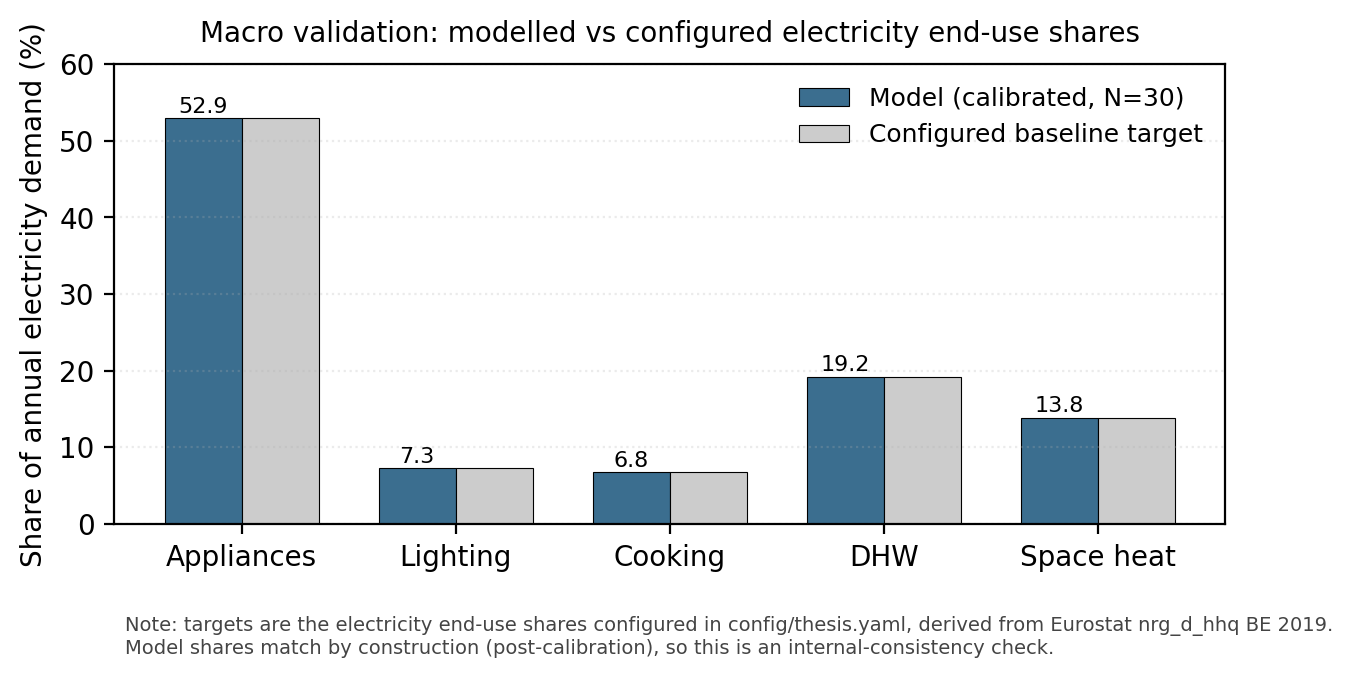
\includegraphics[width=\textwidth]{figures/macro_end_use_shares.png}
%   \caption{Macro validation: modelled cohort electricity end-use shares vs the configured baseline targets (derived from Eurostat \texttt{nrg\_d\_hhq} BE\,2019).}
%   \label{fig:macro_end_use_shares}
% \end{figure}
% Bars match by construction because the model rescales electricity to the configured end-use shares; the figure therefore reports calibration convergence, not external validation.

A full-horizon ($8760$-h) baseline-annual rerun under the thesis configuration, with the envelope calibration of \Cref{sec:modelv3} set to $0.80$ clears all three annual checks: calibrated electricity \SI{3500}{kWh}, useful space-heating thermal demand \SI{15162}{kWh}, and DHW thermal demand \SI{3000}{kWh}, each inside its configured Belgian range. The space-heating total is reported as a thermal baseline calibration, not as an independently validated envelope parameter (\Cref{sec:limitations}).


\subsection{Synthetic Validation}
\label{sec:syntheticValidation}
%%% Richardson / CREST for electricity realism
%%% Fischer et al. for thermal realism
%%% what each benchmark can and cannot support

The synthetic layer exercises the pipeline against a stochastic reference profile whose properties are themselves derived from a generative model rather than a measurement. Two runners cover this layer. The \textit{deterministic synthetic} runner generates a benchmark profile from the configured Belgian baseline bands and feeds the cohort engine through it, primarily as a regression test for the validation pipeline itself. The \emph{Richardson} runner compares the cohort's stochastic baseload structure against Richardson-style domestic profiles \cite{Richardson2010CRESTElectricity,Richardson2010_DomesticHighRes}, which are the canonical synthetic baseline for high-resolution residential electricity modelling. Both runners apply the variance, distribution, and temporal-structure metric families of \Cref{tab:validation_metrics}. The diversity factor computed by \texttt{compute\_diversity\_factor} is the ratio of the sum of individual peaks to the aggregate cohort peak, and is the most sensitive single metric here because it is determined by whether the cohort produces realistic non-coincidence of peak demand.

% % --- fig:synthetic_load_duration_curve ---
% \begin{figure}[ht]
%   \centering
%   \includegraphics[width=0.85\textwidth]
%     {figures/synthetic_load_duration_curve.png}
%   \caption{Synthetic validation: modelled versus synthetic reference load-duration curve.}
%   \label{fig:synthetic_load_duration_curve}
% \end{figure}


% % --- fig:diversity_by_household_count ---
% \begin{figure}[ht]
%   \centering
%   \includegraphics[width=\textwidth]
%     {figures/diversity_by_household_count.png}
%   \caption{Synthetic validation: diversity factor as a function of cohort size, demonstrating the expected convergence toward a stable peak-coincidence value as $N$ grows.}
%   \label{fig:diversity_by_household_count}
% \end{figure}


\subsection{Smart-Meter Validation}
\label{sec:smartMeterValidation}
%%% aggregate realism
%%% distributional realism
%%% UK measured data as external realism check; we don't have anything to pose as "Belgian ground truth"

The smart-meter layer is the only one that compares the cohort directly to observed Belgian residential meter data. It has two sub-tracks because the two available datasets are fundamentally different in cardinality and resolution.

\subsubsection*{Aggregate Fluvius}
The Flemish DSO Fluvius publishes representative \SI{15}{min} residential profiles disaggregated by heat-pump, EV, and PV indicators \cite{Fluvius2024OpenData}. The runner loads the relevant equipment combinations, aggregates them to a representative profile, time-aligns the model cohort to the Brussels timezone, and computes the mean-accuracy, temporal-structure, variance, and distribution metrics of \Cref{tab:validation_metrics}. Acceptance follows the ASHRAE-style thresholds, with explicit external-verdict thresholds added on top (\texttt{CVRMSE\_absolute\_pct $\le 50$}, \texttt{annual\_energy\_error\_pct $\le 25$}, Pearson $\ge 0.5$, $|$peak-timing error$|$ $\le 6\,$h).
% \newline The current persisted artefact reports a \texttt{weak\_failed\_external\_validation} verdict against these thresholds, meaning the aggregate profile is not yet aligned with the Fluvius representative profile. This is reported honestly rather than suppressed: it is the central open validation issue and is treated as such in \Cref{sec:limitations}\footnote{A Fluvius profile is a \emph{representative} category profile, not a measured feeder load, so the verdict supports aggregate profile plausibility rather than distribution-network feasibility.}.

\subsubsection*{High-frequency case study}
The KU\,Leuven three-house dataset \cite{KULeuven3House} provides high-frequency residential meter data for three Belgian dwellings of contrasting EPC and equipment (\Cref{tab:kul_houses}). The runner runs the model in a per-house mode and computes event-realism diagnostics: $24$-hour overlay segments, ramp-rate histograms, and spike-comparison plots. With $N=3$ this layer cannot support a statistical claim; it functions as a high-frequency \emph{event-realism} check, complementary to the aggregate Fluvius layer.

% % --- fig:fluvius_mean_daily_overlay ---
% \begin{figure}[ht]
%   \centering
%   \includegraphics[width=\textwidth]
%     {figures/fluvius_mean_daily_overlay.png}
%   \caption{Smart-meter validation: cohort versus Fluvius representative profile, full $2023$ hourly overlay.}
%   \label{fig:fluvius_mean_daily_overlay}
% \end{figure}


% % --- fig:kuleuven_house1_24h ---
% \begin{figure}[ht]
%   \centering
%   \includegraphics[width=\textwidth]
%     {figures/kuleuven_house1_24h.png}
%   \caption{Smart-meter validation: representative 24-hour segment for KU\,Leuven \texttt{house\_1}, showing event-realism on the high-frequency side.}
%   \label{fig:kuleuven_house1_24h}
% \end{figure}


\subsection{Technology Validation}
\label{sec:technologyValidation}

PV and EV are the two new technology layers added in \hyperref[sec:modelv3]{model v3}. Each is validated against its own references, independently of the household-cohort comparison above.

\subsubsection*{PV triangle}
The PV runner cross-checks the PV submodel against three references. The first leg compares the model's irradiance-to-PV conversion against a $\SI{1}{kWp}$ PVGIS hourly export \cite{Huld2012PVGIS}; the second leg compares the model's daily capacity factor against the Elia ODS032 country-level PV generation series \cite{Elia2024PVODS032}; the third leg compares the cohort PV net-load against the Fluvius residential \emph{with-PV} signature \cite{Fluvius2024OpenData}. The persisted artefact reports a Pearson correlation of $0.998$ on the PVGIS leg ($\text{hourly CF MAE} = 0.011$), a daily-CF correlation of $0.976$ on the Elia leg, and a monthly mean-absolute capacity-factor error of about $25\,\%$, which is consistent with single-chain modelling against country aggregate PV \cite{Pfeifroth2018SARAH}.

% % --- fig:pv_pvgis_reference ---
% \begin{figure}[ht]
%   \centering
%   \includegraphics[width=\textwidth]
%     {figures/pv_pvgis_reference.png}
%   \caption{PV validation: physical-reference leg of the model's irradiance-to-PV conversion against the PVGIS hourly \SI{1}{kWp} export, with hourly Pearson $r = 0.998$.}
%   \label{fig:pv_pvgis_reference}
% \end{figure}


% % --- fig:pv_elia_capacity_factor ---
% \begin{figure}[ht]
%   \centering
%   \includegraphics[width=\textwidth]
%     {figures/pv_elia_capacity_factor.png}
%   \caption{PV validation: Elia ODS032 Belgian country-level PV capacity factor for $2023$, with daily capacity-factor correlation $\approx 0.976$.}
%   \label{fig:pv_elia_capacity_factor}
% \end{figure}

\subsubsection*{EV}
The EV runner compares the model EV home-charging profile against the Fluvius \emph{EV signature} constructed as the difference between the EV-no-PV and no-EV-no-PV representative profiles. The persisted artefact reports a mean-daily Pearson correlation of $0.946$, a peak-hour match at \texttt{01:00}, and an annual-energy gap of $-43\,\%$ against the Fluvius positive EV increment ($\SI{2626}{kWh}$ per reference meter), which closes to $-1\,\%$ under a sensitivity that rescales annual home-charging to $\SI{2600}{kWh}$ while preserving the model timing shape. This is treated as a category-profile signature check, not as a session-level charging validation \cite{Fluvius2024OpenData}.

% % --- fig:ev_signature ---
% \begin{figure}[ht]
%   \centering
%   \includegraphics[width=\textwidth]
%     {figures/ev_fluvius_signature.png}
%   \caption{EV technology validation: mean-daily overlay of the Fluvius residential EV signature versus the model EV home-charging profile.}
%   \label{fig:ev_signature}
% \end{figure}


\subsection{Validation Summary}
\label{sec:validationSummary}

\Cref{tab:validation_summary} consolidates what each layer supports, the reference dataset, and the most informative metric family. Two honest constraints follow from this table. First, the macro layer is internal-consistency, not external validation, because the calibration target is also the comparison target. Second, the aggregate Fluvius layer is the strictest external profile-shape test and is therefore treated as the central validation stress test in \Cref{ch:results}; until that comparison is evaluated, smart-meter realism is interpreted through both the aggregate Fluvius profile and the KU\,Leuven event-realism case study.

\begin{table}[ht]
  \centering
  \footnotesize
  \caption{Validation matrix. Each row maps one layer to its reference dataset, the family of metrics evaluated, and what the layer does and does not support.}
  \label{tab:validation_summary}
  \begin{tabular}{@{}p{0.18\linewidth} p{0.22\linewidth}
                   p{0.18\linewidth} p{0.32\linewidth}@{}}
    \toprule
    \textbf{Layer} & \textbf{Reference} &
      \textbf{Primary metric} & \textbf{Supports / does not support} \\
    \midrule
    Macro
      & Eurostat \texttt{nrg\_d\_hhq} BE shares
        \cite{eurostat_disaggregated_nodate}
      & end-use share error
      & supports annual calibration convergence; does not support
        external validation \\
    Synthetic / Richardson
      & Richardson-style stochastic profile
        \cite{Richardson2010CRESTElectricity}
      & variance, $r$, diversity factor
      & supports stochastic structure plausibility; does not
        constrain absolute magnitudes \\
    Smart-meter aggregate
      & Fluvius representative profiles
        \cite{Fluvius2024OpenData}
      & CVRMSE, peak-timing, Anderson--Darling
      & currently fails the external verdict; treated as open issue \\
    Smart-meter high-frequency
      & KU\,Leuven three-house dataset
        \cite{KULeuven3House}
      & ramp histogram, peak MAE
      & supports event-realism qualitatively; $N=3$ precludes a
        statistical claim \\
    PV triangle
      & PVGIS \cite{Huld2012PVGIS}, Elia ODS032
        \cite{Elia2024PVODS032}
      & hourly $r$, daily CF
      & supports PV submodel; does not validate cohort
        self-consumption \\
    EV
      & Fluvius EV signature \cite{Fluvius2024OpenData}
      & daily $r$, peak-hour match
      & supports EV signature shape; does not validate session-level
        charging \\
    \bottomrule
  \end{tabular}
\end{table}



\mode<all> % do not remove

    \chapterOrPart{Results}\label{ch:results}

\begin{explanation}
    It is mandatory to report the obtained results from modelling work, calculations, simulations and experiments.
    
    The guidelines for formatting figures, tables and mathematical expressions can be found in the appendix on formatting.
    
    Feel free to alter the name of the chapter and/or the sections.
\end{explanation}

% The framing of this chapter follows directly from the validation posture established in \Cref{sec:validation}: the model supports exploratory scenario comparison and stress testing, not calibrated national forecasting. Results are therefore reported as conditional projections under the four scenario-tree dimensions of \Cref{sec:scenarioTreeSystem}, each with a stable \texttt{scenario\_leaf\_id} that can be traced back to its configuration, inputs, and code state. Where the underlying artefact carries a quality caveat, the caveat is reported alongside the number.


\section{Final Model}
\label{sec:finalModel}

The final model used in this thesis is Model v3: a stochastic, physics-informed bottom-up residential demand model with explicit carrier accounting, PV and EV modules, and scenario-tree provenance. The model design enumerates a full four-dimensional scenario space of $2800$ leaves, but the thesis results are based on the executed subset available in the run registries. This distinction is important: the tree defines the reproducible experiment space, whereas only executed leaves constitute numerical evidence in this chapter.


\subsection{Canonical Execution Sets}
\label{sec:resultConfigs}

Three execution sets are used; as listed in \Cref{tab:canonical_configurations}. The first is the canonical thesis configuration, used for the annual baseline and validation runs under the 2023 historical-weather configuration. The second is the main scenario-tree ledger under \texttt{experiments/scenario\_tree}, which provides full-window climate-only comparisons for the current/frozen-stock technology cases. The third is the \texttt{scenario\_tree\_output34} design-year execution set, which provides stochastic hourly cohort runs for selected peak, diversity, and technology-stress comparisons.

\begin{table}[ht]
  \centering
  \footnotesize
  \caption{Executed model configurations used in the results chapter.}
  \label{tab:canonical_configurations}
  \begin{tabular}{@{}p{0.22\linewidth} p{0.23\linewidth}
                  p{0.23\linewidth} p{0.23\linewidth}@{}}
    \toprule
    \textbf{Setting} & \textbf{Validation config}
      & \textbf{Main scenario tree} & \textbf{Scenario set} \\
    \midrule
    Main artefact
      & \texttt{config/thesis.yaml}
      & \texttt{scenario\_tree}
      & \texttt{scenario\_tree\_output34} \\
    Purpose
      & baseline and validation checks
      & climate-only scenario comparison
      & peak, diversity, and technology-stress comparison \\
    Weather / climate
      & RMI/PVGIS 2023
      & processed CORDEX windows
      & selected CORDEX design years \\
    Active timestep
      & hourly
      & native daily CORDEX cadence
      & hourly; daily CORDEX forcing forward-filled \\
    Household treatment
      & $N=30$ for cohort validation; deterministic annual baseline where applicable
      & stock-weighted archetype / summary ledger
      & stochastic cohort, $N=30$ \\
    Executed evidence
      & full-horizon validation artefacts
      & $100$ latest-successful leaves
      & $80$ latest-successful leaves \\
    Technology coverage
      & current thesis stock
      & current/frozen stock
      & current, frozen, moderate electrification, high electrification + PV + EV \\
    \bottomrule
  \end{tabular}
\end{table}

\subsection{Experimental Coverage}
\label{sec:experimentalCoverage}

The scenario-tree schema enumerates $100$ historical baseline leaves and
$2700$ future leaves, for $2800$ leaves in total. The current thesis evidence consists of $180$ distinct latest-successful scenario leaves: $100$ leaves from the main \texttt{scenario\_tree} registry and $80$ leaves from the \texttt{scenario\_tree\_output34} registry. The main registry covers the baseline current-stock case and frozen-stock future controls across all three RCP pathways and all future climate windows with ten realizations per scenario group. The \texttt{output34} registry adds selected design-year stochastic cohort runs, including moderate and high electrification technology cases with five realizations per design-year group.
\newline The remaining leaves are part of the reproducible experiment design but are not used as executed evidence. Scenario results are therefore interpreted as a targeted exploration of climate and technology contrasts.

% \begin{table}[ht]
%   \centering
%   \footnotesize
%   \caption{Scenario-tree execution coverage used as numerical evidence.}
%   \label{tab:experimental_coverage}
%   \begin{tabular}{@{}l r r l@{}}
%     \toprule
%     \textbf{Registry} & \textbf{Enumerated space} &
%       \textbf{Latest-successful leaves} & \textbf{Role in thesis} \\
%     \midrule
%     \texttt{scenario\_tree}
%       & $2800$ leaves & $100$
%       & full-window climate-only comparison \\
%     \texttt{scenario\_tree\_output34}
%       & targeted design-year subset & $80$
%       & peak, diversity, and technology-stress comparison \\
%     \midrule
%     Combined executed evidence
%       & -- & $180$
%       & basis for scenario results reported in this chapter \\
%     \bottomrule
%   \end{tabular}
% \end{table}


\subsection{Validation Results}
\label{sec:resultValidation}

\Cref{tab:validation_results_summary} summarises the validation evidence used
to interpret the results. The table is deliberately conservative: calibration
checks, synthetic structural checks, measured-profile comparisons, and
technology-specific validation are not treated as equivalent forms of evidence.

\begin{table}[ht]
  \centering
  \footnotesize
  \caption{Validation headline metrics used to interpret the final model results.}
  \label{tab:validation_results_summary}
  \begin{tabular}{@{}p{0.20\linewidth} p{0.23\linewidth}
                  p{0.31\linewidth} p{0.18\linewidth}@{}}
    \toprule
    \textbf{Layer} & \textbf{Reference} &
      \textbf{Headline metric} & \textbf{Verdict} \\
    \midrule
    Annual baseline
      & Belgian annual targets / Eurostat shares
        \cite{eurostat_disaggregated_nodate}
      & Electricity \SI{3500}{kWh}; space-heating thermal
        \SI{15162}{kWh}; DHW thermal \SI{3000}{kWh};
        end-use share error $\approx 0$
      & calibration convergence\\
    Synthetic / Richardson
      & Richardson-style baseload
        \cite{Richardson2010CRESTElectricity}
      & synthetic Pearson $r=0.760$; synthetic diversity factor $3.22$;
        Richardson diversity factor $3.40$ vs $3.82$ reference
      & stochastic structure plausible; not Belgian empirical proof \\
    Smart-meter aggregate
      & Fluvius representative profiles \cite{Fluvius2024OpenData}
      & CVRMSE $\approx \SI{88}{\percent}$; Pearson $r \approx 0.40$;
        annual-energy error $\approx \SI{56}{\percent}$;
        peak-timing error $\approx 18$ h
      & failed external profile-shape check\\
    Smart-meter high-frequency
      & KU\,Leuven three-house case study \cite{KULeuven3House}
      & hourly model cannot reproduce household-level sub-hourly spikes
      & event-realism diagnostic; $N=3$ precludes population claim \\
    PV physical reference
      & PVGIS \cite{Huld2012PVGIS}
      & hourly $r=0.998$; hourly capacity-factor MAE $=0.011$;
        annual specific-yield error $\approx \SI{9}{\percent}$
      & strong physical-reference agreement \\
    PV country reference
      & Elia ODS032 \cite{Elia2024PVODS032}
      & daily capacity-factor correlation $r \approx 0.976$;
        monthly mean-absolute CF error $\approx \SI{25}{\percent}$
      & strong daily shape; monthly magnitude imperfect \\
    PV residential signature
      & Fluvius PV signature \cite{Fluvius2024OpenData}
      & mean-daily correlation $\approx 0.48$
      & moderate signature agreement \\
    EV residential signature
      & Fluvius EV signature \cite{Fluvius2024OpenData}
      & mean-daily $r=0.946$; peak hour \texttt{01:00};
        annual-energy gap $-\SI{43}{\percent}$, closing to
        $\approx -\SI{1}{\percent}$ under the \SI{2600}{kWh/yr} sensitivity
      & timing strong; magnitude requires sensitivity \\
    \bottomrule
  \end{tabular}
\end{table}

The resulting validation posture is mixed. Annual calibration and the PV and EV technology signatures justify using the model for conditional scenario experiments, but the unresolved Fluvius aggregate-profile mismatch means it cannot be presented as an externally calibrated Belgian smart-meter profile model. The scenario results that follow are therefore read as traceable conditional projections under the stated configuration rather than calibrated forecasts of Belgian residential load.


\pagebreak
\section{Climate Scenario Results}
\label{sec:climateScenarioResults}

This section reports the executed subset of the scenario tree. Climate-pressure and annual heating-change results draw on the 100 successful full-window leaves (daily cadence; ten realizations per scenario group); peak-load and grid-stress results draw on the 80 successful design-year leaves in \texttt{scenario\_tree\_output34}, which run hourly 30-household stochastic cohorts with five realizations per design-year group. Neither ledger includes active cooling final energy, so cooling is treated as a demand-pressure indicator only.


\subsection{Physical Impact}
\label{sec:physicalImpact}

The physical climate signal is isolated under \texttt{tech\_frozen\_stock},
which holds the dwelling and technology stock fixed so that changes in the
heating and cooling indicators reflect the imposed climate window and pathway
rather than electrification. \Cref{tab:climate_degree_days_results} reports
annualized HDD$_{18}$ and CDD$_{22}$ from the full-window summaries alongside
the paired annual useful-heating change.

\begin{table}[ht]
  \centering
  \footnotesize
  \caption{Climate-pressure and useful-heating response under the frozen-stock climate-only comparison. HDD$_{18}$ and CDD$_{22}$ are annualized degree-day means; useful-heating change is the paired annual mean from the full-window summary layer.}
  \label{tab:climate_degree_days_results}
  \begin{tabular}{@{}l l r r r r r@{}}
    \toprule
    \textbf{Window} & \textbf{Pathway} &
    \textbf{HDD$_{18}$} & $\Delta$\textbf{HDD$_{18}$} &
    \textbf{CDD$_{22}$} & $\Delta$\textbf{CDD$_{22}$} &
    $\Delta Q_{\text{heat}}$ \\
    & & ($^{\circ}$C d/yr) & (\%) & ($^{\circ}$C d/yr) & ($^{\circ}$C d/yr) & (\%) \\
    \midrule
    1981--2005 & historical & 3341 & +0.0 & 14.3 & +0.0 & +0.0 \\
    2030--2049 & RCP 2.6 & 3009 & -9.9 & 40.3 & +26.0 & -10.1 \\
    2030--2049 & RCP 4.5 & 3071 & -8.1 & 24.2 & +9.9 & -8.5 \\
    2030--2049 & RCP 8.5 & 3034 & -9.2 & 21.2 & +6.9 & -9.7 \\
    2050--2070 & RCP 2.6 & 3017 & -9.7 & 31.4 & +17.1 & -7.3 \\
    2050--2070 & RCP 4.5 & 2846 & -14.8 & 50.9 & +36.6 & -13.6 \\
    2050--2070 & RCP 8.5 & 2718 & -18.7 & 59.0 & +44.6 & -19.9 \\
    2080--2100 & RCP 2.6 & 3073 & -8.0 & 31.9 & +17.6 & -5.9 \\
    2080--2100 & RCP 4.5 & 2803 & -16.1 & 44.7 & +30.3 & -16.2 \\
    2080--2100 & RCP 8.5 & 2306 & -31.0 & 109.3 & +94.9 & -33.3 \\
    \bottomrule
  \end{tabular}
\end{table}

\subsubsection*{Change in degree days}
The strongest executed climate-pressure case is \texttt{long\_term\_2080\_2100} under RCP\,8.5. Relative to the historical baseline, HDD$_{18}$ falls from about $3341$ to $2306\,^{\circ}\mathrm{C}\cdot\mathrm{d}$ per year ($-31.0\,\%$; \Cref{fig:phase1_hdd_pct_heatmap}), while CDD$_{22}$ rises from $14.3$ to $109.3\,^{\circ}\mathrm{C}\cdot\mathrm{d}$ per year (\Cref{fig:phase1_cdd_abs_heatmap}). The pathway ordering is not monotonic in every near-future cell of this single GCM--RCM chain, so the robust statement is directional and conditional: warming reduces heating pressure and increases cooling pressure, with the largest response in the long-term RCP\,8.5 cell.

\begin{figure}[ht]
  \centering
  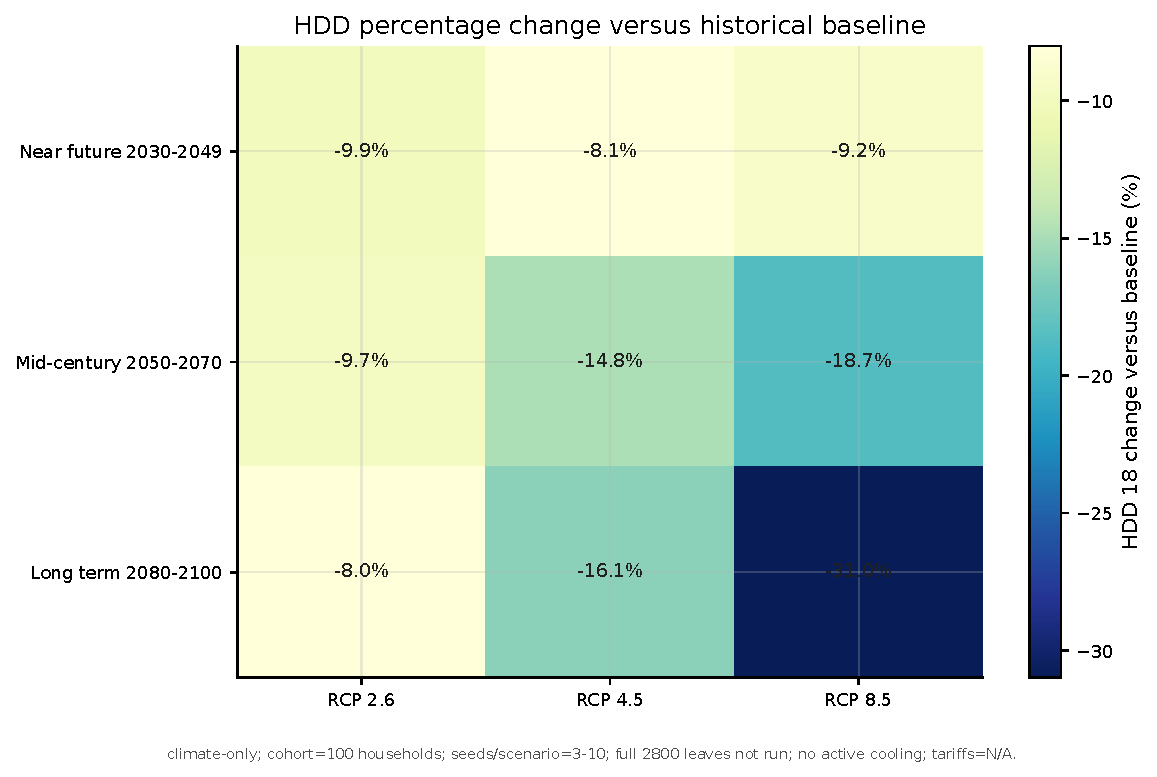
\includegraphics[width=0.8\textwidth]
    {figures/phase1_hdd_pct_decrease_heatmap.pdf}
  \caption{HDD$_{18}$ percentage decrease across climate window $\times$ RCP pathway, relative to the historical baseline window. The long-term RCP\,8.5 cell shows the strongest executed reduction, consistent with the $-31.0\,\%$ headline in \Cref{tab:climate_degree_days_results}.}
  \label{fig:phase1_hdd_pct_heatmap}
\end{figure}

\begin{figure}[ht]
  \centering
  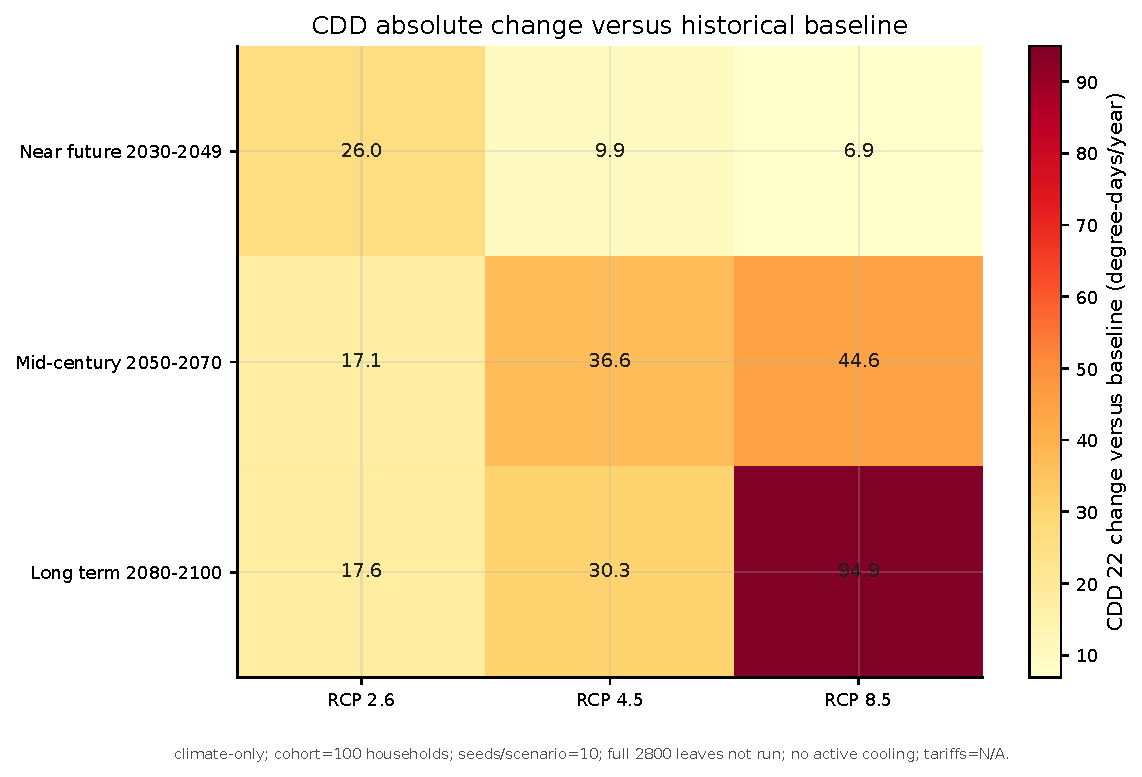
\includegraphics[width=0.8\textwidth]{figures/phase1_cdd_abs_increase_heatmap.pdf}
  \caption{CDD$_{22}$ absolute increase across climate window $\times$ RCP pathway, relative to the historical baseline window. CDD$_{22}$ rises from a small base; the long-term RCP\,8.5 cell reaches about $+94.9\,^{\circ}\mathrm{C}\cdot\mathrm{d}$ per year.}
  \label{fig:phase1_cdd_abs_heatmap}
\end{figure}

\subsubsection*{Useful heating demand}
The useful-heating response follows the same broad direction as HDD$_{18}$: all frozen-stock future cells reduce annual useful-heating demand relative to the paired historical baseline. The response is not perfectly ordered across all near-future pathway cells, which is expected for one regional climate-model chain and finite window samples. The strongest reduction again occurs in the long-term RCP\,8.5 cell, where useful heating falls by about $33.3\,\%$ in the full-window comparison (\Cref{fig:phase1_sh_pct_heatmap}).

\begin{figure}[ht]
  \centering
  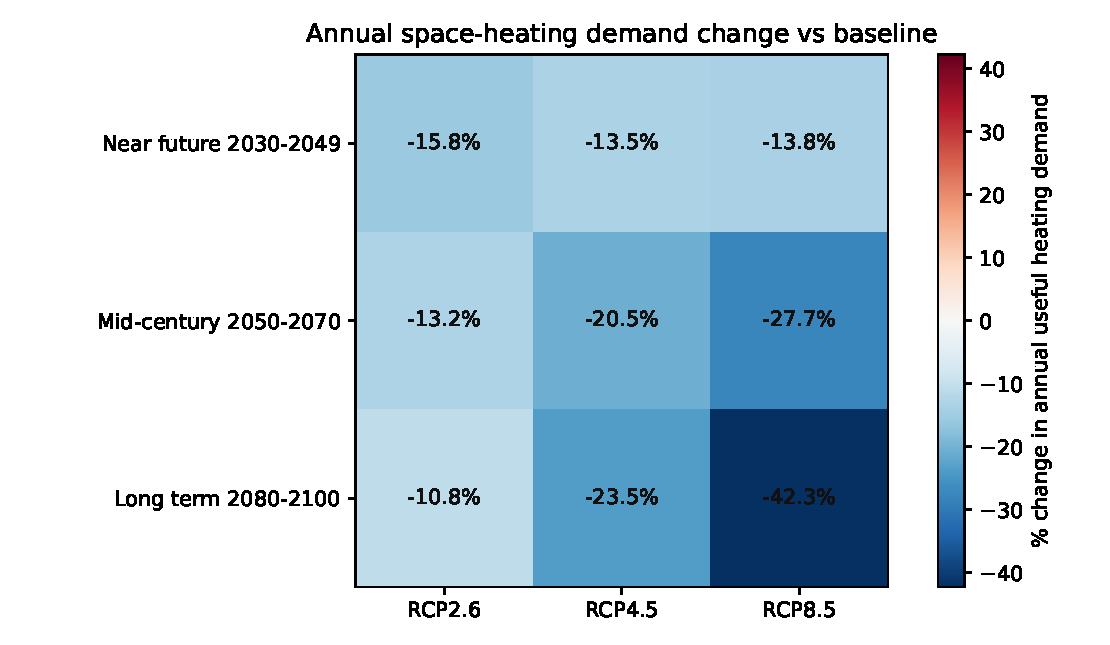
\includegraphics[width=0.8\textwidth]{figures/annual_space_heating_percentage_heatmap.pdf}
  \caption{Annual useful space-heating percentage change across climate window $\times$ RCP pathway under \texttt{tech\_frozen\_stock}. All executed future cells reduce useful-heating demand relative to the paired historical baseline, with the strongest reduction in long-term RCP\,8.5.}
  \label{fig:phase1_sh_pct_heatmap}
\end{figure}

\subsubsection*{Climate change physical results}
These results support a clear but limited conclusion. Climate change reduces modelled space-heating pressure under fixed stock, but the model does not translate higher CDD into active cooling electricity. The cooling result is therefore a demand-pressure result, not a forecast of cooling load.


\subsection{System Impact}
\label{sec:systemImpact}

Peak-grid results are taken from the hourly design-year runs because peak import, load duration and threshold exceedance are hourly quantities. \Cref{tab:peak_grid_import_results} reports the cold-design-year stress case for the historical baseline and the long-term RCP\,8.5 cases.

\begin{table}[ht]
  \centering
  \footnotesize
  \caption{Cold-design-year grid-stress results for the hourly 30-household runs.}
  \label{tab:peak_grid_import_results}
  \resizebox{\textwidth}{!}{%
  \begin{tabular}{@{}l l r r r r r@{}}
    \toprule
    \textbf{Technology case} & \textbf{Climate case} &
    \textbf{Grid import} & \textbf{Gas} &
    \textbf{Peak import} & $\Delta$\textbf{peak} &
    \textbf{Hours > threshold} \\
    & & (kWh/hh/yr) & (kWh/hh/yr) & (kW) & (\%) & (h/yr) \\
    \midrule
    \texttt{current\_stock} & baseline / historical & 5845 & 19406 & 30.80 & +0.0 & 1968 \\
    \texttt{frozen\_stock} & 2080--2100 / RCP 8.5 & 5249 & 13934 & 30.58 & -0.7 & 1424 \\
    \texttt{moderate\_electrification} & 2080--2100 / RCP 8.5 & 18497 & 9063 & 106.45 & +245.6 & 6985 \\
    \texttt{high\_electrification\_pv\_ev} & 2080--2100 / RCP 8.5 & 34285 & 1894 & 188.40 & +511.7 & 8760 \\
    \bottomrule
  \end{tabular}}
\end{table}

\subsubsection*{Peak grid import}
Across the executed design-year subset, technology choice dominates climate forcing for peak grid import. Under frozen stock, long-term RCP\,8.5 leaves the cohort peak almost unchanged ($30.80$ to $30.58$ kW), whereas switching the technology case under the same forcing lifts it to $106.45$ kW under moderate electrification and $188.40$ kW under high electrification with PV and EV.

\subsubsection*{Threshold exceedance}
The threshold-hour metric is a stress diagnostic relative to the configured cohort threshold rather than a prediction of distribution-grid failure. It remains informative: under the current threshold definition, the electrified cases exceed the historical stress band for most or all hours of the design year.


\subsection{Economic and Emissions Impact}
\label{sec:economicImpact}

The economic and emissions figures are conditional accounting outputs under the configured tariff, CAPEX and emission-factor assumptions, and should not be read as policy forecasts. 

\subsubsection*{Economics}
In the cold-design-year long-term RCP\,8.5 case, the dynamic-tariff bill falls from about € 4082 per household in the historical current-stock baseline to € 3351 under frozen stock, because gas demand falls with heating pressure. The same tariff raises bills to about € 6892 under moderate electrification and € 10965 under the high-electrification PV--EV case. Across the executed tariff scenarios, electrification remains more expensive under the current tariff, export-credit and capex assumptions; the current outputs therefore should not be framed as showing favourable electrification economics.

\subsubsection*{Emissions}
Operational emissions use a fixed electricity-emission factor. Under that assumption, frozen stock falls to about $3602$ kgCO$_2$/household/year ($-24.9\,\%$), moderate electrification falls slightly to about $4605$ kgCO$_2$/household/year ($-4.0\,\%$), and the high-electrification PV--EV case rises to about $5525$ kgCO$_2$/household/year ($+15.2\,\%$). This result is sensitive to the fixed electricity factor and should be interpreted as a scenario-accounting result, not as a general decarbonisation conclusion.


\subsection{Sensitivity and Uncertainty}
\label{sec:sensitivityStochasticRobustness}

The executed design-year scenario results contain five stochastic seeds per selected scenario/design-year group, and the comparison files report P10/P50/P90 bands across those seeds. The full-window climate-only results use ten paired realizations per scenario group.

The EV annual-energy sensitivity exists in the validation artifacts and shows that the base EV profile uses about $1491$ kWh per active EV per year versus a Fluvius-derived reference of about $2626$ kWh/year ($-43.2\,\%$), while the $2600$ kWh/year sensitivity closes the annual gap to about $-1.0\,\%$ without changing the mean-daily timing correlation. Scenario results involving \texttt{tech\_high\_electrification\_pv\_ev} should therefore be read as conditional on the configured EV charging magnitude.

Finally, all climate results remain conditional on the single CORDEX chain used here. The executed tree samples pathways, windows, technology cases and seeds, but it does not sample inter-model climate uncertainty.
\mode<all> % do not remove

    \chapterOrPart{Discussion}\label{ch:discussion}

\begin{explanation}
    It is mandatory to discuss the obtained results. But it must not necessarily be done in a separate chapter. It can also be part of the chapter with results.
    
    Feel free to alter the name of the chapter and/or the sections.
\end{explanation}

\section{Adaptation Insight}
\label{sec:adaptationInsight}

The results of \Cref{ch:results} reframe the residential demand problem. The executed climate-only cases show declining heating pressure and rising cooling pressure, while the hourly design-year cases show that electrification, not climate forcing alone, dominates peak grid import. Adaptation is therefore treated here as a set of directions supported by the modelled patterns because active cooling final energy is not included, and the investment outputs use illustrative tariff, emission-factor, CAPEX, and O\&M assumptions.


\subsection{Combined Heating/Cooling Service}
\label{sec:adaptation_reversible_hp}

The rise in CDD$_{22}$ from about $14.3$ to $109.3\,^{\circ}\mathrm{C}\cdot\mathrm{d}$ per year under long-term RCP\,8.5 (\Cref{tab:climate_degree_days_results}) makes cooling service a relevant adaptation dimension. The current model does not simulate active cooling electricity, so reversible heat pumps cannot be evaluated as a fully modelled cooling technology. Instead, the investment-adaptation layer reports a service proxy: it combines the cooling-pressure indicator with the technology option’s ability to provide reversible cooling.

\subsubsection*{Reversible-heat-pump adaptation}
\Cref{fig:reversible_hp_adaptation_proxy} should therefore be read as a prioritisation proxy, not as an economic proof that reversible heat pumps outperform heating-only heat pumps. In the current tariff and CAPEX assumptions, the reversible option carries additional annualized cost relative to the air-water heating-only option because the bill ledger does not yet monetize cooling comfort. Its value in this chapter is more specific: it identifies where the heating-to-cooling transition makes a cooling-capable heat-pump configuration the relevant adaptation option to test in the next model version.

\begin{figure}[ht]
  \centering
  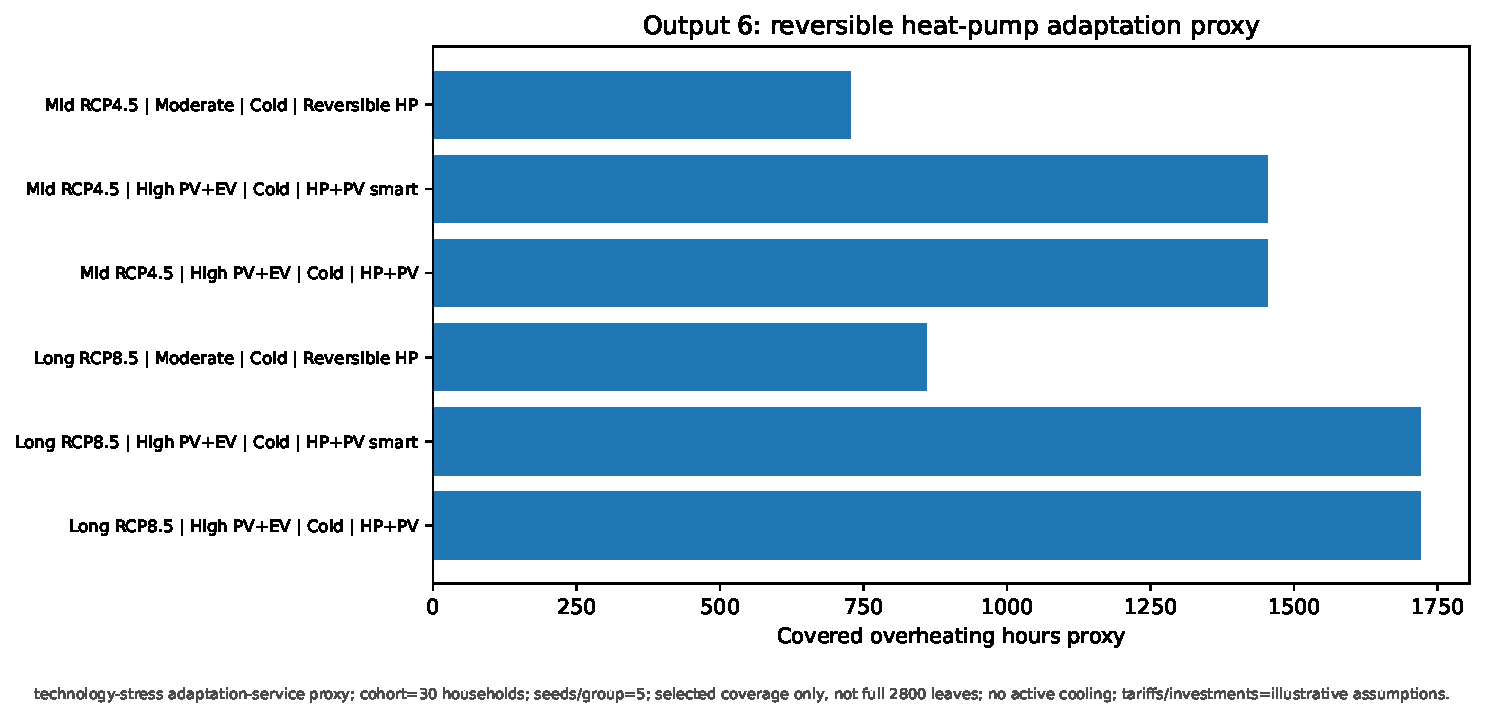
\includegraphics[width=0.9\textwidth]{figures/output6_reversible_hp_adaptation_proxy.pdf}
  \caption{Reversible-heat-pump adaptation-service proxy. The proxy is based on cooling-exposure indicators and technology service capability.}
  \label{fig:reversible_hp_adaptation_proxy}
\end{figure}


\subsection{PV Adaptation}
\label{sec:adaptation_pv_self_consumption}

PV adaptation is interpreted through self-consumption rather than installed capacity alone. \Cref{fig:pv_scr_ssr} reports the PV self-consumption ratio (SCR) and self-sufficiency ratio (SSR) for the executed design-year scenarios, where:
\begin{equation}
    \text{SCR} = \frac{E_\text{PV,self-consumed}}{E_\text{PV,total}}, 
    \quad 
    \text{SSR} = \frac{E_\text{PV,self-consumed}}{E_\text{load,total}}
\end{equation}
The high-electrification PV--EV case raises SCR because heat-pump and EV loads absorb a larger fraction of local generation. In the cold-design long-term RCP\,8.5 case, SCR rises from about $0.37$ under frozen stock to about $0.48$ under moderate electrification and $0.62$ under the high-electrification PV--EV case.

\subsubsection*{PV Self-consumption limitations}
\Cref{fig:pv_scr_ssr} also shows the limitation. SSR remains very low in the electrified cases because the electrified load is much larger than the modelled PV generation. PV therefore improves local use of generated electricity, but in the current scenario set it does not remove the peak-grid problem identified in \Cref{sec:systemImpact}. Under low or zero export value, this makes self-consumption timing more important than export credit; it does not make the high-electrification case economically favourable under the current post-processing assumptions.

\begin{figure}[ht]
  \centering
  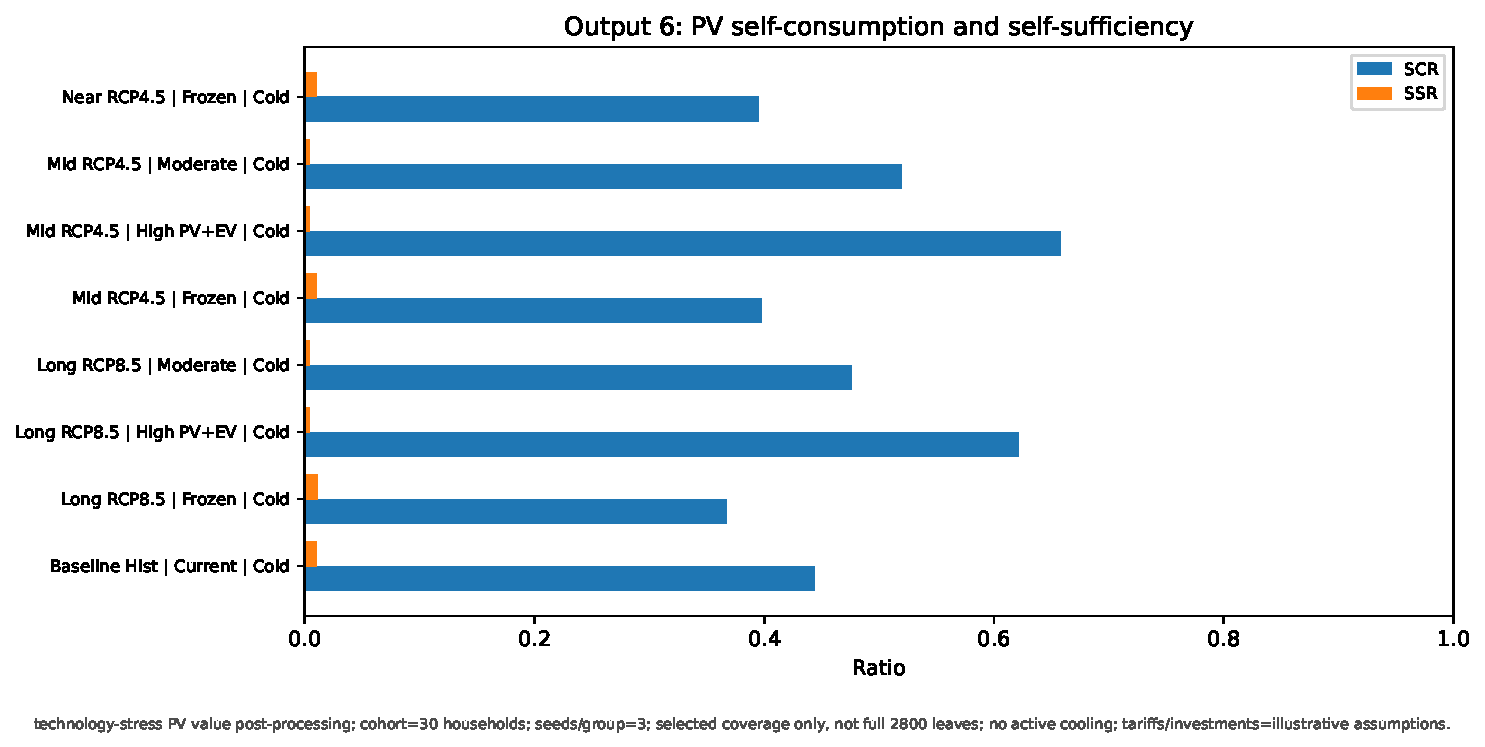
\includegraphics[width=0.9\textwidth]{figures/output6_pv_scr_ssr.pdf}
  \caption{PV self-consumption ratio and self-sufficiency ratio across executed technology cases.}
  \label{fig:pv_scr_ssr}
\end{figure}


\subsection{Residential Electrification}
%% Impact based on outputs of results chapter, good/bad, why, money-wise, etc. %%
The results complicate a simple pro-electrification interpretation. In the climate-only comparison, warming reduces heating pressure under a frozen residential stock: the long-term RCP\,8.5 case reduces HDD$_{18}$ by about \SI{31}{\percent} and useful-heating demand by about \SI{33}{\percent}. However, this physical reduction does not translate into a major reduction in residential grid stress, because the frozen-stock case remains largely gas-dominated. The hourly design-year results show that the dominant system change is instead the technology transition itself.

Under the executed long-term RCP\,8.5 cold-design-year case, frozen stock leaves peak grid import almost unchanged relative to the historical baseline, while moderate electrification raises the cohort peak to about \SI{87}{kW} and the high-electrification PV--EV case raises it to about \SI{184}{kW}. This means that residential electrification is not merely a fuel-substitution problem; it is also a coincidence and infrastructure problem. The modelled peak increase is much larger than the climate-only peak effect in the executed scenario subset.

The economic and emissions outputs point in the same direction of conditionality. Moderate electrification reduces operational emissions under the fixed electricity-emission factor, but it raises annual bills and annualized costs under the current tariff and CAPEX assumptions. The high-electrification PV--EV case performs worse in the current accounting: PV raises self-consumption, but the electrified load is large enough that grid import remains dominant, and operational emissions increase under the fixed-factor assumption. These results should not be read as evidence against electrification in general. Rather, they show that electrification is only beneficial under the right accompanying system conditions: lower-carbon electricity, sufficient network capacity, flexible heat-pump and EV operation, tariff structures that reward useful flexibility, and PV deployment that prioritises self-consumption rather than export.

The main discussion implication is therefore that electrification is a necessary decarbonisation pathway but not an automatically benign residential-demand pathway. In this model, unmanaged electrification shifts the residential challenge from annual heating demand toward peak power, coincidence, and tariff-sensitive affordability. The adaptation question is consequently not whether electrification occurs, but how it is coordinated with grid planning, cooling demand, PV self-consumption, and demand-side flexibility.



\subsection{From Stress to Strategy}
\label{sec:adaptation_summary}

Three implications follow from the executed results. First, climate forcing alone reduces heating demand and raises cooling pressure, but it does not materially increase the observed residential grid peak with the frozen stock. Electrification does: the hourly design-year results raise the cohort peak by roughly five to ten times relative to the historical current-stock baseline.

Second, cooling pressure is real in the indicator space but incomplete in the energy ledger. A future active-cooling module is needed before the model can quantify summer electricity demand, peak timing shifts, or the interaction between cooling load and PV generation.

Third, the economic and emissions results are conditional on tariff, export-credit, CAPEX, O\&M, and fixed electricity-emission assumptions. The defensible adaptation message is therefore about system shape rather than precise welfare ranking: electrification creates the dominant grid-stress channel; cooling-capable heat pumps become relevant because cooling pressure rises; and PV value depends increasingly on local absorption rather than export.

\begin{quote}\itshape
Under one CORDEX chain and the configured Belgian baseline, residential electrification is the dominant source of peak grid stress in the executed future design-year cases. Climate forcing alone is secondary for grid peak under the frozen stock, while rising cooling pressure and low-export PV economics make reversible heat-pump service and PV self-consumption the key adaptation directions to evaluate further.
\end{quote}


\pagebreak
\section{Limitations}\label{sec:limitations}

The limitations of this work are primarily ones of evidential scope. The model
supports comparison of internally consistent climate--technology scenarios, but
several components are not strong enough for national forecasting,
distribution-network design, or precise household-level prediction.


\subsection{Executed Scenario Coverage}
\label{sec:limitationsScenarioCoverage}

The scenario-tree design defines a far larger factorial space than was executed. The thesis evidence uses the completed subset in the canonical artefacts: 37 full-window climate/annual-demand leaves from \texttt{scenario\_tree/} and 48 hourly design-year leaves from \texttt{output34/}, i.e.\ 85 of the planned 2800 leaves.

The two sets answer different questions. The full-window runs drive the annual climate-pressure and heating-demand comparisons across climate windows and RCP pathways; the \texttt{output34} runs drive the hourly peak, diversity, bill, emissions, and adaptation diagnostics, but only for selected climate--technology combinations and a smaller cohort. The chapter accordingly makes no claim to full factorial coverage across pathway, window, technology case, design year, and seed.


\subsection{Climate Forcing Limitations}
\label{sec:limitationsClimateForcing}

The CORDEX forcing in the scenario tree is daily rather than hourly. Temperature and surface shortwave radiation are processed as daily variables, and the hourly
\texttt{output34} workflow forward-fills them to the model timestep. Hourly variation in those runs therefore arises from stochastic demand, occupancy, appliances, DHW, EV charging, PV profiles, and heating control, rather than from a reconstructed hourly future-weather signal.

Future-climate results are consequently most defensible at daily, seasonal, annual, and scenario-comparison scales, and should not be read as precise simulations of future hourly weather extremes, intra-day heat-wave dynamics, or sub-daily solar variability. The evidence also rests on a single CORDEX chain and a nearest-point extraction around the Belgian target location, rather than a multi-model ensemble or a spatially aggregated climate field; inter-GCM/RCM uncertainty, bias-correction uncertainty, and local urban or microclimate effects lie outside it.


\subsection{Demand Model \& Empirical Validation}
\label{sec:limitationsValidation}

The demand model combines archetype, stock, stochastic-use, and technology assumptions---appropriate for scenario exploration, but not equivalent to calibration against a large sample of measured Belgian household load curves. The clearest external warning is the Fluvius aggregate validation, where the representative-profile comparison currently fails: CVRMSE around 88\%, Pearson correlation around 0.40, annual-energy error around 56\%, and peak-timing error around 18 hours. This bounds any claim to reproduce observed Belgian aggregate electricity profiles.
\newline The remaining validation layers are more supportive but narrower. The Richardson-style comparison speaks to stochastic diversity structure rather than Belgian empirical accuracy; the KU\,Leuven high-frequency check covers only three houses and cannot provide statistical validation. PV validation is strong against PVGIS and Elia at physical and national-profile level but only moderate against the Fluvius residential PV signature. EV timing matches the Fluvius-derived signature well, while the base annual home-charging magnitude sits roughly 43\% below the reference---a gap the calibration sensitivity attributes to the annual-energy assumption rather than to timing.


\subsection{Cooling \& Comfort Scope}
\label{sec:limitationsCooling}

The model reports cooling pressure through indicators such as $\text{CDD}_{22}$, overheating exposure, indoor-temperature exceedance, and adaptation proxies, but the executed scenario-tree outputs contain no active cooling final electricity demand. The rise in cooling pressure under warmer scenarios is therefore visible as a climate and comfort signal that is not yet converted into summer electricity demand, cooling peak load, or cooling-related bills and emissions.

The reversible-heat-pump adaptation result should accordingly be read as a service and planning proxy: it shows that cooling-capable heat pumps gain relevance as heating demand falls and cooling pressure rises, without establishing a monetised investment optimum or simulating active cooling operation.


\subsection{Techno-Economic Limitations}
\label{sec:limitationsTechnoEconomic}

The technology cases are scenario assumptions rather than adoption forecasts. They support comparison of frozen-stock, moderate-electrification, and high-electrification futures, but do not model how households actually choose technologies, renovate, or adopt EVs and PV.
\newline Grid stress is captured through cohort-level grid-import peaks and threshold exceedance, with no distribution-network power-flow model. The results thus locate demand-side peak pressure without resolving transformer loading, voltage violations, cable congestion, protection constraints, or feeder-specific hosting capacity.

The bill figures are post-processing under configured tariff assumptions and are best read as illustrative tariff scenarios rather than Belgian tariff forecasts. The emissions figures are operational and factor-based: they apply fixed emission factors, exclude embodied emissions, omit time-varying marginal electricity factors, and give no export credit for displaced system emissions. These assumptions suffice for comparing directions within the model, but not for final policy-costing or lifecycle-carbon claims.


\subsection{Overall Interpretation Boundary}
\label{sec:limitationsInterpretationBoundary}

The model is strongest for comparing internally consistent scenario directions:
the reduction in heating pressure under warming, the dominance of electrification
in the hourly peak signal, the tariff sensitivity of household bills, and the
conditional nature of operational-emissions reductions. It is weaker as a source
of absolute national figures, and the results are best read as a structured
scenario experiment for Belgian residential demand rather than a calibrated
national energy-system forecast.


\pagebreak
\section{Future Work}\label{sec:futurework}

Future work should focus on turning the present scenario framework into a more
complete empirical and operational platform, prioritising the gaps identified in
\Cref{sec:limitations}.


\subsection{Scenario Tree Broadening}
\label{sec:futureworkScenarioTree}

The first priority is to execute a larger and more balanced share of the planned
tree, extending the hourly \texttt{output34} workflow beyond the selected
design-year and technology combinations so that uncertainty bands can be
reported across climate windows, pathways, technology cases, seeds, and design
years. This also requires a formal link between the full-window annual runs and
the hourly design-year runs---either hourly simulation over longer windows, or a
documented sampling strategy that maps each annual climate window to
representative hourly design years.


\subsection{Climate Forcing \& Cooling Modelling}
\label{sec:futureworkClimateCooling}

The climate pipeline should move from a single CORDEX chain to a multi-model
ensemble, and from a nearest-point extraction to spatial aggregation over
Belgium, so that results report spread across GCM/RCM combinations rather than
one realisation. The hourly treatment of future weather should likewise replace
the forward-filled daily forcing with a documented temporal downscaling of
temperature and solar radiation, or with bias-corrected hourly climate
products---most important for peak-load, cooling, PV, and heat-pump questions.
Cooling should then be implemented as an explicit end use, converting the
present cooling-pressure indicators into summer electricity demand, peak
contribution, comfort, bills, and emissions, which would also make the
reversible-heat-pump adaptation analysis operational.


\subsection{Empirical Validation}
\label{sec:futureworkValidation}

The priority for validation is measured Belgian household or feeder-level
electricity data at sufficient temporal resolution. The failing Fluvius
aggregate comparison should be treated as an open model-development issue and
diagnosed against its likely causes: annual magnitude, appliance profiles,
heating-electrification assumptions, occupancy schedules, profile alignment, or
reference representativeness. Each validation purpose---end-use calibration,
diversity structure, aggregate load shape, PV, EV, and high-frequency event
realism---should also carry its own acceptance criteria, so that strength in one
layer is not overread as validation of another.


\subsection{Electrification \& Flexibility}
\label{sec:futureworkElectrification}

The electrification scenarios should gain an explicit flexibility layer.
Heat-pump preheating, thermal storage, EV smart charging, PV self-consumption,
and tariff-responsive operation are currently represented only partly or through
post-processing sensitivities, and a physical dispatch or control layer would
test whether the large electrification peaks can be reduced without unacceptable
comfort, cost, or emissions penalties. The technology stock should also be tied
to renovation pathways and adoption constraints---heat-pump suitability by
envelope quality, emitter temperature, dwelling type, ownership, and renovation
state---making the scenarios less stylised and more policy-relevant.


\subsection{Distribution-Network \& System Coupling}
\label{sec:futureworkGrid}

The cohort-level import metrics should be connected to a low- or medium-voltage
network model, allowing transformer loading, feeder congestion, voltage
deviations, and hosting capacity to be assessed directly rather than inferred
from demand-side peaks. Coupling the household model to system-level
assumptions---time-varying marginal emission factors, dynamic wholesale prices,
renewable availability, and grid constraints---would further improve the bill
and emissions results, particularly for PV, EV charging, and heat-pump
operation.


\subsection{Economic \& Emissions Accounting}
\label{sec:futureworkEconomicsEmissions}

The bill model should adopt more detailed Belgian tariff structures (supplier
contracts, capacity tariffs, taxes and levies, injection compensation, regional
differences), and the investment layer should move beyond illustrative CAPEX and
O\&M assumptions toward explicit retrofit costs, lifetimes, discount rates, and
affordability constraints. The emissions model should replace fixed operational
factors with time-varying, scenario-dependent ones and, where the scope extends
to lifecycle impact, include embodied emissions for PV, batteries, heat pumps,
EVs, and renovation measures. Exported PV should be accounted for consistently,
whether on a household-boundary or a system-displacement basis.


\subsection{Reproducibility \& Benchmarking}
\label{sec:futureworkReproducibility}

Finally, the manifest-based provenance already attached to each
\texttt{scenario\_leaf\_id} should be extended with automated regression tests on
the headline thesis metrics, so that changes in code, input data, or assumptions
surface as changes in the reported results. This would support both academic
audit and comparison with other residential-demand models.

% Future work should focus on converting the present scenario framework into a more complete empirical and operational modelling platform. 


% \subsection{Complete and Broaden the Scenario Tree}
% \label{sec:futurework_scenario_tree}

% The first priority is to complete a larger share of the planned scenario tree and to make the executed subset more balanced. In particular, the hourly \texttt{output34} workflow should be extended beyond the selected design-year and technology combinations used in this thesis. A fuller run matrix would allow uncertainty bands across climate windows, pathways, technology cases, stochastic seeds, and design years, instead of relying on selected contrasts.

% A second priority is to standardise the connection between the full-window annual runs and the hourly design-year runs. At present, the former are best suited to annual climate-pressure interpretation, while the latter are best suited to peak and techno-economic interpretation. Future work should either run hourly simulations over longer climate windows or define a formal sampling strategy that maps annual climate windows to representative hourly design years.


% \subsection{Improve Climate Forcing and Cooling Modelling}
% \label{sec:futurework_climate_cooling}

% The climate pipeline should be extended from a single CORDEX chain to a multi-model ensemble. This would allow the thesis-style results to report spread across GCM/RCM combinations rather than only one climate realisation. Spatial aggregation over Belgium or over representative Belgian regions would also be preferable to a single nearest-point extraction when making national statements.

% The hourly treatment of future weather should also be improved. Rather than forward-filling daily CORDEX variables to hourly timesteps, future work could apply a documented temporal downscaling method for temperature and solar radiation, or couple the model to bias-corrected hourly climate products where available. This is especially important for peak-load, cooling, PV, and heat-pump performance questions.

% Active cooling should be implemented as an explicit end use. The current model can identify rising cooling pressure, but future work should convert that pressure into cooling electricity demand, summer peak contribution, indoor comfort improvement, bill impacts, and emissions impacts. This would make the reversible-heat-pump adaptation analysis more operational.


% \subsection{Strengthen Empirical Validation}
% \label{sec:futurework_validation}

% The most important validation extension is measured Belgian household or feeder-level electricity data with sufficient temporal resolution and metadata. The current Fluvius aggregate validation fails and should be treated as an open model-development issue. Future work should diagnose whether the failure comes from annual magnitude, appliance profiles, heating electrification assumptions, occupancy schedules, profile alignment, or the representativeness of the reference data.

% Validation should also be separated more sharply by purpose. End-use calibration, stochastic diversity validation, aggregate load-shape validation, PV validation, EV validation, and high-frequency event realism should each have their own acceptance criteria. This would prevent supportive evidence in one layer from being overread as validation of another layer.


% \subsection{Extend Electrification and Flexibility Modelling}
% \label{sec:futurework_electrification}

% The electrification scenarios should be expanded with explicit flexibility. Heat-pump preheating, thermal storage, EV smart charging, PV self-consumption control, and tariff-responsive operation are currently represented only partly or through post-processing sensitivities. A physical dispatch or control layer would allow the model to test whether the large peak increases observed under electrification can be reduced without unacceptable comfort, cost, or emissions penalties.

% The technology stock model should also be linked more directly to renovation pathways and adoption constraints. Future work could distinguish heat-pump suitability by envelope quality, emitter temperature, dwelling type, ownership status, and renovation state. This would make the electrification scenarios less stylised and more useful for policy interpretation.


% \subsection{Add Distribution-Network and System Coupling}
% \label{sec:futurework_grid}

% The present grid-stress indicators are cohort-level import metrics. Future work should connect the residential demand outputs to a low-voltage or medium-voltage network model. This would allow transformer loading, feeder congestion, voltage deviations, and hosting capacity to be assessed directly.

% A further extension would couple the household model to system-level electricity assumptions. Time-varying marginal emission factors, dynamic wholesale prices, renewable availability, and grid constraints would make the bill and emissions results more realistic, especially for PV, EV charging, and heat-pump operation.


% \subsection{Refine Economic and Emissions Accounting}
% \label{sec:futurework_economics_emissions}

% The bill model should be updated with more detailed Belgian tariff structures, including supplier contracts, capacity-tariff implementation, taxes, levies, injection compensation, and regional differences. The investment layer should also move beyond illustrative CAPEX and O\&M assumptions toward explicit retrofit costs, equipment lifetimes, discount rates, replacement cycles, and household affordability constraints.

% The emissions model should be extended from fixed operational factors to time-varying and scenario-dependent electricity factors. Embodied emissions for PV, batteries, heat pumps, EVs, and renovation measures should be included if the research question is expanded from operational demand to lifecycle climate impact. Exported PV should also be treated consistently, either as household-boundary accounting or as system-displacement accounting, but not left implicit.


% \subsection{Reproducibility and Benchmarking}
% \label{sec:futurework_reproducibility}

% The manifest-based reproducibility structure is a useful base and should be kept. Future work should add automated regression tests for the headline thesis metrics, so that changes in code, input data, or assumptions automatically flag changes in the reported results. A public benchmark package containing selected configs, input hashes, output summaries, and validation scripts would make the model easier to audit and compare with other residential-demand models.

% The long-term goal should be a model that can report not only one set of scenario outcomes, but also the uncertainty and validation status attached to each claim. That would make the framework more useful for both academic review and policy-facing interpretation.

% \section{Model v1}
% %%% BASELINE %%%
% %%% discuss sec:futurework & gaps %%%

% A link to the GitHub repository of the entire pipeline of the first model can be found \href{https://github.com/LexTS1/ED_thesis_model-v1.git}{here}.
% \newline The unified \textit{Model v1} represents an important integration step in this thesis, because it brings the data layer, the physics modules, the control logic, and the output generation into one reproducible pipeline. This model's main contribution is therefore architectural rather than conceptual: it composes the previously developed modules into a single workflow without duplicating earlier code. This composition is orchestrated primarily in \textit{run\_model\_v1.py}, through the functions \hyperref[lst:v1-pipeline-run]{run\_model\_v1()} and \hyperref[lst:v1-pipeline-execute]{\_execute\_model\_v1()}, which call the existing modules from versions v1.2 to v1.5 in sequence.

% \subsection{Limitations}
% The structure of \textit{Model v1} is strong from a software-engineering perspective, but it inherits many of the assumptions, simplifications, and boundary conditions of the earlier versions (v1.1--v1.5). As a result, the unified model should be interpreted as a coherent synthesis of the existing framework, not yet as a fully mature or fully validated residential energy-demand model.

% \subsubsection*{Limited scope}
% A first limitation is the scope of representation. In its current form, \textit{Model v1} still behaves essentially as a dwelling-scale or archetype-scale model rather than as a calibrated building-stock model. The unified execution path in \textit{run\_model\_v1.py} produces a single model trajectory for one selected archetype and one set of household assumptions. The archetype itself is resolved through \hyperref[lst:v1-archetype-resolve]{resolve\_selected\_archetype()} in \textit{archetype\_parameters.py} from v1.4 and v1.5, while occupancy is scaled through \hyperref[lst:v1-occupancy-expected]{build\_expected\_occupancy()} in \textit{occupancy.py} and integrated in \textcolor{gray}{prepare\_model\_ready\_inputs()} in \textit{adapters.py}. This makes the model suitable for tracing causal relationships between weather, gains, airflow, control, and energy demand, but it limits its representativeness at aggregate level. In particular, household diversity, heterogeneity in building quality, differences in occupant behaviour, and variation in system performance are not yet represented explicitly as a population. Consequently, aggregate comparisons with benchmark or smart-meter datasets should be understood as plausibility checks rather than proof of stock-level accuracy.

% \subsubsection*{Electrical Output}
% A second limitation concerns the semantics of the electrical output. The unified pipeline computes internal gains from occupancy, appliances, lighting, and cooking through \hyperref[lst:v1-internal-gains]{compute\_internal\_gains()} in \textit{internal\_gains.py}, and these quantities are assembled into the final output table through \textcolor{gray}{\_build\_output\_frame()} in \textit{run\_model\_v1.py}. However, the electrical output itself is still computed by \hyperref[lst:v1-electricity-demand]{compute\_electricity\_demand()} in \textit{electricity\_model.py}, where P\_el\_W is derived only from q\_heat\_w, q\_dhw\_w, and cop. In other words, several non-thermal end uses are represented more clearly as internal heat gains than as explicit electrical end uses. This weakens the interpretation of the electricity results, especially when the model is compared against empirical household electricity measurements in the validation layer. For a truly comparable total-demand model, future versions should distinguish explicitly between thermal demand, thermal-system electricity, and direct end-use electricity, and should report these components separately before aggregation.

% \subsubsection*{System layer distinction}
% A third limitation lies in the simplification of the control and system layer. The thermostat logic is intentionally simple, relying on \hyperref[lst:v1-control-deadband]{compute\_deadband\_heating()} in \textit{heating\_control.py}, together with \hyperref[lst:v1-control-setpoint-schedule]{build\_setpoint\_schedule()} in \textit{setpoint\_schedule.py}. In the unified pipeline, these are called in \textit{run\_model\_v1.py}, after which indoor temperature is updated by \textit{dynamic\_temperature.py}. This is sufficient to test the interaction between occupancy schedules, gains, temperature evolution, and heating demand, but it does not yet capture several behaviours that matter in real buildings and real heating systems. Examples include plant capacity constraints, emitter dynamics, control delays, cycling behaviour, part-load efficiency effects, and explicit unmet demand. In addition, the current comfort-cap handling is implemented through \hyperref[lst:v1-control-temperature-limits]{apply\_temperature\_limits()} in \textit{temperature\_limits.py}, which is applied after the thermal state update in \textit{run\_model\_v1.py}. This is operationally useful, but not yet fully energy-consistent, because temperature limiting is applied as a post-processing constraint on the thermal state rather than as an explicit physical process with a corresponding energy term. This means that thermal realism is improved in a numerical sense, but not yet closed rigorously in an energy-balance sense.

% \subsubsection*{Data and preprocessing}
% A fourth limitation concerns the data and preprocessing layer. The inclusion of a shared missing-data and uncertainty module is a major improvement over earlier isolated workflows, because it makes data treatment explicit and reproducible. Input loading is handled by \textit{load\_inputs.py}, where the individual sources are normalized and merged. Preprocessing is then handled in \textit{preprocess\_inputs.py}, which delegates missing-data operations to the shared functions \textcolor{gray}{detect\_missing()} in \textit{detect\_missing.py}, \textcolor{gray}{classify\_gaps()} in \textit{classify\_gaps.py}, and \textcolor{gray}{reconstruct\_timeseries()} in \textit{reconstruct\_timeseries.py}. Stochastic propagation is introduced later through \textcolor{gray}{generate\_stochastic\_datasets()} in \textit{uncertainty\_model.py}, called from \hyperref[lst:v1-pipeline-stochastic]{run\_model\_v1\_stochastic()} in \textit{run\_model\_v1\_stochastic.py}. However, uncertainty propagation currently remains narrow in scope. It is mainly applied to reconstructed input values, while other important uncertainties are held fixed, such as archetype parameters, occupancy behaviour, ventilation behaviour, thermostat preferences, and system performance. Furthermore, when multiple sources with different temporal resolutions are merged in \textit{load\_inputs.py}, part of the difficulty becomes one of alignment and structural sparsity rather than purely random missingness. This means that the preprocessing layer is robust for controlled reconstruction, but it should not yet be interpreted as a full probabilistic treatment of input uncertainty.

% \subsubsection*{Limited validation}
% A fifth limitation concerns validation. The unified pipeline correctly keeps validation separate from the runtime model, which is methodologically appropriate. Nevertheless, the current validation evidence remains uneven across domains. The electricity validation against Richardson-type synthetic benchmarks and smart-meter data provides useful behavioural checks, but only moderate agreement should be expected given the simplified dwelling representation and the remaining ambiguity in electrical end-use accounting. The thermal validation is also informative, but it remains more directional than direct, because the Fischer workflow implemented in \textit{validate\_fischer.py} does not yet compare against a measured thermal truth series. As a result, the present validation framework is best understood as layered evidence of plausibility rather than definitive confirmation of predictive accuracy.

% \subsection{Interpretation}
% These limitations do not diminish the value of \textit{Model v1}; rather, they clarify its role in the thesis. \textit{Model v1} should be seen as a stable integration baseline: it unifies the previously separate developments, makes assumptions more transparent, and creates a practical platform for systematic extension. In software terms, this baseline is mainly defined by the orchestration scripts \textit{run\_model\_v1.py}, \textit{run\_model\_v1\_stochastic.py}, \textit{load\_inputs.py}, \textit{preprocess\_inputs.py}, and \textit{adapters.py}. The main gap for a future \textit{Model v2} is therefore not simply ``more detail'', but improved model meaning and improved comparability. In particular, a next version should introduce explicit end-use electricity accounting, energy-consistent comfort and control constraints, richer household and archetype diversity, broader uncertainty propagation, and stronger empirical validation against directly comparable measured quantities.


% \section{Model v3}
%%% GUI + application & deployment %%%
%%% discuss improvements, limitations & gaps %%%

\mode<all> % do not remove
    \chapterOrPart{Conclusions}\label{ch:conclusions}

\begin{explanation}
    This chapter is mandatory. Your work must have conclusions.
    
    The conclusions contain your main findings and the answer to the research question(s) in a clear and concise way. Conclusions should not contain results that have not yet been discussed in your work.
\end{explanation}

The central answer is that climate forcing and technology-stock assumptions interact asymmetrically in the executed thesis model. Under a frozen technology stock, climate forcing mainly changes the useful thermal side of the residential balance: in the strongest reported case, long-term RCP\,8.5, HDD$_{18}$ falls by about \SI{31.0}{\percent}, CDD$_{22}$ rises by about $94.9\,^{\circ}\mathrm{C}\cdot\mathrm{d}$ per year, and useful space-heating demand falls by about \SI{33.3}{\percent}. This answers the first supporting question: warming reduces heating pressure and raises cooling pressure, but the current model does not convert cooling pressure into active cooling electricity demand. Climate forcing alone therefore changes annual heating indicators much more clearly than it changes peak grid import under the frozen stock; in the cold-design-year comparison, the peak remains essentially unchanged at about \SI{30.6}{kW} versus the historical \SI{30.8}{kW}.

The technology cases dominate the final-energy carrier and peak-load results. In the cold-design-year long-term RCP\,8.5 comparison, frozen stock reduces gas use while leaving peak import close to the historical baseline, but moderate electrification raises cohort peak import to about \SI{106.45}{kW}, and the high-electrification PV--EV case raises it to about \SI{188.40}{kW}. This answers the second supporting question: electrification shifts residential demand from fossil carriers toward electricity and strongly increases grid-import stress when unmanaged, while PV affects self-consumption and export but does not remove the peak problem in the executed high-electrification case. The economic and emissions results are conditional on the configured tariff, CAPEX and fixed emission-factor assumptions: frozen stock lowers the dynamic-tariff bill and operational emissions, moderate electrification lowers operational emissions only slightly while raising bills, and the high-electrification PV--EV case raises both bills and operational emissions under the fixed-factor accounting.

The stochastic and validation evidence set the interpretation boundary for the whole thesis. Household diversity is represented through stochastic cohorts and the Richardson-style validation indicates plausible diversity structure, but the executed design-year results use five stochastic seeds and do not provide a full variance decomposition across climate, technology and behaviour. The third supporting question is therefore only partially answered: technology-driven peak differences are visibly much larger than the frozen-stock climate-only peak effect in the reported stress table, but the thesis should not claim a fully quantified stochastic uncertainty hierarchy. The fourth supporting question is also mixed. Annual calibration converges, PV validation is strong against PVGIS and Elia, and EV timing agrees well with the Fluvius EV signature, but the aggregate Fluvius smart-meter profile comparison fails with CVRMSE around \SI{88}{\percent}, Pearson correlation around $0.40$, and peak-timing error around $18$ hours. The model is consequently defensible as a traceable conditional scenario model for Belgian residential demand, not as an externally calibrated Belgian smart-meter forecasting model.


\mode<all> % do not remove

    %\chapterOrPart{Future Work}\label{ch:futurework}

\begin{explanation}
    It is common practice to formulate future work in a thesis. But it must not necessarily be done in a separate chapter. It can also be a section in the chapter with conclusions.
\end{explanation}

\mode<all> % do not remove
\appendix
    \chapterOrPart{Source Codes}\label{ch:scripts}

Because including the full repository source code would exceed a reasonable page count, only the canonical model configuration are reproduced here. The original source code can be found at the final \href{https://github.com/LexTS1/ED_thesis_model-v3.git}{GitHub} repository.

\begin{lstlisting}[caption={Canonical model configuration (\texttt{config/thesis.yaml})}, label={lst:modelConfig}]
modules:
  physics: true
  control: true
  systems: true
  cohort: true
  stochastic: true

technology_inputs_path: "belgian_technology_inputs.yaml"

simulation:
  n_samples: 2
  start_timestamp: "2023-01-01T00:00:00+01:00"
  reference_year: 2023
  max_steps: ~

baseline:
  electricity_annual_kWh: 3500
  electricity_range_kWh: [3000, 3900]
  space_heating_kWh: 12000
  space_heating_range_kWh: [12000, 16000]
  dhw_kWh: 3000
  dhw_range_kWh: [2500, 3300]

electricity_split:
  appliances: 0.70
  lighting: 0.08
  cooking: 0.10
  dhw: 0.07
  space_heating: 0.05
  other: 0.0
  note: >
    Central electricity target is aligned to the common Belgian standard-household
    benchmark of 3500 kWh/year. Thermal services are primarily represented through
    useful heat and carrier conversion; the DHW and space-heating electricity
    shares are retained as modest auxiliary/direct-electric current-stock
    components rather than dominant electric heating loads.

thermal_split:
  space_heating: 0.83
  dhw: 0.17

technology_baseline:
  gas_share: 0.49
  oil_share: 0.39
  electric_share: 0.07
  other_share: 0.05
  heat_pump_share: 0.04

heat_pump:
  cop_nominal_range: [3.0, 5.0]
  note: "Use as nominal; apply seasonal degradation"

cohort:
  n_households: 30
  minimum_households: 30
  random_seed: 42
  diversity_slots: 24
  quantile_buffer_size: 512

climate:
  enabled: false
  mode: "climate_only"
  n_members: 50
  seed: 42
  rho: 0.8
  occupancy_seed: 42
  occupancy_seed_stride: 1000
  mu_month: {}
  inputs:
    weather_path: "inputs/weather/Timeseries_pvgisWEATHER_50.830_4.350_SA3_0deg_0deg_2005_2023.csv"
    solar_paths:
      south: "inputs/solar/TimeseriesSOUTH_50.830_4.350_SA3_90deg_0deg_2005_2023.csv"
      east: "inputs/solar/TimeseriesEAST_50.830_4.350_SA3_90deg_-90deg_2005_2023.csv"
      west: "inputs/solar/TimeseriesWEST_50.830_4.350_SA3_90deg_90deg_2005_2023.csv"
      north: "inputs/solar/TimeseriesNORTH_50.830_4.350_SA3_90deg_-179deg_2005_2023.csv"

uncertainty:
  physical:
    sample_building_archetype_by_stock_weight: true
    UA_sigma: 0.25
    thermal_mass_sigma: 0.20
    infiltration_sigma: 0.4
    cop_sigma: 0.10
  behaviour:
    occupancy_sigma: 0.2
    dhw_sigma: 0.4
    dhw_cohort_scale: 3.217
    dhw_calibration:
      enabled: true
      daily_useful_kWh_per_person:
        low: 0.8
        base: 1.2
        high: 1.5
      equivalent_litres_per_person_day_42C:
        base: 32.0
      cold_water_temperature_C: 10.0
      draw_temperature_C: 42.0
      event_frequency_per_occupant_day:
        low: 1.4
        base: 2.0
        high: 3.0
      timing_weights:
        morning:
          start_hour: 6.0
          end_hour: 9.0
          weight: 0.45
        daytime:
          start_hour: 9.0
          end_hour: 18.0
          weight: 0.12
        evening:
          start_hour: 18.0
          end_hour: 22.0
          weight: 0.40
        night:
          start_hour: 22.0
          end_hour: 6.0
          weight: 0.03
      event_type_probabilities:
        sink: 0.58
        shower: 0.26
        dishwashing: 0.13
        bath: 0.03
      event_volume_liters:
        sink:
          low: 1.0
          high: 6.0
        shower:
          low: 25.0
          high: 65.0
        dishwashing:
          low: 8.0
          high: 18.0
        bath:
          low: 80.0
          high: 140.0
      source_note: "Bounded useful draw-off DHW calibration from Belgian/European residential water-use and DHW profile literature; production/storage/distribution losses remain outside Q_dhw_demand_W."
    appliance_sigma: 0.5
    household_size_probabilities:
      1: 0.36
      2: 0.31
      3: 0.145
      4: 0.11
      5: 0.04
      6: 0.02
      7: 0.01
    household_size_distribution_note: "Belgian private-household-size working distribution; normalized during sampling because rounded probabilities sum to 0.995."
    dhw_event_volume_sigma: 0.4
    dhw_event_lambda: 3.0
    dhw_start_jitter_hours: 0.75
    appliance_start_jitter_hours: 1.0
    high_frequency_sigma: 0.08
  technology:
    use_belgian_stock_baseline: true
    heat_pump_share: 0.6
    resistive_share: 0.4

data:
  target_resolution_seconds: 3600
  harmonisation:
    methods:
      weather: forward_fill
      load_profiles: mean
      internal_gains: mean
      solar: mean
  reconstruction:
    methods:
      weather: forward_fill
      load_profiles: zero_fill
      internal_gains: zero_fill
      solar: zero_fill
  sources:
    occupancy:
      spec_path: "inputs/occupancy/occupancy_model_spec_v1.yaml"
      data_role: ["input"]
    weather:
      file_path: "inputs/weather/aws_1hour_Uccle.csv"
      data_role: ["input"]
      timestamp_column: "timestamp"
      column_mapping:
        T_outdoor_C: "temp_dry_shelter_avg"
      original_timestep_seconds: 3600
      timestamps:
        - "2023-01-01T00:00:00+01:00"
      data:
        T_outdoor_C: [5.0]
    load_profiles:
      file_path: "inputs/load_profiles/LCL_2013.csv"
      data_role: ["input"]
      timestamp_column: "DateTime"
      original_timestep_seconds: 1800
      units: "kWh_per_interval"
      timestamps:
        - "2023-01-01T00:00:00+01:00"
      data:
        appliances: [0.0]
        lighting: [0.0]
        cooking: [0.0]
    end_use_shares:
      file_path: "inputs/end_use/EU27_BE_household_enduse_2019.csv"
      data_role: ["calibration"]
      parameter_column: "parameter"
      value_column: "value"
      lighting_fraction_of_appliance_bucket: 0.18
    internal_gains:
      data_role: ["input"]
      original_timestep_seconds: 3600
      timestamps:
        - "2023-01-01T00:00:00+01:00"
      data:
        Q_internal_gains_W: [0.0]
    solar:
      raw_dir: "inputs/solar/raw_inputs"
      data_role: ["input"]
      original_timestep_seconds: 3600
      timestamps:
        - "2023-03-15T13:00:00+01:00"
      data:
        Q_solar_gains_W: [0.0]

forcing:
  T_outdoor_C: 5.0
  T_indoor_initial_C: 17.0
  T_set_C: 21.0
  dhw:
    demand_W: 0.0
  electric_loads_W:
    appliances: 0.0
    lighting: 0.0
    cooking: 0.0

building:
  heat_loss_coefficient_W_per_C: 180.0
  ua_multiplier: 0.80
  ua_calibration_note: >
    Explicit thesis thermal calibration factor. The value 0.80 was selected
    from full-horizon 2023 baseline validation to align useful space-heating
    demand with the configured Belgian literature range while leaving annual
    electricity and DHW calibration unchanged. Treat this as baseline thermal
    calibration, not as an independently observed envelope parameter.
  thermal_mass_Wh_per_C: 4500.0
  tabula_archetypes_path: "config/archetypes.yaml"
  archetype_source:
    file_path: "inputs/building/archetype_parameters_merged_v3.csv"
    selection: "stock_weighted_average"
  internal_gains_reference_csv: "inputs/building/internal_gains_archetypes_v2.csv"
  airflow_reference_csv: "inputs/building/airflow_archetypes_v2.csv"

model:
  timestep_seconds: 3600
  initial_indoor_temperature_C: 17.0
  occupancy_threshold: 0.5
  initial_heating_on: false

control:
  deadband: 1.0

setpoints:
  occupied_day: 21.0
  sleeping: 17.0
  away: 16.0

air:
  rho: 1.2
  cp: 1000.0

ventilation:
  window_opening:
    enabled: false
    extra_ach: 0.5
    trigger_above_setpoint_c: 1.0
    min_indoor_minus_outdoor_c: 1.0

systems:
  heating:
    capacity_W: 8000
    cop: 3.0
    ground_source_temperature_C:
      low: 4.0
      base: 8.0
      high: 12.0
      unit: degC
      source_note: "Category I/II shallow geothermal assumption; Belgian ground temperature around 10-14C at 20-30m, adjusted downward for entering brine/source temperature."
  dhw:
    cop: 1.0
  heat_pump_performance:
    types:
      air_water:
        cop_ref: 4.4
        min_cop: 2.0
        max_cop: 5.0
        defrost_penalty_fraction: 0.12
      air_air:
        cop_ref: 4.4
        min_cop: 2.0
        max_cop: 5.3
        defrost_penalty_fraction: 0.12
      ground_source:
        cop_ref: 3.8
        min_cop: 3.0
        max_cop: 5.2

comfort:
  T_min_C: 18
  T_max_C: 26

outputs:
  root_dir: "outputs"

validation:
  enabled: true
  dataset: "fluvius_external"
  model_source: "cohort"
  aggregate_mode: "fluvius_external"
  resolution: "auto"
  quick_mode:
    enabled: false
    max_steps: 168
    cohort_households: 5
    minimum_households: 5
  fluvius:
    enabled: true
    base_path: "inputs/load_profiles/fluvius"
    households: 30
    pv_variant_policy: "no_pv_only"
    model_value_column: "P_el_gross_actual_W"
    profile_weights:
      base: 0.9583
      ev: 0.0136
      hp: 0.0277
      ev_hp: 0.0004
  synthetic:
    acceptance:
      monthly_MBE_max: 0.05
      monthly_CVRMSE_max: 0.15
      hourly_MBE_max: 0.10
      hourly_CVRMSE_max: 0.50
      peak_MAE_kW_max: 2.0
      quantile_error_kW_max: 1.0
      good_hourly_MBE_max: 0.05
      good_hourly_CVRMSE_max: 0.30
      good_peak_MAE_kW_max: 1.0
      good_quantile_error_kW_max: 0.5
  kuleuven:
    enabled: true
    base_path: "inputs/load_profiles/kul"
    model_value_column: "P_el_gross_actual_W"
    cache_dir: "outputs/validation/cache/kuleuven_high_freq"
    quick_max_file_mb: 100.0
  aggregate_reference_year_mode: "map_to_model_year"
  timestamp_column: "DateTime"
  aggregate_aggregation: "mean_across_columns"
  aggregate_units: "kWh_per_interval"
  aggregate_interval_seconds: 1800
  acceptance:
    monthly_MBE_max: 0.05
    monthly_CVRMSE_max: 0.15
    hourly_MBE_max: 0.10
    hourly_CVRMSE_max: 0.30
    peak_MAE_kW_max: 0.2
    quantile_error_kW_max: 0.2
    good_hourly_MBE_max: 0.05
    good_hourly_CVRMSE_max: 0.20
    good_peak_MAE_kW_max: 0.1
    good_quantile_error_kW_max: 0.1
\end{lstlisting}

% \section{Scripts v1}

% \subsection*{Pipeline Orchestration}

% \begin{lstlisting}[
% caption={Core deterministic execution routine of Model v1 from run\_model\_v1.py.},
% label={lst:v1-pipeline-execute}
% ]
% def _execute_model_v1(
%     config_path: str | Path,
%     config: dict[str, Any],
%     raw_input_dataset: RawInputDataset,
%     preprocessed_inputs: PreprocessedInputs,
%     write_outputs: bool,
%     diagnostics_enabled: bool,
%     diagnostics_json_path: str | Path | None,
%     figures_dir: str | Path | None,
% ) -> dict[str, Any]:
%     model_inputs = prepare_model_ready_inputs(
%         cleaned_dataset=preprocessed_inputs.cleaned_dataset,
%         raw_input_dataset=raw_input_dataset,
%         config=config,
%     )
%     building_context = resolve_building_context(
%         building_cfg=dict(config["building"]),
%         solar_cfg=dict(config["solar"]),
%     )
%     internal_gains, internal_metadata = compute_internal_gains(
%         timestamps=model_inputs.frame["timestamp"],
%         occupancy_spec=model_inputs.occupancy_spec,
%         occupants_per_dwelling=float(config["building"]["occupants_per_dwelling"]),
%         gains_cfg=dict(config["internal_gains"]),
%         input_frame=model_inputs.frame,
%         floor_area_m2=building_context["floor_area_m2"],
%     )
%     solar_gains, solar_parameter_table = compute_solar_gains(
%         timestamps=model_inputs.frame["timestamp"],
%         solar_cfg=dict(config["solar"]),
%         building_cfg=dict(config["building"]),
%         timezone_name=str(config.get("timezone") or "Europe/Brussels"),
%         irradiance_frame=model_inputs.irradiance_frame,
%         solar_inputs_cfg=dict(config.get("inputs", {}).get("irradiance") or {}),
%     )
%     archetype_v1_4 = resolve_v1_4_archetype(config["archetypes"])
%     static_heat_balance = compute_heat_balance_v1_3(
%         t_out_c=model_inputs.frame["T_out_C"],
%         ua_w_per_k=archetype_v1_4.ua_w_per_k,
%         t_set_c=archetype_v1_4.t_set_c,
%         q_internal_w=internal_gains["Q_internal_total_W"],
%         q_solar_w=solar_gains["Q_solar_W"],
%     )
%     dynamic_output = _run_controlled_dynamics(
%         model_inputs=model_inputs,
%         config=config,
%         q_internal_w=internal_gains["Q_internal_total_W"],
%         q_solar_w=solar_gains["Q_solar_W"],
%     )

%     cop = pd.Series(
%         compute_cop_from_config(
%             t_out_c=model_inputs.frame["T_out_C"].to_numpy(dtype=float),
%             systems_cfg=dict(config["systems"]),
%         ),
%         name="COP",
%     )
%     dhw_output = compute_dhw_from_config(
%         timestamps=model_inputs.frame["timestamp"],
%         expected_occupants=model_inputs.frame["expected_occupants"],
%         occupied_probability=model_inputs.frame["occupied_probability"],
%         dhw_cfg=dict(config["dhw"]),
%     )
%     electricity_output = compute_electricity_demand(
%         q_heat_w=dynamic_output["Q_heat_W"],
%         q_dhw_w=dhw_output["Q_DHW_W"],
%         cop=cop,
%         dhw_cop=float(config["systems"].get("dhw_cop", 1.0)),
%     )
%     model_output = _build_output_frame(
%         model_inputs=model_inputs,
%         internal_gains=internal_gains,
%         solar_gains=solar_gains,
%         static_heat_balance=static_heat_balance,
%         dhw_output=dhw_output,
%         dynamic_output=dynamic_output,
%         electricity_output=electricity_output,
%         cop=cop,
%     )
%     model_output.attrs["internal_gains_metadata"] = internal_metadata
%     model_output.attrs["solar_parameter_table"] = solar_parameter_table.to_dict(orient="records")

%     output_paths: dict[str, str] | None = None
%     if write_outputs:
%         model_output_path = ensure_parent(config["outputs"]["model_output_parquet"])
%         model_output.to_parquet(model_output_path, engine=parquet_engine(), index=False)
%         output_paths = {"model_output_parquet": str(model_output_path.resolve())}

%     diagnostics = {}
%     if diagnostics_enabled and figures_dir is not None:
%         diagnostics = generate_diagnostics_model_v1(
%             model_output=model_output,
%             preprocessing_metadata=preprocessed_inputs.metadata,
%             figures_dir=figures_dir,
%             diagnostics_json_path=diagnostics_json_path,
%         )
%         if write_outputs and output_paths is not None:
%             output_paths["diagnostics_json"] = str(resolve_repo_path(diagnostics_json_path).resolve()) if diagnostics_json_path else None

%     summary = _summarize_run(
%         config_path=config_path,
%         config=config,
%         model_output=model_output,
%         preprocessing_metadata=preprocessed_inputs.metadata,
%         model_inputs=model_inputs,
%         output_paths=output_paths,
%         diagnostics=diagnostics,
%     )
%     if write_outputs:
%         summary_path = ensure_parent(config["outputs"]["summary_json"])
%         write_json(summary_path, summary)
%         if output_paths is not None:
%             output_paths["summary_json"] = str(summary_path.resolve())
%     return {
%         "model_output": model_output,
%         "summary": summary,
%         "model_inputs": model_inputs,
%         "internal_gains_metadata": internal_metadata,
%         "solar_parameter_table": solar_parameter_table,
%     }
% \end{lstlisting}

% \begin{lstlisting}[
% caption={Deterministic entry point of Model v1 from run\_model\_v1.py.},
% label={lst:v1-pipeline-run}
% ]
% def run_model_v1(config_path: str | Path = DEFAULT_CONFIG) -> dict[str, Any]:
%     """Run the deterministic or strict unified model v1 pipeline."""

%     config = load_yaml(config_path)
%     data_mode = str(config.get("data_mode", "deterministic")).strip().lower()
%     if data_mode == "stochastic":
%         raise ValueError("`run_model_v1.py` is the deterministic entrypoint. Use `run_model_v1_stochastic.py` for stochastic runs.")

%     raw_input_dataset = load_inputs(config_path=config_path)
%     preprocessed_inputs = preprocess_inputs(
%         raw_input_dataset=raw_input_dataset,
%         config_path=config_path,
%         mode=data_mode,
%     )
%     result = _execute_model_v1(
%         config_path=config_path,
%         config=config,
%         raw_input_dataset=raw_input_dataset,
%         preprocessed_inputs=preprocessed_inputs,
%         write_outputs=True,
%         diagnostics_enabled=bool((config.get("diagnostics") or {}).get("enabled", True)),
%         diagnostics_json_path=config["outputs"].get("diagnostics_json"),
%         figures_dir=config["outputs"].get("figures_dir"),
%     )
%     return result["summary"]
% \end{lstlisting}

% \begin{lstlisting}[
% caption={Stochastic entry point of Model v1 from run\_model\_v1\_stochastic.py.},
% label={lst:v1-pipeline-stochastic}
% ]
% def run_model_v1_stochastic(
%     config_path: str | Path = DEFAULT_CONFIG,
%     n_simulations: int | None = None,
% ) -> dict[str, Any]:
%     """Run stochastic uncertainty propagation through the unified model v1 pipeline."""

%     config = load_yaml(config_path)
%     stochastic_dir = ensure_dir(config["outputs"]["stochastic_dir"])
%     n_samples = int(n_simulations or config.get("n_simulations", 100))
%     raw_input_dataset = load_inputs(config_path=config_path)
%     preprocessed_inputs = preprocess_inputs(
%         raw_input_dataset=raw_input_dataset,
%         config_path=config_path,
%         mode="stochastic",
%     )

%     missing_data_config = load_missing_data_config(
%         (config.get("preprocessing") or {}).get("missing_data_config", "config/data/missing_data.yaml")
%     )
%     value_columns = list(preprocessed_inputs.metadata["value_columns"])
%     samples, uncertainty_metadata = generate_stochastic_datasets(
%         reconstructed_frame=preprocessed_inputs.cleaned_dataset,
%         config=missing_data_config,
%         n_samples=n_samples,
%         value_columns=value_columns,
%         timestamp_column="timestamp",
%         random_seed=int(config.get("random_seed", 42)),
%     )

%     sample_outputs: list[pd.DataFrame] = []
%     sample_records: list[dict[str, Any]] = []
%     samples_dir = ensure_dir(stochastic_dir / "samples")
%     for existing_sample in samples_dir.glob("sample_*.parquet"):
%         existing_sample.unlink()
%     for sample_id, sample_frame in enumerate(samples):
%         sample_preprocessed = preprocessed_inputs.__class__(
%             cleaned_dataset=sample_frame.drop(columns=["sample_id"], errors="ignore"),
%             metadata={
%                 **preprocessed_inputs.metadata,
%                 "mode": "stochastic",
%                 "sample_id": sample_id,
%             },
%         )
%         result = _execute_model_v1(
%             config_path=config_path,
%             config=config,
%             raw_input_dataset=raw_input_dataset,
%             preprocessed_inputs=sample_preprocessed,
%             write_outputs=False,
%             diagnostics_enabled=False,
%             diagnostics_json_path=None,
%             figures_dir=None,
%         )
%         model_output = result["model_output"].copy()
%         model_output["sample_id"] = sample_id
%         sample_path = samples_dir / f"sample_{sample_id:03d}.parquet"
%         model_output.to_parquet(sample_path, engine=parquet_engine(), index=False)
%         sample_outputs.append(model_output)
%         sample_records.append(
%             {
%                 "sample_id": sample_id,
%                 "model_output_path": str(sample_path.resolve()),
%                 "n_rows": int(len(model_output)),
%             }
%         )

%     percentiles = [int(value) for value in ((config.get("stochastic") or {}).get("percentiles") or [5, 50, 95])]
%     with warnings.catch_warnings():
%         warnings.simplefilter("ignore", PerformanceWarning)
%         aggregate = aggregate_simulation_outputs(sample_outputs, percentiles=percentiles)
%     aggregate = _add_std_columns(aggregate)
%     aggregate_path = ensure_parent(stochastic_dir / "aggregate_summary.parquet")
%     aggregate.to_parquet(aggregate_path, engine=parquet_engine(), index=False)
%     run_log_path = ensure_parent(stochastic_dir / "sample_run_log.csv")
%     write_table(pd.DataFrame(sample_records), run_log_path, index=False)

%     diagnostics = generate_diagnostics_model_v1(
%         model_output=sample_outputs[0].drop(columns=["sample_id"], errors="ignore"),
%         preprocessing_metadata=preprocessed_inputs.metadata,
%         figures_dir=config["outputs"]["figures_dir"],
%         diagnostics_json_path=config["outputs"]["diagnostics_json"],
%         aggregated_output=aggregate,
%     )
%     summary = {
%         "config_path": str(resolve_repo_path(config_path).resolve()),
%         "n_simulations": int(n_samples),
%         "percentiles": percentiles,
%         "uncertainty_metadata": uncertainty_metadata,
%         "outputs": {
%             "aggregate_summary_parquet": str(aggregate_path.resolve()),
%             "sample_run_log_csv": str(run_log_path.resolve()),
%             "samples_dir": str(samples_dir.resolve()),
%             "diagnostics_json": str(resolve_repo_path(config["outputs"]["diagnostics_json"]).resolve()),
%         },
%         "diagnostics": diagnostics,
%         "preprocessing": preprocessed_inputs.metadata,
%     }
%     summary_path = ensure_parent(stochastic_dir / "stochastic_summary.json")
%     write_json(summary_path, summary)
%     return summary
% \end{lstlisting}


% \pagebreak
% \subsection*{Building and Occupancy Representation}

% \begin{lstlisting}[
% caption={Archetype selection routine used by Model v1 from archetype\_parameters.py.},
% label={lst:v1-archetype-resolve}
% ]
% def resolve_selected_archetype(
%     archetypes_cfg: Mapping[str, Any],
%     archetype_name: str | None = None,
% ) -> ArchetypeParameters:
%     """Resolve the selected archetype from config."""

%     archetypes = load_archetype_definitions(archetypes_cfg)
%     selected_name = str(archetype_name or archetypes_cfg.get("selected") or "").strip()
%     if not selected_name:
%         raise ValueError("config.v1_4.archetypes.selected must name an available archetype.")
%     try:
%         return archetypes[selected_name]
%     except KeyError as exc:
%         available = ", ".join(sorted(archetypes))
%         raise KeyError(f"Unknown archetype '{selected_name}'. Available archetypes: {available}.") from exc
% \end{lstlisting}

% \begin{lstlisting}[
% caption={Expected occupancy routine used by Model v1 from occupancy\_helper.py.},
% label={lst:v1-occupancy-expected}
% ]
% def build_expected_occupancy(
%     timestamps: pd.Series,
%     occupancy_spec: dict[str, Any],
%     occupants_per_dwelling: float,
% ) -> pd.DataFrame:
%     """Map the v1 occupancy probabilities to expected occupancy and occupancy fractions."""

%     if occupants_per_dwelling < 0.0:
%         raise ValueError("occupants_per_dwelling must be non-negative.")

%     profiles = build_occupancy_profiles(occupancy_spec)
%     states = occupancy_spec["states"]
%     dt_minutes = int(occupancy_spec["dt_minutes"])
%     n_slots = int(24 * 60 / dt_minutes)
%     if n_slots <= 0:
%         raise ValueError("Occupancy timestep must be positive.")

%     state_index = {state: idx for idx, state in enumerate(states)}
%     if "away" not in state_index:
%         raise ValueError("The occupancy specification must define an `away` state.")

%     slot_index = ((timestamps.dt.hour * 60 + timestamps.dt.minute) // dt_minutes).astype(int)
%     if (slot_index >= n_slots).any():
%         raise ValueError("Found timestamps outside the occupancy slot range.")

%     is_weekend = timestamps.dt.weekday >= 5
%     occupied_probability = np.where(
%         is_weekend.to_numpy(),
%         1.0 - profiles["weekend"][slot_index.to_numpy(), state_index["away"]],
%         1.0 - profiles["weekday"][slot_index.to_numpy(), state_index["away"]],
%     )
%     occupied_probability = np.clip(occupied_probability, 0.0, 1.0)
%     expected_occupants = occupants_per_dwelling * occupied_probability

%     return pd.DataFrame(
%         {
%             "timestamp": timestamps,
%             "day_type": np.where(is_weekend, "weekend", "weekday"),
%             "occupied_probability": occupied_probability,
%             "expected_occupants": expected_occupants,
%         }
%     )
% \end{lstlisting}


% \pagebreak
% \subsection*{Internal Gains and Electricity Representation}

% \begin{lstlisting}[
% caption={Internal heat gain routine used by Model v1 from internal\_gains.py.},
% label={lst:v1-internal-gains}
% ]
% def compute_internal_gains(
%     timestamps: pd.Series | pd.DatetimeIndex | np.ndarray,
%     occupancy_spec: dict[str, Any],
%     occupants_per_dwelling: float,
%     gains_cfg: dict[str, Any],
%     input_frame: pd.DataFrame | None = None,
%     floor_area_m2: float | None = None,
% ) -> tuple[pd.DataFrame, dict[str, Any]]:
%     """Compute Model v1.3 internal gains and component metadata."""

%     occupant_cfg = dict(gains_cfg.get("occupant_sensible_gains_W_per_person") or {})
%     output = compute_occupant_gains(
%         timestamps=timestamps,
%         occupancy_spec=occupancy_spec,
%         occupants_per_dwelling=occupants_per_dwelling,
%         occupant_gains_w_per_person=occupant_cfg,
%     )

%     metadata: dict[str, Any] = {
%         "occupant_sensible_gains_W_per_person": {key: float(value) for key, value in occupant_cfg.items()},
%         "components": {},
%     }

%     non_occupant_resolved = False
%     for component_name in NON_OCCUPANT_COMPONENTS:
%         component_cfg = dict(gains_cfg.get(component_name) or {})
%         load_series, component_meta = resolve_component_load(
%             component_name=component_name,
%             component_cfg=component_cfg,
%             input_frame=input_frame,
%             occupied_probability=output["occupied_probability"],
%         )
%         recovery_factor = float(component_cfg.get("recovery_factor", 1.0))
%         if recovery_factor < 0.0:
%             raise ValueError(f"Recovery factor must be non-negative for `{component_name}`.")

%         output[f"{component_name}_load_W"] = load_series
%         output[f"Q_{component_name[:4] if component_name == 'appliance' else component_name}_W"] = (
%             load_series.to_numpy(dtype=float) * recovery_factor
%         )
%         metadata["components"][component_name] = {
%             **component_meta,
%             "enabled": bool(component_cfg.get("enabled", True)),
%             "mode": str(component_cfg.get("mode", "input_or_proxy")).strip().lower(),
%             "recovery_factor": recovery_factor,
%         }
%         if component_meta["source"] in {"input", "proxy"}:
%             non_occupant_resolved = True

%     output = output.rename(columns={"Q_appl_W": "Q_app_W"})

%     lumped_cfg = dict(gains_cfg.get("lumped_fallback") or {})
%     use_lumped = bool(lumped_cfg.get("enabled", False)) and not non_occupant_resolved
%     q_lumped = np.zeros(len(output), dtype=float)
%     if use_lumped:
%         if floor_area_m2 is None:
%             raise ValueError("floor_area_m2 is required when the lumped internal-gain fallback is enabled.")
%         intensity = float(lumped_cfg.get("intensity_W_per_m2", 0.0))
%         if intensity < 0.0:
%             raise ValueError("Lumped internal-gain intensity must be non-negative.")
%         q_lumped = np.full(len(output), intensity * float(floor_area_m2), dtype=float)

%     output["Q_lumped_W"] = q_lumped
%     output["Q_internal_total_W"] = (
%         output["Q_occ_W"]
%         + output["Q_app_W"]
%         + output["Q_lighting_W"]
%         + output["Q_cooking_W"]
%         + output["Q_lumped_W"]
%     )

%     metadata["lumped_fallback"] = {
%         "enabled": bool(lumped_cfg.get("enabled", False)),
%         "applied": bool(use_lumped),
%         "intensity_W_per_m2": float(lumped_cfg.get("intensity_W_per_m2", 0.0)),
%         "floor_area_m2": None if floor_area_m2 is None else float(floor_area_m2),
%     }
%     return output, metadata
% \end{lstlisting}

% \begin{lstlisting}[
% caption={Electricity demand routine used by Model v1 from electricity\_model.py.},
% label={lst:v1-electricity-demand}
% ]
% def compute_electricity_demand(
%     q_heat_w: pd.Series | np.ndarray,
%     q_dhw_w: pd.Series | np.ndarray,
%     cop: pd.Series | np.ndarray,
%     dhw_cop: float = 1.0,
% ) -> pd.DataFrame:
%     """Convert thermal demand into electrical demand."""

%     q_heat = np.asarray(q_heat_w, dtype=float)
%     q_dhw = np.asarray(q_dhw_w, dtype=float)
%     cop_array = np.asarray(cop, dtype=float)
%     if q_heat.shape != q_dhw.shape or q_heat.shape != cop_array.shape:
%         raise ValueError("q_heat_w, q_dhw_w, and cop must have matching shapes.")

%     safe_cop = np.maximum(cop_array, 1e-6)
%     safe_dhw_cop = max(float(dhw_cop), 1e-6)
%     p_space_heating_el_w = q_heat / safe_cop
%     p_dhw_w = q_dhw / safe_dhw_cop
%     q_total_w = q_heat + q_dhw
%     p_el_w = p_space_heating_el_w + p_dhw_w

%     return pd.DataFrame(
%         {
%             "P_space_heating_el_W": p_space_heating_el_w,
%             "P_DHW_W": p_dhw_w,
%             "Q_total_W": q_total_w,
%             "P_el_W": p_el_w,
%         }
%     )
% \end{lstlisting}

% \pagebreak
% \subsection*{Control Logic}

% \begin{lstlisting}[
% caption={Deadband thermostat routine used by Model v1 from heating\_control.py.},
% label={lst:v1-control-deadband}
% ]
% def compute_deadband_heating(
%     t_in_c: float,
%     ua_w_per_k: float,
%     t_set_c: float,
%     delta_deadband_c: float,
%     previous_heating_on: bool,
% ) -> HeatingControlStep:
%     """Apply a simple hysteresis controller with proportional heat call."""

%     if ua_w_per_k < 0.0:
%         raise ValueError("ua_w_per_k must be non-negative.")
%     if delta_deadband_c < 0.0:
%         raise ValueError("delta_deadband_c must be non-negative.")

%     t_in = float(t_in_c)
%     t_set_low_c = float(t_set_c)
%     t_set_high_c = float(t_set_c) + float(delta_deadband_c)

%     if t_in < t_set_low_c:
%         heating_on = True
%     elif t_in > t_set_high_c:
%         heating_on = False
%     else:
%         heating_on = bool(previous_heating_on)

%     q_heat_w = max(0.0, float(ua_w_per_k) * (t_set_low_c - t_in)) if heating_on else 0.0
%     return HeatingControlStep(
%         heating_on=heating_on,
%         q_heat_w=q_heat_w,
%         t_set_low_c=t_set_low_c,
%         t_set_high_c=t_set_high_c,
%     )
% \end{lstlisting}

% \begin{lstlisting}[
% caption={Time dependent setpoint routine used by Model v1 from setpoint\_schedule.py.},
% label={lst:v1-control-setpoint-schedule}
% ]
% def build_setpoint_schedule(
%     timestamps: pd.Series,
%     occupancy_spec: dict[str, Any],
%     setpoints_cfg: dict[str, Any],
% ) -> pd.DataFrame:
%     """Build a Belgian-inspired time-dependent thermostat schedule."""

%     required_setpoints = ("occupied_day", "sleeping", "away")
%     missing = [key for key in required_setpoints if key not in setpoints_cfg]
%     if missing:
%         raise KeyError(f"Missing v1.5 setpoint definitions: {', '.join(missing)}.")

%     state_probabilities = compute_state_probabilities(timestamps=timestamps, occupancy_spec=occupancy_spec)
%     probability_columns = [column for column in state_probabilities.columns if column.startswith("prob_")]
%     if not probability_columns:
%         raise ValueError("Occupancy-state probabilities are required to build the v1.5 setpoint schedule.")

%     dominant_state = (
%         state_probabilities[probability_columns]
%         .idxmax(axis=1)
%         .str.removeprefix("prob_")
%         .rename("schedule_state_raw")
%     )

%     schedule_state = dominant_state.map(
%         {
%             "awake": "occupied_day",
%             "sleep": "sleeping",
%             "away": "away",
%         }
%     ).fillna("away")

%     t_set = schedule_state.map(
%         {
%             "occupied_day": float(setpoints_cfg["occupied_day"]),
%             "sleeping": float(setpoints_cfg["sleeping"]),
%             "away": float(setpoints_cfg["away"]),
%         }
%     )

%     output = state_probabilities.copy()
%     output["schedule_state"] = schedule_state
%     output["T_set_C"] = t_set.astype(float)
%     return output
% \end{lstlisting}

% \begin{lstlisting}[
% caption={Temperature limit routine used by Model v1 from temperature\_limits.py.},
% label={lst:v1-control-temperature-limits}
% ]
% def apply_temperature_limits(
%     t_in_c: float,
%     t_max_c: float,
%     t_min_c: float | None = None,
% ) -> float:
%     """Clamp indoor temperature to configured comfort bounds."""

%     limited_temperature = min(float(t_in_c), float(t_max_c))
%     if t_min_c is not None:
%         limited_temperature = max(limited_temperature, float(t_min_c))
%     return limited_temperature
% \end{lstlisting}


% \pagebreak
% \section{Scripts v2}


% \pagebreak
% \section{Scripts v3}

\mode<all> % do not remove

\backmatter
    % \nocite{*}            % include all entries from .bib file in bibliography
    \printbibliography     % bibliography
    %% This file creates a bibliography with all the entry types in bib/entrytypes.bib


% start a new refsection that only uses entries from bib/entrytypes.bib
\begin{refsection}[bib/entrytypes.bib]  

    % define the prenote. This is text to be printed after the heading but before the list of references.
    \defbibnote{bibexplain}{\itshape\color{blue}
    This demo bibliography shows the content of the file \texttt{bib/entrytypes.bib} which contains common entry types. It serves two purposes:
    \begin{enumerate}
        \item In the file \texttt{bib/entrytypes.bib}, you can inspect how these entry types are specified.
        \item In this printed bibliography, you can see how they appear.
    \end{enumerate}
    
    The entry type fields are filled with fictitious information, except for the \texttt{title} field, which contains an explanation of the use of that entry type.
    
    Do not forget to remove this demo bibliography from your final document. You can do this by commenting out the line \cs{input\{bib/entrytypes\}} in your main file.}

    % include all entries in this bib file
    \nocite{*} 

    % print the prenote and then the bibliography
    \printbibliography[title=Demo bibliography with common entry types,prenote=bibexplain] 
\end{refsection}% demo bibliography with common entry types
    %\listoftodos           % list of todos
\end{document}